%%%%%%%%%%%%%%%%%%%%%%%%%%%%%%%%%%%%%%%%%
% The Legrand Orange Book
% LaTeX Template
% Version 1.2 (19/5/13)
%
% This template has been downloaded from:
% http://www.LaTeXTemplates.com
%
% Original author:
% Mathias Legrand (legrand.mathias@gmail.com)
%
% License:
% CC BY-NC-SA 3.0 (http://creativecommons.org/licenses/by-nc-sa/3.0/)
%
% Compiling this template:
% This template uses biber for its bibliography and makeindex for its index.
% When you first open the template, compile it from the command line with the 
% commands below to make sure your LaTeX distribution is configured correctly:
%
% 1) pdflatex main
% 2) makeindex main.idx -s StyleInd.ist
% 3) biber main
% 4) pdflatex main x 2
%
% After this, when you wish to update the bibliography/index use the appropriate
% command above and make sure to compile with pdflatex several times 
% afterwards to propagate your changes to the document.
%
% This template also uses a number of packages which may need to be
% updated to the newest versions for the template to compile. It is strongly
% recommended you update your LaTeX distribution if you have any
% compilation errors.
%
% Important note:
% Chapter heading images should have a 2:1 width:height ratio,
% e.g. 920px width and 460px height.
%
%%%%%%%%%%%%%%%%%%%%%%%%%%%%%%%%%%%%%%%%%

%----------------------------------------------------------------------------------------
% PACKAGES AND OTHER DOCUMENT CONFIGURATIONS
%----------------------------------------------------------------------------------------

\documentclass[9pt,fleqn]{book} % Default font size and left-justified equations

\usepackage[top=2.5cm, bottom=3cm, outer=2cm, inner=2cm, heightrounded,,a4paper]{geometry} % Page margins

\usepackage{xcolor} % Required for specifying colors by name
\definecolor{ocre}{RGB}{83,164,215} % Define the orange color used for highlighting throughout the book
\usepackage{booktabs}
% Font Settings
%\usepackage{avant} % Use the Avantgarde font for headings
%\usepackage{times} % Use the Times font for headings
%\usepackage{mathptmx} % Use the Adobe Times Roman as the default text font together with math symbols from the Sym­bol, Chancery and Com­puter Modern fonts

%\usepackage{microtype} % Slightly tweak font spacing for aesthetics

\usepackage{longtable}
\usepackage[russian,french,english]{babel}
\usepackage{tipa}

\newcommand{\entry}[1]{\large\textbf{#1}\normalsize}
\newcommand{\vocab}[1]{\textbf{#1}}
\newcommand{\place}[1]{\textsc{\textbf{#1}}}
\newcommand{\name}[1]{\textsc{#1}}
\newcommand{\pos}[1]{\textit{#1}}
\newcommand{\english}{\textbf{Federation Standard} }
\newcommand{\movie}[1]{\textbf{#1} }
\newcommand{\klingon}{\textbf{Kli{\ng}on} }
\newcommand{\klingons}{\textbf{Kli{\ng}oni} }
\newcommand{\klingonl}{\textbf{Kli{\ng}on{\'{a}}se} }
\newcommand{\phrase}[1]{\texttt{#1} }
\newcommand{\sidenote}[1]{\marginpar{\footnotesize #1 }}
\newcommand{\defn}[2]{\vocab{#1}: \textit{#2}}
\setlength{\columnsep}{20pt}
% Bibliography
\usepackage[style=alphabetic,sorting=nyt,sortcites=true,autopunct=true,babel=hyphen,hyperref=true,abbreviate=false,backref=true,backend=biber]{biblatex}
\usepackage{marginnote}
\addbibresource{bibliography.bib} % BibTeX bibliography file
\defbibheading{bibempty}{}
\setlength{\parskip}{0.5cm plus4mm minus3mm}

% Index
\usepackage{calc} % For simpler calculation - used for spacing the index letter headings correctly
\usepackage{makeidx} % Required to make an index
\usepackage[utf8]{inputenc} % Required for including letters with accents
\usepackage[T1]{fontenc} % Use 8-bit encoding that has 256 glyphs
\makeindex % Tells LaTeX to create the files required for indexing

%----------------------------------------------------------------------------------------

%----------------------------------------------------------------------------------------
%	VARIOUS REQUIRED PACKAGES
%----------------------------------------------------------------------------------------

\usepackage{titlesec} % Allows customization of titles

\usepackage{graphicx} % Required for including pictures
\graphicspath{{Pictures/}} % Specifies the directory where pictures are stored

\usepackage{lipsum} % Inserts dummy text

\usepackage{tikz} % Required for drawing custom shapes

\usepackage[english]{babel} % English language/hyphenation

\usepackage{enumitem} % Customize lists
\setlist{nolistsep} % Reduce spacing between bullet points and numbered lists

\usepackage{booktabs} % Required for nicer horizontal rules in tables

\usepackage{eso-pic} % Required for specifying an image background in the title page


%----------------------------------------------------------------------------------------
%	MAIN TABLE OF CONTENTS
%----------------------------------------------------------------------------------------

\usepackage{titletoc} % Required for manipulating the table of contents

\contentsmargin{0cm} % Removes the default margin
% Chapter text styling
\titlecontents{chapter}[1.25cm] % Indentation
{\addvspace{15pt}\large\sffamily\bfseries} % Spacing and font options for chapters
{\color{ocre!60}\contentslabel[\Large\thecontentslabel]{1.25cm}\color{ocre}} % Chapter number
{}  
{\color{ocre!60}\normalsize\sffamily\bfseries\;\titlerule*[.5pc]{.}\;\thecontentspage} % Page number
% Section text styling
\titlecontents{section}[1.25cm] % Indentation
{\addvspace{5pt}\sffamily\bfseries} % Spacing and font options for sections
{\contentslabel[\thecontentslabel]{1.25cm}} % Section number
{}
{\sffamily\hfill\color{black}\thecontentspage} % Page number
[]
% Subsection text styling
\titlecontents{subsection}[1.25cm] % Indentation
{\addvspace{1pt}\sffamily\small} % Spacing and font options for subsections
{\contentslabel[\thecontentslabel]{1.25cm}} % Subsection number
{}
{\sffamily\;\titlerule*[.5pc]{.}\;\thecontentspage} % Page number
[] 

%----------------------------------------------------------------------------------------
%	MINI TABLE OF CONTENTS IN CHAPTER HEADS
%----------------------------------------------------------------------------------------

% Section text styling
\titlecontents{lsection}[0em] % Indendating
{\footnotesize\sffamily} % Font settings
{}
{}
{}

% Subsection text styling
\titlecontents{lsubsection}[.5em] % Indentation
{\normalfont\footnotesize\sffamily} % Font settings
{}
{}
{}
 
%----------------------------------------------------------------------------------------
%	PAGE HEADERS
%----------------------------------------------------------------------------------------

\usepackage{fancyhdr} % Required for header and footer configuration

\pagestyle{fancy}
\renewcommand{\chaptermark}[1]{\markboth{\sffamily\normalsize\bfseries #1}{}} % Chapter text font settings
\renewcommand{\sectionmark}[1]{\markright{\sffamily\normalsize\thesection\hspace{5pt}#1}{}} % Section text font settings
\fancyhf{} \fancyhead[LE,RO]{\sffamily\normalsize\thepage} % Font setting for the page number in the header
\fancyhead[LO]{\rightmark} % Print the nearest section name on the left side of odd pages
\fancyhead[RE]{\leftmark} % Print the current chapter name on the right side of even pages
\renewcommand{\headrulewidth}{0.5pt} % Width of the rule under the header
\addtolength{\headheight}{2.5pt} % Increase the spacing around the header slightly
\renewcommand{\footrulewidth}{0pt} % Removes the rule in the footer
\fancypagestyle{plain}{\fancyhead{}\renewcommand{\headrulewidth}{0pt}} % Style for when a plain pagestyle is specified

% Removes the header from odd empty pages at the end of chapters
\makeatletter
\renewcommand{\cleardoublepage}{
\clearpage\ifodd\c@page\else
\hbox{}
\vspace*{\fill}
\thispagestyle{empty}
\newpage
\fi}

%----------------------------------------------------------------------------------------
%	THEOREM STYLES
%----------------------------------------------------------------------------------------

\usepackage{amsmath,amsfonts,amssymb,amsthm} % For including math equations, theorems, symbols, etc

\newcommand{\intoo}[2]{\mathopen{]}#1\,;#2\mathclose{[}}
\newcommand{\ud}{\mathop{\mathrm{{}d}}\mathopen{}}
\newcommand{\intff}[2]{\mathopen{[}#1\,;#2\mathclose{]}}
\newtheorem{notation}{Notation}[chapter]

\newtheoremstyle{ocrenum} % Theorem style name
{7pt} % Space above
{7pt} % Space below
{\normalfont} % Body font
{} % Indent amount
{\small\bf\sffamily\color{ocre}} % Theorem head font
{\;\;} % Punctuation after theorem head
{0.25em} % Space after theorem head
{\small\sffamily\color{ocre}\thmname{#1}\thmnumber{\@ifnotempty{#1}{ }\@upn{#2}} % Theorem text (e.g. Theorem 2.1)
\thmnote{\ {\the\thm@notefont\sffamily\bfseries\color{black}--- #3.}}} % Optional theorem note
\renewcommand{\qedsymbol}{$\blacksquare$} % Optional qed square

\newtheoremstyle{blacknumex} % Theorem style name
{7pt} % Space above
{7pt} % Space below
{\normalfont} % Body font
{} % Indent amount
{\small\bf\sffamily} % Theorem head font
{\;\;} % Punctuation after theorem head
{0.25em} % Space after theorem head
{\small\sffamily{\tiny\ensuremath{\blacksquare}}\ \thmname{#1}\thmnumber{\@ifnotempty{#1}{ }\@upn{#2}} % Theorem text (e.g. Theorem 2.1)
\thmnote{\ {\the\thm@notefont\sffamily\bfseries--- #3.}}} % Optional theorem note

\newtheoremstyle{blacknum} % Theorem style name
{7pt} % Space above
{7pt} % Space below
{\normalfont} % Body font
{} % Indent amount
{\small\bf\sffamily} % Theorem head font
{\;\;} % Punctuation after theorem head
{0.25em} % Space after theorem head
{\small\sffamily\thmname{#1}\thmnumber{\@ifnotempty{#1}{ }\@upn{#2}} % Theorem text (e.g. Theorem 2.1)
\thmnote{\ {\the\thm@notefont\sffamily\bfseries--- #3.}}} % Optional theorem note
\makeatother

% Defines the theorem text style for each type of theorem to one of the three styles above
\theoremstyle{ocrenum}
\newtheorem{theoremeT}{Theorem}[chapter]
\newtheorem{proposition}{Proposition}[chapter]
\newtheorem{problem}{Problem}[chapter]
\newtheorem{exerciseT}{Exercise}[chapter]
\theoremstyle{blacknumex}
\newtheorem{exampleT}{Example}[chapter]
\theoremstyle{blacknum}
\newtheorem{vocabulary}{Vocabulary}[chapter]
\newtheorem{definitionT}{Definition}[chapter]
\newtheorem{corollaryT}{Corollary}[chapter]

%----------------------------------------------------------------------------------------
%	DEFINITION OF COLORED BOXES
%----------------------------------------------------------------------------------------

\RequirePackage[framemethod=default]{mdframed} % Required for creating the theorem, definition, exercise and corollary boxes

% Theorem box
\newmdenv[skipabove=7pt,
skipbelow=7pt,
backgroundcolor=black!5,
linecolor=ocre,
innerleftmargin=5pt,
innerrightmargin=5pt,
innertopmargin=5pt,
leftmargin=0cm,
rightmargin=0cm,
innerbottommargin=5pt]{tBox}

% Exercise box	  
\newmdenv[skipabove=7pt,
skipbelow=7pt,
rightline=false,
leftline=true,
topline=false,
bottomline=false,
backgroundcolor=ocre!10,
linecolor=ocre,
innerleftmargin=5pt,
innerrightmargin=5pt,
innertopmargin=5pt,
innerbottommargin=5pt,
leftmargin=0cm,
rightmargin=0cm,
linewidth=4pt]{eBox}	

% Definition box
\newmdenv[skipabove=10pt,
skipbelow=10pt,
rightline=false,
leftline=true,
topline=false,
bottomline=false,
linecolor=ocre,
innerleftmargin=5pt,
innerrightmargin=5pt,
innertopmargin=0pt,
leftmargin=0cm,
rightmargin=0cm,
linewidth=4pt,
innerbottommargin=0pt]{dBox}	

% Corollary box
\newmdenv[skipabove=7pt,
skipbelow=7pt,
rightline=false,
leftline=true,
topline=false,
bottomline=false,
linecolor=gray,
backgroundcolor=black!5,
innerleftmargin=5pt,
innerrightmargin=5pt,
innertopmargin=5pt,
leftmargin=0cm,
rightmargin=0cm,
linewidth=4pt,
innerbottommargin=5pt]{cBox}				  
		  

% Creates an environment for each type of theorem and assigns it a theorem text style from the "Theorem Styles" section above and a colored box from above
\newenvironment{theorem}{\begin{tBox}\begin{theoremeT}}{\end{theoremeT}\end{tBox}}
\newenvironment{exercise}{\begin{eBox}\begin{exerciseT}}{\hfill{\color{ocre}\tiny\ensuremath{\blacksquare}}\end{exerciseT}\end{eBox}}				  
\newenvironment{definition}{\begin{dBox}\begin{definitionT}}{\end{definitionT}\end{dBox}}	
\newenvironment{example}{\begin{exampleT}}{\hfill{\tiny\ensuremath{\blacksquare}}\end{exampleT}}		
\newenvironment{corollary}{\begin{cBox}\begin{corollaryT}}{\end{corollaryT}\end{cBox}}	

%----------------------------------------------------------------------------------------
%	REMARK ENVIRONMENT
%----------------------------------------------------------------------------------------

\newenvironment{remark}{\par\vskip10pt\small % Vertical white space above the remark and smaller font size
\begin{list}{}{
\leftmargin=35pt % Indentation on the left
\rightmargin=25pt}\item\ignorespaces % Indentation on the right
\makebox[-2.5pt]{\begin{tikzpicture}[overlay]
\node[draw=ocre!60,line width=1pt,circle,fill=ocre!25,font=\sffamily\bfseries,inner sep=2pt,outer sep=0pt] at (-15pt,0pt){\textcolor{ocre}{R}};\end{tikzpicture}} % Orange R in a circle
\advance\baselineskip -1pt}{\end{list}\vskip5pt} % Tighter line spacing and white space after remark

%----------------------------------------------------------------------------------------
%	SECTION NUMBERING IN THE MARGIN
%----------------------------------------------------------------------------------------

\makeatletter
\renewcommand{\@seccntformat}[1]{\llap{\textcolor{ocre}{\csname the#1\endcsname}\hspace{1em}}}                    
\renewcommand{\section}{\@startsection{section}{1}{\z@}
{-4ex \@plus -1ex \@minus -.4ex}
{1ex \@plus.2ex }
{\normalfont\large\sffamily\bfseries}}
\renewcommand{\subsection}{\@startsection {subsection}{2}{\z@}
{-3ex \@plus -0.1ex \@minus -.4ex}
{0.5ex \@plus.2ex }
{\normalfont\sffamily\bfseries}}
\renewcommand{\subsubsection}{\@startsection {subsubsection}{3}{\z@}
{-2ex \@plus -0.1ex \@minus -.2ex}
{0.2ex \@plus.2ex }
{\normalfont\small\sffamily\bfseries}}                        
\renewcommand\paragraph{\@startsection{paragraph}{4}{\z@}
{-2ex \@plus-.2ex \@minus .2ex}
{0.1ex}
{\normalfont\small\sffamily\bfseries}}

%----------------------------------------------------------------------------------------
%	CHAPTER HEADINGS
%----------------------------------------------------------------------------------------

\newcommand{\thechapterimage}{}
\newcommand{\chapterimage}[1]{\renewcommand{\thechapterimage}{#1}}
\def\thechapter{\arabic{chapter}}
\def\@makechapterhead#1{
\thispagestyle{empty}
{\centering \normalfont\sffamily
\ifnum \c@secnumdepth >\m@ne
\if@mainmatter
\startcontents
\begin{tikzpicture}[remember picture,overlay]
\node at (current page.north west)
{\begin{tikzpicture}[remember picture,overlay]

\node[anchor=north west,inner sep=0pt] at (0,0) {\includegraphics[width=\paperwidth]{\thechapterimage}};

%Commenting the 3 lines below removes the small contents box in the chapter heading
\draw[fill=white,opacity=.6] (1cm,0) rectangle (8cm,-7cm);
\node[anchor=north west] at (1cm,.25cm) {\parbox[t][8cm][t]{6.5cm}{\huge\bfseries\flushleft \printcontents{l}{1}{\setcounter{tocdepth}{2}}}};

\draw[anchor=west] (5cm,-9cm) node [rounded corners=25pt,fill=white,fill opacity=.6,text opacity=1,draw=ocre,draw opacity=1,line width=2pt,inner sep=15pt]{\huge\sffamily\bfseries\textcolor{black}{\thechapter\ ---\ #1\vphantom{plPQq}\makebox[22cm]{}}};
\end{tikzpicture}};
\end{tikzpicture}}\par\vspace*{230\p@}
\fi
\fi
}
\def\@makeschapterhead#1{
\thispagestyle{empty}
{\centering \normalfont\sffamily
\ifnum \c@secnumdepth >\m@ne
\if@mainmatter
\startcontents
\begin{tikzpicture}[remember picture,overlay]
\node at (current page.north west)
{\begin{tikzpicture}[remember picture,overlay]
\node[anchor=north west] at (-4pt,4pt) {\includegraphics[width=\paperwidth]{\thechapterimage}};
\draw[anchor=west] (5cm,-9cm) node [rounded corners=25pt,fill=white,opacity=.7,inner sep=15.5pt]{\huge\sffamily\bfseries\textcolor{black}{\vphantom{plPQq}\makebox[22cm]{}}};
\draw[anchor=west] (5cm,-9cm) node [rounded corners=25pt,draw=ocre,line width=2pt,inner sep=15pt]{\huge\sffamily\bfseries\textcolor{black}{#1\vphantom{plPQq}\makebox[22cm]{}}};
\end{tikzpicture}};
\end{tikzpicture}}\par\vspace*{230\p@}
\fi
\fi
}
\makeatother
 % Insert the commands.tex file which contains the majority of the structure behind the template

\begin{document}

%----------------------------------------------------------------------------------------
% TITLE PAGE
%----------------------------------------------------------------------------------------

\begingroup
\thispagestyle{empty}
% \AddToShipoutPicture*{\put(6,5){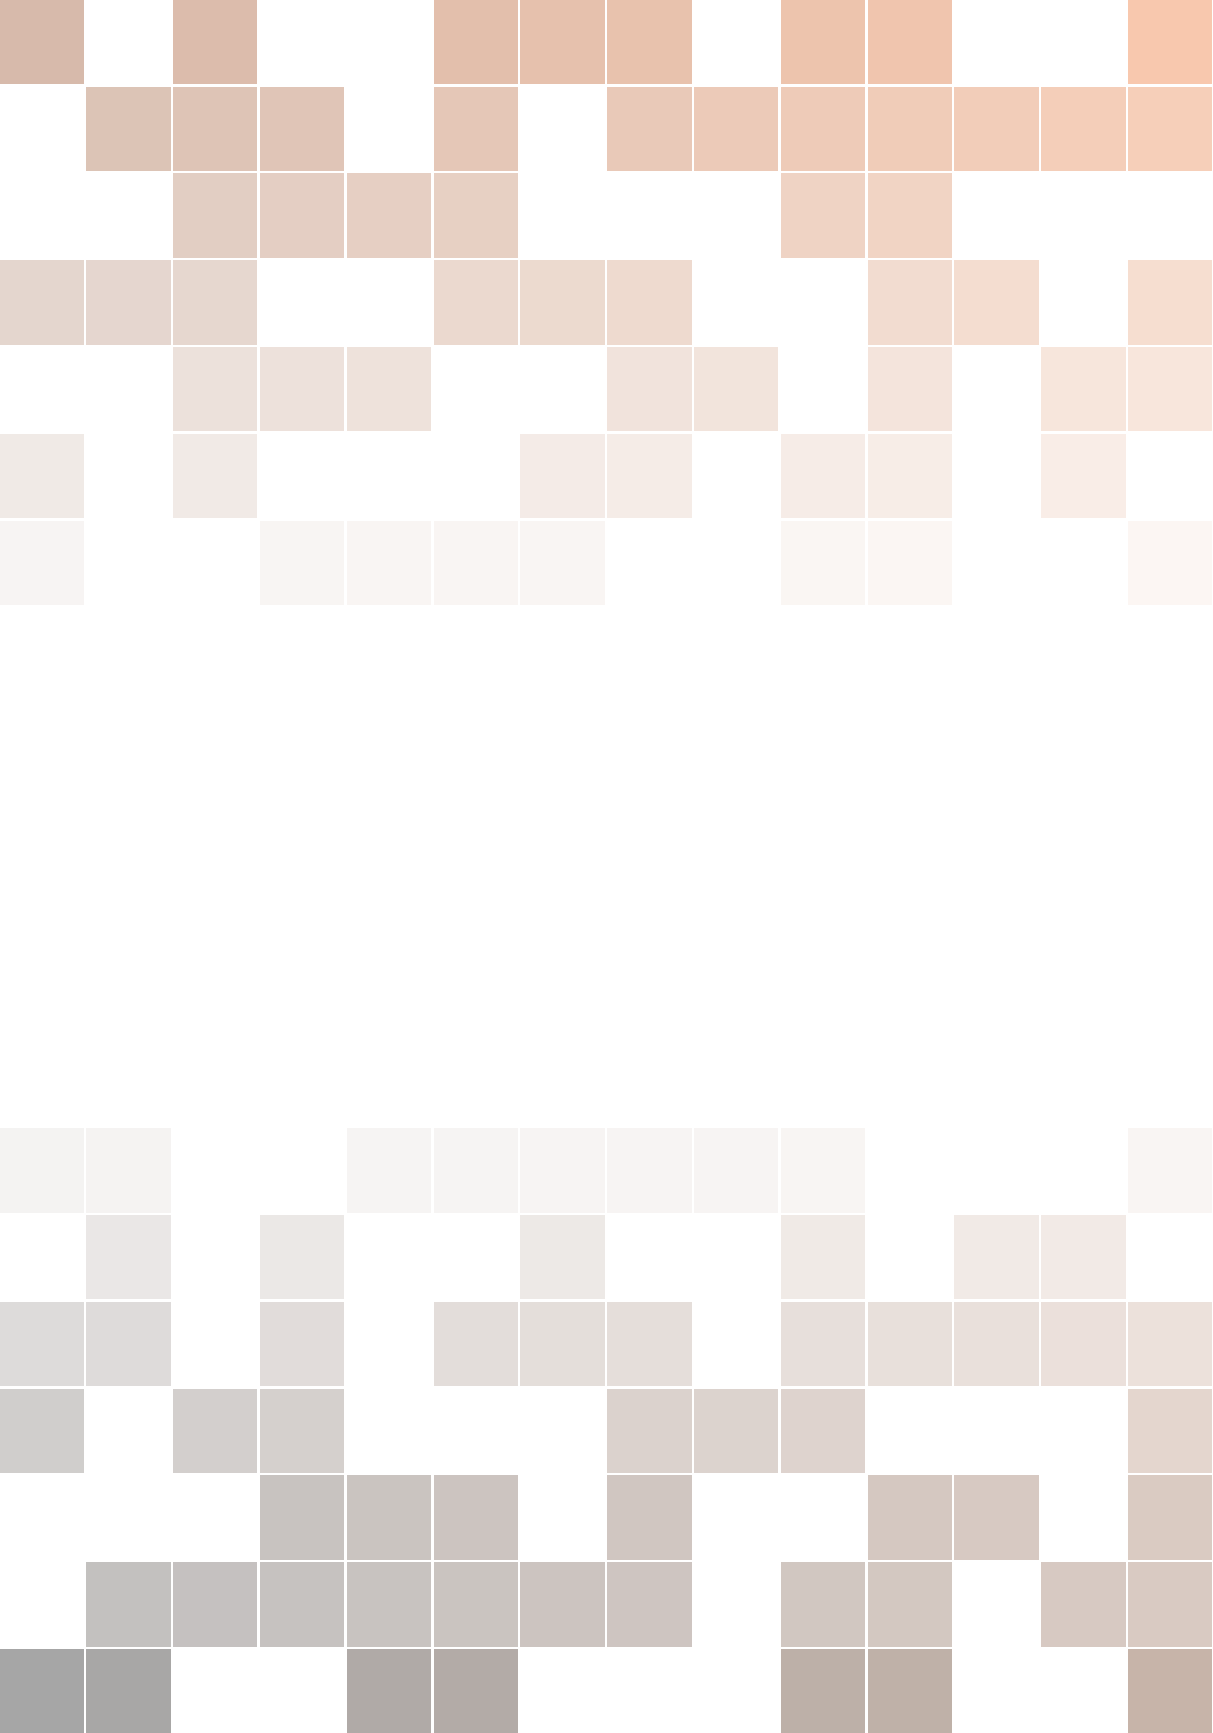
\includegraphics[scale=1]{background}}} % Image background
\centering
\vspace*{9cm}
\par\normalfont\fontsize{35}{35}\sffamily\selectfont
Kli{\ng}on Language and Culture\par % Book title
\vspace*{0.5cm}
\small{so kli{\ng}onáse khaban niso}\par
\vspace*{1cm}
{\Huge Mnajai Kot Singh}\par % Author name
\endgroup

%----------------------------------------------------------------------------------------
% COPYRIGHT PAGE
%----------------------------------------------------------------------------------------

\newpage
~\vfill
\thispagestyle{empty}

\noindent Copyleft \copyright\ 2378-2379 Mnajai Kot Singh, All Rights Reversed\ % Copyright notice

\noindent \textsc{Published by The Vulcan Academy of Sciences}\\ % Publisher

\noindent \textsc{intercore://vulcanacademy.edu}\\ % URL

\noindent Permission is granted to copy, distribute and/or modify this document under the terms of the GNU Free Documentation License, Version 1.3 or any later version published by the Free Software Foundation; with no Invariant Sections, no Front-Cover Texts, and no Back-Cover Texts.\\ % License information

\noindent \textit{First printing, March 2378} % Printing/edition date

%----------------------------------------------------------------------------------------
% TABLE OF CONTENTS
%----------------------------------------------------------------------------------------

% \chapterimage{chapter_head_1.pdf} % Table of contents heading image

\pagestyle{empty} % No headers

\tableofcontents{klingon} % Print the table of contents itself

\cleardoublepage % Forces the first chapter to start on an odd page so it's on the right

\pagestyle{fancy} % Print headers again

%----------------------------------------------------------------------------------------
% CHAPTER 1
%----------------------------------------------------------------------------------------
\chapter*{Phonology}
\addcontentsline{toc}{chapter}{Phonology}

\begin{table}[ht]
  \caption{Consonants}
  \centering
  \begin{tabular}{ l l }
  \hline\hline
    b & as in \textbf {b}oy when at the beginning, \\
    & as in \textbf{b}ueno when in the center, or end of a word  \\
    d & as in \textbf {d}ad \\
    f & as in \textbf {f}orthwith \\
    g & as in ju\textbf {g} \\
    h & as in \foreignlanguage{russian}{\textbf{х}воя} or lo\textbf {ch} \\
    j & as in \textbf{g}iraffe as the beggining orl end, lei\textbf{su}re in the middle \\
    k & as in \textbf{K}aiser \\
    kh & as in k + h said together \\
    l & as in \textbf{l}ollipop \\
    m & as in \textbf{m}om \\
    n & as in \textbf{n}ever \\
    ŋ & as in \textbf{Ng}uyen \\
    p & as in \textbf{p}apa \\
    r & as in che\textbf{r}che \\
    s & as in \textbf{sh}ake \\
    t & as in \textbf{t}ell \\
    ts & as in \textbf{ts}e-tse fly \\
    v & as in \textbf{v}ideo \\
    x & as in tri\textbf{x} \\
    y & as in \textit{y}es when at the beginning, like \textbf{ya} when at the end \\
    z & like \textbf{uhz} where the h is very soft \\
    \hline
  \end{tabular}
  \label{table:consonants}
\end{table}

\begin{table}[ht]
  \caption{Vowels and Diphtongs}
  \centering
  \begin{tabular}{ l l }
    \hline\hline
    a & as in f\textbf {a}ther  \\
    á & as in h\textbf {ay}  \\
    æ & as in \textbf{æ}vum \\
    e & as in b\textbf {e}t \\
    é & as in pa\textbf {yee} \\
    i & as in b\textbf{ee} when at the beginning or end, as in b\textbf{i}t in the middle \\
    o & as in \textbf{e}pilate when at the begining, as in b\textbf{o}t in the middle \\
    ó & as s\textbf{oa}p \\
    \hline
  \end{tabular}
  \label{table:vowels}
\end{table}
%----------------------------------------------------------------------------------------
% CHAPTER 2
%----------------------------------------------------------------------------------------
\chapter*{Grammar }
\addcontentsline{toc}{chapter}{Grammar }

\section*{Nouns}
\addcontentsline{toc}{section}{Nouns, Pronouns and Adjectives}

\klingonl groups nouns and pronouns together. There are only single pronouns, Me, You, Him, Her, It, Them, That.\par


\begin{table}[ht]
	\caption{Personal Pronouns}
	\centering
	\begin{tabular}{ l l }
		\toprule
		\english				& 	\klingonl 		\\
		\midrule
		I/Me/Myself 			&	u 				\\
		You(singular) 			&	g\'{a} 			\\
		You(plural) 			&	ng\'{a} 		\\
		He/Him 					&	jot 			\\
		She/Her 				&	sa'an 			\\
		it 						&	kan 			\\
		it(indefinite) 			&	la 				\\
		Them/They 				&	ku'ul 			\\
		This 					&	suj 			\\
		These 					&	sujm\'{a} 		\\
		That 					&	soj 			\\
		Those 					&	sojm\'{a} 		\\
		Here 					&	elov 			\\
		There 					&	ya 				\\
		\bottomrule
	\end{tabular}
	\label{table:personal_pronouns}
\end{table}

Nouns agglutinate certain particles or even other nouns and pronouns that can modify them. In the case of pronouns. Consider this table.\par

\begin{table}[ht]
	\caption{Impersonal Pronouns}
	\centering
	\begin{tabular}{ l l l l   }
		\toprule
				& Interrogative 			& Demonstratives 			& 				\\	
		\midrule
		Adj. 	& which 					& this 			 			& that 			\\	
				& suja'na/soja'na 			& suj 						& soj 			\\	
		Person 	& who 						& this(one) 				& that(one) 	\\
				& klina					 	& klin suj 					& klin soj		\\
		Thing 	& what 						& this(one) 				& that(one) 	\\
				& kana		     			& suj 						& soj 	 		\\
		Place 	& where 					& here 						& there 		\\
				& ya'na 					& elov		 				& ya 			\\
		\bottomrule
	\end{tabular}
	\label{table:impersonal_pronouns_1}
\end{table}

When referring to unknown or uncertain quantities, like some, \vocab{la} is used. \vocab{la} is the 
indefinite actor used also in the passive voice \phrase{ng\'{a} la zhal - you are remembered}.

\begin{table}[ht]
	\caption{Impersonal Pronouns Cont.}
	\centering
	\begin{tabular}{ l l l l }
		\toprule
				& Indefinite 			& 					& 							\\
		\midrule
		Adj. 	& some 					& none 				& every 					\\
				& la 		  			& la'b\'{a} 		& sor 						\\
		Person 	& someone 				& no one 			& everyone 					\\
				& laklin 				& lab\'{a}klin 		& sora'klin 				\\
		Thing 	& something 			& nothing 			& everything 				\\
				& lakan			 		& lakanb\'{a} 		& sorkan 					\\
		Place 	& somewhere 			& nowhere 			& everywhere 				\\
				& laya 					& layab\'{a} 		& sorya 					\\
		\bottomrule
	\end{tabular}
	\label{table:impersonal_pronouns_2}
\end{table}

As we see in Table \ref{table:impersonal_pronouns_1} and Table \ref{table:impersonal_pronouns_2} the pronouns glue together to into a compound pronoun like \defn{sor}{all} with \defn{ya}{there} to form \defn{sorya}{everywhere}. In the case of \defn{klina}{who} we have an example of the disappearing \'n\' in \klingonl as this is a compound pronoun with \defn{klin}{a particle having to do with people} and \defn{na}{interrogative particle}. Notice the exception in Table \ref{table:impersonal_pronouns_1} where the compound pronoun does not agglutinate but is isolating and inverted. You would expect \vocab{sujklin} or even \vocab{klinsuj} here. This is one of the many exceptions to be found in \klingonl, due to the hodgepodge nature of \klingonl source languages. \place{Sig\'{o}r} province is known as the Savoyan Source \vocab{thadon \name{savoy}}, and it's features are agglutination and OSV word order. \place{Mithrot} province provides the Mithrotian Source \vocab{thadon \place{mithrot}} which has distinctly Latin features in that verbs are inflected, but only for person and number. 

\klingonl was all but destroyed during the \name{hurk} invasion in 940 C.E.\footnote{\english dating is used in this text for the readers convience.}. Once the invaders had been repelled\footnote{The \name{hurk} empire crumbled from within, it would be several millenia before \klingons would admit that they had little to do with getting rid of them.}, \klingons wanted to recover their lost heritage, but the \name{hurk} suppression of traditional culture and language had been so complete, and the \klingons were in such a state of economic and cultural ruin, that they hardly knew where to start. Almost all literary works had been burnt, inscriptions scraped out, temples demolished. What did survive was extremely old and practically useless. \klingons were mixed ethnically, in an attempt to insure that no nonds of culture could be maintained, and what passed for \klingonl at that time was little more than a pidgin dialect.

The wise elders of the day did the only thing they could. They made it all up. They had a wide variation of pidgin dialects, very few examples of old \klingon and one or two inscriptions and so they went about recreating the entire language from scratch.  When this was complete a dictionary was made and any missing words were added on the fly. Because a huge quantity of words in the lexicon were \name{hurk}, they had to be removed and new \klingon words were generated. Some more consistently and well thought out than others.

The \name{hurk} occupation of \name{kronos} had scarred and mangled the \klingon spirit, but they were resolved to be reborn from the ashes with a philosophy of never again being crushed under the boot of an invader\footnote{Unfortunately this didn't extend to crushing each other under \klingon boots. Shortly after throwing off the \name{hurk}, \klingons entered the Five Tyrants Period.}. In this new spirit of comraderie and equality it was decided that everyones linguistic peculiarities were at least partially right, and so a great many exceptions and deviations made it into the language to accommodate the modes of speech of various regions.

\begin{table}[ht]
	\caption{Noun Particles and Suffixes}
	\centering
	\begin{tabular}{ l l l }
		\toprule
		a- & N-yu & predictive progressive, afloat, awash \\
		ambi- & N-nu & both \\
		amphi- & otor N & around, surround \\
		ana- & N-ede & up, back, anew \\
		ano- & N-ede & up, back, anew \\
		ante- & krim N & before \\
		ant- & krim N & before \\
		anti- & N-sus & against,opposite \\
		apo- & suru N & away from \\
		arch- & N-'os & supreme, highest, best, biggest \\
		be- & N-vav & equipped with, covered with \\
		bi- & N-nu & both of two \\
		bibl- & vral N & book, having to do with books \\
		bibli- & vral N & book, having to do with books \\
		biblio- & vral N & book, having to do with books \\
		bio- & N-oke & having to do with biological things \\
		cad- & N-jon & to seize \\
		cap- & N-jon & to seize \\
		caus- & N-mek & burn, heat \\
		circum- & otor N & around, about, surrounding \\
		co- & utsul N & joint, accompanying, with \\
		cog- & utsul N & joint, accompanying, with \\
		col- & utsul N & joint, accompanying, with \\
		com- & utsul N & joint, accompanying, with \\
		con- & utsul N & joint, accompanying, with \\
		contra- & N-sus & against,opposite \\
		counter- & N-sus & against,opposite \\
		corp- & torgh N & body \\
		de- & N-lus & not, reverse action, opposite \\
		dec- & N-mah & ten, 10 \\
		deca- & N-mah & ten, 10 \\
		dis- & N-lus & not, opposite of \\
		dif- & N-lus & not, opposite of \\
		dict- & jatl N & speaking, saying \\
		dei- & N-kun & god \\
		divi- & N-kun & god \\
		div- & N-lis & separate \\
		demo- & klin N & people \\
		doc- & N-goj & teach \\
		dual- & N-nu & both of two \\
		dys- & luja N & fail, fault \\
		ec- & N-dek & out of, from \\
		eco- & hyul N & household, environment, local area \\
		ecto- & N-dek & out of, from \\
		en- & N-bal & get into, enmesh \\
		endo- & N-æs & within, inside \\
		em- & N-bal & get into, put into, empower \\
		ex- & N-mu & former \\
		\bottomrule
	\end{tabular}
	\label{table:prefixes_1}
\end{table}

As we see with Table \ref{table:prefixes_1} \& \ref{table:prefixes_2} there is a correlation between \english prefixes and \klingon particles. This is a general table of rough equivalents, there really isn't a 1-to-1 correlation, and many compound \english words that take a prefix or suffix have a their own word in \klingon that doesn't include particles from these tables.

\begin{table}[ht]
	\caption{Noun Particles and Suffixes Cont.}
	\centering
	\begin{tabular}{ l l l }
		\toprule
		lang- & áse N & having to do with language, a tool \\
		fore- & krim N & before, in front \\
		hind- & adah N & after \\
		mal- & usul N & bad, badly \\
		mid- & hraj N & middle, between \\
		mini- & N-om & small, miniature \\
		mis- & N-'œ & wrong, astray \\
		out- & N-'os & better, faster \\
		over- & hotsil N & excessive, above \\
		peri- & ulari N & around, near, nearby \\
		post- & N-ada & after,behind \\
		pro- & N-guj & for, on the side of \\
		pre- & krim N & before, in front \\
		pseudo- & N-som & fake, false, misrepresent \\
		re- & N-gul & again \\
		self- & N-ag & self, self-sufficient \\
		sep- & N-lis & divied, pull apart \\
		soci- & N-dat & having to do with society \\
		sub- & N-om & below \\
		sup- & N-om & below, under \\
		super- & N-'os & above, higher \\
		supra- & N-'os & above, higher \\
		sur- & N-'os & above, higher \\
		ultra- & N-'os & above, higher \\
		tele- & N-kuk & distance, range, from a distance \\
		trans- & rats N & through, across \\
		un- & N-sus & not, against \\
		uni- & N-mev & one, together, united \\
		under- & N-om & lower, lesser, under, beneath \\
		up- & N-'os & greater, higher \\
		with- & N-sus & against, withstand \\
		\bottomrule
	\end{tabular}
	\label{table:prefixes_2}
\end{table}
As we see in Table \ref{table:suffixes_1} there are also rough equivalents to \english suffixes. 
\begin{table}[ht]
	\caption{Noun Particles and Suffixes Cont.}
	\centering
	\begin{tabular}{ l l l }
		\toprule
		-an & N-yi' & one who does \\
		-ance & N-jub & action of state of \\
		-ancy & jub' N & state, quality, or capacity \\
		-ant & N-si' & something that does, performs \\
		-ard & dokjo N & characterized as, like \\
		-ary & dokjo N & resemble, like \\
		-cide & hotoh N & kill \\
		-ent & N-si' & something that does, performs \\
		-fold & dokjir N & in a manner marked by, fourfold \\
		-ful & N-boh & filled, full with \\
		-fy & bakha N & make, form \\
		-ish & dokjo N & resemble, like \\
		-ism & N-kul & doctrine, conduct, belief \\
		-ist & N-yi' & one who does \\
		-ology & N-ked & the science of \\
		-nomy & okedi N & the science of naming, having to do with names \\
		-onymy & ási N & specified, named, or naming \\
		-onym & ási N & specified, named, or naming \\
		-language & áse N & tool, language \\

		\bottomrule
	\end{tabular}
	\label{table:suffixes_1}
\end{table}



\clearpage

\section*{Verbs }
\addcontentsline{toc}{section}{Verbs and Adverbs }

\klingonl verbs inflect to indicate person, and adverbs which modify them directly follow the verb and agree in person. \defn{sal}{to run} becomes \defn{sesa}{I run, am running}. To say I am running fast you would use the adverb \defn{tsefut}{fast, quickly} as \phrase{sesa tsefesa}. Tense is not inflected in the verb, but it presents as a particle that \textit{usually} appears at the beginning of a phrase as in \phrase{yaisg sesa - I ran} and could be used in a sentence such as \phrase{yaisg porahndak sesa - I ran to the store}. \klingonl tenses are very precise in the short term for future and past, \phrase{soto porahndak sesa - earlier today I ran to the store}. There is nothing that actually requires this word order, but it is the most common. You could say \phrase{otor porahn sesa tsefesa soto - earlier today I ran around the store}. The same would work for \phrase{sesa tsefesa soto otor porahn}. It is considered a sign of poor education to do this. The general structure of \klingonl phrases are Tense, Object, Subject, Verb. Any other order would be a little weird and out of the ordinary, but \klingons have learned to deal with foreigners, and they have a very liberal linguistic heritage. There is no \klingon concept of a \textbf{grammar nazi}.

That being said, there is a right way and a wrong way, limited poetic constructions notwithstanding, you should adhere to the rules as closely as possible. Deviate from them only occasionally, perhaps to emphasize a point.

In \english there is the concept of a phrasal adverb, such as \phrase{I ran to the store quickly.} \klingonl does not do this, it is a strict rule in \klingonl that an adverb follows a verb. The above can be accomplished with a \textit{tense adjective}. Adjectives usually follow nouns, but when they follow a tense word they modify the entire phrase. Consider: \phrase{yaisg tsebas porahndak sesa - I ran to the store quickly}.

\section*{Particles}
\addcontentsline{toc}{section}{Particles}

Up to this point you have seen many particles and suffixes (they are considered in the same class) in action. \klingonl particles are very versatile, they can take as their "argument" any other \klingonl word (including other particles!) and they will consistently modify it. Some combinations while grammatically correct are of course non-sensical. There are som restrictions to this, for instance free floating particles, e.g. those that do not agglut cannot modify an agglutinating particle. Setting two free floating particles next to each other will make the first modify the second, and the combined meaning of those will then modify whatever follows. In some cases, this is not desired, so it is possible to separate the particles with a \defn{pa}{nul particle}.

%----------------------------------------------------------------------------------------
% Afterword
%----------------------------------------------------------------------------------------
\chapter*{OOC Afterword }
\addcontentsline{toc}{chapter}{OOC Afterward }

\begin{quote}
People like to be told what they already know.  Remember that.  They get uncomfortable when you tell them new things.  New things…well, new things aren’t what they expect.  They like to know that, say, a dog will bite a man.  That is what dogs do.  They don’t want to know that a man bites a dog, because the world is not supposed to happen like that.  In short, what people think they want is \textit{news}, but what they really crave is \textit{olds}. - \textbf{Terry Pratchett}
\end{quote}

In designing an alien world, it is important to remember not to make it too alien. This is the mantra of most concept designers. When they imagine alien machines, or buildings, or insects they know that they are constrained by two things, physics and biology, and how their audience \textit{thinks} they understand physics and biology\footnote{Blast Ended Skrewts notwithstanding}. You are always limited by what your audience can believe is possible. It's much broader than you think, but it is not infinite. The suspension of disbelief can never be pushed so far that it becomes the suspension of reason.

The limits on what is conceivable for a culture would seem to not have this issue. Why should an alien culture adhere to any human sociological, psychological, or even ethical standards? You would think that you have a much wider field in which to maneuver, but you would in fact be completely wrong. The purpose of a successful alien culture, that is one where people would want to dress up like them, learn their con-lang, and fantasize about adventures on their homeworld, is not to be alien, but to be a mirror. We want attributes, mores, and norms that we find inside ourselves magnified and reflected back to us. No one wants to visit the Borg homeworld. Unless they have a cyborg-amputee fetish. The Borg are too alien.\footnote{Until the introduction of the Borg Queen, the Borg were very nebulous baddies.} I imagine few people fantasize about romantic encounters in the assimilation chamber. Voyager and later TNG movies went a long way to humanizing the Borg. Alice Krige in the role of The Borg Queen is a case in point. The hive-mind of the Borg became a little more litteral, and suddenly people were much more interested in the social structure of the Borg. They still haven't been completely rehabilitated, but I imagine future Star Trek will retcon them into pointlessness.

\clearpage

\begin{quote}
I must tell you I'm disappointed at hearing you mouth the usual platitudes of peace and friendship regarding an implacable foe like the Romulans. But I live in hope that you may one day see the universe for what it truly is, rather than what you'd wish it to be. - \textbf{Elim Garak}
\end{quote}

\begin{quote}
Well, I shall endeavor to become more cynical with each passing day, look gift hordes squarely in the mouth, and find clouds in every silver lining. - \textbf{Julian Bashir}
\end{quote}

\begin{quote}
If only you meant it. - \textbf{Elim Garak}
\end{quote}

Even in the case of the Vulcans, the Federations closest Allies, they are constantly presented as less than humans, with much to learn about the right way of existing. Vulcans have been heavily retconned into incredulity. Despite their outward appearance of dispassion and logic, they are consistently portrayed as highly emotional, or in desperate need of some kind of emotional intelligence that can usually only be provided by a human counterpart. It's rather sad that their entire culture is based on such a false premise as the supremacy of logic and dispassionate scientific enquery. Enterprise made immense strides in sexualising the Vulcans as well, and the character T'Pol is often bordering on ridiculous with her constant posturing in cat suits. 

Enterprise didn't stop there in its effort to degrade the Vulcan Culture where they are presented as stale, self-serving, and propagandist. Apparently there are even emotionally \textit{free} Vulcans. T'Pol needs to be instructed on how to perform mind melds by a human. Apparently the thin veneer of logic can even be broken by jazz music! It's all a bit ridiculous. Considering the lack luster support for Star Trek, I can only conclude that this trend is having a predominantly negative effect on the franchise. The latest Star Trek movies, while box office smashes, are beneath consideration in every possible way.

It is essential that an alien race only diverge at a few key points, and their divergence must be counter-balanced by the enlargement of at least one positive feature. The \klingons may be violent, loud, and filthy but their oversized sense of honor and loyalty make them more palatable. While Kirk makes the comparison between the \klingons and Nazi Germans in \movie{Undiscovered Country}, they really aren't that way at all, and never could be. If there is not a key feature enlarged to compensate, then we must at least observe a motivation to change the negative aspects of the culture. The Ferengi would be intolerable if it weren't for Moogie and the progressive Zek. The fact that women are, by human standards, horribly objectified, sexualized, and enslaved would be completely intolerable if there wasn't some feminist effort to change. It does leave one to wonder, would an alien races female members ever be happy in servitude? Of course not, because that is one of the many taboos or morals of our culture. It is very important that no serious taboo or too widely accepted moral be broken or assailed unless there is a strong counter-balancing element. 

A taboo is a prohibition based on the belief that the behavior is either too sacred or too accursed for people to engage in it. While human culture doesn't have any universal taboos, there are a number of them that are particularly strong in the west. The english speaking west being the most likely consumer of Star Trek related material.

\begin{enumerate}
	\item Incest
	\item Necrophilia
	\item Adultery
	\item Fornication
	\item Pedophilia
	\item Beastiality
	\item Cannibalism
	\item Infanticide
	\item Murder
\end{enumerate}

It is not that people don't commit taboos, it is that they will 1) feel uncomfortable discussing them 2) conceal them or any knowledge of them, and 3) require an \textit{abjure} statement about them. You know you are talking about a taboo when you feel the need to prefix what you say with, of course \textit{x} is horribly wrong, inexcusable, repugnant, disgusting, and any number of negative adjectives. The more vitriol the better.

Different classes of people may also have taboos against inter-racial marriage, homosexuality and even religious inter-marriage. Humans have a suspiciously large number of sexual and mating taboos.

Another important feature of a society is its morals, in the sense of things you have learned, or think you have learned. These are tacit truths about human behavior. You know you are dealing with a moral when you find yourself prefixing statements with \textit{Obviously ...} and \textit{Everyone knows/accepts/understands that}.

\begin{enumerate}
	\item It is better to be poor than rich, or at least the rich must be very unhappy
	\item Violence is never the answer. Those who live by the sword, die by the sword
	\item Everyone makes mistakes, even the government, that's why democracy is the best system \ldots
\end{enumerate}

The Ferengi obviously violate number one, being obscessed with money, they are unhappy, and Quark always finds himself most satisfied when he violates Ferengi cultural mores and increases wages, or grants workers rights, or makes some sort of donation to the Bajoran Orphan's Fund. The \klingons violate number two, and usually end up being reasoned to a more peaceful solution. One begins to wonder how they've survived this long without the Federation there to explain that one too them. The Cardassians violate number three, and a great deal of plot fodder centers around their totalitarian political system. They are just about to go democratic when the Dominion sweeps in. We are left with the impression from Garak at the end of DS9 that things will be changing for the better. Other ones violated are those like 1) women are intrinsically equal to men(the Ferengi), 2) People are innocent until proven guilty(Cardassians), and 3) pride goeth before a fall(Romulans).

Morals are sometimes a bit timeless, that is they have been around for a long time, and others are era dependent. Everyone knows that smoking is bad, obviously eating too much fat can cause a heart attack and so on. Morals are not right or wrong by virtue of being a moral. Sometimes everyone knows what is right to be right and sometimes everyone knows what is wrong to be right. Critical thinking is a must.

\begin{quote}
No one can be a great thinker who does not recognise, that as a thinker it is his first duty to follow his intellect to whatever conclusions it may lead. Truth gains more even by the errors of one who, with due study and preparation, thinks for himself, than by the true opinions of those who only hold them because they do not suffer themselves to think. - \textbf{John Stuart Mill}
\end{quote}

With the exception of Farscape and the Sebaceans, Humans are generally the good guys, and everyone else must invariably be less than us. No one wants to fantasize about their race being seen as a pariah on the galaxy after all. Humans must invariably triumph, and most importantly they must triumph because of what we imagine are our good qualities. We must win because we are optimistic, persevering, benevolent and peace loving\footnote{Opinions that human history sutbbornly refuses to bare out.}. It is very important that we protect ourselves from our inherent weaknesses and moral and ethical frailties. Even though DS9 made great strides to undo fascist starfleet propaganda by mixing in some conspiracies, and even an ultra-secret spy death squad Section 31\footnote{Even in this case, all the build up was undone in \textbf{Inter Arma Enim Silent Legis}}, these are always to be presented as the exception rather than the rule. Any evil we do must be portrayed as an honest mistake, a well intentioned genocide here, and unfortunate world war there. But let's not descend too far into human hating. It is not that humans are all bad or all good, but more complex than we are willing to admit. So must be other races.

What is great about humanity is that there is something for everyone, even evil people. Of course, Hitler didn't wake up in the morning, look in the mirror and say \"Today I am going to be evil!\". He probably thought he was a great guy. Most of history doesn't agree, but that's more common than you think. Obviously there are people in this world who like taking candy from babies, metaphorically and perhaps literally as well. The possibilities of naughtiness abound. From kink to killing, somewhere and somewhen there is a place for every type of human being. We may not like it, but there it is. It is what makes humanity something worth existing. A utopia would suck for most people, as Pat Califia noted\footnote{I am here referring to her essay Whoring in Utopia.}.

As it stands, the world of today would invariably be the \#1 tourist destination for the entire galaxy, because for a price almost anything can be had. In the end, what makes a society interesting and immersive is that it is some place you'd want to visit. Most alien societies fail this test in spades. No person in their right mind would ever want to visit Kronos as it is described, or Romulus, or Ferenginar. Vulcan wouldn't be much of a tourist stop either come to think about it. Unless you are really into dry formalized debates and lots of meditating, but then that's only a small portion of the entire human population. The question you should ask about your alien society is: How likely is MTV to want to film a spring break special there\footnote{I am only slightly kidding.}?

This all depends on what kind of society you want to create. You may just need a bunch of paper tiger baddies. Maybe your intention is to create a society for inverse comparison against humans? Maybe you don't really care all that much. It's like a house. In a pinch just about any structure will do against the rain, but would you actually want to live there? 







%----------------------------------------------------------------------------------------
% Dictionaries
%----------------------------------------------------------------------------------------
\twocolumn
\chapter*{English to Kli{\ng}onáse Dictionary}
\addcontentsline{toc}{chapter}{English to Kli{\ng}onáse Dictionary}

\clearpage
% \subsection*{A}

\entry{a} \pos{noun} (biochemistry) purine base found in DNA and RNA; pairs with thymine in DNA and with uracil in RNA: \vocab{heorej}. one of the four nucleotides used in building DNA; all four nucleotides have a common phosphate group and a sugar (ribose): \vocab{hiedej}. any of several fat-soluble vitamins essential for normal vision; prevents night blindness or inflammation or dryness of the eyes: \vocab{hatej}.

\entry{a-one} \pos{adjective} of the highest quality: \vocab{krilas}.

\entry{able} \pos{adjective} (usually followed by `to') having the necessary means or skill or know-how or authority to do something \textit{or} having inherent physical or mental ability or capacity \textit{or} have the skills and qualifications to do things well: \vocab{veohet}. having a strong healthy body: \vocab{tsuras}.

\entry{able-bodied} \pos{adjective} having a strong healthy body: \vocab{tsuras}.

\entry{abound} \pos{verb} be in a state of movement or action: \vocab{lemal}.

\entry{about} \pos{adjective} on the move: \vocab{sætu}.

\entry{about} \pos{adverb} (of quantities) imprecise but fairly close to correct: \vocab{tæjut}. in the area or vicinity: \vocab{tayut}. all around or on all sides: \vocab{tæfut}. in or to a reversed position or direction: \vocab{toyut}. used of movement to or among many different places or in no particular direction: \vocab{tærut}. (of actions or states) slightly short of or not quite accomplished; all but: \vocab{tusut}. in rotation or succession: \vocab{tobut}.

\entry{abut} \pos{verb} lie adjacent to another or share a boundary: \vocab{jaratl}.

\entry{accept} \pos{verb} receive willingly something given or offered: \vocab{todal}. make use of or accept for some purpose: \vocab{kesal}. admit into a group or community: \vocab{keamal}. be designed to hold or take: \vocab{kidal}.

\entry{accession} \pos{noun} something added to what you already have: \vocab{maigahn}.

\entry{accommodation} \pos{noun} making or becoming suitable; adjusting to circumstances: \vocab{flæhon}.

\entry{accompany} \pos{verb} be a companion to somebody: \vocab{kivul}.

\entry{accord} \pos{noun} harmony of people's opinions or actions or characters: \vocab{reavoj}.

\entry{account} \pos{noun} the quality of taking advantage: \vocab{kædan}. importance or value: \vocab{keotan}. a record or narrative description of past events: \vocab{kuntan}. an itemized statement of money owed for goods shipped or services rendered \textit{or} a short account of the news: \vocab{keohan}. a statement that makes something comprehensible by describing the relevant structure or operation or circumstances etc. \textit{or} a formal contractual relationship established to provide for regular banking or brokerage or business services: \vocab{keagan}. the act of informing by verbal report: \vocab{kietan}. grounds: \vocab{kuntran}. a statement of recent transactions and the resulting balance: \vocab{kestan}.

\entry{account} \pos{verb} furnish a justifying analysis or explanation: \vocab{leolul}. to give an account or representation of in words: \vocab{lælul}. keep an account of: \vocab{laihul}. be the sole or primary factor in the existence, acquisition, supply, or disposal of something: \vocab{laimul}.

\entry{accounting} \pos{noun} a statement of recent transactions and the resulting balance: \vocab{kestan}.

\entry{accredit} \pos{verb} ascribe an achievement to: \vocab{mithatl}.

\entry{accrue} \pos{verb} come into the possession of: \vocab{gupik}.

\entry{ace} \pos{adjective} of the highest quality: \vocab{krilas}.

\entry{acknowledge} \pos{verb} accept (someone) to be what is claimed or accept his power and authority: \vocab{saxul}.

\entry{acknowledgment} \pos{noun} a short note recognizing a source of information or of a quoted passage: \vocab{khearahd}.

\entry{acquaintance} \pos{noun} a person with whom you are acquainted: \vocab{zhán}.

\entry{acquire} \pos{verb} come to have or undergo a change of (physical features and attributes): \vocab{vijal}. come into the possession of something concrete or abstract: \vocab{lagul}. take on a certain form, attribute, or aspect: \vocab{kienal}.

\entry{acquisition} \pos{noun} the cognitive process of acquiring skill or knowledge: \vocab{praloj}.

\entry{acres} \pos{noun} extensive landed property (especially in the country) retained by the owner for his own use: \vocab{jæton}.

\entry{across} \pos{adverb} transversely \textit{or} to the opposite side: \vocab{kifase}.

\entry{act} \pos{verb} behave in a certain manner; show a certain behavior; conduct or comport oneself: \vocab{thaizul}. have an effect or outcome; often the one desired or expected: \vocab{theolal}. pretend to have certain qualities or state of mind: \vocab{giegal}. discharge one's duties: \vocab{gæjal}. play a role or part: \vocab{gastal}. perform on a stage or theater: \vocab{gearal}. behave unnaturally or affectedly: \vocab{gantral}. perform an action, or work out or perform (an action): \vocab{gagyal}. be engaged in an activity, often for no particular purpose other than pleasure: \vocab{gestal}. be suitable for theatrical performance: \vocab{gaipal}.

\entry{act} \pos{noun} a short theatrical performance that is part of a longer program: \vocab{vopahd}. something that people do or cause to happen: \vocab{bæloj}. a legal document codifying the result of deliberations of a committee or society or legislative body: \vocab{biedoj}. a subdivision of a play or opera or ballet: \vocab{bæmoj}. a manifestation of insincerity: \vocab{beodoj}.

\entry{ad} \pos{noun} a public promotion of some product or service: \vocab{thathej}.

\entry{adam} \pos{noun} street names for methylenedioxymethamphetamine: \vocab{k'aizon}.

\entry{adaptation} \pos{noun} the process of adapting to something (such as environmental conditions): \vocab{fleopon}.

\entry{adaption} \pos{noun} the process of adapting to something (such as environmental conditions): \vocab{fleopon}.

\entry{add-on} \pos{noun} a component that is added to something to improve it: \vocab{mægahn}.

\entry{addition} \pos{noun} the act of adding one thing to another: \vocab{mearahn}. the arithmetic operation of summing; calculating the sum of two or more numbers: \vocab{murkahn}. a component that is added to something to improve it: \vocab{mægahn}. a suburban area laid out in streets and lots for a future residential area: \vocab{mielahn}. something added to what you already have: \vocab{maigahn}. a quantity that is added: \vocab{meohahn}.

\entry{address} \pos{verb} greet, as with a prescribed form, title, or name: \vocab{yijal}. act on verbally or in some form of artistic expression: \vocab{vuthul}.

\entry{adenine} \pos{noun} (biochemistry) purine base found in DNA and RNA; pairs with thymine in DNA and with uracil in RNA: \vocab{heorej}.

\entry{adept} \pos{adjective} having or showing knowledge and skill and aptitude: \vocab{yeogas}.

\entry{adjacent} \pos{adjective} nearest in space or position; immediately adjoining without intervening space: \vocab{rahet}.

\entry{adjoin} \pos{verb} lie adjacent to another or share a boundary: \vocab{jaratl}.

\entry{adjudicate} \pos{verb} put on trial or hear a case and sit as the judge at the trial of: \vocab{misik}.

\entry{adjustment} \pos{noun} the act of making something different (as e.g. the size of a garment):  \vocab{flævon, flævon} . the act of adjusting something to match a standard \textit{or} an amount added or deducted on the basis of qualifying circumstances:  \vocab{flugyon, flugyon} . making or becoming suitable; adjusting to circumstances:  \vocab{flæhon, flæhon} . the process of adapting to something (such as environmental conditions):  \vocab{fleopon, fleopon} .

\entry{administration} \pos{noun} the act of governing; exercising authority: \vocab{yizarn}. the persons (or committees or departments etc.) who make up a body for the purpose of administering something: \vocab{heatan}.

\entry{admirer} \pos{noun} a person who backs a politician or a team etc.: \vocab{kurofej}.

\entry{admit} \pos{verb} admit into a group or community: \vocab{keamal}.

\entry{adopt} \pos{verb} take on a certain form, attribute, or aspect: \vocab{kienal}.

\entry{adult} \pos{adjective} (of animals) fully developed: \vocab{beset}.

\entry{advancing} \pos{adjective} moving forward: \vocab{thielu}.

\entry{advantageously} \pos{adverb} in a manner affording benefit or advantage: \vocab{ventrut}.

\entry{adventure} \pos{verb} take a risk in the hope of a favorable outcome: \vocab{ohleojatl}.

\entry{advert} \pos{noun} a public promotion of some product or service: \vocab{thathej}.

\entry{advertisement} \pos{noun} a public promotion of some product or service: \vocab{thathej}.

\entry{advertising} \pos{noun} a public promotion of some product or service: \vocab{thathej}.

\entry{advertizement} \pos{noun} a public promotion of some product or service: \vocab{thathej}.

\entry{advertizing} \pos{noun} a public promotion of some product or service: \vocab{thathej}.

\entry{aerate} \pos{verb} expose to fresh air: \vocab{tsælul}.

\entry{affair} \pos{noun} a vaguely specified concern: \vocab{staijan}.

\entry{afford} \pos{verb} be the cause or source of: \vocab{hæjik}. afford access to: \vocab{biemul}.

\entry{after} \pos{adjective} located farther aft: \vocab{k'iejas}.

\entry{after} \pos{adverb} behind or in the rear: \vocab{fi'ave}. happening at a time subsequent to a reference time: \vocab{k'ulut}.

\entry{afterward} \pos{adverb} happening at a time subsequent to a reference time: \vocab{k'ulut}.

\entry{afterwards} \pos{adverb} happening at a time subsequent to a reference time: \vocab{k'ulut}.

\entry{again} \pos{adverb} anew: \vocab{zehes}.

\entry{agency} \pos{noun} how a result is obtained or an end is achieved: \vocab{k'uhej}. an administrative unit of government: \vocab{hiejoj}.

\entry{aggress} \pos{verb} take the initiative and go on the offensive: \vocab{vantal}.

\entry{aggroup} \pos{verb} form a group or group together: \vocab{hemal}.

\entry{agreement} \pos{noun} compatibility of observations: \vocab{rædoj}. the thing arranged or agreed to: \vocab{rurkoj}. the statement (oral or written) of an exchange of promises: \vocab{rentoj}. the verbal act of agreeing: \vocab{rathoj}. the determination of grammatical inflection on the basis of word relations: \vocab{reagoj}. harmony of people's opinions or actions or characters: \vocab{reavoj}.

\entry{ahead} \pos{adverb} in a forward direction: \vocab{theles}. toward the future; forward in time: \vocab{dodes}.

\entry{aid} \pos{noun} the work of providing treatment for or attending to someone or something: \vocab{fiejoj}. the activity of contributing to the fulfillment of a need or furtherance of an effort or purpose: \vocab{gentahd}. a resource: \vocab{guthan}.

\entry{aid} \pos{verb} improve the condition of: \vocab{godul}. give help or assistance; be of service: \vocab{gestul}.

\entry{aim} \pos{verb} intend (something) to move towards a certain goal: \vocab{lusal}. move into a desired direction of discourse: \vocab{fonik}. point or cause to go (blows, weapons, or objects such as photographic equipment) towards: \vocab{keojal}.

\entry{aim} \pos{noun} an anticipated outcome that is intended or that guides your planned actions: \vocab{t'eagan}.

\entry{ain} \pos{adjective} belonging to or on behalf of a specified person (especially yourself); preceded by a possessive: \vocab{li'as}.

\entry{air} \pos{verb} broadcast over the airwaves, as in radio or television: \vocab{die'atl}. expose to cool or cold air so as to cool or freshen: \vocab{tseomul}. expose to warm or heated air, so as to dry: \vocab{tseavul}. make public: \vocab{tsustul}. be broadcast: \vocab{tseapul}. expose to fresh air: \vocab{tsælul}.

\entry{air} \pos{noun} travel via aircraft: \vocab{taijon}. a distinctive but intangible quality surrounding a person or thing \textit{or} a slight wind (usually refreshing): \vocab{taston}. medium for radio and television broadcasting: \vocab{teoton}. a succession of notes forming a distinctive sequence: \vocab{tæpon}. the mass of air surrounding the Earth: \vocab{taiton}. the region above the ground: \vocab{tuntron}. a mixture of gases (especially oxygen) required for breathing; the stuff that the wind consists of: \vocab{tukkon}. once thought to be one of four elements composing the universe (Empedocles): \vocab{taŋon}.

\entry{airfield} \pos{noun} a place where planes take off and land: \vocab{eiban}.

\entry{airwave} \pos{noun} medium for radio and television broadcasting: \vocab{teoton}.

\entry{aliveness} \pos{noun} the condition of living or the state of being alive: \vocab{heson}.

\entry{alkali} \pos{noun} any of various water-soluble compounds capable of turning litmus blue and reacting with an acid to form a salt and water: \vocab{gáharn}.

\entry{all} \pos{adjective} completely given to or absorbed by: \vocab{khubet}. quantifier; used with either mass or count nouns to indicate the whole number or amount of or every one of a class: \vocab{khojet}.

\entry{all} \pos{adverb} to a complete degree or to the full or entire extent (`whole' is often used informally for `wholly'): \vocab{strivut}.

\entry{allay} \pos{verb} lessen the intensity of or calm: \vocab{deŋul}.

\entry{allege} \pos{verb} report or maintain: \vocab{jofal}.

\entry{allow} \pos{verb} make a possibility or provide opportunity for; permit to be attainable or cause to remain: \vocab{gænul}. consent to, give permission: \vocab{kopal}. make it possible through a specific action or lack of action for something to happen: \vocab{kotal}.

\entry{allowance} \pos{noun} an amount added or deducted on the basis of qualifying circumstances: \vocab{flugyon}.

\entry{ally} \pos{noun} an associate who provides cooperation or assistance: \vocab{zhán}.

\entry{almost} \pos{adverb} (of actions or states) slightly short of or not quite accomplished; all but: \vocab{tusut}.

\entry{alone} \pos{adjective} exclusive of anyone or anything else: \vocab{fæju}.

\entry{alone} \pos{adverb} without any others being included or involved: \vocab{pseohut}.

\entry{along} \pos{adverb} with a forward motion: \vocab{veahut}.

\entry{aloofness} \pos{noun} indifference by personal withdrawal: \vocab{bietan}.

\entry{alter} \pos{verb} become different in some particular way, without permanently losing one's or its former characteristics or essence: \vocab{ohluvul}. cause to change; make different; cause a transformation: \vocab{ohlaivatl}.

\entry{alteration} \pos{noun} the act of making something different (as e.g. the size of a garment): \vocab{flævon}. an event that occurs when something passes from one state or phase to another: \vocab{ohlidej}.

\entry{alternate} \pos{verb} go back and forth; swing back and forth between two states or conditions: \vocab{karsal}.

\entry{altogether} \pos{adverb} to a complete degree or to the full or entire extent (`whole' is often used informally for `wholly'): \vocab{strivut}.

\entry{always} \pos{adverb} at all times; all the time and on every occasion: \vocab{vetes}.

\entry{amaze} \pos{verb} be a mystery or bewildering to: \vocab{venik}.

\entry{amount} \pos{verb} add up in number or quantity: \vocab{vubul}. develop into: \vocab{vieyal}. be tantamount or equivalent to: \vocab{veopatl}.

\entry{amount} \pos{noun} how much there is or how many there are of something that you can quantify: \vocab{vailej}. the relative magnitude of something with reference to a criterion: \vocab{vuntrej}. a quantity obtained by the addition of a group of numbers: \vocab{veŋej}. a quantity of money: \vocab{vaigej}.

\entry{amusement} \pos{noun} an activity that is diverting and that holds the attention: \vocab{mailoj}. a feeling of delight at being entertained: \vocab{mæloj}.

\entry{analyse} \pos{verb} consider in detail and subject to an analysis in order to discover essential features or meaning: \vocab{rhailatl}.

\entry{analyze} \pos{verb} consider in detail and subject to an analysis in order to discover essential features or meaning: \vocab{rhailatl}.

\entry{anatomy} \pos{noun} alternative names for the body of a human being: \vocab{zhuvon}.

\entry{ancestry} \pos{noun} the descendants of one individual: \vocab{klugan}.

\entry{animal} \pos{noun} a living organism characterized by voluntary movement: \vocab{pakkon}.

\entry{animal} \pos{adjective} marked by the appetites and passions of the body: \vocab{peomu}.

\entry{animation} \pos{noun} the condition of living or the state of being alive: \vocab{heson}.

\entry{answer} \pos{verb} be sufficient; be adequate, either in quality or quantity: \vocab{thaizul}. understand the meaning of: \vocab{praihal}. give the correct answer or solution to: \vocab{preomal}. react to a stimulus or command: \vocab{praipal}. respond to a signal: \vocab{prestal}. give a defence or refutation of (a charge) or in (an argument): \vocab{prædal}. react verbally: \vocab{prieval}. be satisfactory for; meet the requirements of or serve the purpose of: \vocab{preapal}. match or correspond: \vocab{priejal}. be liable or accountable: \vocab{prithal}.

\entry{answer} \pos{noun} a nonverbal reaction: \vocab{prenton}. the principal pleading by the defendant in response to plaintiff's complaint; in criminal law it consists of the defendant's plea of `guilty' or `not guilty' (or nolo contendere); in civil law it must contain denials of all allegations in the plaintiff's complaint that the defendant hopes to controvert and it can contain affirmative defenses or counterclaims: \vocab{prædon}. a statement that solves a problem or explains how to solve the problem: \vocab{preoron}. a statement (either spoken or written) that is made to reply to a question or request or criticism or accusation: \vocab{preapon}. the speech act of replying to a question: \vocab{prearon}.

\entry{anticipate} \pos{verb} make a prediction about; tell in advance: \vocab{k'eahul}.

\entry{any} \pos{adverb} to any degree or extent: \vocab{keonut}.

\entry{any} \pos{adjective} one or some or every or all without specification: \vocab{thulas}.

\entry{apparatus} \pos{noun} equipment designed to serve a specific function: \vocab{tsuntoj}. (anatomy) a group of body parts that work together to perform a given function: \vocab{tsægoj}.

\entry{appear} \pos{verb} give a certain impression or have a certain outward aspect: \vocab{kri'ul}. seem to be true, probable, or apparent: \vocab{ku'ik}. appear as a character on stage or appear in a play, etc.: \vocab{sætal}. come into being or existence, or appear on the scene \textit{or} come into sight or view: \vocab{thaival}. be issued or published: \vocab{ramul}. present oneself formally, as before a (judicial) authority: \vocab{yamik}.

\entry{apply} \pos{verb} give or convey physically: \vocab{hemul}. put into service; make work or employ for a particular purpose or for its inherent or natural purpose: \vocab{lalul}. avail oneself to: \vocab{latul}.

\entry{approach} \pos{noun} ideas or actions intended to deal with a problem or situation: \vocab{veoman}.

\entry{approval} \pos{noun} the formal act of approving: \vocab{kaipoj}. a message expressing a favorable opinion: \vocab{kæpoj}. a feeling of liking something or someone good: \vocab{kæmoj}. acceptance as satisfactory: \vocab{kædoj}.

\entry{approving} \pos{noun} the formal act of approving: \vocab{kaipoj}.

\entry{approximate} \pos{verb} judge tentatively or form an estimate of (quantities or time): \vocab{misal}.

\entry{approximately} \pos{adverb} (of quantities) imprecise but fairly close to correct: \vocab{tæjut}.

\entry{approximation} \pos{noun} an approximate calculation of quantity or degree or worth: \vocab{bathahd}.

\entry{arc} \pos{verb} form an arch or curve: \vocab{graidul}.

\entry{arcdegree} \pos{noun} a measure for arcs and angles: \vocab{k'eatoj}.

\entry{arch} \pos{verb} form an arch or curve: \vocab{graidul}.

\entry{ardor} \pos{noun} feelings of great warmth and intensity: \vocab{elivan}.

\entry{ardour} \pos{noun} feelings of great warmth and intensity: \vocab{elivan}.

\entry{area} \pos{noun} a particular geographical region of indefinite boundary (usually serving some special purpose or distinguished by its people or culture or geography): \vocab{klinojon}. a particular environment or walk of life: \vocab{eilan}.

\entry{arena} \pos{noun} a particular environment or walk of life: \vocab{eilan}.

\entry{arguing} \pos{noun} a contentious speech act; a dispute where there is strong disagreement: \vocab{psaipoj}.

\entry{argument} \pos{noun} a course of reasoning aimed at demonstrating a truth or falsehood; the methodical process of logical reasoning: \vocab{psairoj}. a variable in a logical or mathematical expression whose value determines the dependent variable; if f(x)=y, x is the independent variable: \vocab{psentroj}. (computer science) a reference or value that is passed to a function, procedure, subroutine, command, or program: \vocab{psiejoj}. a summary of the subject or plot of a literary work or play or movie: \vocab{psailoj}. a fact or assertion offered as evidence that something is true: \vocab{psæroj}. a discussion in which reasons are advanced for and against some proposition or proposal: \vocab{psáoj}. a contentious speech act; a dispute where there is strong disagreement: \vocab{psaipoj}.

\entry{argumentation} \pos{noun} a course of reasoning aimed at demonstrating a truth or falsehood; the methodical process of logical reasoning: \vocab{psairoj}. a discussion in which reasons are advanced for and against some proposition or proposal: \vocab{psáoj}.

\entry{aright} \pos{adverb} in an accurate manner: \vocab{khiray}.

\entry{around} \pos{adverb} (of quantities) imprecise but fairly close to correct: \vocab{tæjut}. in the area or vicinity: \vocab{tayut}. all around or on all sides: \vocab{tæfut}. in or to a reversed position or direction: \vocab{toyut}. used of movement to or among many different places or in no particular direction: \vocab{tærut}.

\entry{arouse} \pos{verb} call forth (emotions, feelings, and responses): \vocab{elajatl}.

\entry{arrange} \pos{verb} arrange attractively: \vocab{khutik}. arrange thoughts, ideas, temporal events: \vocab{væfal}.

\entry{arrangement} \pos{noun} the thing arranged or agreed to: \vocab{rurkoj}.

\entry{arrest} \pos{verb} attract and fix: \vocab{haval}.

\entry{arrive} \pos{verb} reach a destination; arrive by movement or progress: \vocab{pilal}.

\entry{arsenic} \pos{noun} a very poisonous metallic element that has three allotropic forms; arsenic and arsenic compounds are used as herbicides and insecticides and various alloys; found in arsenopyrite and orpiment and realgar: \vocab{daæj}.

\entry{art} \pos{noun} the creation of beautiful or significant things: \vocab{tithej}. the products of human creativity; works of art collectively: \vocab{tiehej}. a superior skill that you can learn by study and practice and observation: \vocab{teavej}. photographs or other visual representations in a printed publication: \vocab{turkej}.

\entry{articulate} \pos{verb} speak, pronounce, or utter in a certain way: \vocab{jatik}.

\entry{articulation} \pos{noun} the shape or manner in which things come together and a connection is made: \vocab{tsearfan}.

\entry{artistry} \pos{noun} a superior skill that you can learn by study and practice and observation: \vocab{teavej}.

\entry{artwork} \pos{noun} photographs or other visual representations in a printed publication: \vocab{turkej}.

\entry{as} \pos{noun} a very poisonous metallic element that has three allotropic forms; arsenic and arsenic compounds are used as herbicides and insecticides and various alloys; found in arsenopyrite and orpiment and realgar: \vocab{daæj}.

\entry{ascendance} \pos{noun} the state that exists when one person or group has power over another: \vocab{klaidej}.

\entry{ascendancy} \pos{noun} the state that exists when one person or group has power over another: \vocab{klaidej}.

\entry{ascendence} \pos{noun} the state that exists when one person or group has power over another: \vocab{klaidej}.

\entry{ascendency} \pos{noun} the state that exists when one person or group has power over another: \vocab{klaidej}.

\entry{ascertain} \pos{verb} be careful or certain to do something; make certain of something: \vocab{diezul}. find out, learn, or determine with certainty, usually by making an inquiry or other effort: \vocab{daidul}. establish after a calculation, investigation, experiment, survey, or study: \vocab{fohul}.

\entry{ask} \pos{verb} require as useful, just, or proper: \vocab{kaital}. make a request or demand for something to somebody: \vocab{tsieful}. consider obligatory; request and expect: \vocab{tsurul}. inquire about: \vocab{tsogul}. direct or put; seek an answer to: \vocab{tsarul}. address a question to and expect an answer from: \vocab{tsietul}. require or ask for as a price or condition: \vocab{tsævul}.

\entry{aspect} \pos{noun} the feelings expressed on a person's face: \vocab{dæzarn}.

\entry{asphyxiate} \pos{verb} impair the respiration of or obstruct the air passage of: \vocab{bairal}.

\entry{assail} \pos{verb} attack in speech or writing: \vocab{veamal}. launch an attack or assault on; begin hostilities or start warfare with: \vocab{vælal}. attack someone physically or emotionally: \vocab{veoval}.

\entry{assault} \pos{verb} attack in speech or writing: \vocab{veamal}. attack someone physically or emotionally: \vocab{veoval}.

\entry{assay} \pos{verb} make an effort or attempt: \vocab{maihik}.

\entry{assign} \pos{verb} attribute or give: \vocab{vohal}.

\entry{assist} \pos{noun} the activity of contributing to the fulfillment of a need or furtherance of an effort or purpose: \vocab{gentahd}.

\entry{assist} \pos{verb} give help or assistance; be of service: \vocab{gestul}.

\entry{assistance} \pos{noun} the activity of contributing to the fulfillment of a need or furtherance of an effort or purpose: \vocab{gentahd}. a resource: \vocab{guthan}.

\entry{assistant} \pos{noun} a person who contributes to the fulfillment of a need or furtherance of an effort or purpose: \vocab{gajahd}.

\entry{association} \pos{noun} the process of bringing ideas or events together in memory or imagination: \vocab{pafoj}.

\entry{assume} \pos{verb} take on a certain form, attribute, or aspect: \vocab{kienal}. occupy or take on: \vocab{kusal}.

\entry{assurance} \pos{noun} freedom from doubt; belief in yourself and your abilities: \vocab{hustoj}.

\entry{assure} \pos{verb} be careful or certain to do something; make certain of something: \vocab{diezul}. inform positively and with certainty and confidence: \vocab{krænul}.

\entry{astatine} \pos{noun} a highly unstable radioactive element (the heaviest of the halogen series); a decay product of uranium and thorium: \vocab{feoyoj}.

\entry{astir} \pos{adjective} on the move: \vocab{sætu}. out of bed: \vocab{vumu}.

\entry{at} \pos{noun} a highly unstable radioactive element (the heaviest of the halogen series); a decay product of uranium and thorium: \vocab{feoyoj}.

\entry{atmosphere} \pos{noun} a distinctive but intangible quality surrounding a person or thing: \vocab{taston}. the mass of air surrounding the Earth: \vocab{taiton}.

\entry{attack} \pos{noun} a decisive manner of beginning a musical tone or phrase: \vocab{vaitan}. an offensive move in a sport or game: \vocab{veŋan}. the act of attacking \textit{or} strong criticism: \vocab{vurkan}. ideas or actions intended to deal with a problem or situation: \vocab{veoman}. (military) an offensive against an enemy (using weapons): \vocab{væhan}. intense adverse criticism: \vocab{vaipan}. the onset of a corrosive or destructive process (as by a chemical agent): \vocab{veatan}. a sudden occurrence of an uncontrollable condition: \vocab{vaiman}.

\entry{attack} \pos{verb} begin to injure: \vocab{viedal}. set to work upon; turn one's energies vigorously to a task: \vocab{vastal}. attack in speech or writing: \vocab{veamal}. take the initiative and go on the offensive: \vocab{vantal}. launch an attack or assault on; begin hostilities or start warfare with: \vocab{vælal}. attack someone physically or emotionally: \vocab{veoval}.

\entry{attain} \pos{verb} reach a destination, either real or abstract: \vocab{rejal}.

\entry{attempt} \pos{noun} earnest and conscientious activity intended to do or accomplish something: \vocab{mie'arn}. the act of attacking: \vocab{vurkan}.

\entry{attempt} \pos{verb} make an effort or attempt: \vocab{maihik}. enter upon an activity or enterprise: \vocab{lathul}.

\entry{attend} \pos{verb} take charge of or deal with: \vocab{buzal}.

\entry{attending} \pos{noun} the process whereby a person concentrates on some features of the environment to the (relative) exclusion of others: \vocab{faŋoj}.

\entry{attention} \pos{noun} the work of providing treatment for or attending to someone or something: \vocab{fiejoj}. a courteous act indicating affection: \vocab{fiepoj}. a motionless erect stance with arms at the sides and feet together; assumed by military personnel during drill or review: \vocab{færoj}. the faculty or power of mental concentration: \vocab{fieloj}. the process whereby a person concentrates on some features of the environment to the (relative) exclusion of others: \vocab{faŋoj}. a general interest that leads people to want to know more: \vocab{fairoj}.

\entry{attracter} \pos{noun} a characteristic that provides pleasure and attracts: \vocab{thievej}. an entertainer who attracts large audiences: \vocab{thuntej}.

\entry{attraction} \pos{noun} the quality of arousing interest; being attractive or something that attracts: \vocab{thukkej}. a characteristic that provides pleasure and attracts: \vocab{thievej}. an entertainment that is offered to the public: \vocab{thagyej}. an entertainer who attracts large audiences: \vocab{thuntej}. the force by which one object attracts another: \vocab{thævej}.

\entry{attractiveness} \pos{noun} the quality of arousing interest; being attractive or something that attracts: \vocab{thukkej}.

\entry{attractor} \pos{noun} a characteristic that provides pleasure and attracts: \vocab{thievej}. an entertainer who attracts large audiences: \vocab{thuntej}.

\entry{audience} \pos{noun} an opportunity to state your case and be heard: \vocab{lijon}.

\entry{audition} \pos{noun} the ability to hear; the auditory faculty: \vocab{ŋæran}.

\entry{aura} \pos{noun} a distinctive but intangible quality surrounding a person or thing: \vocab{taston}.

\entry{authorisation} \pos{noun} official permission or approval: \vocab{haihoj}. the power or right to give orders or make decisions: \vocab{hæloj}.

\entry{authoritative} \pos{adjective} having authority or ascendancy or influence: \vocab{prædas}.

\entry{authorities} \pos{noun} the organization that is the governing authority of a political unit: \vocab{sladan}.

\entry{authority} \pos{noun} official permission or approval \textit{or} an expert whose views are taken as definitive: \vocab{haihoj}. the power or right to give orders or make decisions: \vocab{hæloj}. freedom from doubt; belief in yourself and your abilities: \vocab{hustoj}. an authoritative written work: \vocab{hithoj}. an administrative unit of government: \vocab{hiejoj}. (usually plural) persons who exercise (administrative) control over others: \vocab{heopoj}.

\entry{authorization} \pos{noun} official permission or approval: \vocab{haihoj}. the power or right to give orders or make decisions: \vocab{hæloj}.

\entry{autumn} \pos{noun} the season when the leaves fall from the trees: \vocab{vaidon}.

\entry{avail} \pos{noun} a means of serving: \vocab{gefan}.

\entry{avail} \pos{verb} take or use: \vocab{gemal}.

\entry{aver} \pos{verb} report or maintain: \vocab{jofal}.

\entry{aviation} \pos{noun} travel via aircraft: \vocab{taijon}.

\entry{await} \pos{verb} look forward to the probable occurrence of: \vocab{kraijal}.

\entry{away} \pos{adverb} from a particular thing or place or position (`forth' is obsolete): \vocab{tsorut}. at a distance in space or time: \vocab{khives}. from one's possession: \vocab{kafut}.

\entry{awe} \pos{noun} a feeling of profound respect for someone or something: \vocab{jaston}.

\entry{axerophthol} \pos{noun} any of several fat-soluble vitamins essential for normal vision; prevents night blindness or inflammation or dryness of the eyes: \vocab{hatej}.

\subsection*{B}

\entry{baby} \pos{noun} an immature childish person: \vocab{staihahd}.

\entry{back} \pos{noun} (American football) the position of a player on a football team who is stationed behind the line of scrimmage: \vocab{tægej}. a support that you can lean against while sitting: \vocab{tievej}. the part of a garment that covers the back of your body: \vocab{tugyej}. the protective covering on the front, back, and spine of a book: \vocab{tearej}. the side that goes last or is not normally seen: \vocab{taihej}. the posterior part of a human (or animal) body from the neck to the end of the spine: \vocab{tentrej}. the series of vertebrae forming the axis of the skeleton and protecting the spinal cord: \vocab{tiemej}. the part of something that is furthest from the normal viewer: \vocab{teatej}. (football) a person who plays in the backfield: \vocab{tiepej}.

\entry{back} \pos{adjective} located at or near the back of an animal: \vocab{tukkas}. related to or located at the back: \vocab{tealas}. of an earlier date: \vocab{tæhas}.

\entry{back} \pos{verb} strengthen by providing with a back or backing: \vocab{væhik}. establish as valid or genuine: \vocab{veovik}. shift to a counterclockwise direction: \vocab{vagyik}. place a bet on: \vocab{vaitik}. travel backward: \vocab{væmik}. cause to travel backward: \vocab{vurkik}. support financial backing for: \vocab{vætik}. be behind; approve of: \vocab{vugyik}. give support or one's approval to: \vocab{veadik}. be in back of: \vocab{vustik}.

\entry{back} \pos{adverb} in or to or toward a past time: \vocab{vustut}. at or to or toward the back or rear: \vocab{viehut}. in repayment or retaliation: \vocab{vuthut}. in or to or toward a former location: \vocab{veohut}. in or to or toward an original condition: \vocab{viejut}. in reply: \vocab{vietut}.

\entry{backbone} \pos{noun} the series of vertebrae forming the axis of the skeleton and protecting the spinal cord: \vocab{tiemej}.

\entry{backrest} \pos{noun} a support that you can lean against while sitting: \vocab{tievej}.

\entry{backward} \pos{adverb} in or to or toward a past time: \vocab{vustut}. at or to or toward the back or rear: \vocab{viehut}.

\entry{backwards} \pos{adverb} at or to or toward the back or rear: \vocab{viehut}.

\entry{bad} \pos{adjective} very intense: \vocab{beset}. feeling physical discomfort or pain (`tough' is occasionally used colloquially for `bad') \textit{or} feeling or expressing regret or sorrow or a sense of loss over something done or undone: \vocab{velas}. not working properly \textit{or} characterized by wickedness or immorality \textit{or} physically unsound or diseased \textit{or} below average in quality or performance \textit{or} capable of harming: \vocab{va'et}. (of foodstuffs) not in an edible or usable condition: \vocab{vevas}. reproduced fraudulently: \vocab{væfas}. having undesirable or negative qualities: \vocab{vayas}. not financially safe or secure: \vocab{vihas}. nonstandard: \vocab{viemas}. not capable of being collected: \vocab{vailas}.

\entry{bad} \pos{noun} that which is below standard or expectations as of ethics or decency: \vocab{klofoj}.

\entry{bad} \pos{adverb} very much; strongly: \vocab{jea'ut}. with great intensity (`bad' is a nonstandard variant for `badly'): \vocab{juput}.

\entry{badly} \pos{adverb} very much; strongly: \vocab{jea'ut}. with great intensity (`bad' is a nonstandard variant for `badly'): \vocab{juput}.

\entry{badness} \pos{noun} that which is below standard or expectations as of ethics or decency: \vocab{klofoj}.

\entry{baffle} \pos{verb} be a mystery or bewildering to: \vocab{venik}.

\entry{bag} \pos{noun} a portable rectangular container for carrying clothes: \vocab{githon}.

\entry{bailiwick} \pos{noun} a branch of knowledge: \vocab{ealan}.

\entry{balance} \pos{noun} a scale for weighing; depends on pull of gravity: \vocab{diepan}. a wheel that regulates the rate of movement in a machine; especially a wheel oscillating against the hairspring of a timepiece to regulate its beat: \vocab{dustan}. a weight that balances another weight: \vocab{deodan}. (mathematics) an attribute of a shape or relation; exact reflection of form on opposite sides of a dividing line or plane: \vocab{dearan}. harmonious arrangement or relation of parts or elements within a whole (as in a design): \vocab{dukkan}. the seventh sign of the zodiac; the sun is in this sign from about September 23 to October 22: \vocab{dairan}. (astrology) a person who is born while the sun is in Libra \textit{or} equality of distribution: \vocab{destan}. equality between the totals of the credit and debit sides of an account: \vocab{deojan}. the difference between the totals of the credit and debit sides of an account: \vocab{deovan}. something left after other parts have been taken away: \vocab{daigan}. a state of equilibrium: \vocab{dæman}.

\entry{balance} \pos{verb} hold or carry in equilibrium: \vocab{deojik}. compute credits and debits of an account: \vocab{daigik}. bring into balance or equilibrium: \vocab{daitik}. be in equilibrium: \vocab{durkik}.

\entry{bang} \pos{verb} have sexual intercourse with: \vocab{gikal}.

\entry{bang} \pos{noun} the swift release of a store of affective force: \vocab{jokkej}.

\entry{bang-up} \pos{adjective} very good: \vocab{krætu}.

\entry{bare} \pos{verb} make public: \vocab{tsustul}.

\entry{basal} \pos{adjective} serving as or forming a base: \vocab{vutheomet}.

\entry{base} \pos{noun} (anatomy) the part of an organ nearest its point of attachment: \vocab{bukkairan}. a lower limit: \vocab{baimukkan}. the fundamental assumptions from which something is begun or developed or calculated or explained: \vocab{bastiehan}. (electronics) the part of a transistor that separates the emitter from the collector: \vocab{kastuntroj}. a flat bottom on which something is intended to sit: \vocab{kukkuthoj}. the place where you are stationed and from which missions start and end: \vocab{kairathoj}. a phosphoric ester of a nucleoside; the basic structural unit of nucleic acids (DNA or RNA): \vocab{kagyaimoj}. any of various water-soluble compounds capable of turning litmus blue and reacting with an acid to form a salt and water: \vocab{gáharn}. the bottom side of a geometric figure from which the altitude can be constructed: \vocab{geolán}. installation from which a military force initiates operations: \vocab{gaideomon}. the principal ingredient of a mixture: \vocab{psaigantroj}. (linguistics) the form of a word after all affixes are removed: \vocab{psietéj}. the bottom or lowest part: \vocab{tsakkealan}. the stock of basic facilities and capital equipment needed for the functioning of a country or area: \vocab{tsakkaiman}. a support or foundation: \vocab{rentraitan}. lowest support of a structure: \vocab{reodaipan}. (numeration system) the positive integer that is equivalent to one in the next higher counting place: \vocab{khentakkon}. the most important or necessary part of something: \vocab{khægairon}.

\entry{base} \pos{verb} use as a basis for; found on: \vocab{khurkiejul}. situate as a center of operations: \vocab{leateŋatl}. use (purified cocaine) by burning it and inhaling the fumes: \vocab{vuthaitul}.

\entry{base} \pos{adjective} not adhering to ethical or moral principles: \vocab{tsathæhu}. (used of metals) consisting of or alloyed with inferior metal: \vocab{veolentet}. serving as or forming a base: \vocab{vutheomet}. illegitimate: \vocab{vantrætet}. having or showing an ignoble lack of honor or morality: \vocab{klukkaihet}. debased; not genuine: \vocab{rathestet}. of low birth or station (`base' is archaic in this sense): \vocab{kreavaitas}.

\entry{baseborn} \pos{adjective} illegitimate: \vocab{vantrætet}. of low birth or station (`base' is archaic in this sense): \vocab{kreavaitas}.

\entry{bash} \pos{noun} an uproarious party: \vocab{k'iban}.

\entry{basis} \pos{noun} the fundamental assumptions from which something is begun or developed or calculated or explained: \vocab{bastiehan}. the most important or necessary part of something: \vocab{khægairon}.

\entry{battle} \pos{noun} an energetic attempt to achieve something \textit{or} a hostile meeting of opposing military forces in the course of a war \textit{or} an open clash between two opposing groups (or individuals): \vocab{daiparn}.

\entry{battle} \pos{verb} battle or contend against in or as if in a battle: \vocab{daisul}.

\entry{battlefield} \pos{noun} a region where a battle is being (or has been) fought: \vocab{eupan}.

\entry{battlefront} \pos{noun} the line along which opposing armies face each other: \vocab{ghakkej}.

\entry{battleground} \pos{noun} a region where a battle is being (or has been) fought: \vocab{eupan}.

\entry{bawd} \pos{noun} a woman who engages in sexual intercourse for money: \vocab{t'aijan}.

\entry{be} \pos{verb} have an existence, be extant \textit{or} have the quality of being; (copula, used with an adjective or a predicate noun) \textit{or} have life, be alive: \vocab{sohul}. represent, as of a character on stage: \vocab{fekul}. form or compose \textit{or} be identical or equivalent to: \vocab{slaihal}. be identical to; be someone or something: \vocab{khisal}. work in a specific place, with a specific subject, or in a specific function \textit{or} occupy a certain position or area; be somewhere: \vocab{daimal}. be priced at: \vocab{jeozik}. to remain unmolested, undisturbed, or uninterrupted -- used only in infinitive form: \vocab{rietul}.

\entry{be} \pos{noun} a light strong brittle grey toxic bivalent metallic element: \vocab{t'amon}.

\entry{beam} \pos{verb} broadcast over the airwaves, as in radio or television: \vocab{die'atl}.

\entry{bear} \pos{verb} cause to be born: \vocab{thieteodul}.

\entry{beast} \pos{noun} a living organism characterized by voluntary movement: \vocab{pakkon}.

\entry{beat} \pos{verb} be a mystery or bewildering to: \vocab{venik}. come out better in a competition, race, or conflict: \vocab{fukkatl}.

\entry{become} \pos{verb} enter or assume a certain state or condition: \vocab{t'omik}.

\entry{bed} \pos{verb} have sexual intercourse with: \vocab{gikal}.

\entry{before} \pos{adverb} earlier in time; previously: \vocab{stojave}. at or in the front: \vocab{slohave}.

\entry{beget} \pos{verb} make children: \vocab{rusul}.

\entry{begetter} \pos{noun} a male parent (also used as a term of address to your father): \vocab{bukkahd}.

\entry{begin} \pos{verb} take the first step or steps in carrying out an action: \vocab{fanal}.

\entry{beginner} \pos{noun} a person who founds or establishes some institution: \vocab{k'untron}.

\entry{beginning} \pos{noun} the time at which something is supposed to begin: \vocab{nohoj}.

\entry{beginning} \pos{adjective} serving to begin: \vocab{zeadu}.

\entry{behave} \pos{verb} behave in a certain manner; show a certain behavior; conduct or comport oneself: \vocab{thaizul}.

\entry{behavior} \pos{noun} manner of acting or controlling yourself: \vocab{khugyæhahn}. (psychology) the aggregate of the responses or reactions or movements made by an organism in any situation: \vocab{k'æriemon}. (behavioral attributes) the way a person behaves toward other people: \vocab{kætéhn}. the action or reaction of something (as a machine or substance) under specified circumstances: \vocab{fléhoj}.

\entry{behaviour} \pos{noun} the action or reaction of something (as a machine or substance) under specified circumstances: \vocab{fléhoj}. (behavioral attributes) the way a person behaves toward other people: \vocab{kætéhn}. (psychology) the aggregate of the responses or reactions or movements made by an organism in any situation: \vocab{k'æriemon}. manner of acting or controlling yourself: \vocab{khugyæhahn}.

\entry{being} \pos{noun} the state or fact of existing: \vocab{ribej}.

\entry{beingness} \pos{noun} the state or fact of existing: \vocab{ribej}.

\entry{belief} \pos{noun} a vague idea in which some confidence is placed: \vocab{tastuthoj}. any cognitive content held as true: \vocab{tithéj}.

\entry{believe} \pos{verb} judge or regard; look upon; judge: \vocab{proyul}.

\entry{belittled} \pos{adjective} made to seem smaller or less (especially in worth): \vocab{tsaimas}.

\entry{belong} \pos{verb} be in the right place or situation: \vocab{maizal}.

\entry{below} \pos{adverb} further down: \vocab{polut}.

\entry{bend} \pos{noun} curved segment (of a road or river or railroad track etc.): \vocab{graujan}. an angular or rounded shape made by folding: \vocab{solithoj}.

\entry{bender} \pos{noun} a pitch of a baseball that is thrown with spin so that its path curves as it approaches the batter: \vocab{græman}.

\entry{beneficial} \pos{adjective} promoting or enhancing well-being: \vocab{yojas}.

\entry{bequeath} \pos{verb} leave or give by will after one's death: \vocab{geodul}.

\entry{berth} \pos{noun} a job in an organization: \vocab{vuman}.

\entry{beryllium} \pos{noun} a light strong brittle grey toxic bivalent metallic element: \vocab{t'amon}.

\entry{bespeak} \pos{verb} be a signal for or a symptom of: \vocab{stosik}.

\entry{bet} \pos{verb} have faith or confidence in: \vocab{rihul}.

\entry{betimes} \pos{adverb} in good time: \vocab{kheones}.

\entry{betoken} \pos{verb} be a signal for or a symptom of: \vocab{stosik}.

\entry{betray} \pos{verb} give away information about somebody: \vocab{krotal}.

\entry{between} \pos{adverb} in between: \vocab{thuvut}. in the interval: \vocab{thotut}.

\entry{betwixt} \pos{adverb} in the interval: \vocab{thotut}.

\entry{beverage} \pos{noun} any liquid suitable for drinking: \vocab{sán}.

\entry{bewilder} \pos{verb} be a mystery or bewildering to: \vocab{venik}.

\entry{bid} \pos{verb} make a demand, as for a card or a suit or a show of hands: \vocab{krazik}.

\entry{big} \pos{adjective} in an advanced stage of pregnancy: \vocab{kreanu}. conspicuous in position or importance \textit{or} given or giving freely \textit{or} generous and understanding and tolerant \textit{or} marked by intense physical force \textit{or} significant \textit{or} above average in size or number or quantity or magnitude or extent \textit{or} loud and firm \textit{or} (of animals) fully developed \textit{or} very intense \textit{or} feeling self-importance \textit{or} exhibiting self-importance \textit{or} prodigious: \vocab{beset}.

\entry{big} \pos{adverb} in a boastful manner: \vocab{thugut}. in a major way: \vocab{therut}. on a grand scale: \vocab{thea'ut}. extremely well: \vocab{thiegut}.

\entry{bighearted} \pos{adjective} given or giving freely: \vocab{beset}.

\entry{bill} \pos{noun} an itemized statement of money owed for goods shipped or services rendered: \vocab{keohan}.

\entry{billet} \pos{noun} a job in an organization: \vocab{vuman}.

\entry{binding} \pos{noun} the protective covering on the front, back, and spine of a book: \vocab{tearej}.

\entry{birdcall} \pos{noun} the characteristic sound produced by a bird: \vocab{keodoj}.

\entry{birdsong} \pos{noun} the characteristic sound produced by a bird: \vocab{keodoj}.

\entry{birth} \pos{noun} the event of being born: \vocab{thuntáj}. the kinship relation of an offspring to the parents: \vocab{thaihagyej}. the time when something begins (especially life): \vocab{thaidéj}. a baby born; an offspring: \vocab{thámarn}. the process of giving birth: \vocab{theatathahd}.

\entry{birth} \pos{verb} cause to be born: \vocab{thieteodul}.

\entry{birthing} \pos{noun} the process of giving birth: \vocab{theatathahd}.

\entry{bit} \pos{noun} a short theatrical performance that is part of a longer program: \vocab{vopahd}. the cutting part of a drill; usually pointed and threaded and is replaceable in a brace or bitstock or drill press: \vocab{daturkahd}. piece of metal held in horse's mouth by reins and used to control the horse while riding: \vocab{datigahd}. the part of a key that enters a lock and lifts the tumblers: \vocab{dateomahd}. a small fragment: \vocab{datirahd}. an instance of some kind: \vocab{datuvahd}. a small amount of solid food; a mouthful: \vocab{}. a small fragment of something broken off from the whole: \vocab{datolahd}. a unit of measurement of information (from binary + digit); the amount of information in a system having two equiprobable states: \vocab{datutahd}. a small piece or quantity of something: \vocab{dataihahd}. an indefinitely short time: \vocab{dataŋahd}.

\entry{bitch} \pos{noun} a person (usually but not necessarily a woman) who is thoroughly disliked: \vocab{laidon}.

\entry{bite} \pos{noun} a small amount of solid food; a mouthful: \vocab{}. a portion removed from the whole: \vocab{sakrahej}. the act of gripping or chewing off with the teeth and jaws: \vocab{sakragej}. a strong odor or taste property: \vocab{sakrajej}. wit having a sharp and caustic quality: \vocab{sakrentej}. a light informal meal: \vocab{sakralej}. a wound resulting from biting by an animal or a person: \vocab{sakrotej}. a painful wound caused by the thrust of an insect's stinger into skin: \vocab{sakrobarn}. (angling) an instance of a fish taking the bait: \vocab{sakritharn}.

\entry{bite} \pos{verb} penetrate or cut, as with a knife: \vocab{sakathul}. deliver a sting to: \vocab{sakodul}. to grip, cut off, or tear with or as if with the teeth or jaws: \vocab{sakeotul}. cause a sharp or stinging pain or discomfort: \vocab{sakægul}.

\entry{blanket} \pos{noun} bedding that keeps a person warm in bed: \vocab{t'aivoj}.

\entry{blast} \pos{noun} intense adverse criticism: \vocab{vaipan}. a strong current of air: \vocab{tifahn}.

\entry{blend} \pos{verb} blend or harmonize: \vocab{viyal}.

\entry{blessing} \pos{noun} the formal act of approving: \vocab{kaipoj}.

\entry{blood} \pos{noun} a dissolute man in fashionable society: \vocab{sakaijan}. temperament or disposition: \vocab{klán}. the fluid (red in vertebrates) that is pumped through the body by the heart and contains plasma, blood cells, and platelets: \vocab{klitan}. people viewed as members of a group \textit{or} the descendants of one individual: \vocab{klugan}.

\entry{blood} \pos{verb} smear with blood, as in a hunting initiation rite, where the face of a person is smeared with the blood of the kill: \vocab{sakukkal}.

\entry{bloodline} \pos{noun} the descendants of one individual: \vocab{klugan}.

\entry{bloom} \pos{noun} reproductive organ of angiosperm plants especially one having showy or colorful parts: \vocab{solamahd}. the period of greatest prosperity or productivity: \vocab{solaidan}.

\entry{bloom} \pos{verb} produce or yield flowers: \vocab{solætul}.

\entry{blossom} \pos{noun} reproductive organ of angiosperm plants especially one having showy or colorful parts: \vocab{solamahd}. the period of greatest prosperity or productivity: \vocab{solaidan}.

\entry{blossom} \pos{verb} produce or yield flowers: \vocab{solætul}.

\entry{blow} \pos{noun} a powerful stroke with the fist or a weapon: \vocab{kikuvej}. forceful exhalation through the nose or mouth \textit{or} a strong current of air: \vocab{tifahn}. street names for cocaine: \vocab{psæmahd}. an unpleasant or disappointing surprise: \vocab{fupoj}. an unfortunate happening that hinders or impedes; something that is thwarting or frustrating: \vocab{féj}. an impact (as from a collision): \vocab{galoj}.

\entry{blow} \pos{verb} provide sexual gratification through oral stimulation: \vocab{uthafal}. exhale hard \textit{or} free of obstruction by blowing air through \textit{or} spout moist air from the blowhole: \vocab{rutal}. leave; informal or rude \textit{or} be in motion due to some air or water current: \vocab{vitik}. show off \textit{or} cause to be revealed and jeopardized: \vocab{psaijik}. burst suddenly: \vocab{veatatl}. spend lavishly or wastefully on: \vocab{krohul}. play or sound a wind instrument: \vocab{kredul}. sound by having air expelled through a tube: \vocab{tsantal}. make a sound as if blown: \vocab{tsehal}. cause air to go in, on, or through: \vocab{tsuthal}. cause to move by means of an air current: \vocab{tsufal}. be blowing or storming: \vocab{tsatal}. spend thoughtlessly; throw away: \vocab{hobatl}. shape by blowing: \vocab{gubik}. allow to regain its breath: \vocab{dogal}. lay eggs: \vocab{dihal}. melt, break, or become otherwise unusable: \vocab{teojul}. make a mess of, destroy or ruin: \vocab{pravik}.

\entry{blue} \pos{adjective} filled with melancholy and despondency: \vocab{kizas}.

\entry{blueprint} \pos{noun} something intended as a guide for making something else: \vocab{gujoj}.

\entry{bluster} \pos{verb} show off: \vocab{psaijik}.

\entry{boast} \pos{verb} show off: \vocab{psaijik}.

\entry{boastful} \pos{adjective} exhibiting self-importance: \vocab{beset}.

\entry{boastfully} \pos{adverb} in a boastful manner: \vocab{thugut}.

\entry{bobble} \pos{verb} make a mess of, destroy or ruin: \vocab{pravik}.

\entry{bod} \pos{noun} alternative names for the body of a human being: \vocab{zhuvon}.

\entry{bodge} \pos{verb} make a mess of, destroy or ruin: \vocab{pravik}.

\entry{body} \pos{noun} the external structure of a vehicle: \vocab{progan}. a resonating chamber in a musical instrument (as the body of a violin): \vocab{bæmej}. the main mass of a thing: \vocab{bohej}. a natural object consisting of a dead animal or person: \vocab{bejej}. a group of persons associated by some common tie or occupation and regarded as an entity: \vocab{bodej}. the property of holding together and retaining its shape: \vocab{duthon}. the entire structure of an organism (an animal, plant, or human being): \vocab{dagyon}. the body excluding the head and neck and limbs: \vocab{dufon}. the central message of a communication: \vocab{demon}. an individual 3-dimensional object that has mass and that is distinguishable from other objects: \vocab{davon}. a collection of particulars considered as a system: \vocab{daman}.

\entry{body} \pos{verb} invest with or as with a body; give body to: \vocab{daigatl}.

\entry{boldness} \pos{noun} impudent aggressiveness: \vocab{hithan}.

\entry{bollix} \pos{verb} make a mess of, destroy or ruin: \vocab{pravik}.

\entry{bollocks} \pos{verb} make a mess of, destroy or ruin: \vocab{pravik}.

\entry{bombastic} \pos{adjective} ostentatiously lofty in style: \vocab{learas}.

\entry{bonk} \pos{verb} have sexual intercourse with: \vocab{gikal}.

\entry{boodle} \pos{noun} informal terms for money: \vocab{dijan}.

\entry{booster} \pos{noun} a person who backs a politician or a team etc.: \vocab{kurofej}.

\entry{boot} \pos{noun} the act of delivering a blow with the foot \textit{or} the swift release of a store of affective force: \vocab{jokkej}.

\entry{booze} \pos{verb} consume alcohol: \vocab{sæjul}.

\entry{boozing} \pos{noun} the act of drinking alcoholic beverages to excess: \vocab{sudan}.

\entry{border} \pos{noun} the boundary of a surface: \vocab{lapej}.

\entry{border} \pos{verb} lie adjacent to another or share a boundary: \vocab{jaratl}. provide with a border or edge: \vocab{ysibal}.

\entry{botch} \pos{verb} make a mess of, destroy or ruin: \vocab{pravik}.

\entry{bound} \pos{noun} a line determining the limits of an area: \vocab{lestej}.

\entry{boundary} \pos{noun} a line determining the limits of an area: \vocab{lestej}.

\entry{bounteous} \pos{adjective} given or giving freely: \vocab{beset}.

\entry{bountiful} \pos{adjective} given or giving freely: \vocab{beset}.

\entry{brag} \pos{verb} show off: \vocab{psaijik}.

\entry{braggart} \pos{adjective} exhibiting self-importance: \vocab{beset}.

\entry{bragging} \pos{adjective} exhibiting self-importance: \vocab{beset}.

\entry{braggy} \pos{adjective} exhibiting self-importance: \vocab{beset}.

\entry{brand} \pos{noun} a recognizable kind: \vocab{misan}.

\entry{brass} \pos{noun} a wind instrument that consists of a brass tube (usually of variable length) that is blown by means of a cup-shaped or funnel-shaped mouthpiece: \vocab{pradoj}. a memorial made of brass: \vocab{pruhoj}. an ornament or utensil made of brass: \vocab{pravoj}. impudent aggressiveness: \vocab{hithan}. the persons (or committees or departments etc.) who make up a body for the purpose of administering something: \vocab{heatan}. the section of a band or orchestra that plays brass instruments: \vocab{præton}. an alloy of copper and zinc: \vocab{prairahd}.

\entry{brawl} \pos{noun} an uproarious party: \vocab{k'iban}.

\entry{bread} \pos{noun} food made from dough of flour or meal and usually raised with yeast or baking powder and then baked: \vocab{jæron}. informal terms for money: \vocab{dijan}.

\entry{bread} \pos{verb} cover with bread crumbs: \vocab{jearul}.

\entry{breadstuff} \pos{noun} food made from dough of flour or meal and usually raised with yeast or baking powder and then baked: \vocab{jæron}.

\entry{break} \pos{verb} break down, literally or metaphorically: \vocab{jai'ul}. discontinue an association or relation; go different ways: \vocab{jainul}. stop operating or functioning: \vocab{thiyik}. force out or release suddenly and often violently something pent up: \vocab{luthal}. become fractured; break or crack on the surface only: \vocab{tsaipul}.

\entry{breakthrough} \pos{noun} a productive insight: \vocab{klaisoj}.

\entry{breast} \pos{verb} confront bodily: \vocab{ghentul}.

\entry{breath} \pos{noun} a slight movement of the air: \vocab{gukkahn}. a short respite: \vocab{gohahn}. the process of taking in and expelling air during breathing \textit{or} the air that is inhaled and exhaled in respiration: \vocab{tsadan}. an indirect suggestion: \vocab{kuron}.

\entry{breather} \pos{noun} a short respite: \vocab{gohahn}.

\entry{breed} \pos{verb} copulate with a female, used especially of horses: \vocab{pæjal}.

\entry{breeding} \pos{noun} the result of good upbringing (especially knowledge of correct social behavior): \vocab{gukkarn}.

\entry{breeze} \pos{noun} a slight wind (usually refreshing): \vocab{taston}.

\entry{bring} \pos{verb} cause to happen or to occur as a consequence: \vocab{steoval}. go or come after and bring or take back: \vocab{keorul}. take something or somebody with oneself somewhere: \vocab{kunal}. bring into a different state: \vocab{psebik}.

\entry{bristle} \pos{verb} be in a state of movement or action: \vocab{lemal}.

\entry{broadcast} \pos{verb} broadcast over the airwaves, as in radio or television: \vocab{die'atl}.

\entry{brood} \pos{verb} sit on (eggs): \vocab{tseojik}.

\entry{brother} \pos{noun} (Roman Catholic Church) a title given to a monk and used as form of address: \vocab{khufon}. a male with the same parents as someone else: \vocab{khevon}. a male person who is a fellow member (of a fraternity or religion or other group): \vocab{tsuntrej}. used as a term of address for those male persons engaged in the same movement: \vocab{tsujej}. a close friend who accompanies his buddies in their activities: \vocab{tsorej}.

\entry{brute} \pos{noun} a living organism characterized by voluntary movement: \vocab{pakkon}.

\entry{buddy} \pos{noun} a close friend who accompanies his buddies in their activities: \vocab{tsorej}.

\entry{build} \pos{verb} make by combining materials and parts: \vocab{gomik}.

\entry{build} \pos{noun} alternative names for the body of a human being: \vocab{zhuvon}.

\entry{building} \pos{noun} the act of constructing something: \vocab{gæpan}. the commercial activity involved in repairing old structures or constructing new ones: \vocab{goban}. a structure that has a roof and walls and stands more or less permanently in one place: \vocab{gæman}. the occupants of a building: \vocab{geapan}.

\entry{bull} \pos{noun} uncomplimentary terms for a policeman: \vocab{tsefej}.

\entry{bully} \pos{adjective} very good: \vocab{krætu}.

\entry{bumble} \pos{verb} make a mess of, destroy or ruin: \vocab{pravik}.

\entry{bump} \pos{verb} come upon, as if by accident; meet with: \vocab{fijul}.

\entry{bump} \pos{noun} an impact (as from a collision): \vocab{galoj}.

\entry{bungle} \pos{verb} make a mess of, destroy or ruin: \vocab{pravik}.

\entry{burden} \pos{noun} the central meaning or theme of a speech or literary work: \vocab{uterej}.

\entry{bureau} \pos{noun} an administrative unit of government: \vocab{hiejoj}.

\entry{burn} \pos{verb} cause a sharp or stinging pain or discomfort: \vocab{sakægul}. get a sunburn by overexposure to the sun: \vocab{hubatl}. burn with heat, fire, or radiation: \vocab{higatl}. burn, sear, or freeze (tissue) using a hot iron or electric current or a caustic agent: \vocab{haital}. undergo combustion: \vocab{hujal}. destroy by fire: \vocab{huntal}. cause to undergo combustion \textit{or} cause to burn or combust: \vocab{hudatl}. use up (energy) \textit{or} spend (significant amounts of money): \vocab{hastal}. burn at the stake: \vocab{hahal}. create by duplicating data: \vocab{hojul}. shine intensely, as if with heat: \vocab{haral}. feel strong emotion, especially anger or passion: \vocab{hagyul}. feel hot or painful: \vocab{hujul}.

\entry{burn} \pos{noun} damage inflicted by fire: \vocab{vavahd}. a place or area that has been burned (especially on a person's body): \vocab{vedahd}. a browning of the skin resulting from exposure to the rays of the sun: \vocab{hojahn}. an injury caused by exposure to heat or chemicals or radiation: \vocab{humoj}. pain that feels hot as if it were on fire: \vocab{hugyoj}.

\entry{burning} \pos{noun} pain that feels hot as if it were on fire: \vocab{hugyoj}.

\entry{burst} \pos{noun} a sudden flurry of activity (often for no obvious reason) \textit{or} a sudden intense happening: \vocab{baipan}. the act of exploding or bursting \textit{or} rapid simultaneous discharge of firearms: \vocab{k'eaman}.

\entry{burst} \pos{verb} burst outward, usually with noise: \vocab{lival}. come open suddenly and violently, as if from internal pressure: \vocab{leoval}. break open or apart suddenly and forcefully: \vocab{lujal}. emerge suddenly: \vocab{liegal}. force out or release suddenly and often violently something pent up: \vocab{luthal}. move suddenly, energetically, or violently: \vocab{lejal}. cause to burst: \vocab{lopal}. be in a state of movement or action: \vocab{lemal}.

\entry{business} \pos{noun} incidental activity performed by an actor for dramatic effect \textit{or} a rightful concern or responsibility: \vocab{prigoj}. the principal activity in your life that you do to earn money: \vocab{praboj}. the activity of providing goods and services involving financial and commercial and industrial aspects: \vocab{præhoj}. the volume of commercial activity: \vocab{pripoj}. an immediate objective: \vocab{priroj}. business concerns collectively: \vocab{pruvoj}. a commercial or industrial enterprise and the people who constitute it: \vocab{prefoj}. customers collectively: \vocab{praijoj}.

\entry{buss} \pos{noun} the act of caressing with the lips (or an instance thereof): \vocab{thivan}.

\entry{buss} \pos{verb} touch with the lips or press the lips (against someone's mouth or other body part) as an expression of love, greeting, etc.: \vocab{thifal}.

\entry{bust} \pos{verb} break open or apart suddenly and forcefully: \vocab{lujal}.

\entry{but} \pos{adverb} and nothing more: \vocab{psælut}.

\entry{butt} \pos{verb} lie adjacent to another or share a boundary: \vocab{jaratl}.

\entry{butter} \pos{noun} an edible emulsion of fat globules made by churning milk or cream; for cooking and table use: \vocab{pruloj}. a fighter who strikes the opponent with his head: \vocab{prevoj}.

\entry{butter} \pos{verb} spread butter on: \vocab{teajal}.

\entry{byplay} \pos{noun} incidental activity performed by an actor for dramatic effect: \vocab{prigoj}.

\subsection*{C}

\entry{c} \pos{noun} street names for cocaine: \vocab{psæmahd}.

\entry{ca-ca} \pos{verb} have a bowel movement: \vocab{'u'ik}.

\entry{cabbage} \pos{noun} informal terms for money: \vocab{dijan}.

\entry{cakehole} \pos{noun} informal terms for the mouth: \vocab{tseston}.

\entry{calculate} \pos{verb} have faith or confidence in: \vocab{rihul}. keep an account of: \vocab{laihul}.

\entry{call} \pos{noun} (sports) the decision made by an umpire or referee \textit{or} declare in the capacity of an umpire or referee: \vocab{k'iyon}. a telephone connection: \vocab{munoj}. a brief social visit: \vocab{nepoj}. a visit in an official or professional capacity: \vocab{krælon}. a special disposition (as if from a divine source) to pursue a particular course: \vocab{kreazej}. an instruction that interrupts the program being executed: \vocab{po'on}. the characteristic sound produced by a bird: \vocab{keodoj}. a request: \vocab{gævan}. a loud utterance; often in protest or opposition: \vocab{t'ænan}. a demand for a show of hands in a card game:  \vocab{call, kuul} .

\entry{call} \pos{verb} send a message or attempt to reach someone by radio, phone, etc.; make a signal to in order to transmit a message: \vocab{munal}. lure by imitating the characteristic call of an animal: \vocab{momul}. pay a brief visit: \vocab{nepul}. rouse somebody from sleep with a call: \vocab{ye'al}. order, summon, or request for a specific duty or activity, work, role \textit{or} order or request or give a command for \textit{or} order, request, or command to come \textit{or} indicate a decision in regard to \textit{or} declare in the capacity of an umpire or referee: \vocab{tsohul}. utter in a loud voice or announce \textit{or} utter a sudden loud cry \textit{or} utter a characteristic note or cry: \vocab{krevik}. consider or regard as being \textit{or} ascribe a quality to or give a name of a common noun that reflects a quality \textit{or} assign a specified (usually proper) proper name to: \vocab{doxal}. challenge the sincerity or truthfulness of: \vocab{khainul}. get or try to get into communication (with someone) by telephone: \vocab{yoral}. challenge (somebody) to make good on a statement; charge with or censure for an offense: \vocab{fu'ul}. stop or postpone because of adverse conditions, such as bad weather: \vocab{kajik}. greet, as with a prescribed form, title, or name: \vocab{yijal}. make a prediction about; tell in advance: \vocab{k'eahul}. make a stop in a harbour: \vocab{k'eamal}. call a meeting; invite or command to meet: \vocab{deyul}. read aloud to check for omissions or absentees: \vocab{værul}. make a demand, as for a card or a suit or a show of hands: \vocab{krazik}. demand payment of (a loan): \vocab{hamul}.

\entry{caller} \pos{noun} a social or business visitor: \vocab{daibon}.

\entry{calm} \pos{verb} make calm or still: \vocab{dæbul}.

\entry{campaign} \pos{noun} a series of actions advancing a principle or tending toward a particular end: \vocab{rhafon}.

\entry{can} \pos{verb} terminate the employment of; discharge from an office or position: \vocab{eliehatl}.

\entry{cancelled} \pos{adjective} (of events) no longer planned or scheduled: \vocab{khajet}.

\entry{canvas} \pos{noun} a heavy, closely woven fabric (used for clothing or chairs or sails or tents): \vocab{kugan}. the mat that forms the floor of the ring in which boxers or professional wrestlers compete: \vocab{kakkan}. an oil painting on canvas fabric: \vocab{kaihan}. a tent made of canvas fabric: \vocab{keogan}. a large piece of fabric (usually canvas fabric) by means of which wind is used to propel a sailing vessel: \vocab{kalan}. the setting for a narrative or fictional or dramatic account: \vocab{kieman}.

\entry{canvas} \pos{verb} consider in detail and subject to an analysis in order to discover essential features or meaning: \vocab{rhailatl}. cover with canvas: \vocab{rhotatl}. get the opinions (of people) by asking specific questions: \vocab{rhastatl}. solicit votes from potential voters in an electoral campaign: \vocab{rhopatl}.

\entry{canvass} \pos{noun} a heavy, closely woven fabric (used for clothing or chairs or sails or tents): \vocab{kugan}. the mat that forms the floor of the ring in which boxers or professional wrestlers compete: \vocab{kakkan}. an oil painting on canvas fabric: \vocab{kaihan}. a tent made of canvas fabric: \vocab{keogan}. a large piece of fabric (usually canvas fabric) by means of which wind is used to propel a sailing vessel: \vocab{kalan}. the setting for a narrative or fictional or dramatic account: \vocab{kieman}.

\entry{canvass} \pos{verb} consider in detail and subject to an analysis in order to discover essential features or meaning: \vocab{rhailatl}. get the opinions (of people) by asking specific questions: \vocab{rhastatl}. solicit votes from potential voters in an electoral campaign: \vocab{rhopatl}.

\entry{capable} \pos{adjective} have the skills and qualifications to do things well: \vocab{veohet}.

\entry{capital} \pos{adjective} uppercase: \vocab{krea'u}.

\entry{capitulation} \pos{noun} the act of surrendering (usually under agreed conditions): \vocab{vádahd}.

\entry{caprice} \pos{noun} a sudden desire: \vocab{psontoj}.

\entry{capture} \pos{verb} succeed in catching or seizing, especially after a chase: \vocab{mihul}.

\entry{care} \pos{noun} the work of providing treatment for or attending to someone or something: \vocab{fiejoj}. activity involved in maintaining something in good working order: \vocab{rhailoj}. attention and management implying responsibility for safety: \vocab{rhiloj}. judiciousness in avoiding harm or danger: \vocab{rhuthoj}. a cause for feeling concern: \vocab{rhathoj}. an anxious feeling: \vocab{rhohoj}.

\entry{care} \pos{verb} be concerned with: \vocab{rhehal}. feel concern or interest: \vocab{rheagal}. prefer or wish to do something: \vocab{rhentral}. be in charge of, act on, or dispose of: \vocab{rheodal}. provide care for: \vocab{rhakkal}.

\entry{carnal} \pos{adjective} marked by the appetites and passions of the body: \vocab{peomu}.

\entry{carry} \pos{verb} have with oneself; have on one's person: \vocab{keonal}.

\entry{case} \pos{noun} a comprehensive term for any proceeding in a court of law whereby an individual seeks a legal remedy \textit{or} the actual state of things \textit{or} a statement of facts and reasons used to support an argument: \vocab{khitan}. a portable container for carrying several objects: \vocab{fixan}. a glass container used to store and display items in a shop or museum or home: \vocab{thetej}. a problem requiring investigation: \vocab{stazan}. an occurrence of something: \vocab{jopahd}. the quantity contained in a case: \vocab{sokahd}. a special set of circumstances: \vocab{k'imon}. bed linen consisting of a cover for a pillow: \vocab{febon}. the housing or outer covering of something: \vocab{baiyej}. a specific size and style of type within a type family: \vocab{yehan}. a person requiring professional services: \vocab{likan}. nouns or pronouns or adjectives (often marked by inflection) related in some way to other words in a sentence: \vocab{viboj}. the enclosing frame around a door or window opening: \vocab{fohej}. (printing) the receptacle in which a compositor has his type, which is divided into compartments for the different letters, spaces, or numbers: \vocab{tifahd}. a person of a specified kind (usually with many eccentricities): \vocab{dæfan}. a person who is subjected to experimental or other observational procedures; someone who is an object of investigation: \vocab{zetan}. a specific state of mind that is temporary: \vocab{fojan}. an enveloping structure or covering enclosing an animal or plant organ or part: \vocab{bakan}.

\entry{case} \pos{verb} look over, usually with the intention to rob: \vocab{matul}. enclose in, or as if in, a case: \vocab{ruzal}.

\entry{case-by-case} \pos{adjective} separate and distinct from others of the same kind: \vocab{lu'u}.

\entry{caseful} \pos{noun} the quantity contained in a case: \vocab{sokahd}.

\entry{cashbox} \pos{noun} a strongbox for holding cash: \vocab{stogej}.

\entry{casing} \pos{noun} the enclosing frame around a door or window opening: \vocab{fohej}. the housing or outer covering of something: \vocab{baiyej}.

\entry{cast} \pos{verb} formulate in a particular style or language: \vocab{vosal}.

\entry{cast} \pos{noun} the visual appearance of something or someone: \vocab{zhaivon}.

\entry{cast-iron} \pos{adjective} extremely robust: \vocab{psækret}.

\entry{casual} \pos{adjective} occurring or appearing or singled out by chance: \vocab{ohleju}.

\entry{cat's-paw} \pos{noun} a person used by another to gain an end: \vocab{hushan}.

\entry{catch} \pos{verb} grasp with the mind or develop an understanding of: \vocab{bailal}. succeed in catching or seizing, especially after a chase: \vocab{mihul}. reach with a blow or hit in a particular spot: \vocab{khital}. attract and fix: \vocab{haval}. apprehend and reproduce accurately: \vocab{tsipik}. suffer from the receipt of: \vocab{tsaijal}. perceive by hearing: \vocab{luyal}. see or watch: \vocab{deagul}.

\entry{causa} \pos{noun} a comprehensive term for any proceeding in a court of law whereby an individual seeks a legal remedy: \vocab{khitan}.

\entry{cause} \pos{verb} give rise to; cause to happen or occur, not always intentionally: \vocab{feodal}. cause to do; cause to act in a specified manner: \vocab{duvik}.

\entry{cause} \pos{noun} a comprehensive term for any proceeding in a court of law whereby an individual seeks a legal remedy: \vocab{khitan}. a series of actions advancing a principle or tending toward a particular end: \vocab{rhafon}. any entity that produces an effect or is responsible for events or results: \vocab{rhivahn}. events that provide the generative force that is the origin of something: \vocab{rhamej}. a justification for something existing or happening: \vocab{rhaŋon}.

\entry{cauterise} \pos{verb} burn, sear, or freeze (tissue) using a hot iron or electric current or a caustic agent: \vocab{haital}.

\entry{cauterize} \pos{verb} burn, sear, or freeze (tissue) using a hot iron or electric current or a caustic agent: \vocab{haital}.

\entry{caution} \pos{noun} judiciousness in avoiding harm or danger: \vocab{rhuthoj}.

\entry{cease} \pos{verb} have an end, in a temporal, spatial, or quantitative sense; either spatial or metaphorical: \vocab{ŋibul}.

\entry{celebrate} \pos{verb} behave as expected during of holidays or rites: \vocab{deotul}.

\entry{center} \pos{noun} an area that is approximately central within some larger region: \vocab{hufan}.

\entry{centering} \pos{noun} the concentration of attention or energy on something: \vocab{dieton}.

\entry{central} \pos{noun} a workplace that serves as a telecommunications facility where lines from telephones can be connected together to permit communication: \vocab{psudahn}.

\entry{centre} \pos{noun} an area that is approximately central within some larger region: \vocab{hufan}.

\entry{cerebrate} \pos{verb} use or exercise the mind or one's power of reason in order to make inferences, decisions, or arrive at a solution or judgments: \vocab{pruful}.

\entry{chair} \pos{verb} preside over: \vocab{podul}.

\entry{chalk} \pos{noun} a piece of calcite or a similar substance, usually in the shape of a crayon, that is used to write or draw on blackboards or other flat surfaces \textit{or} a soft whitish calcite: \vocab{rasefoj}. a pure flat white with little reflectance: \vocab{rasentahd}. an amphetamine derivative (trade name Methedrine) used in the form of a crystalline hydrochloride; used as a stimulant to the nervous system and as an appetite suppressant: \vocab{uhlaŋahn}.

\entry{chalk} \pos{verb} write, draw, or trace with chalk: \vocab{rasihatl}.

\entry{challenger} \pos{noun} the contestant you hope to defeat: \vocab{heovan}.

\entry{champaign} \pos{noun} extensive tract of level open land: \vocab{eivan}.

\entry{champion} \pos{noun} a person who backs a politician or a team etc.: \vocab{kurofej}.

\entry{chance} \pos{verb} come upon, as if by accident; meet with: \vocab{fijul}. take a risk in the hope of a favorable outcome: \vocab{ohleojatl}. be the case by chance: \vocab{ohlobatl}.

\entry{chance} \pos{noun} a risk involving danger: \vocab{ohlithan}. a measure of how likely it is that some event will occur; a number expressing the ratio of favorable cases to the whole number of cases possible: \vocab{ohlukkan}. an unknown and unpredictable phenomenon that causes an event to result one way rather than another: \vocab{ohletan}. the possibility of future success: \vocab{ohleŋan}. a possibility due to a favorable combination of circumstances: \vocab{ohluhan}.

\entry{chance} \pos{adjective} occurring or appearing or singled out by chance: \vocab{ohleju}.

\entry{change} \pos{noun} the action of changing something: \vocab{ohluthej}. a difference that is usually pleasant: \vocab{ohlentrej}. an event that occurs when something passes from one state or phase to another: \vocab{ohlidej}. the balance of money received when the amount you tender is greater than the amount due: \vocab{ohlivej}. coins of small denomination regarded collectively: \vocab{ohluhej}. a relational difference between states; especially between states before and after some event: \vocab{ohlulan}. a different or fresh set of clothes: \vocab{ohliepan}. money received in return for its equivalent in a larger denomination or a different currency: \vocab{mán}. a thing that is different: \vocab{ŋentoj}. the result of alteration or modification: \vocab{prujoj}.

\entry{change} \pos{verb} cause to change; make different; cause a transformation: \vocab{ohlaivatl}. undergo a change; become different in essence; losing one's or its original nature: \vocab{ohleagul}. become different in some particular way, without permanently losing one's or its former characteristics or essence: \vocab{ohluvul}. exchange or replace with another, usually of the same kind or category: \vocab{ohlapul}. remove or replace the coverings of: \vocab{ohlestul}. change clothes; put on different clothes: \vocab{ohlohatl}. lay aside, abandon, or leave for another: \vocab{ohlevatl}. become deeper in tone: \vocab{ohligatl}. change from one vehicle or transportation line to another: \vocab{ohlutal}. give to, and receive from, one another: \vocab{vubatl}.

\entry{channelise} \pos{verb} direct the course; determine the direction of travelling: \vocab{vesal}.

\entry{channelize} \pos{verb} direct the course; determine the direction of travelling: \vocab{vesal}.

\entry{chap} \pos{noun} a long narrow depression in a surface: \vocab{krujon}.

\entry{char} \pos{noun} a human female employed to do housework: \vocab{siegoj}.

\entry{char} \pos{verb} burn to charcoal: \vocab{puthatl}.

\entry{character} \pos{noun} an actor's portrayal of someone in a play: \vocab{sænon}. a person of a specified kind (usually with many eccentricities): \vocab{dæfan}.

\entry{charge} \pos{verb} direct into a position for use: \vocab{darul}. cause to be admitted; of persons to an institution: \vocab{dapal}.

\entry{charge} \pos{noun} attention and management implying responsibility for safety: \vocab{rhiloj}. a formal statement of a command or injunction to do something: \vocab{dukkon}. the swift release of a store of affective force: \vocab{jokkej}.

\entry{charter} \pos{verb} engage for service under a term of contract: \vocab{kujal}.

\entry{charwoman} \pos{noun} a human female employed to do housework: \vocab{siegoj}.

\entry{chassis} \pos{noun} alternative names for the body of a human being: \vocab{zhuvon}.

\entry{check} \pos{verb} be careful or certain to do something; make certain of something: \vocab{diezul}. find out, learn, or determine with certainty, usually by making an inquiry or other effort: \vocab{daidul}. develop (children's) behavior by instruction and practice; especially to teach self-control: \vocab{tsefik}. lessen the intensity of; temper; hold in restraint; hold or keep within limits: \vocab{klæjal}. become fractured; break or crack on the surface only: \vocab{tsaipul}.

\entry{cheek} \pos{noun} impudent aggressiveness: \vocab{hithan}.

\entry{child} \pos{noun} a young person of either sex: \vocab{khælej}. a human offspring (son or daughter) of any age: \vocab{ka'ej}. an immature childish person: \vocab{staihahd}. a member of a clan or tribe: \vocab{jonarn}.

\entry{chip} \pos{noun} a small fragment of something broken off from the whole: \vocab{datolahd}.

\entry{choke} \pos{noun} a valve that controls the flow of air into the carburetor of a gasoline engine \textit{or} a coil of low resistance and high inductance used in electrical circuits to pass direct current and attenuate alternating current: \vocab{sigarn}.

\entry{choke} \pos{verb} cause to retch or choke \textit{or} constrict (someone's) throat and keep from breathing \textit{or} reduce the air supply \textit{or} impair the respiration of or obstruct the air passage of \textit{or} become or cause to become obstructed \textit{or} wring the neck of: \vocab{bairal}. breathe with great difficulty, as when experiencing a strong emotion \textit{or} struggle for breath; have insufficient oxygen intake \textit{or} fail to perform adequately due to tension or agitation: \vocab{vubik}. suppress the development, creativity, or imagination of \textit{or} become stultified, suppressed, or stifled \textit{or} check or slow down the action or effect of: \vocab{k'aivul}. be too tight; rub or press: \vocab{haiyul}. pass from physical life and lose all bodily attributes and functions necessary to sustain life: \vocab{hoh}.

\entry{chomp} \pos{noun} the act of gripping or chewing off with the teeth and jaws: \vocab{sakragej}.

\entry{choose} \pos{verb} pick out, select, or choose from a number of alternatives: \vocab{kæbal}.

\entry{chronicle} \pos{noun} a record or narrative description of past events: \vocab{kuntan}.

\entry{chum} \pos{noun} a close friend who accompanies his buddies in their activities: \vocab{tsorej}.

\entry{circumstance} \pos{noun} information that should be kept in mind when making a decision: \vocab{tidahn}.

\entry{citation} \pos{noun} a short note recognizing a source of information or of a quoted passage: \vocab{khearahd}.

\entry{cite} \pos{noun} a short note recognizing a source of information or of a quoted passage: \vocab{khearahd}.

\entry{claim} \pos{verb} take as an undesirable consequence of some event or state of affairs: \vocab{kuhal}. lay claim to; as of an idea: \vocab{kegal}.

\entry{clams} \pos{noun} informal terms for money: \vocab{dijan}.

\entry{clasp} \pos{noun} the act of grasping: \vocab{geadon}.

\entry{class} \pos{noun} a body of students who graduate together: \vocab{zaifarn}. a league ranked by quality: \vocab{meovahn}. a body of students who are taught together: \vocab{zhæjej}.

\entry{clear} \pos{verb} earn on some commercial or business transaction; earn as salary or wages: \vocab{zosal}.

\entry{cleft} \pos{noun} a long narrow opening: \vocab{krujon}.

\entry{clench} \pos{noun} the act of grasping: \vocab{geadon}.

\entry{clientele} \pos{noun} customers collectively: \vocab{praijoj}.

\entry{clip} \pos{noun} an instance or single occasion for some event: \vocab{dævarn}.

\entry{clock} \pos{verb} measure the time or duration of an event or action or the person who performs an action in a certain period of time: \vocab{'eonul}.

\entry{clog} \pos{verb} become or cause to become obstructed: \vocab{bairal}.

\entry{close} \pos{noun} the temporal end; the concluding time: \vocab{khahon}. the last section of a communication: \vocab{utavon}.

\entry{close} \pos{verb} cease to operate or cause to cease operating: \vocab{beohul}.

\entry{closing} \pos{noun} the last section of a communication: \vocab{utavon}.

\entry{cloth} \pos{noun} artifact made by weaving or felting or knitting or crocheting natural or synthetic fibers: \vocab{piehan}.

\entry{clutch} \pos{noun} the act of grasping: \vocab{geadon}.

\entry{clutches} \pos{noun} the act of grasping: \vocab{geadon}.

\entry{coal} \pos{noun} a hot fragment of wood or coal that is left from a fire and is glowing or smoldering: \vocab{proban}. fossil fuel consisting of carbonized vegetable matter deposited in the Carboniferous period: \vocab{prapan}.

\entry{coal} \pos{verb} take in coal: \vocab{pumatl}. supply with coal: \vocab{pædatl}. burn to charcoal: \vocab{puthatl}.

\entry{cock} \pos{noun} obscene terms for penis: \vocab{ŋohon}. adult male bird: \vocab{klakkahn}. faucet consisting of a rotating device for regulating flow of a liquid: \vocab{klipahn}. the part of a gunlock that strikes the percussion cap when the trigger is pulled: \vocab{kujej}.

\entry{cock} \pos{verb} tilt or slant to one side: \vocab{dojatl}. to walk with a lofty proud gait, often in an attempt to impress others: \vocab{dæmik}.

\entry{cock-a-hoop} \pos{adjective} exhibiting self-importance: \vocab{beset}.

\entry{cocotte} \pos{noun} a woman who engages in sexual intercourse for money: \vocab{t'aijan}.

\entry{coerce} \pos{verb} to cause to do through pressure or necessity, by physical, moral or intellectual means :: \vocab{pædul}.

\entry{cogitate} \pos{verb} use or exercise the mind or one's power of reason in order to make inferences, decisions, or arrive at a solution or judgments: \vocab{pruful}.

\entry{cognise} \pos{verb} be cognizant or aware of a fact or a specific piece of information; possess knowledge or information about: \vocab{kagal}.

\entry{cognition} \pos{noun} the psychological result of perception and learning and reasoning: \vocab{vajoj}.

\entry{cognize} \pos{verb} be cognizant or aware of a fact or a specific piece of information; possess knowledge or information about: \vocab{kagal}.

\entry{coif} \pos{verb} arrange attractively: \vocab{khutik}.

\entry{coiffe} \pos{verb} arrange attractively: \vocab{khutik}.

\entry{coiffure} \pos{verb} arrange attractively: \vocab{khutik}.

\entry{coke} \pos{noun} street names for cocaine: \vocab{psæmahd}.

\entry{collapse} \pos{verb} break down, literally or metaphorically: \vocab{jai'ul}. cause to burst: \vocab{lopal}. suffer a nervous breakdown: \vocab{mahul}.

\entry{collation} \pos{noun} a light informal meal: \vocab{sakralej}.

\entry{color} \pos{noun} the appearance of objects (or light sources) described in terms of a person's perception of their hue and lightness (or brightness) and saturation: \vocab{voron}. an outward or token appearance or form that is deliberately misleading: \vocab{vakkon}. a visual attribute of things that results from the light they emit or transmit or reflect: \vocab{vamon}. the timbre of a musical sound: \vocab{veodon}. interest and variety and intensity: \vocab{vuthon}. (physics) the characteristic of quarks that determines their role in the strong interaction: \vocab{vaiton}. a race with skin pigmentation different from the white race (especially Blacks): \vocab{veomon}. any material used for its color: \vocab{vuron}.

\entry{color} \pos{verb} change color, often in an undesired manner: \vocab{veomal}. add color to: \vocab{veilal}. affect as in thought or feeling \textit{or} decorate with colors: \vocab{veulal}. give a deceptive explanation or excuse for: \vocab{véŋal}. modify or bias: \vocab{vépal}.

\entry{color} \pos{adjective} having or capable of producing colors: \vocab{veuras}.

\entry{coloration} \pos{noun} the timbre of a musical sound: \vocab{veodon}.

\entry{coloring} \pos{noun} a visual attribute of things that results from the light they emit or transmit or reflect: \vocab{vamon}.

\entry{colorise} \pos{verb} add color to: \vocab{veilal}.

\entry{colorize} \pos{verb} add color to: \vocab{veilal}.

\entry{colour} \pos{noun} the appearance of objects (or light sources) described in terms of a person's perception of their hue and lightness (or brightness) and saturation: \vocab{voron}. an outward or token appearance or form that is deliberately misleading: \vocab{vakkon}. a visual attribute of things that results from the light they emit or transmit or reflect: \vocab{vamon}. the timbre of a musical sound: \vocab{veodon}. interest and variety and intensity: \vocab{vuthon}. (physics) the characteristic of quarks that determines their role in the strong interaction: \vocab{vaiton}. a race with skin pigmentation different from the white race (especially Blacks): \vocab{veomon}. any material used for its color: \vocab{vuron}.

\entry{colour} \pos{verb} change color, often in an undesired manner: \vocab{veomal}. add color to: \vocab{veilal}. affect as in thought or feeling \textit{or} decorate with colors: \vocab{veulal}. give a deceptive explanation or excuse for: \vocab{véŋal}. modify or bias: \vocab{vépal}.

\entry{colour} \pos{adjective} having or capable of producing colors: \vocab{veuras}.

\entry{colouration} \pos{noun} the timbre of a musical sound: \vocab{veodon}.

\entry{colouring} \pos{noun} a visual attribute of things that results from the light they emit or transmit or reflect: \vocab{vamon}.

\entry{colourise} \pos{verb} add color to: \vocab{veilal}.

\entry{colourize} \pos{verb} add color to: \vocab{veilal}.

\entry{combat} \pos{verb} battle or contend against in or as if in a battle: \vocab{daisul}.

\entry{combust} \pos{verb} undergo combustion: \vocab{hujal}. cause to burn or combust: \vocab{hudatl}.

\entry{come} \pos{verb} proceed or get along: \vocab{vidul}. add up in number or quantity: \vocab{vubul}. reach a destination; arrive by movement or progress: \vocab{pilal}. come to pass; arrive, as in due course: \vocab{veasal}. be found or available: \vocab{viejal}. happen as a result: \vocab{vugal}. reach or enter a state, relation, condition, use, or position: \vocab{vural}. have a certain priority: \vocab{varal}. come to one's mind; suggest itself: \vocab{vomal}. cover a certain distance: \vocab{veanal}. move toward, travel toward something or somebody or approach something or somebody: \vocab{vozal}. be received: \vocab{vopal}. experience orgasm: \vocab{veaval}. to be the product or result: \vocab{veapal}. develop into: \vocab{vieyal}. extend or reach: \vocab{vobal}. come under, be classified or included: \vocab{væral}. come from; be connected by a relationship of blood, for example: \vocab{vajal}. be a native of: \vocab{vegal}. exist or occur in a certain point in a series: \vocab{vofal}. come forth: \vocab{vi'al}.

\entry{come} \pos{noun} the thick white fluid containing spermatozoa that is ejaculated by the male genital tract: \vocab{heonahd}.

\entry{comfort} \pos{noun} assistance, such as that provided to an enemy or to a known criminal: \vocab{hsorahn}. the act of consoling; giving relief in affliction: \vocab{hsitahn}. bedding made of two layers of cloth filled with stuffing and stitched together: \vocab{hsemahn}. a feeling of freedom from worry or disappointment: \vocab{hsiedahn}. satisfaction or physical well-being provided by a person or thing: \vocab{hsuthahn}. a state of being relaxed and feeling no pain: \vocab{hselahn}. a freedom from financial difficulty that promotes a comfortable state: \vocab{hseagahn}.

\entry{comfort} \pos{verb} lessen pain or discomfort; alleviate: \vocab{hsæjal}. give moral or emotional strength to: \vocab{hsajal}.

\entry{comfortableness} \pos{noun} a state of being relaxed and feeling no pain: \vocab{hselahn}.

\entry{comfortably} \pos{adverb} in financial comfort: \vocab{t'untrase}.

\entry{comforter} \pos{noun} bedding made of two layers of cloth filled with stuffing and stitched together: \vocab{hsemahn}.

\entry{command} \pos{noun} great skillfulness and knowledge of some subject or activity: \vocab{kluran}.

\entry{command} \pos{verb} exercise authoritative control or power over: \vocab{kligul}.

\entry{commence} \pos{verb} take the first step or steps in carrying out an action: \vocab{fanal}.

\entry{commencement} \pos{noun} the time at which something is supposed to begin: \vocab{nohoj}.

\entry{commendation} \pos{noun} a message expressing a favorable opinion: \vocab{kæpoj}.

\entry{commission} \pos{noun} a special group delegated to consider some matter: \vocab{pruthon}. a formal statement of a command or injunction to do something: \vocab{dukkon}.

\entry{commit} \pos{verb} give entirely to a specific person, activity, or cause: \vocab{keral}. make an investment: \vocab{zuhik}. cause to be admitted; of persons to an institution: \vocab{dapal}.

\entry{committee} \pos{noun} a special group delegated to consider some matter \textit{or} a self-constituted organization to promote something: \vocab{pruthon}.

\entry{commodity} \pos{noun} articles of commerce: \vocab{fliedahd}.

\entry{commonwealth} \pos{noun} a politically organized body of people under a single government: \vocab{klineodon}.

\entry{commutation} \pos{noun} the act of putting one thing or person in the place of another:: \vocab{goroj}.

\entry{commute} \pos{verb} exchange or replace with another, usually of the same kind or category: \vocab{ohlapul}. exchange a penalty for a less severe one: \vocab{thehul}.

\entry{compaction} \pos{noun} the act of crushing: \vocab{pragahd}.

\entry{companion} \pos{verb} be a companion to somebody: \vocab{kivul}.

\entry{companionship} \pos{noun} the state of being with someone: \vocab{geyoj}.

\entry{company} \pos{noun} an institution created to conduct business: \vocab{hufon}. a unit of firefighters including their equipment: \vocab{khofarn}. organization of performers and associated personnel (especially theatrical): \vocab{tsajon}. small military unit; usually two or three platoons: \vocab{thaifahd}. a social gathering of guests or companions: \vocab{buhej}. a band of people associated temporarily in some activity: \vocab{sesarn}. crew of a ship including the officers; the whole force or personnel of a ship: \vocab{kietarn}. a social or business visitor: \vocab{daibon}. the state of being with someone: \vocab{geyoj}.

\entry{company} \pos{verb} be a companion to somebody: \vocab{kivul}.

\entry{comparability} \pos{noun} qualities that are comparable: \vocab{tsaihahn}.

\entry{compare} \pos{noun} qualities that are comparable: \vocab{tsaihahn}.

\entry{comparing} \pos{noun} the act of examining resemblances: \vocab{tsaihahn}.

\entry{comparison} \pos{noun} the act of examining resemblances \textit{or} qualities that are comparable \textit{or} relation based on similarities and differences: \vocab{tsaihahn}.

\entry{compensate} \pos{verb} make reparations or amends for: \vocab{khuval}. make up for shortcomings or a feeling of inferiority by exaggerating good qualities: \vocab{duvul}.

\entry{competition} \pos{noun} the act of competing as for profit or a prize: \vocab{hagan}. an occasion on which a winner is selected from among two or more contestants: \vocab{hivan}. the contestant you hope to defeat: \vocab{heovan}. a business relation in which two parties compete to gain customers: \vocab{hagyan}.

\entry{competitor} \pos{noun} the contestant you hope to defeat: \vocab{heovan}.

\entry{complete} \pos{adjective} having come or been brought to a conclusion: \vocab{tsohet}.

\entry{completely} \pos{adverb} to a complete degree or to the full or entire extent (`whole' is often used informally for `wholly'): \vocab{strivut}.

\entry{component} \pos{noun} something determined in relation to something that includes it: \vocab{klukoj}.

\entry{comprehend} \pos{verb} include in scope; include as part of something broader; have as one's sphere or territory: \vocab{kætal}.

\entry{comprise} \pos{verb} form or compose: \vocab{slaihal}.

\entry{comrade} \pos{noun} used as a term of address for those male persons engaged in the same movement: \vocab{tsujej}.

\entry{concealment} \pos{noun} a covering that serves to conceal or shelter something: \vocab{t'aijoj}.

\entry{conceive} \pos{verb} judge or regard; look upon; judge: \vocab{proyul}.

\entry{conception} \pos{noun} the creation of something in the mind: \vocab{gatoj}.

\entry{concern} \pos{noun} a commercial or industrial enterprise and the people who constitute it: \vocab{prefoj}. an anxious feeling: \vocab{rhohoj}.

\entry{concern} \pos{verb} be on the mind of: \vocab{jittal}.

\entry{concluded} \pos{adjective} having come or been brought to a conclusion: \vocab{tsohet}.

\entry{concluding} \pos{adjective} occurring at or forming an end or termination: \vocab{jemas}.

\entry{conclusion} \pos{noun} the temporal end; the concluding time: \vocab{khahon}. the act of making up your mind about something: \vocab{hurkoj}. a position or opinion or judgment reached after consideration: \vocab{farej}. the last section of a communication: \vocab{utavon}.

\entry{concord} \pos{noun} the determination of grammatical inflection on the basis of word relations: \vocab{reagoj}. agreement of opinions \textit{or} a harmonious state of things in general and of their properties (as of colors and sounds); congruity of parts with one another and with the whole: \vocab{t'ukkahn}.

\entry{concordance} \pos{noun} agreement of opinions \textit{or} a harmonious state of things in general and of their properties (as of colors and sounds); congruity of parts with one another and with the whole: \vocab{t'ukkahn}.

\entry{condition} \pos{noun} the procedure that is varied in order to estimate a variable's effect by comparison with a control condition: \vocab{takkahn}. information that should be kept in mind when making a decision \textit{or} an assumption on which rests the validity or effect of something else: \vocab{tidahn}. (usually plural) a statement of what is required as part of an agreement: \vocab{teajahn}. a mode of being or form of existence of a person or thing: \vocab{tarahn}. a state at a particular time: \vocab{tiegahn}. an illness, disease, or other medical problem: \vocab{tolahn}. the state of (good) health (especially in the phrases `in condition' or `in shape' or `out of condition' or `out of shape'): \vocab{teolahn}.

\entry{condition} \pos{verb} apply conditioner to in order to make smooth and shiny: \vocab{tsantik}. put into a better state: \vocab{tsealik}. specify as a condition or requirement in a contract or agreement; make an express demand or provision in an agreement: \vocab{tseamik}. develop (children's) behavior by instruction and practice; especially to teach self-control: \vocab{tsefik}. establish a conditioned response: \vocab{tsentrik}.

\entry{conduce} \pos{verb} be conducive to: \vocab{pojal}.

\entry{conduct} \pos{verb} take somebody somewhere: \vocab{keapal}. lead, as in the performance of a composition: \vocab{pojal}.

\entry{conduct} \pos{noun} manner of acting or controlling yourself: \vocab{khugyæhahn}. (behavioral attributes) the way a person behaves toward other people: \vocab{kætéhn}.

\entry{confederacy} \pos{noun} the southern states that seceded from the United States in 1861: \vocab{teavahd}.

\entry{confidence} \pos{noun} freedom from doubt; belief in yourself and your abilities: \vocab{hustoj}.

\entry{configuration} \pos{noun} any spatial attributes (especially as defined by outline): \vocab{zhoron}.

\entry{conflict} \pos{noun} a hostile meeting of opposing military forces in the course of a war \textit{or} an open clash between two opposing groups (or individuals): \vocab{daiparn}.

\entry{conformation} \pos{noun} any spatial attributes (especially as defined by outline): \vocab{zhoron}.

\entry{congest} \pos{verb} become or cause to become obstructed: \vocab{bairal}.

\entry{congregation} \pos{noun} a group of people who adhere to a common faith and habitually attend a given church: \vocab{healej}.

\entry{conjoin} \pos{verb} make contact or come together: \vocab{tsearfal}.

\entry{conk} \pos{verb} pass from physical life and lose all bodily attributes and functions necessary to sustain life: \vocab{hoh}.

\entry{connect} \pos{verb} be or become joined or united or linked: \vocab{tsearfal}.

\entry{connectedness} \pos{noun} a relation between things or events (as in the case of one causing the other or sharing features with it): \vocab{papoj}. the state of being connected: \vocab{pentroj}.

\entry{connecter} \pos{noun} an instrumentality that connects: \vocab{pæmoj}.

\entry{connection} \pos{noun} the act of bringing two things into contact (especially for communication): \vocab{paigoj}. shifting from one form of transportation to another: \vocab{pimoj}. an instrumentality that connects: \vocab{pæmoj}. the process of bringing ideas or events together in memory or imagination: \vocab{pafoj}. a supplier (especially of narcotics): \vocab{pejoj}. (usually plural) a person who is influential and to whom you are connected in some way (as by family or friendship): \vocab{pæhoj}. a relation between things or events (as in the case of one causing the other or sharing features with it): \vocab{papoj}. a connecting shape: \vocab{peloj}. the state of being connected: \vocab{pentroj}.

\entry{connective} \pos{noun} an instrumentality that connects: \vocab{pæmoj}.

\entry{connector} \pos{noun} an instrumentality that connects: \vocab{pæmoj}.

\entry{connexion} \pos{noun} the act of bringing two things into contact (especially for communication): \vocab{paigoj}. shifting from one form of transportation to another: \vocab{pimoj}. an instrumentality that connects: \vocab{pæmoj}. the process of bringing ideas or events together in memory or imagination: \vocab{pafoj}. a relation between things or events (as in the case of one causing the other or sharing features with it): \vocab{papoj}. a connecting shape: \vocab{peloj}.

\entry{consecrate} \pos{verb} give entirely to a specific person, activity, or cause: \vocab{keral}.

\entry{consequence} \pos{noun} a phenomenon that follows and is caused by some previous phenomenon: \vocab{utubej}.

\entry{consider} \pos{verb} deem to be: \vocab{deaful}. take into consideration for exemplifying purposes: \vocab{kieyal}. judge or regard; look upon; judge: \vocab{proyul}.

\entry{considerably} \pos{adverb} to a great extent or degree: \vocab{ventrut}.

\entry{consideration} \pos{noun} information that should be kept in mind when making a decision: \vocab{tidahn}.

\entry{consistence} \pos{noun} the property of holding together and retaining its shape: \vocab{duthon}.

\entry{consistency} \pos{noun} the property of holding together and retaining its shape: \vocab{duthon}.

\entry{consolation} \pos{noun} the act of consoling; giving relief in affliction: \vocab{hsitahn}.

\entry{console} \pos{verb} give moral or emotional strength to: \vocab{hsajal}.

\entry{constabulary} \pos{noun} the force of policemen and officers: \vocab{praijon}.

\entry{constituent} \pos{noun} something determined in relation to something that includes it: \vocab{klukoj}.

\entry{constitute} \pos{verb} form or compose:  \vocab{slaihal, slaihal} . to compose or represent:: \vocab{fohal}.

\entry{construct} \pos{verb} make by combining materials and parts: \vocab{gomik}.

\entry{construction} \pos{noun} the act of constructing something: \vocab{gæpan}. the commercial activity involved in repairing old structures or constructing new ones: \vocab{goban}.

\entry{construe} \pos{verb} make sense of; assign a meaning to: \vocab{devul}.

\entry{consume} \pos{verb} serve oneself to, or consume regularly: \vocab{jo'al}. eat immoderately: \vocab{raitatl}.

\entry{consumption} \pos{noun} (economics) the utilization of economic goods to satisfy needs or in manufacturing: \vocab{yeoyon}.

\entry{contain} \pos{verb} be capable of holding or containing: \vocab{kilal}. lessen the intensity of; temper; hold in restraint; hold or keep within limits: \vocab{klæjal}.

\entry{contender} \pos{noun} the contestant you hope to defeat: \vocab{heovan}.

\entry{contention} \pos{noun} a contentious speech act; a dispute where there is strong disagreement: \vocab{psaipoj}. the act of competing as for profit or a prize: \vocab{hagan}.

\entry{contest} \pos{noun} an occasion on which a winner is selected from among two or more contestants: \vocab{hivan}.

\entry{contestation} \pos{noun} a contentious speech act; a dispute where there is strong disagreement: \vocab{psaipoj}.

\entry{contingent} \pos{noun} a temporary military unit: \vocab{paidon}.

\entry{continue} \pos{verb} allow to remain in a place or position or maintain a property or feature: \vocab{dirul}. continue a certain state, condition, or activity: \vocab{dæmul}. span an interval of distance, space or time: \vocab{pakkal}.

\entry{contour} \pos{noun} any spatial attributes (especially as defined by outline): \vocab{zhoron}.

\entry{contract} \pos{verb} be stricken by an illness, fall victim to an illness: \vocab{khalul}.

\entry{contribute} \pos{verb} contribute to some cause: \vocab{keral}. be conducive to: \vocab{pojal}.

\entry{contribution} \pos{noun} the part played by a person in bringing about a result: \vocab{sæsan}.

\entry{contrive} \pos{verb} make or work out a plan for; devise: \vocab{kutal}.

\entry{control} \pos{verb} be careful or certain to do something; make certain of something: \vocab{diezul}. have a firm understanding or knowledge of; be on top of: \vocab{klaigal}. verify by using a duplicate register for comparison: \vocab{kluthal}. handle and cause to function: \vocab{klugyal}. control (others or oneself) or influence skillfully, usually to one's advantage: \vocab{klomal}. lessen the intensity of; temper; hold in restraint; hold or keep within limits: \vocab{klæjal}. check or regulate (a scientific experiment) by conducting a parallel experiment or comparing with another standard: \vocab{klibal}. exercise authoritative control or power over: \vocab{kligul}.

\entry{control} \pos{noun} the activity of managing or exerting control over something \textit{or} discipline in personal and social activities \textit{or} power to direct or determine \textit{or} a standard against which other conditions can be compared in a scientific experiment: \vocab{klijahd}. (physiology) regulation or maintenance of a function or action or reflex etc: \vocab{klantran}. a mechanism that controls the operation of a machine: \vocab{klagyan}. great skillfulness and knowledge of some subject or activity: \vocab{kluran}. the economic policy of controlling or limiting or curbing prices or wages etc.: \vocab{klidan}. a spiritual agency that is assumed to assist the medium during a seance: \vocab{klodan}. a relation of constraint of one entity (thing or person or group) by another: \vocab{kludan}. the state that exists when one person or group has power over another: \vocab{klaidej}.

\entry{controller} \pos{noun} a mechanism that controls the operation of a machine: \vocab{klagyan}.

\entry{controversy} \pos{noun} a contentious speech act; a dispute where there is strong disagreement: \vocab{psaipoj}.

\entry{convert} \pos{verb} exchange or replace with another, usually of the same kind or category: \vocab{ohlapul}. exchange a penalty for a less severe one: \vocab{thehul}.

\entry{convey} \pos{verb} go or come after and bring or take back: \vocab{keorul}. take something or somebody with oneself somewhere: \vocab{kunal}.

\entry{cook} \pos{verb} prepare for eating by applying heat: \vocab{jæsul}. transform and make suitable for consumption by heating: \vocab{rajatl}. transform by heating: \vocab{rælatl}. prepare a hot meal \textit{or} tamper, with the purpose of deception: \vocab{rabatl}.

\entry{cook} \pos{noun} someone who cooks food: \vocab{ventran}.

\entry{cop} \pos{noun} uncomplimentary terms for a policeman: \vocab{tsefej}.

\entry{copper} \pos{noun} any of various small butterflies of the family Lycaenidae having coppery wings: \vocab{maijej}. a reddish-brown color resembling the color of polished copper: \vocab{mohej}. uncomplimentary terms for a policeman: \vocab{tsefej}. a copper penny: \vocab{movej}. a ductile malleable reddish-brown corrosion-resistant diamagnetic metallic element; occurs in various minerals but is the only metal that occurs abundantly in large masses; used as an electrical and thermal conductor: \vocab{movarn}.

\entry{copper} \pos{verb} coat with a layer of copper: \vocab{motatl}.

\entry{copy} \pos{verb} reproduce or make an exact copy of: \vocab{milal}. reproduce someone's behavior or looks: \vocab{magyal}. copy down as is: \vocab{mathal}. make a replica of: \vocab{mupal}.

\entry{copy} \pos{noun} a thing made to be similar or identical to another thing: \vocab{riemon}. matter to be printed; exclusive of graphical materials: \vocab{railon}. a reproduction of a written record (e.g. of a legal or school record): \vocab{reahon}. material suitable for a journalistic account: \vocab{rakkon}.

\entry{core} \pos{noun} the central meaning or theme of a speech or literary work: \vocab{uterej}.

\entry{corking} \pos{adjective} very good: \vocab{krætu}.

\entry{cornerstone} \pos{noun} the fundamental assumptions from which something is begun or developed or calculated or explained: \vocab{bastiehan}.

\entry{correct} \pos{verb} make right or correct \textit{or} make reparations or amends for: \vocab{khuval}.

\entry{correct} \pos{adjective} free from error; especially conforming to fact or truth \textit{or} correct in opinion or judgment \textit{or} socially right or correct \textit{or} in accord with accepted standards of usage or procedure: \vocab{keanu}.

\entry{correctly} \pos{adverb} in an accurate manner: \vocab{khiray}.

\entry{correspondence} \pos{noun} compatibility of observations: \vocab{rædoj}. (mathematics) an attribute of a shape or relation; exact reflection of form on opposite sides of a dividing line or plane: \vocab{dearan}.

\entry{cosmos} \pos{noun} everything that exists anywhere: \vocab{pidon}.

\entry{cost} \pos{verb} be priced at: \vocab{jeozik}.

\entry{cotton} \pos{noun} fabric woven from cotton fibers: \vocab{theolahn}. thread made of cotton fibers: \vocab{thæmahn}. erect bushy mallow plant or small tree bearing bolls containing seeds with many long hairy fibers: \vocab{thugahn}. soft silky fibers from cotton plants in their raw state: \vocab{thubahn}.

\entry{cotton} \pos{verb} take a liking to: \vocab{pobal}.

\entry{couch} \pos{verb} formulate in a particular style or language: \vocab{vosal}.

\entry{cough} \pos{noun} a sudden noisy expulsion of air from the lungs that clears the air passages; a common symptom of upper respiratory infection or bronchitis or pneumonia or tuberculosis: \vocab{kathan}.

\entry{cough} \pos{verb} exhale abruptly, as when one has a chest cold or congestion: \vocab{k'agyul}.

\entry{coughing} \pos{noun} a sudden noisy expulsion of air from the lungs that clears the air passages; a common symptom of upper respiratory infection or bronchitis or pneumonia or tuberculosis: \vocab{kathan}.

\entry{counsel} \pos{noun} something that provides direction or advice as to a decision or course of action: \vocab{deavon}.

\entry{counseling} \pos{noun} something that provides direction or advice as to a decision or course of action: \vocab{deavon}.

\entry{counselling} \pos{noun} something that provides direction or advice as to a decision or course of action: \vocab{deavon}.

\entry{count} \pos{verb} have faith or confidence in: \vocab{rihul}. determine the number or amount of: \vocab{tojik}. put into a group: \vocab{jaipul}.

\entry{countenance} \pos{verb} consent to, give permission: \vocab{kopal}.

\entry{counterbalance} \pos{noun} a weight that balances another weight: \vocab{deodan}. equality of distribution: \vocab{destan}.

\entry{counterpoise} \pos{noun} a weight that balances another weight: \vocab{deodan}.

\entry{counterweight} \pos{noun} a weight that balances another weight: \vocab{deodan}.

\entry{country} \pos{noun} the people who live in a nation or country: \vocab{klineamon}. a politically organized body of people under a single government: \vocab{klineodon}. a particular geographical region of indefinite boundary (usually serving some special purpose or distinguished by its people or culture or geography): \vocab{klinojon}. the territory occupied by a nation: \vocab{klineston}. an area outside of cities and towns: \vocab{klinaigon}.

\entry{course} \pos{noun} a body of students who are taught together: \vocab{zhæjej}.

\entry{cover} \pos{noun} the protective covering on the front, back, and spine of a book: \vocab{tearej}. fire that makes it difficult for the enemy to fire on your own individuals or formations: \vocab{t'aihoj}. the act of concealing the existence of something by obstructing the view of it: \vocab{t'odoj}. a false identity and background (especially one created for an undercover agent): \vocab{t'ufoj}. bedding that keeps a person warm in bed: \vocab{t'aivoj}. a recording of a song that was first recorded or made popular by somebody else: \vocab{t'epoj}. a covering that serves to conceal or shelter something: \vocab{t'aijoj}. covering for a hole (especially a hole in the top of a container): \vocab{t'oroj}. a natural object that covers or envelops: \vocab{t'eamoj}. a fixed charge by a restaurant or nightclub over and above the charge for food and drink: \vocab{t'eajoj}.

\entry{cover} \pos{verb} clothe, as if for protection from the elements: \vocab{pioval}. hold within range of an aimed firearm: \vocab{piural}. form a cover over: \vocab{piatal}. cover as if with a shroud: \vocab{piemal}. sit on (eggs): \vocab{tseojik}. protect by insurance: \vocab{tsaipik}. be responsible for reporting the details of, as in journalism: \vocab{dabatl}. act on verbally or in some form of artistic expression: \vocab{vuthul}. put something on top of something else: \vocab{vaidul}. invest with a large or excessive amount of something: \vocab{væjul}. protect or defend (a position in a game): \vocab{koral}. play a higher card than the one previously played: \vocab{kudal}. provide with a covering or cause to be covered: \vocab{kustal}. travel across or pass over: \vocab{kamal}. include in scope; include as part of something broader; have as one's sphere or territory: \vocab{kætal}. be responsible for guarding an opponent in a game: \vocab{daigul}. spread over a surface to conceal or protect: \vocab{dijul}. hide from view or knowledge: \vocab{dætul}. make up for shortcomings or a feeling of inferiority by exaggerating good qualities: \vocab{duvul}. provide for: \vocab{delul}. maintain a check on; especially by patrolling: \vocab{k'ohal}. copulate with a female, used especially of horses: \vocab{pæjal}. be sufficient to meet, defray, or offset the charge or cost of: \vocab{puval}. to take an action to protect against future problems: \vocab{poval}. help out by taking someone's place and temporarily assuming his responsibilities: \vocab{pigal}. span an interval of distance, space or time: \vocab{pakkal}.

\entry{covering} \pos{noun} the act of concealing the existence of something by obstructing the view of it: \vocab{t'odoj}. a natural object that covers or envelops: \vocab{t'eamoj}.

\entry{covert} \pos{noun} a covering that serves to conceal or shelter something: \vocab{t'aijoj}.

\entry{crack} \pos{noun} a usually brief attempt: \vocab{geharn}. the act of cracking something: \vocab{baihon}. a purified and potent form of cocaine that is smoked rather than snorted; highly addictive: \vocab{befon}. a narrow opening: \vocab{buron}. a blemish resulting from a break without complete separation of the parts: \vocab{bugyon}. witty remark: \vocab{bajon}. a sudden sharp noise: \vocab{bukkon}. a long narrow opening \textit{or} a long narrow depression in a surface: \vocab{krujon}. a chance to do something: \vocab{tojahn}.

\entry{crack} \pos{verb} break into simpler molecules by means of heat: \vocab{tsivul}. become fractured; break or crack on the surface only: \vocab{tsaipul}. cause to become cracked: \vocab{tsumul}. break suddenly and abruptly, as under tension: \vocab{tsaigul}. break partially but keep its integrity: \vocab{tsapul}. pass through (a barrier): \vocab{tsaivul}. tell spontaneously: \vocab{tsestul}. make a sharp sound: \vocab{tsupul}. hit forcefully; deal a hard blow, making a cracking noise: \vocab{magyul}. suffer a nervous breakdown: \vocab{mahul}. make a very sharp explosive sound: \vocab{mearul}. gain unauthorized access computers with malicious intentions: \vocab{mobul}.

\entry{crack} \pos{adjective} of the highest quality: \vocab{krilas}.

\entry{cracking} \pos{adjective} very good: \vocab{krætu}.

\entry{cracking} \pos{noun} the act of cracking something: \vocab{baihon}. a sudden sharp noise: \vocab{bukkon}.

\entry{crank} \pos{noun} an amphetamine derivative (trade name Methedrine) used in the form of a crystalline hydrochloride; used as a stimulant to the nervous system and as an appetite suppressant: \vocab{uhlaŋahn}.

\entry{cranny} \pos{noun} a long narrow depression in a surface: \vocab{krujon}.

\entry{crap} \pos{verb} have a bowel movement: \vocab{'u'ik}.

\entry{crapulence} \pos{noun} the act of drinking alcoholic beverages to excess: \vocab{sudan}.

\entry{crease} \pos{noun} an angular or rounded shape made by folding: \vocab{solithoj}.

\entry{create} \pos{verb} make or cause to be or to become: \vocab{gimik}. create or manufacture a man-made product: \vocab{juful}. create by artistic means: \vocab{kruval}.

\entry{creation} \pos{noun} everything that exists anywhere: \vocab{pidon}.

\entry{creature} \pos{noun} a living organism characterized by voluntary movement: \vocab{pakkon}.

\entry{credit} \pos{noun} used in the phrase `to your credit' in order to indicate an achievement deserving praise: \vocab{khihahd}. recognition by a college or university that a course of studies has been successfully completed; typically measured in semester hours: \vocab{khovahd}. an estimate, based on previous dealings, of a person's or an organization's ability to fulfill their financial commitments: \vocab{khulahd}. an entry on a list of persons who contributed to a film or written work: \vocab{khestahd}. approval: \vocab{khavahd}. a short note recognizing a source of information or of a quoted passage: \vocab{khearahd}. arrangement for deferred payment for goods and services: \vocab{khiehahd}. money available for a client to borrow: \vocab{khæpahd}. an accounting entry acknowledging income or capital items: \vocab{khitahd}.

\entry{credit} \pos{verb} have trust in; trust in the truth or veracity of: \vocab{mitatl}. give someone credit for something: \vocab{murkatl}. ascribe an achievement to: \vocab{mithatl}. accounting: enter as credit: \vocab{mieratl}.

\entry{crevice} \pos{noun} a long narrow opening \textit{or} a long narrow depression in a surface: \vocab{krujon}.

\entry{crime} \pos{noun} (criminal law) an act punishable by law; usually considered an evil act: \vocab{k'amoj}. an evil act not necessarily punishable by law: \vocab{k'eloj}.

\entry{crimp} \pos{noun} an angular or rounded shape made by folding: \vocab{solithoj}.

\entry{cristal} \pos{noun} street names for methylenedioxymethamphetamine: \vocab{k'aizon}.

\entry{croak} \pos{verb} pass from physical life and lose all bodily attributes and functions necessary to sustain life: \vocab{hoh}.

\entry{crony} \pos{noun} a close friend who accompanies his buddies in their activities: \vocab{tsorej}.

\entry{crook} \pos{verb} bend or cause to bend: \vocab{graitul}.

\entry{crop} \pos{verb} prepare for crops: \vocab{dojul}.

\entry{cross} \pos{verb} travel across or pass over: \vocab{kamal}.

\entry{crossways} \pos{adverb} transversely: \vocab{kifase}.

\entry{crosswise} \pos{adverb} transversely: \vocab{kifase}.

\entry{crowing} \pos{adjective} exhibiting self-importance: \vocab{beset}.

\entry{crucial} \pos{adjective} of extreme importance; vital to the resolution of a crisis: \vocab{krohas}.

\entry{crunch} \pos{noun} the act of crushing: \vocab{pragahd}.

\entry{crusade} \pos{noun} a series of actions advancing a principle or tending toward a particular end: \vocab{rhafon}.

\entry{crush} \pos{noun} temporary love of an adolescent: \vocab{psipon}. the act of crushing: \vocab{pragahd}. leather that has had its grain pattern accentuated: \vocab{prakkahd}. a dense crowd of people: \vocab{kladan}.

\entry{crush} \pos{verb} break into small pieces \textit{or} make ineffective \textit{or} crush or bruise \textit{or} to compress with violence, out of natural shape or condition: \vocab{vestul}. come out better in a competition, race, or conflict \textit{or} humiliate or depress completely: \vocab{fukkatl}. come down on or keep down by unjust use of one's authority: \vocab{ŋotul}. become injured, broken, or distorted by pressure: \vocab{sorujik}.

\entry{cry} \pos{verb} utter a sudden loud cry: \vocab{krevik}. shed tears because of sadness, rage, or pain: \vocab{fleorul}. demand immediate action: \vocab{fladul}. bring into a particular state by crying: \vocab{tomal}. utter aloud; often with surprise, horror, or joy: \vocab{teahal}. proclaim or announce in public: \vocab{teatal}. utter a characteristic sound: \vocab{tahal}.

\entry{cry} \pos{noun} a loud utterance; often in protest or opposition: \vocab{t'ænan}. a fit of weeping: \vocab{jægej}. a loud utterance of emotion (especially when inarticulate): \vocab{jodej}. a slogan used to rally support for a cause: \vocab{jeojej}. the characteristic utterance of an animal: \vocab{jeomej}.

\entry{cu} \pos{noun} a ductile malleable reddish-brown corrosion-resistant diamagnetic metallic element; occurs in various minerals but is the only metal that occurs abundantly in large masses; used as an electrical and thermal conductor: \vocab{movarn}.

\entry{cultivate} \pos{verb} prepare for crops: \vocab{dojul}.

\entry{cum} \pos{noun} the thick white fluid containing spermatozoa that is ejaculated by the male genital tract: \vocab{heonahd}.

\entry{cunt} \pos{noun} obscene terms for female genitals: \vocab{tæjan}. a person (usually but not necessarily a woman) who is thoroughly disliked: \vocab{laidon}.

\entry{curb} \pos{verb} lessen the intensity of; temper; hold in restraint; hold or keep within limits: \vocab{klæjal}.

\entry{curl} \pos{verb} form a curl, curve, or kink: \vocab{græjul}.

\entry{current} \pos{noun} a steady flow of a fluid (usually from natural causes): \vocab{fiban}. a flow of electricity through a conductor: \vocab{fuban}. dominant course (suggestive of running water) of successive events or ideas: \vocab{t'egoj}.

\entry{current} \pos{adjective} occurring in or belonging to the present time: \vocab{pseatu}.

\entry{curvature} \pos{noun} the property possessed by the curving of a line or surface: \vocab{grailan}.

\entry{curve} \pos{noun} a pitch of a baseball that is thrown with spin so that its path curves as it approaches the batter: \vocab{græman}. curved segment (of a road or river or railroad track etc.): \vocab{graujan}. the property possessed by the curving of a line or surface: \vocab{grailan}. a line on a graph representing data: \vocab{grægan}. the trace of a point whose direction of motion changes: \vocab{graijan}.

\entry{curve} \pos{verb} form a curl, curve, or kink: \vocab{græjul}. turn sharply; change direction abruptly: \vocab{grædul}. bend or cause to bend: \vocab{graitul}. form an arch or curve: \vocab{graidul}. extend in curves and turns: \vocab{græmul}.

\entry{cut} \pos{verb} create by duplicating data: \vocab{hojul}. turn sharply; change direction abruptly: \vocab{grædul}.

\entry{cyprian} \pos{noun} a woman who engages in sexual intercourse for money: \vocab{t'aijan}.

\subsection*{D}

\entry{damage} \pos{noun} the act of damaging something or someone: \vocab{temahn}. any harm or injury resulting from a violation of a legal right: \vocab{turkahn}. loss of military equipment: \vocab{tailahn}. the occurrence of a change for the worse: \vocab{taivahn}. the amount of money needed to purchase something: \vocab{tafahn}.

\entry{damage} \pos{verb} inflict damage upon: \vocab{t'aratl}. suffer or be susceptible to damage: \vocab{t'aipatl}.

\entry{dandy} \pos{adjective} very good: \vocab{krætu}.

\entry{danger} \pos{noun} a venture undertaken without regard to possible loss or injury:  \vocab{khaiton, khaiton} . a dangerous place:  \vocab{kheston, kheston} . the condition of being susceptible to harm or injury:  \vocab{khiepon, khiepon} . a cause of pain or injury or loss:  \vocab{khijon, khijon} .

\entry{date} \pos{verb} date regularly; have a steady relationship with: \vocab{dænul}.

\entry{daughter} \pos{noun} a female offspring: \vocab{solai}.

\entry{day} \pos{noun} a period of opportunity: \vocab{k'adahd}. a day assigned to a particular purpose or observance: \vocab{paizon}. an era of existence or influence: \vocab{thie'on}. some point or period in time: \vocab{furej}. the time for one complete rotation of the earth relative to a particular star, about 4 minutes shorter than a mean solar day \textit{or} the recurring hours when you are not sleeping (especially those when you are working) \textit{or} the period of time taken by a particular planet (e.g. Mars) to make a complete rotation on its axis \textit{or} the time after sunrise and before sunset while it is light outside: \vocab{khajon}.

\entry{daylight} \pos{noun} the time after sunrise and before sunset while it is light outside: \vocab{khajon}.

\entry{daytime} \pos{noun} the time after sunrise and before sunset while it is light outside: \vocab{khajon}.

\entry{deal} \pos{verb} take into consideration for exemplifying purposes: \vocab{kieyal}. be in charge of, act on, or dispose of: \vocab{rheodal}. act on verbally or in some form of artistic expression: \vocab{vuthul}.

\entry{dear} \pos{adjective} with or in a close or intimate relationship: \vocab{yabas}.

\entry{death} \pos{noun} the time at which life ends; continuing until dead: \vocab{kheomon}. the act of killing: \vocab{hohustoj}. the event of dying or departure from life: \vocab{hohægoj}. the absence of life or state of being dead: \vocab{hohædoj}. a final state: \vocab{hohalan}. the permanent end of all life functions in an organism or part of an organism: \vocab{houtan}. the time when something ends: \vocab{hanton}. the personification of death: \vocab{tsutho}.

\entry{debate} \pos{noun} a discussion in which reasons are advanced for and against some proposition or proposal: \vocab{psáoj}.

\entry{debris} \pos{noun} the remains of something that has been destroyed or broken up: \vocab{saidoj}.

\entry{debt} \pos{noun} an obligation to pay or do something: \vocab{hæjej}. money or goods or services owed by one person to another: \vocab{hakkej}. the state of owing something (especially money): \vocab{huvej}.

\entry{decease} \pos{verb} pass from physical life and lose all bodily attributes and functions necessary to sustain life: \vocab{hoh}.

\entry{decease} \pos{noun} the event of dying or departure from life: \vocab{hohægoj}.

\entry{decent} \pos{adverb} in the right manner: \vocab{khiray}.

\entry{decently} \pos{adverb} in the right manner: \vocab{khiray}.

\entry{decision} \pos{noun} the act of making up your mind about something: \vocab{hurkoj}. the trait of resoluteness as evidenced by firmness of character or purpose: \vocab{haimoj}. (boxing) a victory won on points when no knockout has occurred: \vocab{havoj}. a position or opinion or judgment reached after consideration: \vocab{farej}. the outcome of a game or contest: \vocab{garan}.

\entry{decisiveness} \pos{noun} the trait of resoluteness as evidenced by firmness of character or purpose: \vocab{haimoj}.

\entry{declamatory} \pos{adjective} ostentatiously lofty in style: \vocab{learas}.

\entry{declension} \pos{noun} a downward slope or bend: \vocab{væstan}.

\entry{declination} \pos{noun} a downward slope or bend: \vocab{væstan}.

\entry{decline} \pos{noun} a downward slope or bend: \vocab{væstan}.

\entry{declivity} \pos{noun} a downward slope or bend: \vocab{væstan}.

\entry{decrease} \pos{verb} decrease in size, extent, or range: \vocab{vájul}.

\entry{dedicate} \pos{verb} give entirely to a specific person, activity, or cause: \vocab{keral}.

\entry{deed} \pos{noun} something that people do or cause to happen: \vocab{bæloj}.

\entry{deepen} \pos{verb} become deeper in tone: \vocab{ohligatl}.

\entry{defecate} \pos{verb} have a bowel movement: \vocab{'u'ik}.

\entry{defective} \pos{adjective} not working properly: \vocab{va'et}.

\entry{deficiency} \pos{noun} the state of needing something that is absent or unavailable: \vocab{bæsahd}.

\entry{deglutition} \pos{noun} the act of swallowing: \vocab{sairan}.

\entry{degree} \pos{noun} a specific identifiable position in a continuum or series or especially in a process: \vocab{vietoj}. a position on a scale of intensity or amount or quality: \vocab{k'umoj}. the seriousness of something (e.g., a burn or crime): \vocab{k'upoj}. the highest power of a term or variable: \vocab{k'ailoj}. an award conferred by a college or university signifying that the recipient has satisfactorily completed a course of study: \vocab{k'opoj}. a measure for arcs and angles: \vocab{k'eatoj}. a unit of temperature on a specified scale: \vocab{k'eamoj}.

\entry{delight} \pos{verb} give pleasure to or be pleasing to: \vocab{kairul}.

\entry{deliver} \pos{verb} cause to be born: \vocab{thieteodul}.

\entry{demand} \pos{verb} require as useful, just, or proper: \vocab{kaital}.

\entry{demeanor} \pos{noun} (behavioral attributes) the way a person behaves toward other people: \vocab{kætéhn}.

\entry{demeanour} \pos{noun} (behavioral attributes) the way a person behaves toward other people: \vocab{kætéhn}.

\entry{demesne} \pos{noun} territory over which rule or control is exercised \textit{or} extensive landed property (especially in the country) retained by the owner for his own use: \vocab{jæton}.

\entry{demise} \pos{noun} the time when something ends: \vocab{hanton}.

\entry{demolish} \pos{verb} humiliate or depress completely: \vocab{fukkatl}.

\entry{demolition} \pos{noun} an event (or the result of an event) that completely destroys something: \vocab{halahn}.

\entry{denounce} \pos{verb} give away information about somebody: \vocab{krotal}.

\entry{deoxyephedrine} \pos{noun} an amphetamine derivative (trade name Methedrine) used in the form of a crystalline hydrochloride; used as a stimulant to the nervous system and as an appetite suppressant: \vocab{uhlaŋahn}.

\entry{depart} \pos{verb} leave: \vocab{'eoval}. move away from a place into another direction: \vocab{mifal}. remove oneself from an association with or participation in: \vocab{geovul}.

\entry{depend} \pos{verb} have faith or confidence in: \vocab{rihul}.

\entry{dependable} \pos{adjective} financially sound: \vocab{yeagas}.

\entry{deportment} \pos{noun} (behavioral attributes) the way a person behaves toward other people: \vocab{kætéhn}.

\entry{depressed} \pos{adjective} filled with melancholy and despondency: \vocab{kizas}. lower than previously: \vocab{kailas}.

\entry{deprivation} \pos{noun} a state of extreme poverty: \vocab{bainahd}.

\entry{derail} \pos{verb} run off or leave the rails: \vocab{dekkal}.

\entry{derive} \pos{verb} come from; be connected by a relationship of blood, for example: \vocab{vajal}.

\entry{descend} \pos{verb} come from; be connected by a relationship of blood, for example: \vocab{vajal}. move downward and lower, but not necessarily all the way: \vocab{váŋul}.

\entry{descent} \pos{noun} the descendants of one individual: \vocab{klugan}. a downward slope or bend: \vocab{væstan}.

\entry{describe} \pos{verb} to give an account or representation of in words: \vocab{lælul}.

\entry{descriptor} \pos{noun} the phonological or orthographic sound or appearance of a word that can be used to describe or identify something: \vocab{zhufej}.

\entry{design} \pos{noun} the act of working out the form of something (as by making a sketch or outline or plan): \vocab{geajoj}. a decorative or artistic work: \vocab{guvoj}. the creation of something in the mind: \vocab{gatoj}. an arrangement scheme: \vocab{getoj}. something intended as a guide for making something else: \vocab{gujoj}. a preliminary sketch indicating the plan for something: \vocab{t'entan}. an anticipated outcome that is intended or that guides your planned actions: \vocab{t'eagan}.

\entry{design} \pos{verb} make a design of; plan out in systematic, often graphic form: \vocab{gojatl}. plan something for a specific role or purpose or effect: \vocab{fobik}. create the design for; create or execute in an artistic or highly skilled manner: \vocab{ferik}. create designs: \vocab{futik}. intend or have as a purpose: \vocab{kantal}. conceive or fashion in the mind; invent: \vocab{kodal}. make or work out a plan for; devise: \vocab{kutal}.

\entry{designate} \pos{verb} indicate a place, direction, person, or thing; either spatially or figuratively: \vocab{baijul}.

\entry{designing} \pos{noun} the act of working out the form of something (as by making a sketch or outline or plan): \vocab{geajoj}.

\entry{desire} \pos{verb} feel or have a desire for; want strongly: \vocab{siyal}. express a desire for: \vocab{viral}. expect and wish: \vocab{viehal}.

\entry{desire} \pos{noun} an inclination to want things: \vocab{theatej}. the feeling that accompanies an unsatisfied state: \vocab{thædej}. something that is desired: \vocab{thevej}.

\entry{destruction} \pos{noun} a final state: \vocab{hohalan}. the termination of something by causing so much damage to it that it cannot be repaired or no longer exists: \vocab{hovahn}. an event (or the result of an event) that completely destroys something: \vocab{halahn}.

\entry{detail} \pos{noun} an isolated fact that is considered separately from the whole: \vocab{slovarn}. extended treatment of particulars: \vocab{peagon}. a crew of workers selected for a particular task: \vocab{pogon}. a temporary military unit: \vocab{paidon}. a small part that can be considered separately from the whole: \vocab{pihon}.

\entry{detail} \pos{verb} assign to a specific task: \vocab{bipal}. provide details for: \vocab{bathal}.

\entry{detect} \pos{verb} discover or determine the existence, presence, or fact of: \vocab{fohul}.

\entry{determination} \pos{noun} the act of making up your mind about something: \vocab{hurkoj}. a position or opinion or judgment reached after consideration: \vocab{farej}.

\entry{determine} \pos{verb} find out, learn, or determine with certainty, usually by making an inquiry or other effort: \vocab{daidul}. establish after a calculation, investigation, experiment, survey, or study: \vocab{fohul}.

\entry{detest} \pos{verb} dislike intensely; feel antipathy or aversion towards: \vocab{a'nathal}.

\entry{detritus} \pos{noun} the remains of something that has been destroyed or broken up: \vocab{saidoj}.

\entry{devastation} \pos{noun} the termination of something by causing so much damage to it that it cannot be repaired or no longer exists: \vocab{hovahn}.

\entry{develop} \pos{verb} come to have or undergo a change of (physical features and attributes): \vocab{vijal}.

\entry{developing} \pos{noun} processing a photosensitive material in order to make an image visible: \vocab{vitej}.

\entry{development} \pos{noun} act of improving by expanding or enlarging or refining: \vocab{veodej}. the act of making some area of land or water more profitable or productive or useful: \vocab{veojej}. (music) the section of a composition or movement (especially in sonata form) where the major musical themes are developed and elaborated: \vocab{vogej}. a recent event that has some relevance for the present situation: \vocab{viehej}. a district that has been developed to serve some purpose: \vocab{vubej}. processing a photosensitive material in order to make an image visible: \vocab{vitej}. a process in which something passes by degrees to a different stage (especially a more advanced or mature stage): \vocab{vevej}. (biology) the process of an individual organism growing organically; a purely biological unfolding of events involved in an organism changing gradually from a simple to a more complex level: \vocab{veajej}. a state in which things are improving; the result of developing (as in the early part of a game of chess): \vocab{vumej}.

\entry{devolve} \pos{verb} be inherited by: \vocab{terul}.

\entry{devote} \pos{verb} dedicate: \vocab{sodul}. give entirely to a specific person, activity, or cause: \vocab{keral}.

\entry{devour} \pos{verb} eat immoderately: \vocab{raitatl}.

\entry{dick} \pos{noun} obscene terms for penis: \vocab{ŋohon}.

\entry{didactics} \pos{noun} the activities of educating or instructing; activities that impart knowledge or skill: \vocab{gukkarn}.

\entry{die} \pos{verb} pass from physical life and lose all bodily attributes and functions necessary to sustain life: \vocab{hoh}. stop operating or functioning: \vocab{thiyik}.

\entry{different} \pos{adjective} differing from all others; not ordinary: \vocab{været}. marked by dissimilarity: \vocab{vaset}. unlike in nature or quality or form or degree: \vocab{væjet}. distinctly separate from the first: \vocab{vopet}. distinct or separate: \vocab{vaihet}.

\entry{differentiate} \pos{verb} mark as different: \vocab{kraisul}.

\entry{digestion} \pos{noun} learning and coming to understand ideas and information: \vocab{vobahd}. the organic process by which food is converted into substances that can be absorbed into the body: \vocab{vohahd}. the process of decomposing organic matter (as in sewage) by bacteria or by chemical action or heat: \vocab{vebahd}.

\entry{diligence} \pos{noun} persevering determination to perform a task: \vocab{psiston}.

\entry{diminish} \pos{verb} decrease in size, extent, or range: \vocab{vájul}.

\entry{diminished} \pos{adjective} made to seem smaller or less (especially in worth): \vocab{tsaimas}.

\entry{dinero} \pos{noun} informal terms for money: \vocab{dijan}.

\entry{dip} \pos{noun} a sudden sharp decrease in some quantity: \vocab{vævoj}.

\entry{direct} \pos{verb} intend (something) to move towards a certain goal: \vocab{lusal}. direct the course; determine the direction of travelling: \vocab{vesal}. point or cause to go (blows, weapons, or objects such as photographic equipment) towards: \vocab{keojal}. take somebody somewhere: \vocab{keapal}. cause to go somewhere: \vocab{dietal}. lead, as in the performance of a composition: \vocab{pojal}.

\entry{direction} \pos{noun} a line leading to a place or point: \vocab{k'eafej}. the act of setting and holding a course: \vocab{denton}. the act of managing something: \vocab{damon}. the concentration of attention or energy on something: \vocab{dieton}. a general course along which something has a tendency to develop: \vocab{dealon}. something that provides direction or advice as to a decision or course of action: \vocab{deavon}. a message describing how something is to be done: \vocab{dahon}. a formal statement of a command or injunction to do something: \vocab{dukkon}. the spatial relation between something and the course along which it points or moves: \vocab{devon}.

\entry{directly} \pos{adverb} without delay or hesitation; with no time intervening: \vocab{thelase}.

\entry{disceptation} \pos{noun} a contentious speech act; a dispute where there is strong disagreement: \vocab{psaipoj}.

\entry{discharge} \pos{verb} cause to go off: \vocab{elaimatl}. go off or discharge: \vocab{elevatl}.

\entry{discipline} \pos{verb} develop (children's) behavior by instruction and practice; especially to teach self-control: \vocab{tsefik}.

\entry{discipline} \pos{noun} a branch of knowledge: \vocab{ealan}.

\entry{discolor} \pos{verb} change color, often in an undesired manner: \vocab{veomal}.

\entry{discolour} \pos{verb} change color, often in an undesired manner: \vocab{veomal}.

\entry{discourse} \pos{noun} an extended communication (often interactive) dealing with some particular topic: \vocab{thaŋahd}.

\entry{discover} \pos{verb} get to know or become aware of, usually accidentally: \vocab{dobul}. make a discovery: \vocab{fuyul}. make a discovery, make a new finding: \vocab{fulul}. discover or determine the existence, presence, or fact of: \vocab{fohul}.

\entry{discovery} \pos{noun} the act of discovering something: \vocab{kleosoj}. a productive insight: \vocab{klaisoj}. something that is discovered: \vocab{k'adej}. (law) compulsory pretrial disclosure of documents relevant to a case; enables one side in a litigation to elicit information from the other side concerning the facts in the case: \vocab{k'ojej}.

\entry{discussion} \pos{noun} an extended communication (often interactive) dealing with some particular topic: \vocab{thaŋahd}. an exchange of views on some topic: \vocab{thaijahd}.

\entry{disease} \pos{noun} an impairment of health or a condition of abnormal functioning: \vocab{khovej}.

\entry{disgust} \pos{noun} strong feelings of dislike: \vocab{kriemon}.

\entry{disgust} \pos{verb} cause aversion in; offend the moral sense of: \vocab{teapal}. fill with distaste: \vocab{tapal}.

\entry{dismantle} \pos{verb} tear down so as to make flat with the ground: \vocab{tsægal}.

\entry{dismiss} \pos{verb} terminate the employment of; discharge from an office or position: \vocab{eliehatl}.

\entry{dispatch} \pos{verb} kill intentionally and with premeditation: \vocab{tsijatl}.

\entry{disperse} \pos{verb} distribute loosely: \vocab{suhul}.

\entry{dispersion} \pos{noun} the spatial or geographic property of being scattered about over a range, area, or volume: \vocab{tseopahd}.

\entry{dispirited} \pos{adjective} filled with melancholy and despondency: \vocab{kizas}.

\entry{displace} \pos{verb} terminate the employment of; discharge from an office or position: \vocab{eliehatl}.

\entry{disputation} \pos{noun} a contentious speech act; a dispute where there is strong disagreement: \vocab{psaipoj}.

\entry{dissemble} \pos{verb} behave unnaturally or affectedly: \vocab{gantral}.

\entry{dissimilar} \pos{adjective} marked by dissimilarity: \vocab{vaset}.

\entry{distance} \pos{noun} the property created by the space between two objects or points:  \vocab{bán, bán} . size of the gap between two places:  \vocab{baigan, baigan} . indifference by personal withdrawal:  \vocab{bietan, bietan} . a distant region:  \vocab{baidan, baidan} . the interval between two times:  \vocab{beapan, beapan} . a remote point in time:  \vocab{biman, biman} .

\entry{distance} \pos{verb} go far ahead of:  \vocab{klogal, klogal} . keep at a distance:  \vocab{klukkal, klukkal} .

\entry{distillery} \pos{noun} a plant and works where alcoholic drinks are made by distillation: \vocab{praivan}.

\entry{distinguish} \pos{verb} mark as different: \vocab{kraisul}.

\entry{distort} \pos{verb} affect as in thought or feeling: \vocab{veulal}.

\entry{distribution} \pos{noun} the act of distributing or spreading or apportioning: \vocab{tsukkahd}. the commercial activity of transporting and selling goods from a producer to a consumer: \vocab{tsealahd}. the spatial or geographic property of being scattered about over a range, area, or volume: \vocab{tseopahd}. (statistics) an arrangement of values of a variable showing their observed or theoretical frequency of occurrence: \vocab{tsulahd}.

\entry{disunite} \pos{verb} force, take, or pull apart: \vocab{zuyal}.

\entry{divide} \pos{verb} force, take, or pull apart: \vocab{zuyal}. come apart: \vocab{sobik}.

\entry{division} \pos{noun} one of the portions into which something is regarded as divided and which together constitute a whole: \vocab{krijej}. the act or process of dividing: \vocab{maimahn}. the act of dividing or partitioning; separation by the creation of a boundary that divides or keeps apart: \vocab{mifahn}. an arithmetic operation that is the inverse of multiplication; the quotient of two numbers is computed: \vocab{metahn}. discord that splits a group: \vocab{meamahn}. a group of ships of similar type: \vocab{mupahn}. an administrative unit in government or business: \vocab{mierahn}. (botany) taxonomic unit of plants corresponding to a phylum: \vocab{mihahn}. (biology) a group of organisms forming a subdivision of a larger category: \vocab{marahn}. a league ranked by quality: \vocab{meovahn}. an army unit large enough to sustain combat: \vocab{klijan}.

\entry{dixie} \pos{noun} the southern states that seceded from the United States in 1861: \vocab{teavahd}.

\entry{dixieland} \pos{noun} the southern states that seceded from the United States in 1861: \vocab{teavahd}.

\entry{do} \pos{noun} an uproarious party: \vocab{k'iban}.

\entry{do} \pos{verb} behave in a certain manner; show a certain behavior; conduct or comport oneself \textit{or} be sufficient; be adequate, either in quality or quantity: \vocab{thaizul}. arrange attractively \textit{or} create or design, often in a certain way: \vocab{khutik}. give rise to; cause to happen or occur, not always intentionally: \vocab{feodal}. carry out or perform an action \textit{or} engage in \textit{or} get (something) done \textit{or} proceed or get along: \vocab{vidul}. carry on or function \textit{or} carry out or practice; as of jobs and professions: \vocab{kleojal}. spend time in prison or in a labor camp: \vocab{t'ijik}. travel or traverse (a distance): \vocab{ka'ik}.

\entry{doings} \pos{noun} manner of acting or controlling yourself: \vocab{khugyæhahn}.

\entry{domain} \pos{noun} people in general; especially a distinctive group of people with some shared interest: \vocab{t'ogon}. a particular environment or walk of life: \vocab{eilan}. territory over which rule or control is exercised: \vocab{jæton}.

\entry{dominance} \pos{noun} the power or right to give orders or make decisions: \vocab{hæloj}. the state that exists when one person or group has power over another: \vocab{klaidej}.

\entry{don} \pos{noun} the head of an organized crime family: \vocab{tsætan}.

\entry{done} \pos{adjective} having finished or arrived at completion: \vocab{jelas}.

\entry{donjon} \pos{noun} the main tower within the walls of a medieval castle or fortress: \vocab{fihon}.

\entry{dope} \pos{noun} street names for marijuana: \vocab{láj}.

\entry{dorsum} \pos{noun} the posterior part of a human (or animal) body from the neck to the end of the spine: \vocab{tentrej}.

\entry{dot} \pos{noun} a very small circular shape: \vocab{damoj}.

\entry{dot} \pos{verb} distribute loosely: \vocab{suhul}.

\entry{doubt} \pos{noun} uncertainty about the truth or factuality or existence of something \textit{or} the state of being unsure of something: \vocab{tsaiparn}.

\entry{doubt} \pos{verb} consider unlikely or have doubts about: \vocab{pujik}. lack confidence in or have doubts about: \vocab{pihik}.

\entry{doubtfulness} \pos{noun} uncertainty about the truth or factuality or existence of something \textit{or} the state of being unsure of something: \vocab{tsaiparn}.

\entry{dough} \pos{noun} informal terms for money: \vocab{dijan}.

\entry{down} \pos{noun} soft fine feathers: \vocab{flu'oj}. fine soft dense hair (as the fine short hair of cattle or deer or the wool of sheep or the undercoat of certain dogs): \vocab{flijoj}. (usually plural) a rolling treeless highland with little soil: \vocab{yo'an}.

\entry{down} \pos{verb} improve or perfect by pruning or polishing: \vocab{jamul}. bring down or defeat (an opponent): \vocab{jeojul}. drink down entirely: \vocab{jepul}. cause to come or go down: \vocab{jaizul}. shoot at and force to come down: \vocab{javul}. eat immoderately: \vocab{raitatl}.

\entry{down} \pos{adjective} filled with melancholy and despondency: \vocab{kizas}. not functioning (temporarily or permanently): \vocab{keofas}. shut: \vocab{keajas}. lower than previously: \vocab{kailas}. understood perfectly: \vocab{kefas}. extending or moving from a higher to a lower place: \vocab{kelas}. becoming progressively lower: \vocab{kenas}. being or moving lower in position or less in some value: \vocab{kayas}.

\entry{down} \pos{adverb} paid in cash at time of purchase: \vocab{jeonave}. to a lower intensity: \vocab{jutave}. spatially or metaphorically from a higher to a lower level or position: \vocab{kuday}. away from a more central or a more northerly place: \vocab{kievay}. in an inactive or inoperative state: \vocab{kelay}. from an earlier time: \vocab{kuhay}.

\entry{downcast} \pos{adjective} filled with melancholy and despondency: \vocab{kizas}.

\entry{downfall} \pos{noun} a sudden decline in strength or number or importance: \vocab{vádahd}.

\entry{downhearted} \pos{adjective} filled with melancholy and despondency: \vocab{kizas}.

\entry{downslope} \pos{noun} a downward slope or bend: \vocab{væstan}.

\entry{downward} \pos{adjective} extending or moving from a higher to a lower place: \vocab{kelas}.

\entry{downward} \pos{adverb} spatially or metaphorically from a higher to a lower level or position: \vocab{kuday}.

\entry{downwardly} \pos{adverb} spatially or metaphorically from a higher to a lower level or position: \vocab{kuday}.

\entry{downwards} \pos{adverb} spatially or metaphorically from a higher to a lower level or position: \vocab{kuday}.

\entry{draw} \pos{verb} earn or achieve a base by being walked by the pitcher: \vocab{hisul}. make, formulate, or derive in the mind: \vocab{vai'al}. cause to move by pulling: \vocab{pæhal}. pass over, across, or through: \vocab{ve'ohik}.

\entry{draw} \pos{noun} an entertainer who attracts large audiences: \vocab{thuntej}.

\entry{dread} \pos{verb} be afraid or scared of; be frightened of: \vocab{johul}.

\entry{dress} \pos{verb} arrange attractively: \vocab{khutik}.

\entry{drift} \pos{verb} be in motion due to some air or water current: \vocab{vitik}.

\entry{drink} \pos{noun} the act of drinking alcoholic beverages to excess: \vocab{sudan}. the act of swallowing: \vocab{sairan}. any liquid suitable for drinking: \vocab{sán}. a single serving of a beverage: \vocab{sagan}. any large deep body of water: \vocab{sefan}.

\entry{drink} \pos{verb} be fascinated or spell-bound by; pay close attention to: \vocab{somul}. take in liquids: \vocab{sutul}. consume alcohol: \vocab{sæjul}. drink excessive amounts of alcohol; be an alcoholic: \vocab{searul}. propose a toast to: \vocab{sævul}.

\entry{drinkable} \pos{noun} any liquid suitable for drinking: \vocab{sán}.

\entry{drinking} \pos{noun} the act of drinking alcoholic beverages to excess: \vocab{sudan}.

\entry{drive} \pos{verb} move into a desired direction of discourse: \vocab{fonik}. proceed along in a vehicle: \vocab{kejal}. force into or from an action or state, either physically or metaphorically: \vocab{pavul}.

\entry{drive} \pos{noun} a series of actions advancing a principle or tending toward a particular end: \vocab{rhafon}.

\entry{driving} \pos{noun} the act of controlling and steering the movement of a vehicle or animal: \vocab{suthan}.

\entry{driving} \pos{adjective} acting with vigor: \vocab{salu}. having the power of driving or impelling: \vocab{sathet}.

\entry{drop} \pos{noun} a sudden sharp decrease in some quantity: \vocab{vævoj}. a free and rapid descent by the force of gravity: \vocab{væstan}.

\entry{drunkenness} \pos{noun} the act of drinking alcoholic beverages to excess: \vocab{sudan}.

\entry{dubiety} \pos{noun} the state of being unsure of something: \vocab{tsaiparn}.

\entry{dubiousness} \pos{noun} uncertainty about the truth or factuality or existence of something \textit{or} the state of being unsure of something: \vocab{tsaiparn}.

\entry{dumbfound} \pos{verb} be a mystery or bewildering to: \vocab{venik}.

\entry{dungeon} \pos{noun} the main tower within the walls of a medieval castle or fortress: \vocab{fihon}.

\entry{dust} \pos{noun} fine powdery material such as dry earth or pollen that can be blown about in the air \textit{or} free microscopic particles of solid material \textit{or} the remains of something that has been destroyed or broken up: \vocab{saidoj}.

\entry{dust} \pos{verb} distribute loosely: \vocab{suhul}. rub the dust over a surface so as to blur the outlines of a shape \textit{or} cover with a light dusting of a substance: \vocab{suthul}. remove the dust from: \vocab{sojatl}.

\entry{dying} \pos{noun} the time when something ends: \vocab{hanton}.

\subsection*{E}

\entry{e} \pos{noun} the cardinal compass point that is at 90 degrees: \vocab{bastahn}.

\entry{e'er} \pos{adverb} at all times; all the time and on every occasion: \vocab{vetes}.

\entry{early} \pos{adjective} belonging to the distant past: \vocab{tunux}. at or near the beginning of a period of time or course of events or before the usual or expected time \textit{or} being or occurring at an early stage of development \textit{or} of an early stage in the development of a language or literature: \vocab{slavas}. very young: \vocab{sli'as}. expected in the near future: \vocab{prazas}.

\entry{early} \pos{adverb} before the usual time or the time expected \textit{or} in good time \textit{or} during an early stage: \vocab{kheones}.

\entry{earn} \pos{verb} earn on some commercial or business transaction; earn as salary or wages: \vocab{zosal}.

\entry{earreach} \pos{noun} the range within which a voice can be heard: \vocab{ŋæran}.

\entry{earshot} \pos{noun} the range within which a voice can be heard: \vocab{ŋæran}.

\entry{earth} \pos{noun} the concerns of this life as distinguished from heaven and the afterlife: \vocab{majan}. a connection between an electrical device and a large conducting body, such as the earth (which is taken to be at zero voltage): \vocab{iláj}. the loose soft material that makes up a large part of the land surface: \vocab{iliman}. the abode of mortals (as contrasted with Heaven or Hell): \vocab{shaihiman}. the solid part of the earth's surface: \vocab{ulræmon}. once thought to be one of four elements composing the universe (Empedocles): \vocab{ulridon}.

\entry{earth} \pos{verb} connect to the earth: \vocab{ilehul}. hide in the earth like a hunted animal: \vocab{tsantul}.

\entry{ease} \pos{verb} lessen the intensity of or calm: \vocab{deŋul}. lessen pain or discomfort; alleviate: \vocab{hsæjal}.

\entry{ease} \pos{noun} a freedom from financial difficulty that promotes a comfortable state: \vocab{hseagahn}.

\entry{easily} \pos{adverb} indicating high probability; in all likelihood: \vocab{guntase}.

\entry{east} \pos{adverb} to, toward, or in the east: \vocab{bielut}.

\entry{east} \pos{noun} a location in the eastern part of a country, region, or city: \vocab{beovahn}. the countries of Asia: \vocab{beomahn}. the region of the United States lying to the north of the Ohio River and to the east of the Mississippi River: \vocab{baidahn}. the cardinal compass point that is at 90 degrees \textit{or} the direction corresponding to the eastward cardinal compass point: \vocab{bastahn}.

\entry{east} \pos{adjective} situated in or facing or moving toward the east: \vocab{buntet}.

\entry{eastward} \pos{noun} the cardinal compass point that is at 90 degrees: \vocab{bastahn}.

\entry{eatage} \pos{noun} bulky food like grass or hay for browsing or grazing horses or cattle: \vocab{pithoj}.

\entry{eccentric} \pos{noun} a person of a specified kind (usually with many eccentricities): \vocab{dæfan}.

\entry{ecstasy} \pos{noun} street names for methylenedioxymethamphetamine: \vocab{k'aizon}.

\entry{edge} \pos{noun} a sharp side formed by the intersection of two surfaces of an object: \vocab{ulrithej}. the outside limit of an object or area or surface; a place farthest away from the center of something: \vocab{leogej}. a slight competitive advantage: \vocab{letej}. the attribute of urgency in tone of voice: \vocab{lukkej}. the boundary of a surface: \vocab{lapej}. a line determining the limits of an area: \vocab{lestej}.

\entry{edge} \pos{verb} advance slowly, as if by inches: \vocab{ulrijatl}. provide with an edge: \vocab{ysagyal}. provide with a border or edge: \vocab{ysibal}. lie adjacent to another or share a boundary: \vocab{jaratl}.

\entry{edifice} \pos{noun} a structure that has a roof and walls and stands more or less permanently in one place: \vocab{gæman}.

\entry{education} \pos{noun} the profession of teaching (especially at a school or college or university) \textit{or} the activities of educating or instructing; activities that impart knowledge or skill \textit{or} the result of good upbringing (especially knowledge of correct social behavior) \textit{or} the gradual process of acquiring knowledge \textit{or} knowledge acquired by learning and instruction \textit{or} the United States federal department that administers all federal programs dealing with education (including federal aid to educational institutions and students); created 1979: \vocab{gukkarn}.

\entry{eff} \pos{verb} have sexual intercourse with: \vocab{gikal}.

\entry{effect} \pos{noun} an outward appearance: \vocab{utorahd}. (of a law) having legal validity: \vocab{uteogej}. an impression (especially one that is artificial or contrived): \vocab{utamej}. the central meaning or theme of a speech or literary work: \vocab{uterej}. a phenomenon that follows and is caused by some previous phenomenon: \vocab{utubej}. a symptom caused by an illness or a drug: \vocab{utifej}.

\entry{effect} \pos{verb} produce: \vocab{utemal}. act so as to bring into existence: \vocab{uteaval}.

\entry{effective} \pos{adjective} exerting force or influence: \vocab{yæjas}.

\entry{effectuate} \pos{verb} produce: \vocab{utemal}.

\entry{efflorescence} \pos{noun} the period of greatest prosperity or productivity: \vocab{solaidan}.

\entry{effort} \pos{noun} earnest and conscientious activity intended to do or accomplish something: \vocab{mie'arn}. a series of actions advancing a principle or tending toward a particular end: \vocab{rhafon}.

\entry{ejaculate} \pos{noun} the thick white fluid containing spermatozoa that is ejaculated by the male genital tract: \vocab{heonahd}.

\entry{elaboration} \pos{noun} a discussion that provides additional information: \vocab{psohan}.

\entry{elicit} \pos{verb} call forth (emotions, feelings, and responses): \vocab{elajatl}.

\entry{ember} \pos{noun} a hot fragment of wood or coal that is left from a fire and is glowing or smoldering: \vocab{proban}.

\entry{emblazon} \pos{verb} decorate with colors: \vocab{veulal}.

\entry{embody} \pos{verb} represent, as of a character on stage: \vocab{fekul}.

\entry{embrace} \pos{verb} include in scope; include as part of something broader; have as one's sphere or territory: \vocab{kætal}.

\entry{emergence} \pos{noun} the gradual beginning or coming forth: \vocab{thedahn}.

\entry{eminent} \pos{adjective} standing above others in quality or position: \vocab{thiyas}.

\entry{employ} \pos{verb} put into service; make work or employ for a particular purpose or for its inherent or natural purpose: \vocab{lalul}.

\entry{employment} \pos{noun} the occupation for which you are paid: \vocab{zaisej}. the act of using: \vocab{yojon}.

\entry{enactment} \pos{noun} a legal document codifying the result of deliberations of a committee or society or legislative body: \vocab{biedoj}.

\entry{encase} \pos{verb} enclose in, or as if in, a case: \vocab{ruzal}.

\entry{enceinte} \pos{adjective} in an advanced stage of pregnancy: \vocab{kreanu}.

\entry{encompass} \pos{verb} include in scope; include as part of something broader; have as one's sphere or territory: \vocab{kætal}.

\entry{encounter} \pos{verb} come together: \vocab{diepul}. come upon, as if by accident; meet with: \vocab{fijul}.

\entry{encyclopaedism} \pos{noun} profound scholarly knowledge: \vocab{praloj}.

\entry{encyclopedism} \pos{noun} profound scholarly knowledge: \vocab{praloj}.

\entry{end} \pos{noun} the concluding parts of an event or occurrence: \vocab{khopon}. a final state: \vocab{hohalan}. the part you are expected to play \textit{or} a final part or section \textit{or} the last section of a communication \textit{or} a boundary marking the extremities of something \textit{or} the point in time at which something ends: \vocab{utavon}. a piece of cloth that is left over after the rest has been used or sold: \vocab{ŋeroj}. the state of affairs that a plan is intended to achieve and that (when achieved) terminates behavior intended to achieve it: \vocab{ŋedoj}. either extremity of something that has length: \vocab{ŋaroj}. the surface at either extremity of a three-dimensional object: \vocab{ŋeloj}. one of two places from which people are communicating to each other: \vocab{ŋantoj}.

\entry{end} \pos{verb} bring to an end or halt: \vocab{ŋaipul}. put an end to: \vocab{ŋielul}. have an end, in a temporal, spatial, or quantitative sense; either spatial or metaphorical: \vocab{ŋibul}. be the end of; be the last or concluding part of: \vocab{ŋeotul}.

\entry{endeavor} \pos{noun} earnest and conscientious activity intended to do or accomplish something: \vocab{mie'arn}.

\entry{endeavour} \pos{noun} earnest and conscientious activity intended to do or accomplish something: \vocab{mie'arn}.

\entry{ended} \pos{adjective} having come or been brought to a conclusion: \vocab{tsohet}.

\entry{ending} \pos{noun} the last section of a communication \textit{or} the point in time at which something ends: \vocab{utavon}.

\entry{endorse} \pos{verb} be behind; approve of: \vocab{vugyik}. give support or one's approval to: \vocab{veadik}.

\entry{endure} \pos{verb} continue to live through hardship or adversity: \vocab{seoral}. persist for a specified period of time: \vocab{zayatl}.

\entry{engage} \pos{verb} engage for service under a term of contract: \vocab{kujal}.

\entry{engagement} \pos{noun} a hostile meeting of opposing military forces in the course of a war: \vocab{daiparn}.

\entry{engender} \pos{verb} make children: \vocab{rusul}.

\entry{enjoin} \pos{verb} give instructions to or direct somebody to do something with authority: \vocab{krelik}.

\entry{enjoyment} \pos{noun} (law) the exercise of the legal right to enjoy the benefits of owning property: \vocab{yæmon}.

\entry{enkindle} \pos{verb} call forth (emotions, feelings, and responses): \vocab{elajatl}.

\entry{enlargement} \pos{noun} the act of increasing (something) in size or volume or quantity or scope: \vocab{psehan}. a discussion that provides additional information: \vocab{psohan}.

\entry{enough} \pos{noun} an adequate quantity; a quantity that is large enough to achieve a purpose: \vocab{deohon}.

\entry{enough} \pos{adjective} sufficient for the purpose: \vocab{ŋitas}.

\entry{enough} \pos{adverb} as much as necessary: \vocab{besut}.

\entry{enounce} \pos{verb} speak, pronounce, or utter in a certain way: \vocab{jatik}.

\entry{enquire} \pos{verb} inquire about: \vocab{tsogul}.

\entry{enshroud} \pos{verb} cover as if with a shroud: \vocab{piemal}.

\entry{ensure} \pos{verb} be careful or certain to do something; make certain of something: \vocab{diezul}.

\entry{entertain} \pos{verb} maintain (a theory, thoughts, or feelings): \vocab{hestal}.

\entry{entertainment} \pos{noun} an activity that is diverting and that holds the attention: \vocab{mailoj}.

\entry{entirely} \pos{adverb} to a complete degree or to the full or entire extent (`whole' is often used informally for `wholly'): \vocab{strivut}. without any others being included or involved: \vocab{pseohut}.

\entry{entrust} \pos{verb} put into the care or protection of someone: \vocab{gajul}.

\entry{enumerate} \pos{verb} determine the number or amount of: \vocab{tojik}.

\entry{enunciate} \pos{verb} speak, pronounce, or utter in a certain way: \vocab{jatik}.

\entry{envision} \pos{verb} imagine; conceive of; see in one's mind: \vocab{dedul}.

\entry{equal} \pos{verb} form or compose, be equal to the form or composition \textit{or} be identical or equivalent to: \vocab{slaihal}.

\entry{equaliser} \pos{noun} a weight that balances another weight: \vocab{deodan}.

\entry{equalizer} \pos{noun} a weight that balances another weight: \vocab{deodan}.

\entry{equilibrate} \pos{verb} bring into balance or equilibrium: \vocab{daitik}.

\entry{equilibrise} \pos{verb} bring into balance or equilibrium: \vocab{daitik}.

\entry{equilibrium} \pos{noun} equality of distribution: \vocab{destan}.

\entry{equilibrize} \pos{verb} bring into balance or equilibrium: \vocab{daitik}.

\entry{equipoise} \pos{noun} equality of distribution: \vocab{destan}.

\entry{equivalence} \pos{noun} qualities that are comparable: \vocab{tsaihahn}.

\entry{erroneousness} \pos{noun} inadvertent incorrectness: \vocab{huloj}.

\entry{error} \pos{noun} a wrong action attributable to bad judgment or ignorance or inattention \textit{or} inadvertent incorrectness \textit{or} part of a statement that is not correct \textit{or} (computer science) the occurrence of an incorrect result produced by a computer: \vocab{huloj}. a misconception resulting from incorrect information: \vocab{ŋuhan}. departure from what is ethically acceptable: \vocab{tæloj}.

\entry{erstwhile} \pos{adjective} belonging to some prior time: \vocab{khainu}.

\entry{eruditeness} \pos{noun} profound scholarly knowledge: \vocab{praloj}.

\entry{erudition} \pos{noun} profound scholarly knowledge: \vocab{praloj}.

\entry{erupt} \pos{verb} force out or release suddenly and often violently something pent up: \vocab{luthal}.

\entry{escape} \pos{noun} the act of escaping physically: \vocab{urædan}.

\entry{escort} \pos{verb} accompany or escort: \vocab{deomul}.

\entry{essay} \pos{verb} make an effort or attempt: \vocab{maihik}. put to the test, as for its quality, or give experimental use to: \vocab{mevik}.

\entry{essence} \pos{noun} the central meaning or theme of a speech or literary work: \vocab{uterej}.

\entry{establish} \pos{verb} institute, enact, or establish: \vocab{klanul}. bring about: \vocab{sedal}. use as a basis for; found on: \vocab{khurkiejul}.

\entry{establishment} \pos{noun} the persons (or committees or departments etc.) who make up a body for the purpose of administering something: \vocab{heatan}.

\entry{estate} \pos{noun} extensive landed property (especially in the country) retained by the owner for his own use: \vocab{jæton}.

\entry{estimable} \pos{adjective} deserving of esteem and respect: \vocab{yumas}.

\entry{estimate} \pos{noun} an approximate calculation of quantity or degree or worth: \vocab{bathahd}.

\entry{estimate} \pos{verb} judge tentatively or form an estimate of (quantities or time): \vocab{misal}.

\entry{estimation} \pos{noun} an approximate calculation of quantity or degree or worth: \vocab{bathahd}.

\entry{estrus} \pos{noun} applies to nonhuman mammals: a state or period of heightened sexual arousal and activity: \vocab{maitej}.

\entry{eubstance} \pos{noun} the property of holding together and retaining its shape: \vocab{duthon}.

\entry{evaluate} \pos{verb} form a critical opinion of: \vocab{misal}.

\entry{evaluator} \pos{noun} an authority who is able to estimate worth or quality: \vocab{misthahd}.

\entry{eve} \pos{noun} the latter part of the day (the period of decreasing daylight from late afternoon until nightfall): \vocab{t'ailon}.

\entry{even} \pos{adverb} to a greater degree or extent; used with comparisons: \vocab{guthave}. used as an intensive especially to indicate something unexpected: \vocab{guthes}. in spite of; notwithstanding: \vocab{gaires}. to the full extent: \vocab{geŋes}.

\entry{even} \pos{verb} make even or more even: \vocab{daivik}. become even or more even: \vocab{duthik}. make level or straight: \vocab{dagik}.

\entry{even} \pos{noun} the latter part of the day (the period of decreasing daylight from late afternoon until nightfall): \vocab{t'ailon}.

\entry{even} \pos{adjective} equal in degree or extent or amount; or equally matched or balanced: \vocab{vulas}. of the score in a contest: \vocab{vizas}. divisible by two: \vocab{vupas}. occurring at fixed intervals: \vocab{vuvas}. symmetrically arranged: \vocab{vufas}. being level or straight or regular and without variation as e.g. in shape or texture; or being in the same plane or at the same height as something else (i.e. even with): \vocab{veagas}.

\entry{evening} \pos{noun} the latter part of the day (the period of decreasing daylight from late afternoon until nightfall): \vocab{t'ailon}.

\entry{event} \pos{noun} a special set of circumstances: \vocab{k'imon}. a phenomenon that follows and is caused by some previous phenomenon: \vocab{utubej}. something that happens at a given place and time \textit{or} a phenomenon located at a single point in space-time; the fundamental observational entity in relativity theory: \vocab{psukkan}.

\entry{eventide} \pos{noun} the latter part of the day (the period of decreasing daylight from late afternoon until nightfall): \vocab{t'ailon}.

\entry{ever} \pos{adverb} at all times; all the time and on every occasion: \vocab{vetes}. at any time: \vocab{væfes}. (intensifier for adjectives) very: \vocab{vines}.

\entry{every} \pos{adjective} (used of count nouns) each and all of the members of a group considered singly and without exception: \vocab{psibet}. each and all of a series of entities or intervals as specified: \vocab{pseo'et}.

\entry{evidence} \pos{verb} give evidence: \vocab{kreamul}.

\entry{evoke} \pos{verb} call forth (emotions, feelings, and responses): \vocab{elajatl}.

\entry{evolution} \pos{noun} a process in which something passes by degrees to a different stage (especially a more advanced or mature stage): \vocab{vevej}.

\entry{exact} \pos{verb} take as an undesirable consequence of some event or state of affairs: \vocab{kuhal}.

\entry{examine} \pos{verb} observe, check out, and look over carefully or inspect: \vocab{dusul}. put to the test, as for its quality, or give experimental use to: \vocab{mevik}. consider in detail and subject to an analysis in order to discover essential features or meaning: \vocab{rhailatl}.

\entry{example} \pos{noun} an occurrence of something: \vocab{jopahd}. an item of information that is typical of a class or group \textit{or} something to be imitated \textit{or} a representative form or pattern: \vocab{kamoj}. a task performed or problem solved in order to develop skill or understanding \textit{or} punishment intended as a warning to others: \vocab{k'aŋan}.

\entry{exchange} \pos{verb} exchange or replace with another, usually of the same kind or category: \vocab{ohlapul}. give to, and receive from, one another: \vocab{vubatl}. change over, change around, as to a new order or sequence \textit{or} put in the place of another; switch seemingly equivalent items: \vocab{pratal}. exchange a penalty for a less severe one \textit{or} hand over one and receive another, approximately equivalent: \vocab{thehul}.

\entry{exchange} \pos{noun} the act of putting one thing or person in the place of another: \textit{or} reciprocal transfer of equivalent sums of money (especially the currencies of different countries) \textit{or} the act of giving something in return for something received \textit{or} the act of changing one thing for another thing \textit{or} chemical process in which one atom or ion or group changes places with another: \vocab{goroj}. a workplace that serves as a telecommunications facility where lines from telephones can be connected together to permit communication: \vocab{psudahn}. a mutual expression of views (especially an unpleasant one): \vocab{jefej}.

\entry{exclaim} \pos{verb} utter aloud; often with surprise, horror, or joy: \vocab{teahal}.

\entry{exclusively} \pos{adverb} without any others being included or involved: \vocab{pseohut}.

\entry{excogitation} \pos{noun} the creation of something in the mind: \vocab{gatoj}.

\entry{execute} \pos{verb} carry out or perform an action: \vocab{vidul}.

\entry{exemplar} \pos{noun} something to be imitated: \vocab{kamoj}.

\entry{exercise} \pos{verb} carry out or practice; as of jobs and professions: \vocab{kleojal}. give a workout to: \vocab{steoval}.

\entry{exercise} \pos{noun} the act of using: \vocab{yojon}. a task performed or problem solved in order to develop skill or understanding: \vocab{k'aŋan}.

\entry{exist} \pos{verb} have life, be alive \textit{or} have an existence, be extant: \vocab{sohul}.

\entry{existence} \pos{noun} everything that exists anywhere: \vocab{pidon}. the state or fact of existing: \vocab{sohej}.

\entry{exit} \pos{verb} pass from physical life and lose all bodily attributes and functions necessary to sustain life: \vocab{hoh}. move out of or depart from: \vocab{ga'ul}.

\entry{expansion} \pos{noun} the act of increasing (something) in size or volume or quantity or scope: \vocab{psehan}. adding information or detail: \vocab{psutan}. a discussion that provides additional information: \vocab{psohan}. a function expressed as a sum or product of terms: \vocab{psetan}.

\entry{expect} \pos{verb} look forward to the probable occurrence of: \vocab{kraijal}. consider obligatory; request and expect: \vocab{tsurul}.

\entry{expectant} \pos{adjective} in an advanced stage of pregnancy: \vocab{kreanu}.

\entry{expend} \pos{verb} use up, consume fully: \vocab{læ'ul}.

\entry{experience} \pos{verb} undergo (as of injuries and illnesses) \textit{or} undergo \textit{or} go through (mental or physical states or experiences): \vocab{todal}. have firsthand knowledge of states, situations, emotions, or sensations: \vocab{'uhul}. go or live through: \vocab{dægul}. undergo an emotional sensation or be in a particular state of mind: \vocab{k'iezal}.

\entry{experience} \pos{noun} the accumulation of knowledge or skill that results from direct participation in events or activities: \vocab{k'apan}. the content of direct observation or participation in an event: \vocab{k'ilan}. an event as apprehended: \vocab{k'akkan}.

\entry{expert} \pos{adjective} having or showing knowledge and skill and aptitude: \vocab{yeogas}. of or relating to or requiring special knowledge to be understood: \vocab{k'æhet}.

\entry{expert} \pos{noun} a person with special knowledge or ability who performs skillfully: \vocab{k'iran}.

\entry{expire} \pos{verb} pass from physical life and lose all bodily attributes and functions necessary to sustain life: \vocab{hoh}.

\entry{expiry} \pos{noun} the event of dying or departure from life: \vocab{hohægoj}.

\entry{explanation} \pos{noun} a statement that makes something comprehensible by describing the relevant structure or operation or circumstances etc.: \vocab{keagan}.

\entry{explode} \pos{verb} burst outward, usually with noise: \vocab{lival}.

\entry{exploit} \pos{verb} use or manipulate to one's advantage: \vocab{t'anal}.

\entry{exploitation} \pos{noun} the act of making some area of land or water more profitable or productive or useful: \vocab{veojej}.

\entry{explosion} \pos{noun} the act of exploding or bursting: \vocab{k'eaman}.

\entry{expression} \pos{noun} the feelings expressed on a person's face: \vocab{dæzarn}.

\entry{extend} \pos{verb} stretch out over a distance, space, time, or scope; run or extend between two points or beyond a certain point: \vocab{voful}. span an interval of distance, space or time: \vocab{pakkal}.

\entry{extinct} \pos{adjective} being out or having grown cold: \vocab{saiju}.

\entry{eye} \pos{noun} the organ of sight: \vocab{heotarn}. attention to what is seen: \vocab{khojahd}. an area that is approximately central within some larger region: \vocab{hufan}. a small hole or loop (as in a needle): \vocab{yumon}. good discernment (either visually or as if visually): \vocab{yevoj}.

\entry{eye} \pos{verb} look at: \vocab{labal}.

\entry{eyeball} \pos{verb} look at: \vocab{labal}.

\subsection*{F}

\entry{fabric} \pos{noun} artifact made by weaving or felting or knitting or crocheting natural or synthetic fibers: \vocab{piehan}.

\entry{face} \pos{noun} the feelings expressed on a person's face: \vocab{dæzarn}. a specific size and style of type within a type family: \vocab{yehan}. impudent aggressiveness: \vocab{hithan}.

\entry{face} \pos{verb} be oriented in a certain direction, often with respect to another reference point; be opposite to: \vocab{tseodik}.

\entry{facilitate} \pos{verb} be of use: \vocab{golal}.

\entry{fact} \pos{noun} a statement or assertion of verified information about something that is the case or has happened: \vocab{vivoj}. an event known to have happened or something known to have existed: \vocab{ræ'on}. a concept whose truth can be proved: \vocab{thutoj}. a piece of information about circumstances that exist or events that have occurred: \vocab{k'akarn}.

\entry{fail} \pos{verb} stop operating or functioning: \vocab{thiyik}.

\entry{faithful} \pos{noun} a group of people who adhere to a common faith and habitually attend a given church: \vocab{healej}.

\entry{fake} \pos{verb} tamper, with the purpose of deception: \vocab{rabatl}.

\entry{fall} \pos{verb} come under, be classified or included: \vocab{væral}. pass suddenly and passively into a state of body or mind: \vocab{vájik}. occur at a specified time or place: \vocab{vátul}. be born, used chiefly of lambs: \vocab{vábul}. descend in free fall under the influence of gravity \textit{or} move downward and lower, but not necessarily all the way: \vocab{váŋul}. slope downward \textit{or} move in a specified direction \textit{or} fall or flow in a certain way: \vocab{vágul}. decrease in size, extent, or range \textit{or} be cast down \textit{or} be captured \textit{or} suffer defeat, failure, or ruin \textit{or} die, as in battle or in a hunt: \vocab{vájul}. fall from clouds: \vocab{væntik}. lose an upright position suddenly \textit{or} drop oneself to a lower or less erect position: \vocab{váthul}. begin vigorously: \vocab{psujul}. come into the possession of: \vocab{gupik}. assume a disappointed or sad expression: \vocab{t'eodul}. lose office or power: \vocab{pehatl}. yield to temptation or sin: \vocab{dakkul}. fall to somebody by assignment or lot: \vocab{tubul}. be inherited by: \vocab{terul}. be due: \vocab{fentul}. to be given by assignment or distribution: \vocab{firal}. touch or seem as if touching visually or audibly: \vocab{færul}.

\entry{fall} \pos{noun} the act of surrendering (usually under agreed conditions) \textit{or} a lapse into sin; a loss of innocence or of chastity \textit{or} a sudden decline in strength or number or importance: \vocab{vádahd}. a sudden drop from an upright position \textit{or} a free and rapid descent by the force of gravity \textit{or} a movement downward \textit{or} a downward slope or bend: \vocab{væstan}. a sudden sharp decrease in some quantity: \vocab{vævoj}. the season when the leaves fall from the trees: \vocab{vaidon}. when a wrestler's shoulders are forced to the mat: \vocab{vágon}.

\entry{falsify} \pos{verb} tamper, with the purpose of deception: \vocab{rabatl}.

\entry{fancy} \pos{verb} imagine; conceive of; see in one's mind: \vocab{dedul}.

\entry{far} \pos{adjective} beyond a norm in opinion or actions: \vocab{thajet}. being the animal or vehicle on the right or being on the right side of an animal or vehicle: \vocab{tho'et}. located at a great distance in time or space or degree: \vocab{skoyet}. being of a considerable distance or length: \vocab{gaitu}.

\entry{far} \pos{adverb} to a considerable degree; very much: \vocab{psi'ut}. at or to a certain point or degree: \vocab{psai'ut}. remote in time: \vocab{t'ihay}. to an advanced stage or point: \vocab{buput}. at or to or from a great distance in space: \vocab{beonut}.

\entry{fare} \pos{verb} proceed or get along: \vocab{vidul}.

\entry{farewell} \pos{noun} the act of departing politely: \vocab{prozon}.

\entry{fascinate} \pos{verb} to render motionless, as with a fixed stare or by arousing terror or awe: \vocab{bæjatl}.

\entry{fashion} \pos{noun} how something is done or how it happens: \vocab{ruvon}.

\entry{father} \pos{verb} make children: \vocab{rusul}.

\entry{father} \pos{noun} the head of an organized crime family: \vocab{tsætan}. a male parent (also used as a term of address to your father): \vocab{bukkahd}. a person who holds an important or distinguished position in some organization: \vocab{preohoj}. the founder of a family: \vocab{premoj}. a person who founds or establishes some institution: \vocab{k'untron}.

\entry{fault} \pos{noun} a wrong action attributable to bad judgment or ignorance or inattention: \vocab{huloj}.

\entry{fauna} \pos{noun} a living organism characterized by voluntary movement: \vocab{pakkon}.

\entry{fe} \pos{noun} a heavy ductile magnetic metallic element; is silver-white in pure form but readily rusts; used in construction and tools and armament; plays a role in the transport of oxygen by the blood: \vocab{thikkan}.

\entry{fear} \pos{noun} an anxious feeling: \vocab{rhohoj}. an emotion experienced in anticipation of some specific pain or danger (usually accompanied by a desire to flee or fight): \vocab{jodon}. a feeling of profound respect for someone or something: \vocab{jaston}.

\entry{fear} \pos{verb} regard with feelings of respect and reverence; consider hallowed or exalted or be in awe of \textit{or} be sorry; used to introduce an unpleasant statement: \vocab{jeolul}. be afraid or scared of; be frightened of: \vocab{johul}. be uneasy or apprehensive about: \vocab{jætul}. be afraid or feel anxious or apprehensive about a possible or probable situation or event: \vocab{jeopul}.

\entry{fearfulness} \pos{noun} an emotion experienced in anticipation of some specific pain or danger (usually accompanied by a desire to flee or fight): \vocab{jodon}.

\entry{feature} \pos{verb} have as a feature: \vocab{slarik}.

\entry{feed} \pos{verb} give food to: \vocab{jietul}.

\entry{feel} \pos{noun} the general atmosphere of a place or situation and the effect that it has on people: \vocab{t'aison}. manual stimulation of the genital area for sexual pleasure: \vocab{hiehoj}. a property perceived by touch: \vocab{hozoj}. an intuitive awareness: \vocab{hædoj}.

\entry{feel} \pos{verb} come to believe on the basis of emotion, intuitions, or indefinite grounds: \vocab{fosul}. be conscious of a physical, mental, or emotional state: \vocab{k'eapal}. have a feeling or perception about oneself in reaction to someone's behavior or attitude: \vocab{k'etal}. examine by touch: \vocab{k'ietal}. pass one's hands over the sexual organs of: \vocab{k'aigal}. examine (a body part) by palpation: \vocab{k'uzal}. undergo an emotional sensation or be in a particular state of mind: \vocab{k'iezal}. perceive by a physical sensation, e.g., coming from the skin or muscles: \vocab{k'i'al}. undergo passive experience of:: \vocab{k'eval}. grope or feel in search of something: \vocab{k'iesal}. produce a certain impression: \vocab{k'eaval}. find by testing or cautious exploration: \vocab{k'ural}. be felt or perceived in a certain way: \vocab{k'oral}.

\entry{feeling} \pos{noun} the general atmosphere of a place or situation and the effect that it has on people: \vocab{t'aison}. a vague idea in which some confidence is placed: \vocab{tastuthoj}. the experiencing of affective and emotional states \textit{or} a physical sensation that you experience: \vocab{jithoj}. an intuitive understanding of something: \vocab{jupoj}. the sensation produced by pressure receptors in the skin: \vocab{jagoj}.

\entry{fellate} \pos{verb} provide sexual gratification through oral stimulation: \vocab{uthafal}.

\entry{fellowship} \pos{noun} the state of being with someone: \vocab{geyoj}.

\entry{ferment} \pos{verb} go sour or spoil \textit{or} cause to undergo fermentation: \vocab{dubik}.

\entry{fervency} \pos{noun} feelings of great warmth and intensity: \vocab{elivan}.

\entry{fervidness} \pos{noun} feelings of great warmth and intensity: \vocab{elivan}.

\entry{fervor} \pos{noun} feelings of great warmth and intensity: \vocab{elivan}.

\entry{fervour} \pos{noun} feelings of great warmth and intensity: \vocab{elivan}.

\entry{fetch} \pos{verb} go or come after and bring or take back: \vocab{keorul}.

\entry{few} \pos{noun} a small elite group: \vocab{feohon}.

\entry{few} \pos{adjective} a quantifier that can be used with count nouns and is often preceded by `a'; a small but indefinite number: \vocab{t'imas}.

\entry{fiction} \pos{noun} a literary work based on the imagination and not necessarily on fact: \vocab{jigon}. a deliberately false or improbable account: \vocab{jakkon}.

\entry{fiddling} \pos{adjective} (informal) small and of little importance: \vocab{masu}.

\entry{field} \pos{noun} a particular kind of commercial enterprise: \vocab{eidan}. a place where planes take off and land: \vocab{eiban}. the area that is visible (as through an optical instrument): \vocab{étan}. a branch of knowledge \textit{or} a geographic region (land or sea) under which something valuable is found: \vocab{ealan}. all the competitors in a particular contest or sporting event \textit{or} somewhere (away from a studio or office or library or laboratory) where practical work is done or data is collected: \vocab{éntran}. all of the horses in a particular horse race: \vocab{earan}. (mathematics) a set of elements such that addition and multiplication are commutative and associative and multiplication is distributive over addition and there are two elements 0 and 1: \vocab{eopan}. (computer science) a set of one or more adjacent characters comprising a unit of information \textit{or} the space around a radiating body within which its electromagnetic oscillations can exert force on another similar body not in contact with it: \vocab{eadan}. a region where a battle is being (or has been) fought: \vocab{eupan}. a region in which active military operations are in progress: \vocab{éjan}. a piece of land cleared of trees and usually enclosed: \vocab{ean}. a piece of land prepared for playing a game \textit{or} a particular environment or walk of life: \vocab{eilan}. extensive tract of level open land: \vocab{eivan}.

\entry{field} \pos{verb} select (a team or individual player) for a game: \vocab{eilal}. answer adequately or successfully: \vocab{euntal}. play as a fielder: \vocab{éval}. catch or pick up (balls) in baseball or cricket: \vocab{élal}.

\entry{fifty-fifty} \pos{adjective} equal in degree or extent or amount; or equally matched or balanced: \vocab{vulas}.

\entry{fight} \pos{noun} a hostile meeting of opposing military forces in the course of a war: \vocab{daiparn}. a boxing or wrestling match \textit{or} the act of fighting; any contest or struggle: \vocab{thaiboj}. an intense verbal dispute: \vocab{mifoj}. an aggressive willingness to compete: \vocab{væsan}.

\entry{fight} \pos{verb} make a strenuous or labored effort \textit{or} exert oneself continuously, vigorously, or obtrusively to gain an end or engage in a crusade for a certain cause or person; be an advocate for \textit{or} fight against or resist strongly: \vocab{bædul}. be engaged in a fight; carry on a fight: \vocab{tha'al}.

\entry{figure} \pos{noun} the property possessed by a sum or total or indefinite quantity of units or individuals: \vocab{tsupan}. a decorative or artistic work: \vocab{guvoj}. alternative names for the body of a human being: \vocab{zhuvon}.

\entry{figure} \pos{verb} imagine; conceive of; see in one's mind: \vocab{dedul}.

\entry{figurehead} \pos{noun} a person used as a cover for some questionable activity: \vocab{thavahd}.

\entry{fill} \pos{verb} assume, as of positions or roles: \vocab{kaisal}.

\entry{film} \pos{verb} make a film or photograph of something: \vocab{kubal}.

\entry{final} \pos{adjective} not to be altered or undone: \vocab{jatas}. occurring at or forming an end or termination: \vocab{jemas}. conclusive in a process or progression: \vocab{jafas}.

\entry{finale} \pos{noun} the temporal end; the concluding time: \vocab{khahon}.

\entry{finally} \pos{adverb} the item at the end: \vocab{tupave}.

\entry{find} \pos{verb} receive a specified treatment (abstract): \vocab{funul}. perceive or be contemporaneous with: \vocab{depul}. accept and make use of one's personality, abilities, and situation: \vocab{fevul}. come to believe on the basis of emotion, intuitions, or indefinite grounds: \vocab{fosul}. make a discovery: \vocab{fuyul}. establish after a calculation, investigation, experiment, survey, or study \textit{or} discover or determine the existence, presence, or fact of: \vocab{fohul}. decide on and make a declaration about: \vocab{fierul}. make a discovery, make a new finding: \vocab{fulul}. succeed in reaching; arrive at: \vocab{feovul}. perceive oneself to be in a certain condition or place: \vocab{fiful}. obtain through effort or management: \vocab{fievul}. get something or somebody for a specific purpose: \vocab{feasul}. get or find back; recover the use of: \vocab{fiebul}. come upon, as if by accident; meet with: \vocab{fijul}. come upon after searching; find the location of something that was missed or lost: \vocab{felul}.

\entry{find} \pos{noun} the act of discovering something: \vocab{kleosoj}. a productive insight: \vocab{klaisoj}.

\entry{fine-tune} \pos{verb} improve or perfect by pruning or polishing: \vocab{jamul}.

\entry{finger} \pos{verb} examine by touch: \vocab{k'ietal}.

\entry{finis} \pos{noun} the temporal end; the concluding time: \vocab{khahon}.

\entry{finish} \pos{noun} the temporal end; the concluding time: \vocab{khahon}.

\entry{finish} \pos{verb} have an end, in a temporal, spatial, or quantitative sense; either spatial or metaphorical: \vocab{ŋibul}.

\entry{fire} \pos{noun} intense adverse criticism: \vocab{vaipan}. the act of firing weapons or artillery at an enemy: \vocab{elegan}. a fireplace in which a relatively small fire is burning: \vocab{elætan}. the event of something burning (often destructive): \vocab{elajan}. a severe trial: \vocab{elugyan}. feelings of great warmth and intensity: \vocab{elivan}. the process of combustion of inflammable materials producing heat and light and (often) smoke: \vocab{elaihan}. fuel that is burning and is used as a means for cooking: \vocab{elohan}. once thought to be one of four elements composing the universe (Empedocles): \vocab{elodan}.

\entry{fire} \pos{verb} destroy by fire: \vocab{huntal}. bake in a kiln so as to harden: \vocab{elebatl}. cause to go off: \vocab{elaimatl}. go off or discharge \textit{or} start firing a weapon: \vocab{elevatl}. call forth (emotions, feelings, and responses): \vocab{elajatl}. drive out or away by or as if by fire: \vocab{elatatl}. provide with fuel: \vocab{elufatl}. terminate the employment of; discharge from an office or position: \vocab{eliehatl}.

\entry{firing} \pos{noun} the act of firing weapons or artillery at an enemy: \vocab{elegan}.

\entry{first} \pos{noun} the lowest forward gear ratio in the gear box of a motor vehicle; used to start a car moving \textit{or} the first element in a countable series: \vocab{neaboj}. an honours degree of the highest class: \vocab{neonoj}. the first or highest in an ordering or series: \vocab{niegoj}. the time at which something is supposed to begin: \vocab{nohoj}.

\entry{first} \pos{adjective} ranking above all others: \vocab{zanu}. serving to begin: \vocab{zeadu}. serving to set in motion: \vocab{zuhu}. preceding all others in time or space or degree: \vocab{zietu}. highest in pitch or chief among parts or voices or instruments or orchestra sections: \vocab{zeasu}. indicating the beginning unit in a series: \vocab{zeazu}.

\entry{first} \pos{adverb} before anything else: \vocab{k'edes}. the initial time: \vocab{k'ipes}. prominently forward: \vocab{k'obes}. before another in time, space, or importance: \vocab{k'eaves}.

\entry{first-rate} \pos{adjective} of the highest quality: \vocab{krilas}.

\entry{firstly} \pos{adverb} before anything else: \vocab{k'edes}.

\entry{fissure} \pos{noun} a long narrow opening \textit{or} a long narrow depression in a surface: \vocab{krujon}.

\entry{fit} \pos{verb} be the right size or shape; fit correctly or as desired: \vocab{thæpik}.

\entry{fit} \pos{noun} a sudden flurry of activity (often for no obvious reason): \vocab{baipan}.

\entry{fitting} \pos{noun} making or becoming suitable; adjusting to circumstances: \vocab{flæhon}.

\entry{fix} \pos{verb} take vengeance on or get even: \vocab{kregul}. prepare for eating by applying heat: \vocab{jæsul}.

\entry{fix} \pos{noun} informal terms for a difficult situation: \vocab{kluron}.

\entry{flack} \pos{noun} intense adverse criticism: \vocab{vaipan}.

\entry{flak} \pos{noun} intense adverse criticism: \vocab{vaipan}.

\entry{flake} \pos{noun} a small fragment of something broken off from the whole: \vocab{datolahd}.

\entry{flame} \pos{noun} the process of combustion of inflammable materials producing heat and light and (often) smoke: \vocab{elaihan}.

\entry{flame} \pos{verb} criticize harshly, usually via an electronic medium: \vocab{itæjik}. be in flames or aflame: \vocab{itæmik}. shine with a sudden light: \vocab{iteodik}.

\entry{flaming} \pos{noun} the process of combustion of inflammable materials producing heat and light and (often) smoke: \vocab{elaihan}.

\entry{flare} \pos{verb} shine with a sudden light: \vocab{iteodik}.

\entry{flare-up} \pos{noun} a sudden intense happening: \vocab{baipan}.

\entry{flat} \pos{adjective} having a surface without slope, tilt in which no part is higher or lower than another: \vocab{mitas}.

\entry{flavor} \pos{noun} the general atmosphere of a place or situation and the effect that it has on people: \vocab{t'aison}.

\entry{flavour} \pos{noun} the general atmosphere of a place or situation and the effect that it has on people: \vocab{t'aison}.

\entry{fleck} \pos{noun} a small fragment of something broken off from the whole: \vocab{datolahd}.

\entry{fledge} \pos{verb} decorate with feathers: \vocab{uredal}.

\entry{flesh} \pos{noun} alternative names for the body of a human being: \vocab{zhuvon}.

\entry{fleshly} \pos{adjective} marked by the appetites and passions of the body: \vocab{peomu}.

\entry{flexure} \pos{noun} an angular or rounded shape made by folding: \vocab{solithoj}.

\entry{flight} \pos{noun} the act of escaping physically: \vocab{urædan}. a scheduled trip by plane between designated airports: \vocab{ureodan}. an instance of traveling by air: \vocab{uroban}. a stairway (set of steps) between one floor or landing and the next: \vocab{urovan}. passing above and beyond ordinary bounds: \vocab{urigan}. an air force unit smaller than a squadron: \vocab{urijan}. a formation of aircraft in flight: \vocab{uraipan}. a flock of flying birds: \vocab{ureohan}. the path followed by an object moving through space: \vocab{urufan}.

\entry{flight} \pos{verb} decorate with feathers: \vocab{uredal}. fly in a flock: \vocab{uraidal}. shoot a bird in flight: \vocab{ureatal}.

\entry{fling} \pos{noun} a usually brief attempt: \vocab{geharn}.

\entry{float} \pos{verb} be in motion due to some air or water current: \vocab{vitik}.

\entry{flock} \pos{noun} a group of sheep or goats: \vocab{hurælej}.

\entry{floor} \pos{noun} a lower limit: \vocab{baimukkan}. a structure consisting of a room or set of rooms at a single position along a vertical scale: \vocab{psepon}.

\entry{flop} \pos{adverb} exactly: \vocab{khejase}.

\entry{flow} \pos{noun} dominant course (suggestive of running water) of successive events or ideas: \vocab{t'egoj}.

\entry{flow} \pos{verb} fall or flow in a certain way: \vocab{vágul}.

\entry{flower} \pos{noun} reproductive organ of angiosperm plants especially one having showy or colorful parts: \vocab{solamahd}. a plant cultivated for its blooms or blossoms: \vocab{soleoman}. the period of greatest prosperity or productivity: \vocab{solaidan}.

\entry{flower} \pos{verb} produce or yield flowers: \vocab{solætul}.

\entry{flub} \pos{verb} make a mess of, destroy or ruin: \vocab{pravik}.

\entry{fluff} \pos{verb} make a mess of, destroy or ruin: \vocab{pravik}.

\entry{flummox} \pos{verb} be a mystery or bewildering to: \vocab{venik}.

\entry{flush} \pos{verb} make level or straight: \vocab{dagik}.

\entry{flush} \pos{noun} the period of greatest prosperity or productivity: \vocab{solaidan}. the swift release of a store of affective force: \vocab{jokkej}.

\entry{flying} \pos{noun} an instance of traveling by air: \vocab{uroban}.

\entry{focus} \pos{noun} the concentration of attention or energy on something: \vocab{dieton}.

\entry{focusing} \pos{noun} the concentration of attention or energy on something: \vocab{dieton}.

\entry{focussing} \pos{noun} the concentration of attention or energy on something: \vocab{dieton}.

\entry{fold} \pos{noun} the act of folding: \vocab{soludoj}. an angular or rounded shape made by folding: \vocab{solithoj}. a folded part (as in skin or muscle): \vocab{solaiman}. a geological process that causes a bend in a stratum of rock: \vocab{solatan}. a pen for sheep: \vocab{hurævoj}. a group of sheep or goats: \vocab{hurælej}. a group of people who adhere to a common faith and habitually attend a given church: \vocab{healej}.

\entry{fold} \pos{verb} bend or lay so that one part covers the other: \vocab{soladal}. become folded or folded up: \vocab{solantral}. confine in a fold, like sheep: \vocab{huruntul}. incorporate a food ingredient into a mixture by repeatedly turning it over without stirring or beating: \vocab{ruvik}. cease to operate or cause to cease operating: \vocab{beohul}.

\entry{folding} \pos{noun} the act of folding: \vocab{soludoj}. a geological process that causes a bend in a stratum of rock: \vocab{solatan}.

\entry{follow} \pos{verb} work in a specific place, with a specific subject, or in a specific function: \vocab{daimal}. to be the product or result: \vocab{veapal}.

\entry{following} \pos{adjective} immediately following in time or order: \vocab{rahet}.

\entry{font} \pos{noun} a specific size and style of type within a type family: \vocab{yehan}.

\entry{food} \pos{noun} any substance that can be metabolized by an animal to give energy and build tissue: \vocab{tsapej}. anything that provides mental stimulus for thinking: \vocab{tsopej}. any solid substance (as opposed to liquid) that is used as a source of nourishment: \vocab{tsurkej}.

\entry{foot} \pos{noun} lowest support of a structure: \vocab{reodaipan}.

\entry{footling} \pos{adjective} (informal) small and of little importance: \vocab{masu}.

\entry{forage} \pos{noun} bulky food like grass or hay for browsing or grazing horses or cattle: \vocab{pithoj}.

\entry{forbidden} \pos{adjective} excluded from use or mention: \vocab{jeonet}.

\entry{force} \pos{noun} (of a law) having legal validity: \vocab{uteogej}. an act of aggression (as one against a person who resists): \vocab{panton}. physical energy or intensity: \vocab{pæhon}. a powerful effect or influence: \vocab{peolon}. a group of people having the power of effective action: \vocab{podon}. group of people willing to obey orders: \vocab{pagon}. one possessing or exercising power or influence or authority: \vocab{pædon}. (physics) the influence that produces a change in a physical quantity: \vocab{pailon}. a unit that is part of some military service: \vocab{govej}.

\entry{force} \pos{verb} impose urgently, importunately, or inexorably: \vocab{peatal}. squeeze like a wedge into a tight space: \vocab{paidal}. take by force: \vocab{petal}. do forcibly; exert force: \vocab{paijatl}. move with force,: \vocab{paimatl}. cause to move by pulling: \vocab{pæhal}. force into or from an action or state, either physically or metaphorically: \vocab{pavul}. urge or force (a person) to an action; constrain or motivate: \vocab{peojul}. to cause to do through pressure or necessity, by physical, moral or intellectual means :: \vocab{pædul}.

\entry{forcefulness} \pos{noun} physical energy or intensity: \vocab{pæhon}.

\entry{fore} \pos{adverb} near or toward the bow of a ship or cockpit of a plane: \vocab{thires}.

\entry{forebode} \pos{verb} make a prediction about; tell in advance: \vocab{k'eahul}.

\entry{forefather} \pos{noun} the founder of a family: \vocab{premoj}.

\entry{foremost} \pos{adjective} ranking above all others: \vocab{zanu}.

\entry{foremost} \pos{adverb} before anything else: \vocab{k'edes}. prominently forward: \vocab{k'obes}.

\entry{forepart} \pos{noun} the side that is forward or prominent: \vocab{ghojej}.

\entry{foretell} \pos{verb} make a prediction about; tell in advance: \vocab{k'eahul}.

\entry{forethought} \pos{noun} judiciousness in avoiding harm or danger: \vocab{rhuthoj}.

\entry{forge} \pos{verb} make something, usually for a specific function: \vocab{dojul}.

\entry{forged} \pos{adjective} reproduced fraudulently: \vocab{væfas}.

\entry{forget} \pos{verb} leave behind unintentionally: \vocab{gemul}.

\entry{form} \pos{verb} make something, usually for a specific function: \vocab{dojul}. to compose or represent:: \vocab{fohal}. establish or impress firmly in the mind: \vocab{zhogal}. create (as an entity): \vocab{zhifal}. develop into a distinctive entity: \vocab{zhipal}. give shape or form to: \vocab{zhijatl}. assume a form or shape: \vocab{zhodatl}.

\entry{form} \pos{noun} the spatial arrangement of something as distinct from its substance: \vocab{zhæjon}. a mold for setting concrete: \vocab{zheron}. a life-size dummy used to display clothes: \vocab{zhunton}. the visual appearance of something or someone: \vocab{zhaivon}. a particular mode in which something is manifested \textit{or} alternative names for the body of a human being: \vocab{zhuvon}. any spatial attributes (especially as defined by outline): \vocab{zhoron}. an ability to perform well: \vocab{zhuthon}. a category of things distinguished by some common characteristic or quality: \vocab{zhadon}. a perceptual structure: \vocab{zheodej}. the phonological or orthographic sound or appearance of a word that can be used to describe or identify something: \vocab{zhufej}. a printed document with spaces in which to write: \vocab{zhéj}. (biology) a group of organisms within a species that differ in trivial ways from similar groups: \vocab{zhaidej}. a body of students who are taught together: \vocab{zhæjej}. an arrangement of the elements in a composition or discourse: \vocab{zhovahn}. (physical chemistry) a distinct state of matter in a system; matter that is identical in chemical composition and physical state and separated from other material by the phase boundary: \vocab{zhujon}.

\entry{former} \pos{adjective} belonging to the distant past: \vocab{tunux}. belonging to some prior time: \vocab{khainu}.

\entry{forrad} \pos{adverb} at or to or toward the front: \vocab{thaimes}.

\entry{forrader} \pos{adverb} in a forward direction: \vocab{theles}.

\entry{forrard} \pos{adverb} at or to or toward the front: \vocab{thaimes}.

\entry{forth} \pos{adverb} from a particular thing or place or position (`forth' is obsolete): \vocab{tsorut}. forward in time or order or degree: \vocab{thoves}.

\entry{forthwith} \pos{adverb} without delay or hesitation; with no time intervening: \vocab{thelase}.

\entry{fortune} \pos{noun} an unknown and unpredictable phenomenon that causes an event to result one way rather than another: \vocab{ohletan}.

\entry{forward} \pos{verb} send or ship onward from an intermediate post or station in transit: \vocab{stadal}.

\entry{forward} \pos{adjective} at or near or directed toward the front: \vocab{thisu}. of the transmission gear causing forward movement in a motor vehicle: \vocab{thænu}. used of temperament or behavior; lacking restraint or modesty: \vocab{themu}. moving forward: \vocab{thielu}.

\entry{forward} \pos{adverb} in a forward direction: \vocab{theles}. at or to or toward the front: \vocab{thaimes}. near or toward the bow of a ship or cockpit of a plane: \vocab{thires}. forward in time or order or degree: \vocab{thoves}. toward the future; forward in time: \vocab{dodes}.

\entry{forward-moving} \pos{adjective} moving forward: \vocab{thielu}.

\entry{forwards} \pos{adverb} in a forward direction: \vocab{theles}. at or to or toward the front: \vocab{thaimes}.

\entry{foul} \pos{verb} become or cause to become obstructed: \vocab{bairal}.

\entry{found} \pos{verb} use as a basis for; found on: \vocab{khurkiejul}.

\entry{foundation} \pos{noun} lowest support of a structure: \vocab{reodaipan}. the fundamental assumptions from which something is begun or developed or calculated or explained: \vocab{bastiehan}.

\entry{founder} \pos{verb} break down, literally or metaphorically: \vocab{jai'ul}.

\entry{founder} \pos{noun} a person who founds or establishes some institution: \vocab{k'untron}.

\entry{fount} \pos{noun} a specific size and style of type within a type family: \vocab{yehan}.

\entry{fountainhead} \pos{noun} an abundant source: \vocab{heogej}.

\entry{fracture} \pos{noun} the act of cracking something: \vocab{baihon}.

\entry{frame} \pos{verb} formulate in a particular style or language: \vocab{vosal}.

\entry{frame} \pos{noun} alternative names for the body of a human being: \vocab{zhuvon}.

\entry{frappe} \pos{noun} a frozen dessert with fruit flavoring (especially one containing no milk): \vocab{gairan}.

\entry{free-base} \pos{verb} use (purified cocaine) by burning it and inhaling the fumes: \vocab{vuthaitul}.

\entry{freehanded} \pos{adjective} given or giving freely: \vocab{beset}.

\entry{fresh} \pos{adjective} original and of a kind not seen before: \vocab{disu}.

\entry{fresh} \pos{adverb} very recently: \vocab{psoday}.

\entry{freshly} \pos{adverb} very recently: \vocab{psoday}.

\entry{fret} \pos{verb} be too tight; rub or press: \vocab{haiyul}.

\entry{friend} \pos{noun} a member of the Religious Society of Friends founded by George Fox (the Friends have never called themselves Quakers) \textit{or} a person with whom you are acquainted \textit{or} an associate who provides cooperation or assistance \textit{or} a person you know well and regard with affection and trust: \vocab{zhán}. a person who backs a politician or a team etc.: \vocab{kurofej}.

\entry{fright} \pos{noun} an emotion experienced in anticipation of some specific pain or danger (usually accompanied by a desire to flee or fight): \vocab{jodon}.

\entry{front} \pos{verb} be oriented in a certain direction, often with respect to another reference point; be opposite to: \vocab{tseodik}. confront bodily: \vocab{ghentul}.

\entry{front} \pos{noun} the side that is seen or that goes first \textit{or} the outward appearance of a person \textit{or} the side that is forward or prominent \textit{or} the part of something that is nearest to the normal viewer: \vocab{ghojej}. a group of people with a common ideology who try together to achieve certain general goals: \vocab{ghaimej}. the line along which opposing armies face each other \textit{or} a sphere of activity involving effort: \vocab{ghakkej}. the immediate proximity of someone or something: \vocab{tailoj}. (meteorology) the atmospheric phenomenon created at the boundary between two different air masses: \vocab{guntej}. a person used as a cover for some questionable activity: \vocab{thavahd}.

\entry{front} \pos{adjective} relating to or located in the front: \vocab{ghepu}.

\entry{frontward} \pos{adverb} at or to or toward the front: \vocab{thaimes}.

\entry{frontwards} \pos{adverb} at or to or toward the front: \vocab{thaimes}.

\entry{frost} \pos{verb} decorate with frosting: \vocab{kekrul}.

\entry{frosting} \pos{noun} a flavored sugar topping used to coat and decorate cakes: \vocab{kéj}.

\entry{fruit} \pos{noun} an amount of a product \textit{or} the consequence of some effort or action: \vocab{thaihan}. the ripened reproductive body of a seed plant: \vocab{thajan}.

\entry{fruit} \pos{verb} bear fruit \textit{or} cause to bear fruit: \vocab{thaŋul}.

\entry{fry} \pos{noun} a young person of either sex: \vocab{khælej}.

\entry{fuck} \pos{verb} have sexual intercourse with:  \vocab{khex, gikal} .

\entry{fuck} \pos{noun} slang for sexual intercourse: \vocab{khej}.

\entry{fuddle} \pos{verb} consume alcohol: \vocab{sæjul}.

\entry{fudge} \pos{verb} tamper, with the purpose of deception: \vocab{rabatl}.

\entry{fuel} \pos{verb} provide with fuel: \vocab{elufatl}.

\entry{full} \pos{adjective} having the normally expected amount: \vocab{yazas}.

\entry{full-grown} \pos{adjective} (of animals) fully developed: \vocab{beset}.

\entry{fumble} \pos{verb} make a mess of, destroy or ruin: \vocab{pravik}.

\entry{function} \pos{noun} the actions and activities assigned to or required or expected of a person or group: \vocab{thonahd}. what something is used for: \vocab{ya'on}.

\entry{function} \pos{verb} perform as expected when applied: \vocab{padik}.

\entry{fundament} \pos{noun} lowest support of a structure: \vocab{reodaipan}. the fundamental assumptions from which something is begun or developed or calculated or explained: \vocab{bastiehan}.

\entry{fusillade} \pos{noun} rapid simultaneous discharge of firearms: \vocab{k'eaman}.

\entry{future} \pos{adjective} (of elected officers) elected but not yet serving: \vocab{tseatas}.

\entry{fuzz} \pos{noun} uncomplimentary terms for a policeman: \vocab{tsefej}.

\subsection*{G}

\entry{gag} \pos{verb} cause to retch or choke: \vocab{bairal}. struggle for breath; have insufficient oxygen intake: \vocab{vubik}. be too tight; rub or press: \vocab{haiyul}.

\entry{gag} \pos{noun} a humorous anecdote or remark intended to provoke laughter: \vocab{priedon}.

\entry{gage} \pos{verb} place a bet on: \vocab{vaitik}.

\entry{gage} \pos{noun} street names for marijuana: \vocab{láj}.

\entry{gain} \pos{verb} reach a destination, either real or abstract: \vocab{rejal}. earn on some commercial or business transaction; earn as salary or wages: \vocab{zosal}.

\entry{gain} \pos{noun} a quantity that is added: \vocab{meohahn}.

\entry{gamble} \pos{verb} take a risk in the hope of a favorable outcome: \vocab{ohleojatl}.

\entry{game} \pos{verb} place a bet on: \vocab{vaitik}.

\entry{gamey} \pos{adjective} (used of the smell of meat) smelling spoiled or tainted: \vocab{butu}.

\entry{gamy} \pos{adjective} (used of the smell of meat) smelling spoiled or tainted: \vocab{butu}.

\entry{gap} \pos{noun} a narrow opening: \vocab{buron}.

\entry{gas} \pos{verb} show off: \vocab{psaijik}.

\entry{gasconade} \pos{verb} show off: \vocab{psaijik}.

\entry{gauge} \pos{verb} judge tentatively or form an estimate of (quantities or time): \vocab{misal}.

\entry{gelatin} \pos{noun} an edible jelly (sweet or pungent) made with gelatin and used as a dessert or salad base or a coating for foods: \vocab{psotlon}.

\entry{gelt} \pos{noun} informal terms for money: \vocab{dijan}.

\entry{generate} \pos{verb} make children: \vocab{rusul}. give or supply: \vocab{hapul}.

\entry{gentleman} \pos{noun} a manservant who acts as a personal attendant to his employer: \vocab{taifoj}.

\entry{get} \pos{verb} cause to do; cause to act in a specified manner \textit{or} cause to move; cause to be in a certain position or condition: \vocab{duvik}. undergo (as of injuries and illnesses) \textit{or} go through (mental or physical states or experiences): \vocab{todal}. be stricken by an illness, fall victim to an illness: \vocab{khalul}. enter or assume a certain state or condition: \vocab{t'omik}. take the first step or steps in carrying out an action: \vocab{fanal}. be a mystery or bewildering to: \vocab{venik}. communicate with a place or person; establish communication with, as if by telephone: \vocab{mudal}. succeed in catching or seizing, especially after a chase: \vocab{mihul}. evoke an emotional response: \vocab{masal}. make children: \vocab{rusul}. grasp with the mind or develop an understanding of: \vocab{bailal}. move into a desired direction of discourse: \vocab{fonik}. attract and fix: \vocab{haval}. reach a destination; arrive by movement or progress: \vocab{pilal}. reach and board: \vocab{thakik}. leave immediately; used usually in the imperative form: \vocab{'ulal}. acquire as a result of some effort or action: \vocab{k'ahal}. purchase: \vocab{holul}. receive as a retribution or punishment \textit{or} suffer from the receipt of: \vocab{tsaijal}. earn or achieve a base by being walked by the pitcher: \vocab{hisul}. reach by calculation: \vocab{faxal}. take vengeance on or get even: \vocab{kregul}. receive a specified treatment (abstract): \vocab{funul}. come to have or undergo a change of (physical features and attributes): \vocab{vijal}. give certain properties to something: \vocab{laimal}. reach with a blow or hit in a particular spot: \vocab{khital}. go or come after and bring or take back: \vocab{keorul}. apprehend and reproduce accurately: \vocab{tsipik}. perceive by hearing: \vocab{luyal}. overcome or destroy: \vocab{khipul}. irritate: \vocab{zotul}. come into the possession of something concrete or abstract: \vocab{lagul}.

\entry{get} \pos{noun} a return on a shot that seemed impossible to reach and would normally have resulted in a point for the opponent: \vocab{klunej}.

\entry{get-go} \pos{noun} the time at which something is supposed to begin: \vocab{nohoj}.

\entry{gift} \pos{verb} give as a present; make a gift of: \vocab{klihul}.

\entry{gist} \pos{noun} the central meaning or theme of a speech or literary work: \vocab{uterej}.

\entry{give} \pos{verb} organize or be responsible for: \vocab{duvik}. consent to engage in sexual intercourse with a man \textit{or} allow to have or take \textit{or} submit for consideration, judgment, or use \textit{or} manifest or show: \vocab{tierul}. inflict as a punishment \textit{or} accord by verdict: \vocab{k'asul}. occur \textit{or} bring about \textit{or} cause to have, in the abstract sense or physical sense: \vocab{sedal}. give entirely to a specific person, activity, or cause \textit{or} offer in good faith \textit{or} bestow \textit{or} contribute to some cause: \vocab{keral}. estimate the duration or outcome of something: \vocab{slonul}. dedicate: \vocab{sodul}. guide or direct, as by behavior of persuasion: \vocab{lupul}. propose: \vocab{khoral}. be flexible under stress of physical force \textit{or} endure the loss of: \vocab{slaijul}. convey or communicate; of a smile, a look, a physical gesture \textit{or} convey, as of a compliment, regards, attention, etc.; bestow: \vocab{'uzul}. present to view: \vocab{jobul}. leave with; give temporarily: \vocab{je'ik}. bestow, especially officially: \vocab{nairul}. deliver in exchange or recompense: \vocab{k'æjul}. emit or utter: \vocab{tsubul}. execute and deliver: \vocab{dezal}. afford access to: \vocab{biemul}. be the cause or source of: \vocab{hæjik}. transmit (knowledge or skills) \textit{or} convey or reveal information: \vocab{tainul}. place into the hands or custody of: \vocab{khuyul}. transfer possession of something concrete or abstract to somebody: \vocab{bagik}. break down, literally or metaphorically: \vocab{jai'ul}. give food to: \vocab{jietul}. perform for an audience: \vocab{veral}. give (as medicine): \vocab{dotik}. proffer (a body part): \vocab{leazal}. give as a present; make a gift of: \vocab{klihul}. cause to happen or be responsible for: \vocab{vanul}. move in order to make room for someone for something: \vocab{lie'ik}. give or supply: \vocab{hapul}. give or convey physically: \vocab{hemul}.

\entry{give} \pos{noun} the elasticity of something that can be stretched and returns to its original length: \vocab{vuzej}.

\entry{give-and-take} \pos{noun} an exchange of views on some topic: \vocab{thaijahd}.

\entry{giving} \pos{adjective} given or giving freely: \vocab{beset}.

\entry{glass} \pos{noun} an amphetamine derivative (trade name Methedrine) used in the form of a crystalline hydrochloride; used as a stimulant to the nervous system and as an appetite suppressant: \vocab{uhlaŋahn}. glassware collectively \textit{or} a brittle transparent solid with irregular atomic structure: \vocab{thelan}. a small refracting telescope: \vocab{thiedan}. the quantity a glass will hold: \vocab{theŋej}. a mirror; usually a ladies' dressing mirror: \vocab{thaigahn}. a container for holding liquids while drinking: \vocab{theojahn}.

\entry{glass} \pos{verb} become glassy or take on a glass-like appearance: \vocab{theovik}. put in a glass container: \vocab{theojul}. enclose with glass: \vocab{theful}. furnish with glass: \vocab{thoful}. scan (game in the forest) with binoculars: \vocab{démul}.

\entry{glassful} \pos{noun} the quantity a glass will hold: \vocab{theŋej}.

\entry{glaze} \pos{verb} become glassy or take on a glass-like appearance: \vocab{theovik}. furnish with glass: \vocab{thoful}.

\entry{gloomy} \pos{adjective} filled with melancholy and despondency: \vocab{kizas}.

\entry{gloss} \pos{noun} an outward or token appearance or form that is deliberately misleading: \vocab{vakkon}.

\entry{gloss} \pos{verb} give a deceptive explanation or excuse for: \vocab{véŋal}.

\entry{glow} \pos{verb} shine intensely, as if with heat: \vocab{haral}.

\entry{glucinium} \pos{noun} a light strong brittle grey toxic bivalent metallic element: \vocab{t'amon}.

\entry{go} \pos{verb} pass from physical life and lose all bodily attributes and functions necessary to sustain life: \vocab{hoh}. perform as expected when applied: \vocab{padik}. enter or assume a certain state or condition: \vocab{t'omik}. be abolished or discarded: \vocab{jeosul}. be spent: \vocab{thoval}. change location; move, travel, or proceed, also metaphorically: \vocab{zidik}. begin or set in motion: \vocab{gohik}. make a certain noise or sound: \vocab{mezul}. be or continue to be in a certain condition: \vocab{gakal}. continue to live through hardship or adversity: \vocab{seoral}. stretch out over a distance, space, time, or scope; run or extend between two points or beyond a certain point: \vocab{voful}. lead, extend, or afford access: \vocab{pulal}. have a particular form: \vocab{zirik}. follow a certain course: \vocab{yutik}. progress by being changed: \vocab{neobul}. give support (to) or make a choice (of) one out of a group or number: \vocab{tajik}. go through in search of something; search through someone's belongings in an unauthorized way: \vocab{thægul}. move away from a place into another direction: \vocab{mifal}. follow a procedure or take a course: \vocab{ruxul}. pass, fare, or elapse; of a certain state of affairs or action: \vocab{slokal}. be awarded; be allotted: \vocab{rabal}. be the right size or shape; fit correctly or as desired: \vocab{thæpik}. be sounded, played, or expressed: \vocab{nofik}. be in the right place or situation: \vocab{maizal}. have a turn; make one's move in a game: \vocab{leodul}. to be spent or finished: \vocab{kadul}. stop operating or functioning: \vocab{thiyik}. be contained in: \vocab{sohik}. be ranked or compare: \vocab{te'al}. blend or harmonize: \vocab{viyal}.

\entry{go} \pos{noun} a usually brief attempt: \vocab{geharn}. a time for working (after which you will be relieved by someone else): \vocab{veohahd}. street names for methylenedioxymethamphetamine: \vocab{k'aizon}.

\entry{go} \pos{adjective} functioning correctly and ready for action: \vocab{tavas}.

\entry{goal} \pos{noun} the state of affairs that a plan is intended to achieve and that (when achieved) terminates behavior intended to achieve it: \vocab{ŋedoj}.

\entry{gob} \pos{noun} informal terms for the mouth: \vocab{tseston}.

\entry{gold} \pos{noun} a deep yellow color: \vocab{sulithoj}. something likened to the metal in brightness or preciousness or superiority etc.: \vocab{sulærej}. a soft yellow malleable ductile (trivalent and univalent) metallic element; occurs mainly as nuggets in rocks and alluvial deposits; does not react with most chemicals but is attacked by chlorine and aqua regia: \vocab{sulaigej}. great wealth: \vocab{sulotan}. coins made of gold: \vocab{suláj}.

\entry{gold} \pos{adjective} having the deep slightly brownish color of gold: \vocab{sulaget}. made from or covered with gold: \vocab{sulojet}.

\entry{good} \pos{noun} articles of commerce: \vocab{fliedahd}. moral excellence or admirableness: \vocab{fleonahd}. that which is pleasing or valuable or useful: \vocab{fleovahd}. benefit: \vocab{flaijahd}.

\entry{good} \pos{adjective} promoting or enhancing well-being: \vocab{yojas}. having the normally expected amount: \vocab{yazas}. with or in a close or intimate relationship: \vocab{yabas}. thorough \textit{or} capable of pleasing: \vocab{yufas}. generally admired: \vocab{yæbas}. exerting force or influence: \vocab{yæjas}. resulting favorably: \vocab{yisas}. not left to spoil: \vocab{yasas}. not forged: \vocab{yeomas}. having desirable or positive qualities especially those suitable for a thing specified: \vocab{yaijas}. morally admirable: \vocab{ye'as}. tending to promote physical well-being; beneficial to health: \vocab{yusas}. in excellent physical condition: \vocab{yæ'as}. appealing to the mind: \vocab{yæyas}. agreeable or pleasing: \vocab{yairas}. most suitable or right for a particular purpose: \vocab{yeofas}. deserving of esteem and respect: \vocab{yumas}. of moral excellence: \vocab{yayas}. having or showing knowledge and skill and aptitude: \vocab{yeogas}. financially sound: \vocab{yeagas}.

\entry{good} \pos{adverb} (often used as a combining form) in a good or proper or satisfactory manner or to a high standard (`good' is a nonstandard dialectal variant for `well'): \vocab{fabay}. completely and absolutely (`good' is sometimes used informally for `thoroughly'): \vocab{fomay}.

\entry{goodness} \pos{noun} moral excellence or admirableness: \vocab{fleonahd}. that which is pleasing or valuable or useful: \vocab{fleovahd}.

\entry{governance} \pos{noun} the act of governing; exercising authority: \vocab{yizarn}. the persons (or committees or departments etc.) who make up a body for the purpose of administering something: \vocab{heatan}.

\entry{governing} \pos{noun} the act of governing; exercising authority: \vocab{yizarn}.

\entry{government} \pos{noun} the act of governing; exercising authority: \vocab{yizarn}. (government) the system or form by which a community or other political unit is governed: \vocab{khosoj}. the study of government of states and other political units: \vocab{rezoj}. the organization that is the governing authority of a political unit: \vocab{sladan}.

\entry{grade} \pos{verb} assign a rank or rating to: \vocab{steolik}.

\entry{grade} \pos{noun} a position on a scale of intensity or amount or quality: \vocab{k'umoj}. a body of students who are taught together: \vocab{zhæjej}.

\entry{grain} \pos{noun} the physical composition of something (especially with respect to the size and shape of the small constituents of a substance) \textit{or} the direction, texture, or pattern of fibers found in wood or leather or stone or in a woven fabric: \vocab{ripoj}. the smallest possible unit of anything \textit{or} a relatively small granular particle of a substance \textit{or} the side of leather from which the hair has been removed: \vocab{ruthoj}. 1/7000 pound; equals a troy grain or 64.799 milligrams: \vocab{tamarn}. a weight unit used for pearls or diamonds: 50 mg or 1/4 carat: \vocab{tamakkoj}. 1/60 dram; equals an avoirdupois grain or 64.799 milligrams: \vocab{tamáj}.

\entry{grain} \pos{verb} form into grains: \vocab{ralul}. paint (a surface) to make it look like stone or wood: \vocab{raipul}. become granular: \vocab{raital}. thoroughly work in: \vocab{rukkik}.

\entry{grant} \pos{verb} bestow, especially officially: \vocab{nairul}.

\entry{granulate} \pos{verb} become granular: \vocab{raital}. form into grains: \vocab{ralul}.

\entry{graphics} \pos{noun} photographs or other visual representations in a printed publication: \vocab{turkej}.

\entry{grapple} \pos{verb} to grip or seize, as in a wrestling match: \vocab{hukkatl}.

\entry{grasp} \pos{noun} the act of grasping: \vocab{geadon}. an intellectual hold or understanding: \vocab{govon}.

\entry{grass} \pos{noun} street names for marijuana: \vocab{láj}. bulky food like grass or hay for browsing or grazing horses or cattle \textit{or} narrow-leaved green herbage: grown as lawns; used as pasture for grazing animals; cut and dried as hay: \vocab{pithoj}. a police informer who implicates many people: \vocab{krofon}.

\entry{grass} \pos{verb} give away information about somebody: \vocab{krotal}. feed with grass: \vocab{pirik}. cover with grass: \vocab{piratl}. shoot down, of birds: \vocab{potul}. spread out clothes on the grass to let it dry and bleach: \vocab{psaigal}.

\entry{gravel} \pos{verb} be a mystery or bewildering to: \vocab{venik}.

\entry{gravid} \pos{adjective} in an advanced stage of pregnancy: \vocab{kreanu}.

\entry{great} \pos{noun} a person who has achieved distinction and honor in some field: \vocab{kunahd}.

\entry{great} \pos{adjective} in an advanced stage of pregnancy: \vocab{kreanu}. very good: \vocab{krætu}. of major significance or importance: \vocab{kruyu}. relatively large in size or number or extent; larger than others of its kind: \vocab{krehu}. uppercase: \vocab{krea'u}. remarkable or out of the ordinary in degree or magnitude or effect: \vocab{kreabu}.

\entry{grim} \pos{adjective} filled with melancholy and despondency: \vocab{kizas}.

\entry{grip} \pos{noun} the act of grasping: \vocab{geadon}. a portable rectangular container for carrying clothes: \vocab{githon}. a flat wire hairpin whose prongs press tightly together; used to hold bobbed hair in place: \vocab{geohon}. the appendage to an object that is designed to be held in order to use or move it: \vocab{gejon}. an intellectual hold or understanding: \vocab{govon}. worker who moves the camera around while a film or television show is being made: \vocab{psaidan}. the friction between a body and the surface on which it moves (as between an automobile tire and the road): \vocab{dolahn}.

\entry{grip} \pos{verb} to render motionless, as with a fixed stare or by arousing terror or awe: \vocab{bæjatl}. to grip or seize, as in a wrestling match: \vocab{hukkatl}. hold fast or firmly: \vocab{gukkik}.

\entry{groovy} \pos{adjective} very good: \vocab{krætu}.

\entry{ground} \pos{verb} use as a basis for; found on: \vocab{khurkiejul}.

\entry{ground} \pos{noun} a connection between an electrical device and a large conducting body, such as the earth (which is taken to be at zero voltage): \vocab{iláj}. the solid part of the earth's surface: \vocab{ulræmon}. the loose soft material that makes up a large part of the land surface: \vocab{iliman}. material in the top layer of the surface of the earth in which plants can grow (especially with reference to its quality or use): \vocab{jæton}.

\entry{grounds} \pos{noun} a justification for something existing or happening: \vocab{rhaŋon}.

\entry{groundwork} \pos{noun} lowest support of a structure: \vocab{reodaipan}. the fundamental assumptions from which something is begun or developed or calculated or explained: \vocab{bastiehan}.

\entry{group} \pos{noun} a set that is closed, associative, has an identity element and every element has an inverse: \vocab{yegej}. (chemistry) two or more atoms bound together as a single unit and forming part of a molecule: \vocab{kabahd}. any number of entities (members) considered as a unit: \vocab{'obon}.

\entry{group} \pos{verb} form a group or group together: \vocab{hemal}. arrange into a group or groups: \vocab{tekal}.

\entry{grouping} \pos{noun} any number of entities (members) considered as a unit: \vocab{'obon}.

\entry{grow} \pos{verb} come to have or undergo a change of (physical features and attributes): \vocab{vijal}.

\entry{growing} \pos{noun} (biology) the process of an individual organism growing organically; a purely biological unfolding of events involved in an organism changing gradually from a simple to a more complex level: \vocab{veajej}.

\entry{grown} \pos{adjective} (of animals) fully developed: \vocab{beset}.

\entry{grownup} \pos{adjective} (of animals) fully developed: \vocab{beset}.

\entry{growth} \pos{noun} (biology) the process of an individual organism growing organically; a purely biological unfolding of events involved in an organism changing gradually from a simple to a more complex level: \vocab{veajej}. the gradual beginning or coming forth \textit{or} vegetation that has grown \textit{or} something grown or growing \textit{or} a progression from simpler to more complex forms \textit{or} a process of becoming larger or longer or more numerous or more important: \vocab{thedahn}. (pathology) an abnormal proliferation of tissue (as in a tumor): \vocab{vitahn}.

\entry{guardianship} \pos{noun} attention and management implying responsibility for safety: \vocab{rhiloj}.

\entry{guess} \pos{verb} expect, believe, or suppose: \vocab{praihul}. judge tentatively or form an estimate of (quantities or time): \vocab{misal}.

\entry{guidance} \pos{noun} the act of setting and holding a course: \vocab{denton}. something that provides direction or advice as to a decision or course of action: \vocab{deavon}.

\entry{guide} \pos{verb} direct the course; determine the direction of travelling: \vocab{vesal}. take somebody somewhere: \vocab{keapal}. pass over, across, or through: \vocab{ve'ohik}. be a guiding or motivating force or drive: \vocab{tigal}. use as a guide: \vocab{fovik}.

\entry{guide} \pos{noun} someone who shows the way by leading or advising \textit{or} someone who can find paths through unexplored territory \textit{or} someone employed to conduct others: \vocab{famon}. a structure or marking that serves to direct the motion or positioning of something \textit{or} a model or standard for making comparisons: \vocab{pæmon}. something that offers basic information or instruction: \vocab{pæron}.

\entry{guidebook} \pos{noun} something that offers basic information or instruction: \vocab{pæron}.

\entry{gunpoint} \pos{noun} the gun muzzle's direction: \vocab{kuharn}.

\entry{gust} \pos{noun} a strong current of air: \vocab{tifahn}.

\subsection*{H}

\entry{habit} \pos{noun} (psychology) an automatic pattern of behavior in reaction to a specific situation; may be inherited or acquired through frequent repetition: \vocab{ye'on}.

\entry{habituate} \pos{verb} take or consume (regularly or habitually): \vocab{lanul}.

\entry{hail} \pos{verb} be a native of: \vocab{vegal}.

\entry{hairgrip} \pos{noun} a flat wire hairpin whose prongs press tightly together; used to hold bobbed hair in place: \vocab{geohon}.

\entry{hale} \pos{verb} to cause to do through pressure or necessity, by physical, moral or intellectual means :: \vocab{pædul}.

\entry{hammer} \pos{noun} the part of a gunlock that strikes the percussion cap when the trigger is pulled: \vocab{kujej}.

\entry{hand} \pos{verb} place into the hands or custody of: \vocab{khuyul}.

\entry{handgrip} \pos{noun} the appendage to an object that is designed to be held in order to use or move it: \vocab{gejon}.

\entry{handle} \pos{verb} be in charge of, act on, or dispose of: \vocab{rheodal}. act on verbally or in some form of artistic expression: \vocab{vuthul}.

\entry{handle} \pos{noun} the appendage to an object that is designed to be held in order to use or move it: \vocab{gejon}.

\entry{handsome} \pos{adjective} given or giving freely: \vocab{beset}.

\entry{hang} \pos{verb} fall or flow in a certain way: \vocab{vágul}.

\entry{happen} \pos{verb} come upon, as if by accident; meet with: \vocab{fijul}.

\entry{happening} \pos{noun} an uproarious party: \vocab{k'iban}.

\entry{harbor} \pos{noun} a place of refuge and comfort and security \textit{or} a sheltered port where ships can take on or discharge cargo: \vocab{heoton}.

\entry{harbor} \pos{verb} maintain (a theory, thoughts, or feelings) \textit{or} hold back a thought or feeling about \textit{or} secretly shelter (as of fugitives or criminals): \vocab{hestal}. keep in one's possession; of animals: \vocab{tsental}.

\entry{harbour} \pos{noun} a place of refuge and comfort and security \textit{or} a sheltered port where ships can take on or discharge cargo: \vocab{heoton}.

\entry{harbour} \pos{verb} maintain (a theory, thoughts, or feelings) \textit{or} hold back a thought or feeling about \textit{or} secretly shelter (as of fugitives or criminals): \vocab{hestal}. keep in one's possession; of animals: \vocab{tsental}.

\entry{harlot} \pos{noun} a woman who engages in sexual intercourse for money: \vocab{t'aijan}.

\entry{harmoniousness} \pos{noun} compatibility in opinion and action: \vocab{t'ukkahn}.

\entry{harmony} \pos{noun} compatibility in opinion and action \textit{or} agreement of opinions \textit{or} a harmonious state of things in general and of their properties (as of colors and sounds); congruity of parts with one another and with the whole: \vocab{t'ukkahn}. an agreeable sound property \textit{or} the structure of music with respect to the composition and progression of chords: \vocab{t'alahn}.

\entry{hatch} \pos{verb} sit on (eggs): \vocab{tseojik}.

\entry{hate} \pos{noun} the emotion of intense dislike; a feeling of dislike so strong that it demands action: \vocab{a'nathoj}.

\entry{hate} \pos{verb} dislike intensely; feel antipathy or aversion towards: \vocab{a'nathal}.

\entry{hatred} \pos{noun} the emotion of intense dislike; a feeling of dislike so strong that it demands action: \vocab{a'nathoj}.

\entry{have} \pos{verb} suffer from; be ill with \textit{or} undergo (as of injuries and illnesses) \textit{or} undergo \textit{or} go through (mental or physical states or experiences) \textit{or} receive willingly something given or offered \textit{or} be confronted with: \vocab{todal}. serve oneself to, or consume regularly \textit{or} have sex with; archaic use \textit{or} get something; come into possession of: \vocab{jo'al}. have or possess, either in a concrete or an abstract sense \textit{or} have ownership or possession of \textit{or} have as a feature: \vocab{slarik}. cause to move; cause to be in a certain position or condition \textit{or} cause to do; cause to act in a specified manner \textit{or} organize or be responsible for: \vocab{duvik}. have a personal or business relationship with someone: \vocab{kleofal}. cause to be born: \vocab{thieteodul}.

\entry{have} \pos{noun} a person who possesses great material wealth: \vocab{khajej}.

\entry{haven} \pos{noun} a sheltered port where ships can take on or discharge cargo: \vocab{heoton}.

\entry{hazard} \pos{noun} an unknown and unpredictable phenomenon that causes an event to result one way rather than another: \vocab{ohletan}.

\entry{hazard} \pos{verb} take a risk in the hope of a favorable outcome: \vocab{ohleojatl}.

\entry{he} \pos{noun} a very light colorless element that is one of the six inert gasses; the most difficult gas to liquefy; occurs in economically extractable amounts in certain natural gases (as those found in Texas and Kansas): \vocab{tatahn}.

\entry{head} \pos{verb} direct the course; determine the direction of travelling: \vocab{vesal}. travel in front of; go in advance of others: \vocab{khimul}. be in charge of: \vocab{podul}.

\entry{hear} \pos{verb} get to know or become aware of, usually accidentally: \vocab{dobul}. examine or hear (evidence or a case) by judicial process: \vocab{majik}.

\entry{hearing} \pos{noun} the act of hearing attentively \textit{or} the ability to hear; the auditory faculty \textit{or} the range within which a voice can be heard: \vocab{ŋæran}. (law) a proceeding (usually by a court) where evidence is taken for the purpose of determining an issue of fact and reaching a decision based on that evidence \textit{or} a session (of a committee or grand jury) in which witnesses are called and testimony is taken \textit{or} an opportunity to state your case and be heard: \vocab{lijon}.

\entry{hearing} \pos{adjective} able to perceive sound: \vocab{ŋentas}.

\entry{heart} \pos{noun} an area that is approximately central within some larger region: \vocab{hufan}.

\entry{heat} \pos{noun} utility to warm a building \textit{or} the presence of heat \textit{or} the sensation caused by heat energy \textit{or} a form of energy that is transferred by a difference in temperature: \vocab{ŋaidoj}. the trait of being intensely emotional: \vocab{modej}. applies to nonhuman mammals: a state or period of heightened sexual arousal and activity: \vocab{maitej}. a preliminary race in which the winner advances to a more important race: \vocab{pseolon}.

\entry{heat} \pos{verb} make hot or hotter \textit{or} gain heat or get hot: \vocab{ŋovatl}. provide with heat: \vocab{ŋatik}. arouse or excite feelings and passions: \vocab{mojæhul}.

\entry{heating} \pos{noun} utility to warm a building: \vocab{ŋaidoj}.

\entry{heavy} \pos{adjective} in an advanced stage of pregnancy: \vocab{kreanu}. prodigious: \vocab{beset}.

\entry{hebdomad} \pos{noun} any period of seven consecutive days: \vocab{k'iron}.

\entry{heights} \pos{noun} a high place: \vocab{gaparn}.

\entry{helium} \pos{noun} a very light colorless element that is one of the six inert gasses; the most difficult gas to liquefy; occurs in economically extractable amounts in certain natural gases (as those found in Texas and Kansas): \vocab{tatahn}.

\entry{help} \pos{noun} the activity of contributing to the fulfillment of a need or furtherance of an effort or purpose: \vocab{gentahd}. a person who contributes to the fulfillment of a need or furtherance of an effort or purpose: \vocab{gajahd}. a means of serving: \vocab{gefan}. a resource: \vocab{guthan}.

\entry{help} \pos{verb} improve the condition of: \vocab{godul}. improve; change for the better \textit{or} give help or assistance; be of service \textit{or} contribute to the furtherance of: \vocab{gestul}. take or use: \vocab{gemal}. be of use: \vocab{golal}. abstain from doing; always used with a negative: \vocab{tukkul}. help to some food; help with food or drink: \vocab{tsædatl}.

\entry{helper} \pos{noun} a person who contributes to the fulfillment of a need or furtherance of an effort or purpose: \vocab{gajahd}.

\entry{hence} \pos{adverb} (used to introduce a logical conclusion) from that fact or reason or as a result: \vocab{juthes}.

\entry{here} \pos{noun} the present location; this place: \vocab{zerej}.

\entry{here} \pos{adjective} being here now: \vocab{tseonet}.

\entry{here} \pos{adverb} in or at this place; where the speaker or writer is: \vocab{pigut}. to this place (especially toward the speaker): \vocab{petut}. in this circumstance or respect or on this point or detail: \vocab{paiput}. at this time; now: \vocab{paijut}.

\entry{heyday} \pos{noun} the period of greatest prosperity or productivity: \vocab{solaidan}.

\entry{hide} \pos{verb} cover as if with a shroud: \vocab{piemal}.

\entry{high} \pos{noun} a forward gear with a gear ratio that gives the greatest vehicle velocity for a given engine speed: \vocab{gaifarn}. a high place: \vocab{gaparn}. a state of sustained elation:  \vocab{goparn, goparn} . a lofty level or position or degree: \vocab{dædej}. a public secondary school usually including grades 9 through 12: \vocab{deopej}. a state of altered consciousness induced by alcohol or narcotics: \vocab{dutej}. an air mass of higher than normal pressure: \vocab{dilej}.

\entry{high} \pos{adjective} happy and excited and energetic \textit{or} slightly and pleasantly intoxicated from alcohol or a drug (especially marijuana): \vocab{dailu}. (used of the smell of meat) smelling spoiled or tainted: \vocab{butu}. (literal meaning) being at or having a relatively great or specific elevation or upward extension (sometimes used in combinations like `knee-high'): \vocab{biegu}. greater than normal in degree or intensity or amount \textit{or} used of sounds and voices; high in pitch or frequency: \vocab{batu}. standing above others in quality or position: \vocab{thiyas}.

\entry{high} \pos{adverb} at a great altitude \textit{or} far up toward the source: \vocab{leaves}. in or to a high position, amount, or degree: \vocab{laibes}. in a rich manner: \vocab{leajes}.

\entry{high-pitched} \pos{adjective} used of sounds and voices; high in pitch or frequency: \vocab{batu}.

\entry{high-risk} \pos{adjective} not financially safe or secure: \vocab{vihas}.

\entry{highschool} \pos{noun} a public secondary school usually including grades 9 through 12: \vocab{deopej}.

\entry{hind} \pos{adjective} located at or near the back of an animal: \vocab{tukkas}.

\entry{hinder} \pos{adjective} located at or near the back of an animal: \vocab{tukkas}.

\entry{hint} \pos{noun} an indirect suggestion: \vocab{kuron}. an indication of potential opportunity: \vocab{pojahn}.

\entry{hire} \pos{verb} engage for service under a term of contract: \vocab{kujal}.

\entry{history} \pos{noun} a record or narrative description of past events: \vocab{kuntan}. the discipline that records and interprets past events involving human beings: \vocab{tsaimoked}. all that is remembered of the past as preserved in writing; a body of knowledge \textit{or} the aggregate of past events \textit{or} the continuum of events occurring in succession leading from the past to the present and even into the future: \vocab{tsaivan}.

\entry{hit} \pos{verb} reach a destination, either real or abstract: \vocab{rejal}. kill intentionally and with premeditation: \vocab{tsijatl}.

\entry{hither} \pos{adverb} to this place (especially toward the speaker): \vocab{petut}.

\entry{hold} \pos{verb} organize or be responsible for: \vocab{duvik}. have or possess, either in a concrete or an abstract sense: \vocab{slarik}. be capable of holding or containing: \vocab{kilal}. keep in a certain state, position, or activity; e.g.,: \vocab{khojal}. lessen the intensity of; temper; hold in restraint; hold or keep within limits: \vocab{klæjal}. maintain (a theory, thoughts, or feelings): \vocab{hestal}.

\entry{hold} \pos{noun} a cell in a jail or prison: \vocab{fihon}. the act of grasping: \vocab{geadon}. the appendage to an object that is designed to be held in order to use or move it: \vocab{gejon}.

\entry{hole} \pos{noun} an opening deliberately made in or through something \textit{or} an opening into or through something \textit{or} a depression hollowed out of solid matter \textit{or} an unoccupied space: \vocab{tsalahn}. informal terms for the mouth: \vocab{tseston}. informal terms for a difficult situation: \vocab{kluron}. a fault: \vocab{maitoj}.

\entry{hole} \pos{verb} make holes in: \vocab{tsiemul}.

\entry{holler} \pos{verb} utter a sudden loud cry: \vocab{krevik}.

\entry{hollo} \pos{verb} utter a sudden loud cry: \vocab{krevik}.

\entry{hollow} \pos{noun} a depression hollowed out of solid matter: \vocab{tsalahn}.

\entry{home} \pos{noun} where you live at a particular time: \vocab{jazon}. the place where you are stationed and from which missions start and end: \vocab{kairathoj}.

\entry{honest} \pos{adjective} not forged: \vocab{yeomas}.

\entry{honest-to-god} \pos{adjective} (used informally especially for emphasis): \vocab{khæru}.

\entry{honest-to-goodness} \pos{adjective} (used informally especially for emphasis): \vocab{khæru}.

\entry{honorable} \pos{adjective} deserving of esteem and respect: \vocab{yumas}.

\entry{hope} \pos{verb} expect and wish: \vocab{viehal}. intend with some possibility of fulfilment \textit{or} be optimistic; be full of hope; have hopes: \vocab{pseovatl}.

\entry{hope} \pos{noun} one of the three Christian virtues: \vocab{psolej}. grounds for feeling hopeful about the future: \vocab{laiton}. a specific instance of feeling hopeful \textit{or} the general feeling that some desire will be fulfilled: \vocab{leajon}. someone (or something) on which expectations are centered: \vocab{khigahd}.

\entry{hotness} \pos{noun} the presence of heat: \vocab{ŋaidoj}.

\entry{hour} \pos{noun} distance measured by the time taken to cover it: \vocab{keolej}. clock time: \vocab{vorej}. a period of time equal to 1/24th of a day: \vocab{haiparn}. a special and memorable period: \vocab{vedan}.

\entry{however} \pos{adverb} despite anything to the contrary (usually following a concession): \vocab{lehut}.

\entry{hr} \pos{noun} a period of time equal to 1/24th of a day: \vocab{haiparn}.

\entry{humanity} \pos{noun} all of the living human inhabitants of the earth: \vocab{khudan}.

\entry{humankind} \pos{noun} all of the living human inhabitants of the earth: \vocab{khudan}.

\entry{humans} \pos{noun} all of the living human inhabitants of the earth: \vocab{khudan}.

\entry{humble} \pos{adjective} low or inferior in station or quality: \vocab{tsiemas}. of low birth or station (`base' is archaic in this sense): \vocab{kreavaitas}.

\entry{humor} \pos{noun} the trait of appreciating (and being able to express) the humorous: \vocab{feavon}. the quality of being funny: \vocab{fidon}. a message whose ingenuity or verbal skill or incongruity has the power to evoke laughter: \vocab{feodon}. a characteristic (habitual or relatively temporary) state of feeling: \vocab{fafon}.

\entry{humor} \pos{verb} put into a good mood: \vocab{fudal}.

\entry{humour} \pos{noun} the trait of appreciating (and being able to express) the humorous: \vocab{feavon}. the quality of being funny: \vocab{fidon}. a message whose ingenuity or verbal skill or incongruity has the power to evoke laughter: \vocab{feodon}. a characteristic (habitual or relatively temporary) state of feeling: \vocab{fafon}.

\entry{humour} \pos{verb} put into a good mood: \vocab{fudal}.

\entry{hump} \pos{verb} have sexual intercourse with: \vocab{gikal}.

\entry{hush} \pos{noun} (poetic) tranquil silence: \vocab{psastan}.

\entry{hush} \pos{verb} cause to be quiet or not talk: \vocab{de'al}.

\subsection*{I}

\entry{ice} \pos{noun} an amphetamine derivative (trade name Methedrine) used in the form of a crystalline hydrochloride; used as a stimulant to the nervous system and as an appetite suppressant: \vocab{uhlaŋahn}. a rink with a floor of ice for ice hockey or ice skating: \vocab{geman}. a frozen dessert with fruit flavoring (especially one containing no milk): \vocab{gairan}. water frozen in the solid state: \vocab{gantahd}. a flavored sugar topping used to coat and decorate cakes: \vocab{kéj}. the frozen part of a body of water: \vocab{gaistoj}. diamonds: \vocab{deakhoj}.

\entry{ice} \pos{verb} cause to become ice or icy: \vocab{gatal}. put ice on or put on ice: \vocab{gattul}. decorate with frosting: \vocab{kekrul}.

\entry{icing} \pos{noun} a flavored sugar topping used to coat and decorate cakes: \vocab{kéj}.

\entry{idea} \pos{noun} your intention; what you intend to do \textit{or} a personal view: \vocab{pakkoj}. the content of cognition; the main thing you are thinking about: \vocab{psukkahd}. an approximate calculation of quantity or degree or worth: \vocab{bathahd}. (music) melodic subject of a musical composition: \vocab{lekkahn}.

\entry{identical} \pos{adjective} being the exact same one; not any other:: \vocab{klukku}.

\entry{identify} \pos{verb} recognize as being; establish the identity of someone or something: \vocab{thejul}.

\entry{ignite} \pos{verb} arouse or excite feelings and passions: \vocab{mojæhul}.

\entry{illustration} \pos{noun} an item of information that is typical of a class or group: \vocab{kamoj}.

\entry{image} \pos{verb} imagine; conceive of; see in one's mind: \vocab{dedul}.

\entry{imagine} \pos{verb} expect, believe, or suppose: \vocab{praihul}.

\entry{imbibe} \pos{verb} take in liquids: \vocab{sutul}.

\entry{imitate} \pos{verb} reproduce someone's behavior or looks: \vocab{magyal}.

\entry{immature} \pos{adjective} (used of living things especially persons) in an early period of life or development or growth: \vocab{menas}.

\entry{immediately} \pos{adverb} without delay or hesitation; with no time intervening: \vocab{thelase}.

\entry{immoral} \pos{adjective} not adhering to ethical or moral principles: \vocab{tsathæhu}.

\entry{impart} \pos{verb} transmit (knowledge or skills): \vocab{tainul}.

\entry{impel} \pos{verb} urge or force (a person) to an action; constrain or motivate: \vocab{peojul}.

\entry{impetus} \pos{noun} the act of applying force suddenly: \vocab{fokrej}.

\entry{important} \pos{adjective} of extreme importance; vital to the resolution of a crisis \textit{or} of great significance or value \textit{or} important in effect or meaning: \vocab{krohas}. having or suggesting a consciousness of high position \textit{or} having authority or ascendancy or influence: \vocab{prædas}.

\entry{impression} \pos{noun} a vague idea in which some confidence is placed: \vocab{tastuthoj}. an outward appearance: \vocab{utorahd}.

\entry{imprint} \pos{verb} establish or impress firmly in the mind: \vocab{zhogal}.

\entry{improver} \pos{noun} a component that is added to something to improve it: \vocab{mægahn}.

\entry{improving} \pos{adjective} getting higher or more vigorous: \vocab{vazu}.

\entry{impulse} \pos{noun} the act of applying force suddenly \textit{or} an impelling force or strength \textit{or} (electronics) a sharp transient wave in the normal electrical state (or a series of such transients) \textit{or} an instinctive motive: \vocab{fokrej}. the electrical discharge that travels along a nerve fiber: \vocab{torfej}. a sudden desire: \vocab{psontoj}.

\entry{impulsion} \pos{noun} the act of applying force suddenly: \vocab{fokrej}.

\entry{impulsive} \pos{adjective} having the power of driving or impelling: \vocab{sathet}.

\entry{in} \pos{noun} a rare soft silvery metallic element; occurs in small quantities in sphalerite: \vocab{keoron}.

\entry{in} \pos{adjective} currently fashionable: \vocab{flotas}.

\entry{inactive} \pos{adjective} not in physical motion: \vocab{vohu}.

\entry{inaugural} \pos{adjective} serving to set in motion: \vocab{zuhu}.

\entry{incase} \pos{verb} enclose in, or as if in, a case: \vocab{ruzal}.

\entry{incertitude} \pos{noun} the state of being unsure of something: \vocab{tsaiparn}.

\entry{inch} \pos{verb} advance slowly, as if by inches: \vocab{ulrijatl}.

\entry{incinerate} \pos{verb} cause to undergo combustion: \vocab{hudatl}.

\entry{increase} \pos{noun} a quantity that is added: \vocab{meohahn}. a process of becoming larger or longer or more numerous or more important: \vocab{thedahn}. the act of increasing something \textit{or} a change resulting in an increase: \vocab{vakhej}. the amount by which something increases: \vocab{vursan}.

\entry{increase} \pos{verb} make bigger or more: \vocab{væstul}. become bigger or greater in amount: \vocab{vaikrul}.

\entry{increment} \pos{noun} a process of becoming larger or longer or more numerous or more important: \vocab{thedahn}. the amount by which something increases: \vocab{vursan}.

\entry{incubate} \pos{verb} sit on (eggs): \vocab{tseojik}.

\entry{incur} \pos{verb} receive a specified treatment (abstract): \vocab{funul}.

\entry{indeed} \pos{adverb} in truth (often tends to intensify): \vocab{jaites}.

\entry{indemnity} \pos{noun} protection against future loss: \vocab{botloj}.

\entry{indicate} \pos{verb} be a signal for or a symptom of: \vocab{stosik}. indicate a place, direction, person, or thing; either spatially or figuratively: \vocab{baijul}.

\entry{indium} \pos{noun} a rare soft silvery metallic element; occurs in small quantities in sphalerite: \vocab{keoron}.

\entry{individual} \pos{noun} a human being: \vocab{hu'mahn}. a single organism: \vocab{folon}.

\entry{individual} \pos{adjective} being or characteristic of a single thing or person: \vocab{khovas}. characteristic of or meant for a single person or thing: \vocab{peoras}. separate and distinct from others of the same kind: \vocab{lu'u}. concerning one person exclusively: \vocab{puvas}.

\entry{indorse} \pos{verb} be behind; approve of: \vocab{vugyik}. give support or one's approval to: \vocab{veadik}.

\entry{induce} \pos{verb} cause to do; cause to act in a specified manner: \vocab{duvik}.

\entry{industriousness} \pos{noun} persevering determination to perform a task: \vocab{psiston}.

\entry{industry} \pos{noun} the organized action of making of goods and services for sale \textit{or} the people or companies engaged in a particular kind of commercial enterprise: \vocab{tsothoj}. persevering determination to perform a task: \vocab{psiston}.

\entry{infatuation} \pos{noun} temporary love of an adolescent: \vocab{psipon}.

\entry{inflame} \pos{verb} arouse or excite feelings and passions: \vocab{mojæhul}.

\entry{influence} \pos{verb} have and exert influence or effect: \vocab{steoval}.

\entry{infrastructure} \pos{noun} the stock of basic facilities and capital equipment needed for the functioning of a country or area: \vocab{tsakkaiman}.

\entry{ingest} \pos{verb} serve oneself to, or consume regularly: \vocab{jo'al}.

\entry{ingrain} \pos{verb} thoroughly work in: \vocab{rukkik}.

\entry{initiative} \pos{adjective} serving to set in motion: \vocab{zuhu}.

\entry{initiatory} \pos{adjective} serving to set in motion: \vocab{zuhu}.

\entry{ink} \pos{noun} dark protective fluid ejected into the water by cuttlefish and other cephalopods \textit{or} a liquid used for printing or writing or drawing: \vocab{veklon}.

\entry{ink} \pos{verb} fill with ink: \vocab{vekugyal}. mark, coat, cover, or stain with ink: \vocab{vekathal}. append one's signature to: \vocab{vekirtul}.

\entry{innovation} \pos{noun} the creation of something in the mind: \vocab{gatoj}. a creation (a new device or process) resulting from study and experimentation: \vocab{vaithahn}.

\entry{inquire} \pos{verb} inquire about: \vocab{tsogul}.

\entry{insect} \pos{noun} a person who has a nasty or unethical character undeserving of respect: \vocab{khortoj}. small air-breathing arthropod: \vocab{kheothon}.

\entry{instance} \pos{noun} an occurrence of something: \vocab{jopahd}. an item of information that is typical of a class or group: \vocab{kamoj}.

\entry{instantly} \pos{adverb} without delay or hesitation; with no time intervening: \vocab{thelase}.

\entry{institutionalise} \pos{verb} cause to be admitted; of persons to an institution: \vocab{dapal}.

\entry{institutionalize} \pos{verb} cause to be admitted; of persons to an institution: \vocab{dapal}.

\entry{instruction} \pos{noun} a message describing how something is to be done: \vocab{dahon}. the activities of educating or instructing; activities that impart knowledge or skill: \vocab{gukkarn}.

\entry{instrument} \pos{noun} the means whereby some act is accomplished \textit{or} a person used by another to gain an end: \vocab{hushan}. a device that requires skill for proper use: \vocab{gutlon}. any of various devices or contrivances that can be used to produce musical tones or sounds: \vocab{máhd}. the semantic role of the entity (usually inanimate) that the agent uses to perform an action or start a process: \vocab{thukrej}. (law) a document that states some contractual relationship or grants some right: \vocab{tsientarn}.

\entry{instrument} \pos{verb} address a legal document to: \vocab{buntik}. write an instrumental score for: \vocab{khaikkal}. equip with instruments for measuring, recording, or controlling: \vocab{læntatl}.

\entry{instrumentate} \pos{verb} write an instrumental score for: \vocab{khaikkal}.

\entry{insurance} \pos{noun} written contract or certificate of insurance \textit{or} promise of reimbursement in the case of loss; paid to people or companies so concerned about hazards that they have made prepayments to an insurance company \textit{or} protection against future loss: \vocab{botloj}.

\entry{insure} \pos{verb} be careful or certain to do something; make certain of something: \vocab{diezul}. protect by insurance: \vocab{tsaipik}.

\entry{intend} \pos{verb} have in mind as a purpose: \vocab{preagul}.

\entry{intent} \pos{noun} an anticipated outcome that is intended or that guides your planned actions: \vocab{t'eagan}.

\entry{intention} \pos{noun} an anticipated outcome that is intended or that guides your planned actions: \vocab{t'eagan}.

\entry{interchange} \pos{verb} give to, and receive from, one another: \vocab{vubatl}. put in the place of another; switch seemingly equivalent items: \vocab{pratal}.

\entry{interchange} \pos{noun} reciprocal transfer of equivalent sums of money (especially the currencies of different countries) \textit{or} the act of changing one thing for another thing: \vocab{goroj}.

\entry{interest} \pos{noun} a diversion that occupies one's time and thoughts (usually pleasantly):  \vocab{furtej, furtej} . the power of attracting or holding one's attention (because it is unusual or exciting etc.): \vocab{fækrej}. a sense of concern with and curiosity about someone or something: \vocab{fiertej}. a reason for wanting something done: \vocab{vegyan}. (usually plural) a social group whose members control some field of activity and who have common aims: \vocab{pæshon}. (law) a right or legal share of something; a financial involvement with something: \vocab{psithej}. a fixed charge for borrowing money; usually a percentage of the amount borrowed: \vocab{doshan}.

\entry{interest} \pos{verb} excite the curiosity of; engage the interest of \textit{or} be on the mind of \textit{or} be of importance or consequence: \vocab{jittal}.

\entry{interestingness} \pos{noun} the power of attracting or holding one's attention (because it is unusual or exciting etc.): \vocab{fækrej}.

\entry{interpret} \pos{verb} make sense of; assign a meaning to: \vocab{devul}.

\entry{intimately} \pos{adverb} with great or especially intimate knowledge: \vocab{gumase}.

\entry{intimation} \pos{noun} an indirect suggestion: \vocab{kuron}.

\entry{invention} \pos{noun} the creation of something in the mind: \vocab{gatoj}. the act of inventing: \vocab{desharn}. a creation (a new device or process) resulting from study and experimentation: \vocab{vaithahn}.

\entry{invest} \pos{verb} make an investment: \vocab{zuhik}.

\entry{invoice} \pos{noun} an itemized statement of money owed for goods shipped or services rendered: \vocab{keohan}.

\entry{involve} \pos{verb} require as useful, just, or proper: \vocab{kaital}.

\entry{involvement} \pos{noun} a sense of concern with and curiosity about someone or something: \vocab{fiertej}.

\entry{iron} \pos{noun} home appliance consisting of a flat metal base that is heated and used to smooth cloth: \vocab{kén}. implement used to brand live stock: \vocab{kokkan}. a heavy ductile magnetic metallic element; is silver-white in pure form but readily rusts; used in construction and tools and armament; plays a role in the transport of oxygen by the blood: \vocab{thikkan}.

\entry{iron} \pos{verb} press and smooth with a heated iron: \vocab{kétlik}.

\entry{iron} \pos{adjective} extremely robust: \vocab{psækret}.

\entry{issue} \pos{noun} one of a series published periodically: \vocab{diefej}. the income or profit arising from such transactions as the sale of land or other property: \vocab{sæyoj}. a phenomenon that follows and is caused by some previous phenomenon: \vocab{utubej}.

\entry{item} \pos{noun} an isolated fact that is considered separately from the whole: \vocab{slovarn}. a distinct part that can be specified separately in a group of things that could be enumerated on a list: \vocab{thurej}. a small part that can be considered separately from the whole: \vocab{pihon}.

\entry{item-by-item} \pos{adjective} separate and distinct from others of the same kind: \vocab{lu'u}.

\subsection*{J}

\entry{jam} \pos{noun} a dense crowd of people: \vocab{kladan}. informal terms for a difficult situation: \vocab{kluron}.

\entry{jam} \pos{verb} crush or bruise: \vocab{vestul}.

\entry{jape} \pos{noun} a humorous anecdote or remark intended to provoke laughter: \vocab{priedon}.

\entry{jazz} \pos{verb} have sexual intercourse with: \vocab{gikal}.

\entry{jellify} \pos{verb} make into jelly: \vocab{dattul}.

\entry{jelly} \pos{noun} a preserve made of the jelled juice of fruit: \vocab{datton}. an edible jelly (sweet or pungent) made with gelatin and used as a dessert or salad base or a coating for foods \textit{or} any substance having the consistency of jelly or gelatin: \vocab{psotlon}.

\entry{jelly} \pos{verb} make into jelly: \vocab{dattul}.

\entry{jest} \pos{noun} a humorous anecdote or remark intended to provoke laughter: \vocab{priedon}.

\entry{job} \pos{noun} a state of difficulty that needs to be resolved: \vocab{yæson}. the principal activity in your life that you do to earn money: \vocab{praboj}.

\entry{join} \pos{noun} a set containing all and only the members of two or more given sets \textit{or} the shape or manner in which things come together and a connection is made: \vocab{tsearfan}.

\entry{join} \pos{verb} make contact or come together \textit{or} cause to become joined or linked \textit{or} become part of; become a member of a group or organization \textit{or} come into the company of \textit{or} be or become joined or united or linked: \vocab{tsearfal}.

\entry{joining} \pos{noun} the act of bringing two things into contact (especially for communication): \vocab{paigoj}.

\entry{joint} \pos{noun} the shape or manner in which things come together and a connection is made: \vocab{tsearfan}.

\entry{joke} \pos{noun} a humorous anecdote or remark intended to provoke laughter: \vocab{priedon}.

\entry{journey} \pos{noun} the act of traveling from one place to another: \vocab{tsearton}.

\entry{journey} \pos{verb} undertake a journey or trip \textit{or} travel upon or across: \vocab{tseathal}.

\entry{journeying} \pos{noun} the act of traveling from one place to another: \vocab{tsearton}.

\entry{judge} \pos{verb} put on trial or hear a case and sit as the judge at the trial of: \vocab{misik}. form a critical opinion of \textit{or} determine the result of (a competition) \textit{or} judge tentatively or form an estimate of (quantities or time) \textit{or} pronounce judgment on: \vocab{misal}.

\entry{judge} \pos{noun} an authority who is able to estimate worth or quality \textit{or} a public official authorized to decide questions brought before a court of justice: \vocab{misthahd}.

\entry{jump} \pos{noun} the act of jumping; propelling yourself off the ground \textit{or} a sudden involuntary movement: \vocab{bistoj}. descent with a parachute: \vocab{thattan}. (film) an abrupt transition from one scene to another \textit{or} an abrupt transition: \vocab{pseonton}. a sudden and decisive increase: \vocab{gaston}.

\entry{jump} \pos{verb} go back and forth; swing back and forth between two states or conditions \textit{or} rise in rank or status \textit{or} increase suddenly and significantly \textit{or} enter eagerly into \textit{or} move or jump suddenly, as if in surprise or alarm: \vocab{karsal}. pass abruptly from one state or topic to another \textit{or} bypass \textit{or} run off or leave the rails: \vocab{dekkal}.

\entry{jumping} \pos{noun} the act of jumping; propelling yourself off the ground: \vocab{bistoj}.

\entry{junction} \pos{noun} the shape or manner in which things come together and a connection is made: \vocab{tsearfan}.

\entry{juncture} \pos{noun} the shape or manner in which things come together and a connection is made: \vocab{tsearfan}.

\entry{junk} \pos{noun} the remains of something that has been destroyed or broken up: \vocab{saidoj}.

\entry{jurisprudence} \pos{noun} the branch of philosophy concerned with the law and the principles that lead courts to make the decisions they do: \vocab{prárn}. the collection of rules imposed by authority: \vocab{præjahd}.

\entry{jurist} \pos{noun} a public official authorized to decide questions brought before a court of justice: \vocab{misthahd}.

\entry{just} \pos{adjective} of moral excellence: \vocab{yayas}.

\entry{just} \pos{adverb} and nothing more: \vocab{psælut}.

\entry{justice} \pos{noun} a public official authorized to decide questions brought before a court of justice: \vocab{misthahd}.

\entry{justly} \pos{adverb} in accordance with moral or social standards: \vocab{khejase}.

\subsection*{K}

\entry{kale} \pos{noun} informal terms for money: \vocab{dijan}.

\entry{kayoed} \pos{adjective} knocked unconscious by a heavy blow: \vocab{juyet}.

\entry{keen} \pos{adjective} very good: \vocab{krætu}.

\entry{keep} \pos{noun} a cell in a jail or prison \textit{or} the main tower within the walls of a medieval castle or fortress: \vocab{fihon}. the financial means whereby one lives: \vocab{diemahd}.

\entry{keep} \pos{verb} keep under control; keep in check \textit{or} stop (someone or something) from doing something or being in a certain state \textit{or} keep in a certain state, position, or activity; e.g.,: \vocab{khojal}. look after; be the keeper of; have charge of \textit{or} supply with necessities and support \textit{or} maintain in safety from injury, harm, or danger \textit{or} supply with room and board: \vocab{khujal}. prevent (food) from rotting \textit{or} fail to spoil or rot \textit{or} maintain for use and service: \vocab{tso'ul}. have as a supply \textit{or} store or keep customarily: \vocab{vailul}. stick to correctly or closely: \vocab{dealul}. maintain by writing regular records: \vocab{damul}. hold and prevent from leaving: \vocab{dunul}. retain possession of: \vocab{desul}. retain rights to: \vocab{dierul}. allow to remain in a place or position or maintain a property or feature: \vocab{dirul}. behave as expected during of holidays or rites: \vocab{deotul}. conform one's action or practice to: \vocab{dæhul}. raise: \vocab{donul}. continue a certain state, condition, or activity: \vocab{dæmul}.

\entry{kick} \pos{noun} the act of delivering a blow with the foot \textit{or} a rhythmic thrusting movement of the legs as in swimming or calisthenics \textit{or} the swift release of a store of affective force: \vocab{jokkej}. the sudden stimulation provided by strong drink (or certain drugs): \vocab{hækran}. the backward jerk of a gun when it is fired: \vocab{tseokrahd}.

\entry{kick} \pos{verb} stop consuming: \vocab{dersal}. strike with the foot \textit{or} drive or propel with the foot \textit{or} kick a leg up: \vocab{jokal}. spring back, as from a forceful thrust: \vocab{kriethal}.

\entry{kicking} \pos{noun} the act of delivering a blow with the foot \textit{or} a rhythmic thrusting movement of the legs as in swimming or calisthenics: \vocab{jokkej}.

\entry{kickoff} \pos{noun} the time at which something is supposed to begin: \vocab{nohoj}.

\entry{kid} \pos{noun} a young person of either sex: \vocab{khælej}. a human offspring (son or daughter) of any age: \vocab{ka'ej}.

\entry{kill} \pos{verb} drink down entirely: \vocab{jepul}.

\entry{kind} \pos{noun} a category of things distinguished by some common characteristic or quality: \vocab{zhadon}.

\entry{kindle} \pos{verb} call forth (emotions, feelings, and responses): \vocab{elajatl}.

\entry{kingdom} \pos{noun} a domain in which something is dominant: \vocab{jæton}.

\entry{kink} \pos{verb} form a curl, curve, or kink: \vocab{græjul}.

\entry{kiss} \pos{noun} a light glancing touch \textit{or} the act of caressing with the lips (or an instance thereof): \vocab{thivan}.

\entry{kiss} \pos{verb} touch with the lips or press the lips (against someone's mouth or other body part) as an expression of love, greeting, etc. \textit{or} touch lightly or gently: \vocab{thifal}.

\entry{knead} \pos{verb} make uniform: \vocab{theolal}.

\entry{know} \pos{verb} accept (someone) to be what is claimed or accept his power and authority: \vocab{saxul}. be familiar or acquainted with a person or an object: \vocab{sæfal}. be cognizant or aware of a fact or a specific piece of information; possess knowledge or information about: \vocab{kagal}. know how to do or perform something: \vocab{pumik}. be able to distinguish, recognize as being different: \vocab{zogal}. have sexual intercourse with: \vocab{gikal}. be aware of the truth of something; have a belief or faith in something; regard as true beyond any doubt: \vocab{migul}. have fixed in the mind: \vocab{thabal}. have firsthand knowledge of states, situations, emotions, or sensations: \vocab{'uhul}. perceive as familiar: \vocab{k'abal}. know the nature or character of: \vocab{yahal}.

\entry{know} \pos{noun} the fact of being aware of information that is known to few people: \vocab{niyan}.

\entry{knowledge} \pos{noun} the psychological result of perception and learning and reasoning: \vocab{vajoj}.

\entry{ko'd} \pos{adjective} knocked unconscious by a heavy blow: \vocab{juyet}.

\subsection*{L}

\entry{label} \pos{verb} pronounce judgment on: \vocab{misal}.

\entry{lack} \pos{noun} the state of needing something that is absent or unavailable: \vocab{bæsahd}.

\entry{land} \pos{verb} shoot at and force to come down: \vocab{javul}. bring into a different state \textit{or} reach or come to rest \textit{or} cause to come to the ground: \vocab{psebik}. arrive on shore \textit{or} bring ashore: \vocab{hotul}. deliver (a blow): \vocab{tsæral}.

\entry{land} \pos{noun} the people who live in a nation or country: \vocab{klineamon}. a politically organized body of people under a single government: \vocab{klineodon}. the territory occupied by a nation: \vocab{klineston}. the solid part of the earth's surface: \vocab{ulræmon}. territory over which rule or control is exercised \textit{or} material in the top layer of the surface of the earth in which plants can grow (especially with reference to its quality or use) \textit{or} extensive landed property (especially in the country) retained by the owner for his own use \textit{or} a domain in which something is dominant: \vocab{jæton}.

\entry{language} \pos{noun} the mental faculty or power of vocal communication \textit{or} the cognitive processes involved in producing and understanding linguistic communication \textit{or} a systematic means of communicating by the use of sounds or conventional symbols \textit{or} a system of words used to name things in a particular discipline: \vocab{holán}. the text of a popular song or musical-comedy number: \vocab{holædon}. (language) communication by word of mouth: \vocab{holaigon}.

\entry{large} \pos{adjective} in an advanced stage of pregnancy: \vocab{kreanu}. conspicuous in position or importance \textit{or} generous and understanding and tolerant \textit{or} above average in size or number or quantity or magnitude or extent: \vocab{beset}. having broad power and range and scope: \vocab{leohas}. ostentatiously lofty in style: \vocab{learas}. fairly large or important in effect; influential: \vocab{læras}.

\entry{large} \pos{adverb} in a boastful manner: \vocab{thugut}. with the wind abaft the beam: \vocab{khumave}. at a distance, wide of something (as of a mark): \vocab{kherave}.

\entry{large} \pos{noun} a garment size for a large person: \vocab{khaparn}.

\entry{last} \pos{verb} continue to live through hardship or adversity: \vocab{seoral}. persist for a specified period of time: \vocab{zayatl}.

\entry{last} \pos{noun} a person's dying act; the final thing a person can do: \vocab{khofon}. holding device shaped like a human foot that is used to fashion or repair shoes: \vocab{khæyon}. the concluding parts of an event or occurrence: \vocab{khopon}. a unit of capacity for grain equal to 80 bushels: \vocab{khason}. a unit of weight equal to 4,000 pounds: \vocab{kheagon}. the last or lowest in an ordering or series: \vocab{khéon}. the time at which life ends; continuing until dead: \vocab{kheomon}. the temporal end; the concluding time: \vocab{khahon}.

\entry{last} \pos{adjective} occurring at the time of death: \vocab{jeanas}. lowest in rank or importance: \vocab{jietas}. not to be altered or undone: \vocab{jatas}. occurring at or forming an end or termination: \vocab{jemas}. coming after all others in time or space or degree or being the only one remaining: \vocab{jearas}. highest in extent or degree: \vocab{jezas}. most unlikely or unsuitable: \vocab{jasas}. conclusive in a process or progression: \vocab{jafas}. immediately past: \vocab{jeagas}.

\entry{last} \pos{adverb} most\_recently: \vocab{tepave}. the item at the end: \vocab{tupave}.

\entry{last-place} \pos{adjective} lowest in rank or importance: \vocab{jietas}.

\entry{lastly} \pos{adverb} the item at the end: \vocab{tupave}.

\entry{later} \pos{adverb} happening at a time subsequent to a reference time: \vocab{k'ulut}.

\entry{laugh} \pos{noun} a humorous anecdote or remark intended to provoke laughter: \vocab{priedon}. the sound of laughing: \vocab{prælon}. a facial expression characteristic of a person laughing: \vocab{praton}.

\entry{laugh} \pos{verb} produce laughter: \vocab{prajul}.

\entry{laughter} \pos{noun} the sound of laughing: \vocab{prælon}.

\entry{law} \pos{noun} the learned profession that is mastered by graduate study in a law school and that is responsible for the judicial system: \vocab{prán}. the force of policemen and officers: \vocab{praijon}. the branch of philosophy concerned with the law and the principles that lead courts to make the decisions they do: \vocab{prárn}. legal document setting forth rules governing a particular kind of activity: \vocab{pramarn}. a rule or body of rules of conduct inherent in human nature and essential to or binding upon human society: \vocab{pralej}. the collection of rules imposed by authority: \vocab{præjahd}. a generalization that describes recurring facts or events in nature: \vocab{khægon}.

\entry{law-breaking} \pos{noun} (criminal law) an act punishable by law; usually considered an evil act: \vocab{k'amoj}.

\entry{lawsuit} \pos{noun} a comprehensive term for any proceeding in a court of law whereby an individual seeks a legal remedy: \vocab{khitan}.

\entry{lay} \pos{verb} put into a certain place or abstract location: \vocab{pu'al}.

\entry{layer} \pos{noun} an abstract place usually conceived as having depth: \vocab{psiboj}.

\entry{lead} \pos{verb} stretch out over a distance, space, time, or scope; run or extend between two points or beyond a certain point: \vocab{voful}. lead, extend, or afford access: \vocab{pulal}. take somebody somewhere: \vocab{keapal}. have as a result or residue: \vocab{gaibul}. be in charge of \textit{or} preside over \textit{or} cause to undertake a certain action: \vocab{podul}. be ahead of others; be the first \textit{or} be conducive to \textit{or} lead, as in the performance of a composition: \vocab{pojal}. travel in front of; go in advance of others \textit{or} move ahead (of others) in time or space: \vocab{khimul}. tend to or result in: \vocab{deovik}.

\entry{lead} \pos{noun} a position of leadership (especially in the phrase `take the lead') \textit{or} an advantage held by a competitor in a race \textit{or} an indication of potential opportunity: \vocab{pojahn}. evidence pointing to a possible solution \textit{or} a news story of major importance: \vocab{psidoj}. a jumper that consists of a short piece of wire: \vocab{rehan}. restraint consisting of a rope (or light chain) used to restrain an animal: \vocab{dufahn}. an actor who plays a principal role: \vocab{teapej}. mixture of graphite with clay in different degrees of hardness; the marking substance in a pencil: \vocab{tadahn}. thin strip of metal used to separate lines of type in printing: \vocab{gojej}. the introductory section of a story: \vocab{tsodahn}. the timing of ignition relative to the position of the piston in an internal-combustion engine: \vocab{psæjon}. the angle between the direction a gun is aimed and the position of a moving target (correcting for the flight time of the missile): \vocab{vijahd}. a soft heavy toxic malleable metallic element; bluish white when freshly cut but tarnishes readily to dull grey: \vocab{barahd}.

\entry{lead-in} \pos{noun} the introductory section of a story: \vocab{tsodahn}.

\entry{leading} \pos{noun} thin strip of metal used to separate lines of type in printing: \vocab{gojej}.

\entry{leap} \pos{noun} an abrupt transition: \vocab{pseonton}. a sudden and decisive increase: \vocab{gaston}.

\entry{leap} \pos{verb} pass abruptly from one state or topic to another: \vocab{dekkal}.

\entry{learn} \pos{verb} get to know or become aware of, usually accidentally: \vocab{dobul}. find out, learn, or determine with certainty, usually by making an inquiry or other effort: \vocab{daidul}. be a student of a certain subject: \vocab{kufal}.

\entry{learnedness} \pos{noun} profound scholarly knowledge: \vocab{praloj}.

\entry{learning} \pos{noun} the cognitive process of acquiring skill or knowledge \textit{or} profound scholarly knowledge: \vocab{praloj}.

\entry{lease} \pos{verb} engage for service under a term of contract: \vocab{kujal}. grant use or occupation of under a term of contract: \vocab{kezal}.

\entry{leash} \pos{noun} restraint consisting of a rope (or light chain) used to restrain an animal: \vocab{dufahn}.

\entry{leather} \pos{verb} whip with a leather strap: \vocab{tsaihik}.

\entry{leather} \pos{noun} an animal skin made smooth and flexible by removing the hair and then tanning: \vocab{raton}.

\entry{leave} \pos{verb} transmit (knowledge or skills): \vocab{tainul}. leave unchanged or undisturbed or refrain from taking: \vocab{giedul}. be survived by after one's death: \vocab{geoful}. leave behind unintentionally: \vocab{gemul}. go and leave behind, either intentionally or by neglect or forgetfulness: \vocab{gelul}. go away from a place \textit{or} leave or give by will after one's death: \vocab{geodul}. move out of or depart from: \vocab{ga'ul}. put into the care or protection of someone: \vocab{gajul}. remove oneself from an association with or participation in: \vocab{geovul}. have as a result or residue: \vocab{gaibul}. make a possibility or provide opportunity for; permit to be attainable or cause to remain: \vocab{gænul}. act or be so as to become in a specified state: \vocab{gævul}. have left or have as a remainder: \vocab{gu'ul}.

\entry{leave} \pos{noun} the act of departing politely: \vocab{prozon}. permission to do something: \vocab{prævon}. the period of time during which you are absent from work or duty: \vocab{proron}.

\entry{leave-taking} \pos{noun} the act of departing politely: \vocab{prozon}.

\entry{lede} \pos{noun} the introductory section of a story: \vocab{tsodahn}.

\entry{length} \pos{noun} size of the gap between two places: \vocab{baigan}.

\entry{lessen} \pos{verb} decrease in size, extent, or range: \vocab{vájul}.

\entry{lesson} \pos{noun} punishment intended as a warning to others: \vocab{k'aŋan}.

\entry{let} \pos{verb} cause to move; cause to be in a certain position or condition: \vocab{duvik}. leave unchanged: \vocab{kaijal}. actively cause something to happen: \vocab{keomal}. consent to, give permission: \vocab{kopal}. grant use or occupation of under a term of contract: \vocab{kezal}. make it possible through a specific action or lack of action for something to happen: \vocab{kotal}.

\entry{letter} \pos{noun} a written message addressed to a person or organization: \vocab{talarn}. a strictly literal interpretation (as distinct from the intention): \vocab{pubej}. an award earned by participation in a school sport: \vocab{putan}. the conventional characters of the alphabet used to represent speech: \vocab{kaihon}. owner who lets another person use something (housing usually) for hire: \vocab{thilahn}.

\entry{letter} \pos{verb} mark letters on or mark with letters: \vocab{pseojal}. set down or print with letters: \vocab{psumul}.

\entry{lettuce} \pos{noun} informal terms for money: \vocab{dijan}.

\entry{level} \pos{noun} a specific identifiable position in a continuum or series or especially in a process: \vocab{vietoj}. a position on a scale of intensity or amount or quality: \vocab{k'umoj}. a structure consisting of a room or set of rooms at a single position along a vertical scale: \vocab{psepon}. indicator that establishes the horizontal when a bubble is centered in a tube of liquid: \vocab{pselon}. an abstract place usually conceived as having depth: \vocab{psiboj}. a flat surface at right angles to a plumb line: \vocab{gojon}.

\entry{level} \pos{verb} direct into a position for use: \vocab{darul}. make level or straight: \vocab{dagik}. become level or even: \vocab{butal}. talk frankly with; lay it on the line: \vocab{jurik}. aim at: \vocab{thodal}. tear down so as to make flat with the ground: \vocab{tsægal}.

\entry{level} \pos{adjective} of the score in a contest: \vocab{vizas}. having a surface without slope, tilt in which no part is higher or lower than another \textit{or} oriented at right angles to the plumb \textit{or} being on a precise horizontal plane \textit{or} not showing abrupt variations: \vocab{mitas}.

\entry{liberal} \pos{adjective} given or giving freely: \vocab{beset}.

\entry{libra} \pos{noun} the seventh sign of the zodiac; the sun is in this sign from about September 23 to October 22: \vocab{dairan}. (astrology) a person who is born while the sun is in Libra: \vocab{destan}.

\entry{lick} \pos{verb} find the solution to (a problem or question) or understand the meaning of: \vocab{theolal}.

\entry{lieu} \pos{noun} the post or function properly or customarily occupied or served by another: \vocab{jiloj}.

\entry{life} \pos{noun} living things collectively: \vocab{stajon}. animation and energy in action or expression: \vocab{nefej}. the course of existence of an individual; the actions and events that occur in living: \vocab{khadej}. the experience of being alive; the course of human events and activities: \vocab{kovoj}. a motive for living: \vocab{tairahd}. the condition of living or the state of being alive: \vocab{heson}. a prison term lasting as long as the prisoner lives: \vocab{husarn}.

\entry{light} \pos{verb} fall to somebody by assignment or lot: \vocab{tubul}.

\entry{like} \pos{adjective} equal in amount or value: \vocab{yadu}.

\entry{like} \pos{verb} prefer or wish to do something: \vocab{rhentral}.

\entry{lilliputian} \pos{adjective} (informal) small and of little importance: \vocab{masu}.

\entry{line} \pos{noun} a succession of notes forming a distinctive sequence: \vocab{tæpon}. a course of reasoning aimed at demonstrating a truth or falsehood; the methodical process of logical reasoning: \vocab{psairoj}. the descendants of one individual: \vocab{klugan}. the principal activity in your life that you do to earn money: \vocab{praboj}.

\entry{lineage} \pos{noun} the descendants of one individual: \vocab{klugan}.

\entry{link} \pos{noun} a connecting shape: \vocab{peloj}. the state of being connected: \vocab{pentroj}.

\entry{link} \pos{verb} be or become joined or united or linked: \vocab{tsearfal}.

\entry{list} \pos{verb} enumerate: \vocab{dujal}.

\entry{listening} \pos{noun} the act of hearing attentively: \vocab{ŋæran}.

\entry{little} \pos{noun} a small amount or duration: \vocab{kreadej}.

\entry{little} \pos{adjective} small in a way that arouses feelings (of tenderness or its opposite depending on the context): \vocab{motu}. (informal) small and of little importance: \vocab{masu}. limited or below average in number or quantity or magnitude or extent: \vocab{mienu}. (of a voice) faint: \vocab{miemu}. lowercase: \vocab{mizu}. (quantifier used with mass nouns) small in quantity or degree; not much or almost none or (with `a') at least some: \vocab{mudu}. (of children and animals) young, immature: \vocab{meadu}. low in stature; not tall: \vocab{mælu}.

\entry{little} \pos{adverb} not much: \vocab{khores}.

\entry{live} \pos{verb} have life, be alive: \vocab{sohul}. continue to live through hardship or adversity: \vocab{seoral}. have firsthand knowledge of states, situations, emotions, or sensations: \vocab{'uhul}.

\entry{livelihood} \pos{noun} the financial means whereby one lives: \vocab{diemahd}.

\entry{liveliness} \pos{noun} animation and energy in action or expression: \vocab{nefej}.

\entry{living} \pos{noun} the experience of being alive; the course of human events and activities: \vocab{kovoj}. the condition of living or the state of being alive: \vocab{heson}. the financial means whereby one lives: \vocab{diemahd}.

\entry{localise} \pos{verb} locate: \vocab{thæral}. identify the location or place of: \vocab{kribik}.

\entry{localize} \pos{verb} locate: \vocab{thæral}. identify the location or place of: \vocab{kribik}.

\entry{locate} \pos{verb} assign a location to: \vocab{khoyik}.

\entry{locomote} \pos{verb} change location; move, travel, or proceed, also metaphorically: \vocab{zidik}.

\entry{locoweed} \pos{noun} street names for marijuana: \vocab{láj}.

\entry{lolly} \pos{noun} informal terms for money: \vocab{dijan}.

\entry{lone} \pos{adjective} being the only one; single and isolated from others: \vocab{fæju}.

\entry{lonesome} \pos{adjective} being the only one; single and isolated from others: \vocab{fæju}.

\entry{look} \pos{noun} the feelings expressed on a person's face \textit{or} physical appearance: \vocab{dæzarn}. the general atmosphere of a place or situation and the effect that it has on people: \vocab{t'aison}. the act of directing the eyes toward something and perceiving it visually: \vocab{kojahd}.

\entry{look} \pos{verb} have faith or confidence in: \vocab{rihul}. look forward to the probable occurrence of: \vocab{kraijal}. perceive with attention; direct one's gaze towards: \vocab{labal}. be oriented in a certain direction, often with respect to another reference point; be opposite to: \vocab{tseodik}. take charge of or deal with: \vocab{buzal}. accord in appearance with: \vocab{'ejik}. search or seek: \vocab{gujik}. give a certain impression or have a certain outward aspect \textit{or} convey by one's expression \textit{or} have a certain outward or facial expression: \vocab{kri'ul}.

\entry{looking} \pos{noun} the act of directing the eyes toward something and perceiving it visually: \vocab{kojahd}.

\entry{loot} \pos{noun} informal terms for money: \vocab{dijan}.

\entry{lots} \pos{adverb} to a very great degree or extent: \vocab{daijes}.

\entry{louse} \pos{noun} a person who has a nasty or unethical character undeserving of respect: \vocab{khortoj}.

\entry{love} \pos{verb} have sexual intercourse with: \vocab{gikal}.

\entry{low} \pos{noun} the lowest forward gear ratio in the gear box of a motor vehicle; used to start a car moving: \vocab{neaboj}.

\entry{low} \pos{adjective} low or inferior in station or quality: \vocab{tsiemas}. filled with melancholy and despondency: \vocab{kizas}.

\entry{low-spirited} \pos{adjective} filled with melancholy and despondency: \vocab{kizas}.

\entry{lowest} \pos{adjective} lowest in rank or importance: \vocab{jietas}.

\entry{lowly} \pos{adjective} low or inferior in station or quality: \vocab{tsiemas}. of low birth or station (`base' is archaic in this sense): \vocab{kreavaitas}.

\entry{luck} \pos{noun} an unknown and unpredictable phenomenon that causes an event to result one way rather than another: \vocab{ohletan}.

\entry{lucre} \pos{noun} informal terms for money: \vocab{dijan}.

\entry{luff} \pos{verb} sail close to the wind: \vocab{vudul}.

\entry{lull} \pos{verb} make calm or still: \vocab{dæbul}.

\entry{luxuriously} \pos{adverb} in a rich manner: \vocab{leajes}.

\entry{lyric} \pos{noun} the text of a popular song or musical-comedy number: \vocab{holædon}.

\subsection*{M}

\entry{macrocosm} \pos{noun} everything that exists anywhere: \vocab{pidon}.

\entry{magnanimous} \pos{adjective} generous and understanding and tolerant: \vocab{beset}.

\entry{magnet} \pos{noun} a characteristic that provides pleasure and attracts: \vocab{thievej}.

\entry{maiden} \pos{adjective} serving to set in motion: \vocab{zuhu}.

\entry{mail} \pos{verb} cause to be directed or transmitted to another place: \vocab{dugal}.

\entry{maintain} \pos{verb} stick to correctly or closely: \vocab{dealul}. maintain by writing regular records: \vocab{damul}. supply with necessities and support: \vocab{khujal}. maintain for use and service: \vocab{tso'ul}. keep in a certain state, position, or activity; e.g.,: \vocab{khojal}.

\entry{maintenance} \pos{noun} activity involved in maintaining something in good working order: \vocab{rhailoj}.

\entry{majuscule} \pos{adjective} uppercase: \vocab{krea'u}.

\entry{make} \pos{verb} form or compose: \vocab{slaihal}. create or design, often in a certain way: \vocab{khutik}. give rise to; cause to happen or occur, not always intentionally: \vocab{feodal}. engage in: \vocab{vidul}. cause to do; cause to act in a specified manner \textit{or} organize or be responsible for: \vocab{duvik}. act in a certain way so as to acquire: \vocab{reohul}. have a bowel movement: \vocab{'u'ik}. institute, enact, or establish: \vocab{klanul}. represent fictitiously, as in a play, or pretend to be or act like: \vocab{sætal}. reach in time: \vocab{kraikul}. add up to: \vocab{mealal}. proceed along a path: \vocab{theolal}. give certain properties to something: \vocab{laimal}. eliminate urine: \vocab{khieful}. put in order or neaten: \vocab{yojal}. favor the development of: \vocab{goyik}. cause to be enjoyable or pleasurable: \vocab{kipal}. make, formulate, or derive in the mind: \vocab{vai'al}. perform or carry out: \vocab{tsuful}. carry out or commit: \vocab{t'ural}. assure the success of: \vocab{getul}. create or manufacture a man-made product: \vocab{juful}. compel or make somebody or something to act in a certain way: \vocab{kaigal}. charge with a function; charge to be: \vocab{slojul}. be or be capable of being changed or made into: \vocab{tsibul}. undergo fabrication or creation: \vocab{fojal}. develop into: \vocab{theazul}. create by artistic means: \vocab{kruval}. induce to have sex: \vocab{sleamul}. behave in a certain way: \vocab{zojal}. to compose or represent:: \vocab{fohal}. amount to: \vocab{pairal}. be suitable for: \vocab{kæpul}. earn on some commercial or business transaction; earn as salary or wages: \vocab{zosal}. head into a specified direction: \vocab{vixul}. reach a goal, e.g.,: \vocab{ga'al}. consider as being: \vocab{vagul}. appear to begin an activity: \vocab{kaipik}. constitute the essence of: \vocab{thusal}. change from one form into another: \vocab{gujul}. make by combining materials and parts: \vocab{gomik}. prepare for eating by applying heat: \vocab{jæsul}. gather and light the materials for: \vocab{vijul}. form by assembling individuals or constituents: \vocab{hijul}. make or cause to be or to become: \vocab{gimik}. calculate as being: \vocab{tsotal}. make by shaping or bringing together constituents: \vocab{suzal}. reach a destination, either real or abstract: \vocab{rejal}.

\entry{make} \pos{noun} the act of mixing cards haphazardly: \vocab{fædarn}. a recognizable kind: \vocab{misan}.

\entry{man} \pos{noun} a male person who plays a significant role (husband or lover or boyfriend) in the life of a particular woman: \vocab{slivon}. a male subordinate: \vocab{thizan}. someone who serves in the armed forces; a member of a military force: \vocab{zavon}. an adult male person who has a manly character (virile and courageous competent): \vocab{hedon}. a manservant who acts as a personal attendant to his employer: \vocab{taifoj}. all of the living human inhabitants of the earth: \vocab{khudan}.

\entry{man} \pos{verb} provide with workers: \vocab{sonal}. take charge of a certain job; occupy a certain work place: \vocab{stonul}.

\entry{manage} \pos{verb} carry on or function: \vocab{kleojal}. be in charge of, act on, or dispose of: \vocab{rheodal}.

\entry{management} \pos{noun} the act of managing something: \vocab{damon}.

\entry{manakin} \pos{noun} a life-size dummy used to display clothes: \vocab{zhunton}.

\entry{maneuver} \pos{verb} direct the course; determine the direction of travelling: \vocab{vesal}.

\entry{manikin} \pos{noun} a life-size dummy used to display clothes: \vocab{zhunton}.

\entry{manipulate} \pos{verb} control (others or oneself) or influence skillfully, usually to one's advantage: \vocab{klomal}. tamper, with the purpose of deception: \vocab{rabatl}.

\entry{manipulation} \pos{noun} exerting shrewd or devious influence especially for one's own advantage: \vocab{yeovon}.

\entry{mankind} \pos{noun} all of the living human inhabitants of the earth: \vocab{khudan}.

\entry{mannequin} \pos{noun} a life-size dummy used to display clothes: \vocab{zhunton}.

\entry{manner} \pos{noun} how something is done or how it happens: \vocab{ruvon}.

\entry{mannikin} \pos{noun} a life-size dummy used to display clothes: \vocab{zhunton}.

\entry{manoeuver} \pos{verb} direct the course; determine the direction of travelling: \vocab{vesal}.

\entry{manoeuvre} \pos{verb} direct the course; determine the direction of travelling: \vocab{vesal}.

\entry{manufacture} \pos{noun} the organized action of making of goods and services for sale: \vocab{tsothoj}.

\entry{march} \pos{verb} lie adjacent to another or share a boundary: \vocab{jaratl}.

\entry{mash} \pos{verb} to compress with violence, out of natural shape or condition: \vocab{vestul}.

\entry{masking} \pos{noun} the act of concealing the existence of something by obstructing the view of it: \vocab{t'odoj}.

\entry{masochist} \pos{noun} someone who obtains pleasure from receiving punishment: \vocab{esairan}.

\entry{master} \pos{verb} have a firm understanding or knowledge of; be on top of: \vocab{klaigal}.

\entry{mastered} \pos{adjective} understood perfectly: \vocab{kefas}.

\entry{mastery} \pos{noun} great skillfulness and knowledge of some subject or activity: \vocab{kluran}.

\entry{material} \pos{noun} artifact made by weaving or felting or knitting or crocheting natural or synthetic fibers: \vocab{piehan}.

\entry{matter} \pos{noun} a vaguely specified concern: \vocab{staijan}.

\entry{maturation} \pos{noun} (biology) the process of an individual organism growing organically; a purely biological unfolding of events involved in an organism changing gradually from a simple to a more complex level: \vocab{veajej}.

\entry{maw} \pos{noun} informal terms for the mouth: \vocab{tseston}.

\entry{mean} \pos{verb} have in mind as a purpose: \vocab{preagul}.

\entry{mean} \pos{adjective} having or showing an ignoble lack of honor or morality: \vocab{klukkaihet}.

\entry{means} \pos{noun} how a result is obtained or an end is achieved: \vocab{k'uhej}.

\entry{meanspirited} \pos{adjective} having or showing an ignoble lack of honor or morality: \vocab{klukkaihet}.

\entry{measure} \pos{noun} how much there is or how many there are of something that you can quantify: \vocab{vailej}.

\entry{meet} \pos{verb} come together: \vocab{diepul}.

\entry{mellow} \pos{adjective} slightly and pleasantly intoxicated from alcohol or a drug (especially marijuana): \vocab{dailu}.

\entry{melody} \pos{noun} a succession of notes forming a distinctive sequence: \vocab{tæpon}.

\entry{member} \pos{noun} the male organ of copulation (`member' is a euphemism): \vocab{psagyan}.

\entry{mention} \pos{noun} a short note recognizing a source of information or of a quoted passage: \vocab{khearahd}.

\entry{merely} \pos{adverb} and nothing more: \vocab{psælut}.

\entry{mess} \pos{noun} informal terms for a difficult situation: \vocab{kluron}.

\entry{meter} \pos{noun} rhythm as given by division into parts of equal duration: \vocab{bienoj}.

\entry{meth} \pos{noun} an amphetamine derivative (trade name Methedrine) used in the form of a crystalline hydrochloride; used as a stimulant to the nervous system and as an appetite suppressant: \vocab{uhlaŋahn}.

\entry{methamphetamine} \pos{noun} an amphetamine derivative (trade name Methedrine) used in the form of a crystalline hydrochloride; used as a stimulant to the nervous system and as an appetite suppressant: \vocab{uhlaŋahn}.

\entry{methedrine} \pos{noun} an amphetamine derivative (trade name Methedrine) used in the form of a crystalline hydrochloride; used as a stimulant to the nervous system and as an appetite suppressant: \vocab{uhlaŋahn}.

\entry{metre} \pos{noun} rhythm as given by division into parts of equal duration: \vocab{bienoj}.

\entry{micturate} \pos{verb} eliminate urine: \vocab{khieful}.

\entry{middle} \pos{noun} an area that is approximately central within some larger region: \vocab{hufan}.

\entry{mightily} \pos{adverb} (Southern regional intensive) very; to a great degree: \vocab{khejase}.

\entry{mighty} \pos{adverb} (Southern regional intensive) very; to a great degree: \vocab{khejase}.

\entry{mind} \pos{noun} your intention; what you intend to do: \vocab{pakkoj}.

\entry{minor} \pos{noun} a young person of either sex: \vocab{khælej}.

\entry{minor} \pos{adjective} limited in size or scope: \vocab{tsafas}.

\entry{minuscule} \pos{adjective} lowercase: \vocab{mizu}.

\entry{minute} \pos{noun} an indefinitely short time: \vocab{dataŋahd}. distance measured by the time taken to cover it: \vocab{keolej}.

\entry{mishandle} \pos{verb} make a mess of, destroy or ruin: \vocab{pravik}.

\entry{misrepresent} \pos{verb} tamper, with the purpose of deception: \vocab{rabatl}.

\entry{missive} \pos{noun} a written message addressed to a person or organization: \vocab{talarn}.

\entry{mistake} \pos{noun} a wrong action attributable to bad judgment or ignorance or inattention \textit{or} part of a statement that is not correct: \vocab{huloj}.

\entry{mo} \pos{noun} an indefinitely short time: \vocab{dataŋahd}.

\entry{mode} \pos{noun} how something is done or how it happens: \vocab{ruvon}.

\entry{model} \pos{noun} something to be imitated \textit{or} a representative form or pattern: \vocab{kamoj}.

\entry{moderate} \pos{verb} lessen the intensity of; temper; hold in restraint; hold or keep within limits: \vocab{klæjal}. preside over: \vocab{podul}.

\entry{modern} \pos{adjective} used of a living language; being the current stage in its development: \vocab{deavu}.

\entry{modest} \pos{adjective} limited in size or scope: \vocab{tsafas}. not large but sufficient in size or amount: \vocab{tseanas}. low or inferior in station or quality: \vocab{tsiemas}.

\entry{modification} \pos{noun} the act of making something different (as e.g. the size of a garment): \vocab{flævon}. an event that occurs when something passes from one state or phase to another: \vocab{ohlidej}.

\entry{modify} \pos{verb} cause to change; make different; cause a transformation: \vocab{ohlaivatl}.

\entry{mold} \pos{verb} make something, usually for a specific function: \vocab{dojul}.

\entry{moment} \pos{noun} an indefinitely short time: \vocab{dataŋahd}.

\entry{momentum} \pos{noun} an impelling force or strength: \vocab{fokrej}.

\entry{mood} \pos{noun} a characteristic (habitual or relatively temporary) state of feeling: \vocab{fafon}.

\entry{moolah} \pos{noun} informal terms for money: \vocab{dijan}.

\entry{morsel} \pos{noun} a small amount of solid food; a mouthful: \vocab{}.

\entry{mortal} \pos{noun} a human being: \vocab{hu'mahn}.

\entry{most} \pos{adverb} (of actions or states) slightly short of or not quite accomplished; all but: \vocab{tusut}.

\entry{mother} \pos{verb} make children: \vocab{rusul}.

\entry{motionless} \pos{adjective} not in physical motion: \vocab{vohu}.

\entry{mould} \pos{verb} make something, usually for a specific function: \vocab{dojul}.

\entry{move} \pos{verb} progress by being changed: \vocab{neobul}. have a turn; make one's move in a game: \vocab{leodul}. change location; move, travel, or proceed, also metaphorically: \vocab{zidik}. follow a procedure or take a course: \vocab{ruxul}. perform an action, or work out or perform (an action): \vocab{gagyal}.

\entry{movement} \pos{noun} a series of actions advancing a principle or tending toward a particular end: \vocab{rhafon}. a group of people with a common ideology who try together to achieve certain general goals: \vocab{ghaimej}.

\entry{much} \pos{noun} a great amount or extent: \vocab{gantron}.

\entry{much} \pos{adjective} (quantifier used with mass nouns) great in quantity or degree or extent: \vocab{t'aidu}.

\entry{much} \pos{adverb} (degree adverb used before a noun phrase) for all practical purposes but not completely \textit{or} very \textit{or} to a great degree or extent \textit{or} to a very great degree or extent \textit{or} frequently or in great quantities: \vocab{daijes}.

\entry{muddle} \pos{noun} informal terms for a difficult situation: \vocab{kluron}.

\entry{muff} \pos{verb} make a mess of, destroy or ruin: \vocab{pravik}.

\entry{murder} \pos{verb} kill intentionally and with premeditation: \vocab{tsijatl}.

\entry{mystify} \pos{verb} be a mystery or bewildering to: \vocab{venik}.

\subsection*{N}

\entry{n} \pos{noun} the cardinal compass point that is at 0 or 360 degrees: \vocab{pugyej}.

\entry{name} \pos{verb} assign a specified (usually proper) proper name to: \vocab{doxal}. charge with a function; charge to be: \vocab{slojul}.

\entry{narrate} \pos{verb} narrate or give a detailed account of: \vocab{krejul}.

\entry{nascence} \pos{noun} the event of being born: \vocab{thuntáj}.

\entry{nascency} \pos{noun} the event of being born: \vocab{thuntáj}.

\entry{nation} \pos{noun} the people who live in a nation or country: \vocab{klineamon}. a politically organized body of people under a single government: \vocab{klineodon}.

\entry{nativity} \pos{noun} the event of being born: \vocab{thuntáj}.

\entry{nauseate} \pos{verb} cause aversion in; offend the moral sense of: \vocab{teapal}.

\entry{near} \pos{adjective} with or in a close or intimate relationship: \vocab{yabas}.

\entry{near} \pos{adverb} (of actions or states) slightly short of or not quite accomplished; all but: \vocab{tusut}.

\entry{nearly} \pos{adverb} (of actions or states) slightly short of or not quite accomplished; all but: \vocab{tusut}.

\entry{neat} \pos{adjective} very good: \vocab{krætu}.

\entry{necessitate} \pos{verb} require as useful, just, or proper: \vocab{kaital}.

\entry{need} \pos{verb} require as useful, just, or proper: \vocab{kaital}. have need of: \vocab{saital}.

\entry{need} \pos{noun} anything that is necessary but lacking: \vocab{bea'ahd}.

\entry{neediness} \pos{noun} a state of extreme poverty: \vocab{bainahd}.

\entry{nerve} \pos{noun} impudent aggressiveness: \vocab{hithan}.

\entry{nestling} \pos{noun} a young person of either sex: \vocab{khælej}.

\entry{net} \pos{adjective} conclusive in a process or progression: \vocab{jafas}.

\entry{nether} \pos{adjective} located below or beneath something else: \vocab{ŋabet}.

\entry{nevertheless} \pos{adverb} despite anything to the contrary (usually following a concession): \vocab{lehut}.

\entry{new} \pos{adjective} unfamiliar: \vocab{diedu}. having no previous example or precedent or parallel: \vocab{daifu}. (of crops) harvested at an early stage of development; before complete maturity: \vocab{dudu}. used of a living language; being the current stage in its development: \vocab{deavu}. in use after medieval times: \vocab{desu}. lacking training or experience: \vocab{degu}. not of long duration; having just (or relatively recently) come into being or been made or acquired or discovered: \vocab{domu}. original and of a kind not seen before: \vocab{disu}. (of a new kind or fashion) gratuitously new: \vocab{dobu}. other than the former one(s); different: \vocab{debu}. unaffected by use or exposure: \vocab{deoru}.

\entry{new} \pos{adverb} very recently: \vocab{psoday}.

\entry{newfangled} \pos{adjective} (of a new kind or fashion) gratuitously new: \vocab{dobu}.

\entry{newly} \pos{adverb} very recently: \vocab{psoday}.

\entry{next} \pos{adjective} immediately following in time or order \textit{or} nearest in space or position; immediately adjoining without intervening space: \vocab{rahet}. (of elected officers) elected but not yet serving: \vocab{tseatas}.

\entry{next} \pos{adverb} at the time or occasion immediately following: \vocab{thi'ut}.

\entry{nifty} \pos{adjective} very good: \vocab{krætu}.

\entry{niggling} \pos{adjective} (informal) small and of little importance: \vocab{masu}.

\entry{nigh} \pos{adverb} (of actions or states) slightly short of or not quite accomplished; all but: \vocab{tusut}.

\entry{nipper} \pos{noun} a young person of either sex: \vocab{khælej}.

\entry{no} \pos{noun} a radioactive transuranic element synthesized by bombarding curium with carbon ions; 7 isotopes are known: \vocab{klæ'oj}.

\entry{no} \pos{adjective} quantifier; used with either mass nouns or plural count nouns for indicating a complete or almost complete lack or zero quantity of: \vocab{tsedu}.

\entry{no} \pos{adverb} referring to the degree to which a certain quality is present: \vocab{fojut}. not in any degree or manner; not at all: \vocab{feotut}.

\entry{nobelium} \pos{noun} a radioactive transuranic element synthesized by bombarding curium with carbon ions; 7 isotopes are known: \vocab{klæ'oj}.

\entry{noesis} \pos{noun} the psychological result of perception and learning and reasoning: \vocab{vajoj}.

\entry{nomenclature} \pos{noun} a system of words used to name things in a particular discipline: \vocab{holán}.

\entry{nominate} \pos{verb} charge with a function; charge to be: \vocab{slojul}.

\entry{noneffervescent} \pos{adjective} not sparkling: \vocab{rasu}.

\entry{nonetheless} \pos{adverb} despite anything to the contrary (usually following a concession): \vocab{lehut}.

\entry{nonplus} \pos{verb} be a mystery or bewildering to: \vocab{venik}.

\entry{north} \pos{noun} a location in the northern part of a country, region, or city: \vocab{pakkej}. the cardinal compass point that is at 0 or 360 degrees \textit{or} the direction in which a compass needle points \textit{or} the direction corresponding to the northward cardinal compass point: \vocab{pugyej}.

\entry{north} \pos{adjective} situated in or facing or moving toward or coming from the north: \vocab{teapas}.

\entry{north} \pos{adverb} in a northern direction: \vocab{thantes}.

\entry{northerly} \pos{adverb} in a northern direction: \vocab{thantes}.

\entry{northward} \pos{noun} the cardinal compass point that is at 0 or 360 degrees: \vocab{pugyej}.

\entry{northward} \pos{adverb} in a northern direction: \vocab{thantes}.

\entry{northwards} \pos{adverb} in a northern direction: \vocab{thantes}.

\entry{notice} \pos{verb} discover or determine the existence, presence, or fact of: \vocab{fohul}.

\entry{notion} \pos{noun} a vague idea in which some confidence is placed: \vocab{tastuthoj}.

\entry{notwithstanding} \pos{adverb} despite anything to the contrary (usually following a concession): \vocab{lehut}.

\entry{novel} \pos{adjective} original and of a kind not seen before: \vocab{disu}.

\entry{now} \pos{noun} the momentary present: \vocab{serahn}.

\entry{now} \pos{adverb} in these times: \vocab{thaŋase}. without delay or hesitation; with no time intervening: \vocab{thelase}. used to preface a command or reproof or request: \vocab{thantase}. at the present moment: \vocab{theŋase}. in the historical present; at this point in the narration of a series of past events: \vocab{thavase}. in the immediate past: \vocab{theonase}. (prefatory or transitional) indicates a change of subject or activity: \vocab{thukkase}.

\entry{nowadays} \pos{adverb} in these times: \vocab{thaŋase}.

\entry{nucleotide} \pos{noun} a phosphoric ester of a nucleoside; the basic structural unit of nucleic acids (DNA or RNA): \vocab{kagyaimoj}.

\entry{number} \pos{noun} an item of merchandise offered for sale: \vocab{stiloj}. a clothing measurement: \vocab{baiyon}. the property possessed by a sum or total or indefinite quantity of units or individuals: \vocab{tsupan}. a numeral or string of numerals that is used for identification: \vocab{soyej}. the number is used in calling a particular telephone: \vocab{pi'on}. one of a series published periodically: \vocab{diefej}. the grammatical category for the forms of nouns and pronouns and verbs that are used depending on the number of entities involved (singular or dual or plural): \vocab{bilan}. a short theatrical performance that is part of a longer program: \vocab{vopahd}. a select company of people: \vocab{yai'oj}. a symbol used to represent a number: \vocab{niroj}. a concept of quantity involving zero and units: \vocab{lisan}.

\entry{number} \pos{verb} determine the number or amount of: \vocab{tojik}. give numbers to: \vocab{mumal}. put into a group: \vocab{jaipul}. enumerate: \vocab{dujal}. place a limit on the number of: \vocab{gunik}. add up in number or quantity: \vocab{vubul}.

\entry{numeral} \pos{noun} a symbol used to represent a number: \vocab{niroj}.

\entry{numerate} \pos{verb} determine the number or amount of: \vocab{tojik}.

\entry{nurse} \pos{verb} maintain (a theory, thoughts, or feelings): \vocab{hestal}.

\entry{nutrient} \pos{noun} any substance that can be metabolized by an animal to give energy and build tissue: \vocab{tsapej}.

\subsection*{O}

\entry{o'er} \pos{adverb} throughout a period of time: \vocab{slerut}.

\entry{observe} \pos{verb} discover or determine the existence, presence, or fact of: \vocab{fohul}. stick to correctly or closely: \vocab{dealul}. behave as expected during of holidays or rites: \vocab{deotul}. conform one's action or practice to: \vocab{dæhul}.

\entry{obtain} \pos{verb} receive a specified treatment (abstract): \vocab{funul}.

\entry{occident} \pos{noun} the countries of (originally) Europe and (now including) North America and South America: \vocab{jealej}.

\entry{occupation} \pos{noun} the principal activity in your life that you do to earn money: \vocab{praboj}.

\entry{occupy} \pos{verb} require (time or space): \vocab{kigal}. assume, as of positions or roles: \vocab{kaisal}. be on the mind of: \vocab{jittal}.

\entry{occur} \pos{verb} come to one's mind; suggest itself: \vocab{vomal}.

\entry{oculus} \pos{noun} the organ of sight: \vocab{heotarn}.

\entry{oddment} \pos{noun} a piece of cloth that is left over after the rest has been used or sold: \vocab{ŋeroj}.

\entry{oestrus} \pos{noun} applies to nonhuman mammals: a state or period of heightened sexual arousal and activity: \vocab{maitej}.

\entry{oeuvre} \pos{noun} the total output of a writer or artist (or a substantial part of it): \vocab{thu'ej}.

\entry{off} \pos{adjective} not performing or scheduled for duties \textit{or} not in operation or operational: \vocab{ŋu'et}. below a satisfactory level \textit{or} in an unpalatable state: \vocab{ŋafet}. (of events) no longer planned or scheduled: \vocab{khajet}.

\entry{off} \pos{adverb} no longer on or in contact or attached: \vocab{thurave}. at a distance in space or time: \vocab{khives}. from a particular thing or place or position (`forth' is obsolete): \vocab{tsorut}.

\entry{off} \pos{verb} kill intentionally and with premeditation: \vocab{tsijatl}.

\entry{offence} \pos{noun} (criminal law) an act punishable by law; usually considered an evil act: \vocab{k'amoj}.

\entry{offense} \pos{noun} (criminal law) an act punishable by law; usually considered an evil act: \vocab{k'amoj}.

\entry{offer} \pos{noun} a usually brief attempt: \vocab{geharn}.

\entry{office} \pos{noun} the actions and activities assigned to or required or expected of a person or group: \vocab{thonahd}. a job in an organization: \vocab{vuman}. an administrative unit of government: \vocab{hiejoj}.

\entry{offset} \pos{noun} the time at which something is supposed to begin: \vocab{nohoj}.

\entry{offspring} \pos{noun} any immature animal: \vocab{dagoj}.

\entry{often} \pos{adverb} frequently or in great quantities: \vocab{daijes}.

\entry{old} \pos{noun} past times (especially in the phrase `in days of old'): \vocab{miefoj}.

\entry{old} \pos{adjective} just preceding something else in time or order: \vocab{khapu}. of a very early stage in development \textit{or} (used informally especially for emphasis): \vocab{khæru}. skilled through long experience: \vocab{khaizu}. (used for emphasis) very familiar: \vocab{khæsu}. of long duration; not new \textit{or} (used especially of persons) having lived for a relatively long time or attained a specific age: \vocab{khæmu}. belonging to some prior time: \vocab{khainu}.

\entry{older} \pos{adjective} skilled through long experience: \vocab{khaizu}.

\entry{on} \pos{adjective} in operation or operational: \vocab{ziras}. (of events) planned or scheduled: \vocab{zanas}.

\entry{on} \pos{adverb} with a forward motion: \vocab{veahut}. indicates continuity or persistence or concentration: \vocab{viemut}. in a state required for something to function or be effective: \vocab{vemut}.

\entry{one-time} \pos{adjective} belonging to some prior time: \vocab{khainu}.

\entry{onetime} \pos{adjective} belonging to some prior time: \vocab{khainu}.

\entry{only} \pos{adjective} exclusive of anyone or anything else \textit{or} being the only one; single and isolated from others: \vocab{fæju}.

\entry{only} \pos{adverb} and nothing more: \vocab{psælut}. without any others being included or involved \textit{or} with nevertheless the final result: \vocab{pseohut}. in the final outcome: \vocab{psætut}. as recently as: \vocab{pseojut}. except that: \vocab{psustut}. never except when: \vocab{psailut}.

\entry{onrush} \pos{noun} (military) an offensive against an enemy (using weapons): \vocab{væhan}.

\entry{onset} \pos{noun} (military) an offensive against an enemy (using weapons): \vocab{væhan}.

\entry{onslaught} \pos{noun} (military) an offensive against an enemy (using weapons): \vocab{væhan}.

\entry{ontogenesis} \pos{noun} (biology) the process of an individual organism growing organically; a purely biological unfolding of events involved in an organism changing gradually from a simple to a more complex level: \vocab{veajej}.

\entry{ontogeny} \pos{noun} (biology) the process of an individual organism growing organically; a purely biological unfolding of events involved in an organism changing gradually from a simple to a more complex level: \vocab{veajej}.

\entry{onward} \pos{adverb} in a forward direction: \vocab{theles}. forward in time or order or degree: \vocab{thoves}.

\entry{onwards} \pos{adverb} in a forward direction: \vocab{theles}.

\entry{open} \pos{verb} afford access to: \vocab{biemul}.

\entry{openhanded} \pos{adjective} given or giving freely: \vocab{beset}.

\entry{operate} \pos{verb} perform as expected when applied: \vocab{padik}. handle and cause to function: \vocab{klugyal}.

\entry{opine} \pos{verb} expect, believe, or suppose: \vocab{praihul}.

\entry{opinion} \pos{noun} a vague idea in which some confidence is placed: \vocab{tastuthoj}.

\entry{opportunity} \pos{noun} a possibility due to a favorable combination of circumstances: \vocab{ohluhan}.

\entry{oppress} \pos{verb} come down on or keep down by unjust use of one's authority: \vocab{ŋotul}.

\entry{optic} \pos{noun} the organ of sight: \vocab{heotarn}.

\entry{orbit} \pos{noun} a particular environment or walk of life: \vocab{eilan}.

\entry{order} \pos{verb} assign a rank or rating to: \vocab{steolik}. give instructions to or direct somebody to do something with authority: \vocab{krelik}. arrange thoughts, ideas, temporal events: \vocab{væfal}.

\entry{organisation} \pos{noun} the persons (or committees or departments etc.) who make up a body for the purpose of administering something: \vocab{heatan}.

\entry{organise} \pos{verb} create (as an entity): \vocab{zhifal}.

\entry{organization} \pos{noun} the persons (or committees or departments etc.) who make up a body for the purpose of administering something: \vocab{heatan}.

\entry{organize} \pos{verb} create (as an entity): \vocab{zhifal}.

\entry{orient} \pos{verb} be oriented: \vocab{zujal}.

\entry{orient} \pos{noun} the countries of Asia: \vocab{beomahn}.

\entry{origin} \pos{noun} the descendants of one individual: \vocab{klugan}.

\entry{orotund} \pos{adjective} ostentatiously lofty in style: \vocab{learas}.

\entry{osculate} \pos{verb} touch with the lips or press the lips (against someone's mouth or other body part) as an expression of love, greeting, etc.: \vocab{thifal}.

\entry{osculation} \pos{noun} the act of caressing with the lips (or an instance thereof): \vocab{thivan}.

\entry{other} \pos{adjective} very unusual; different in character or quality from the normal or expected: \vocab{tæ'ux}. belonging to the distant past: \vocab{tunux}. recently past: \vocab{tudux}. not the same one or ones already mentioned or implied: \vocab{tesux}.

\entry{out} \pos{verb} be made known; be disclosed or revealed: \vocab{theojik}. reveal (something) about somebody's identity or lifestyle: \vocab{thojik}. to state openly and publicly one's homosexuality: \vocab{thagyik}.

\entry{out} \pos{adjective} not worth considering as a possibility: \vocab{hukket}. out of power; especially having been unsuccessful in an election: \vocab{haitet}. no longer fashionable: \vocab{jurket}. knocked unconscious by a heavy blow: \vocab{juyet}. directed outward or serving to direct something outward: \vocab{jivet}. excluded from use or mention: \vocab{jeonet}. not allowed to continue to bat or run: \vocab{jeoset}. outer or outlying: \vocab{sathu}. outside or external: \vocab{senu}. being out or having grown cold: \vocab{saiju}.

\entry{out} \pos{adverb} moving or appearing to move away from a place, especially one that is enclosed or hidden: \vocab{yujase}. away from home: \vocab{kænut}. from one's possession: \vocab{kafut}.

\entry{outburst} \pos{noun} a sudden intense happening: \vocab{baipan}.

\entry{outcome} \pos{noun} a phenomenon that follows and is caused by some previous phenomenon: \vocab{utubej}.

\entry{outcry} \pos{verb} utter a sudden loud cry: \vocab{krevik}. utter aloud; often with surprise, horror, or joy: \vocab{teahal}.

\entry{outcry} \pos{noun} a loud utterance; often in protest or opposition: \vocab{t'ænan}.

\entry{outdistance} \pos{verb} go far ahead of: \vocab{klogal}.

\entry{outgrowth} \pos{noun} the gradual beginning or coming forth: \vocab{thedahn}.

\entry{outset} \pos{noun} the time at which something is supposed to begin: \vocab{nohoj}.

\entry{outstanding} \pos{adjective} of major significance or importance: \vocab{kruyu}.

\entry{outstrip} \pos{verb} go far ahead of: \vocab{klogal}.

\entry{over} \pos{adjective} having come or been brought to a conclusion: \vocab{tsohet}.

\entry{over} \pos{adverb} over the entire area \textit{or} at or to a point across intervening space etc. \textit{or} throughout an area: \vocab{dutay}. throughout a period of time: \vocab{slerut}. beyond the top or upper surface or edge; forward from an upright position: \vocab{sreres}.

\entry{overcompensate} \pos{verb} make up for shortcomings or a feeling of inferiority by exaggerating good qualities: \vocab{duvul}.

\entry{overlay} \pos{verb} put something on top of something else: \vocab{vaidul}.

\entry{own} \pos{verb} have ownership or possession of: \vocab{slarik}.

\entry{own} \pos{adjective} belonging to or on behalf of a specified person (especially yourself); preceded by a possessive: \vocab{li'as}.

\subsection*{P}

\entry{pack} \pos{verb} have with oneself; have on one's person: \vocab{keonal}.

\entry{pal} \pos{noun} a close friend who accompanies his buddies in their activities: \vocab{tsorej}.

\entry{palpate} \pos{verb} examine (a body part) by palpation: \vocab{k'uzal}.

\entry{parachuting} \pos{noun} descent with a parachute: \vocab{thattan}.

\entry{parameter} \pos{noun} (computer science) a reference or value that is passed to a function, procedure, subroutine, command, or program: \vocab{psiejoj}.

\entry{parentage} \pos{noun} the kinship relation of an offspring to the parents: \vocab{thaihagyej}. the descendants of one individual: \vocab{klugan}.

\entry{part} \pos{noun} the actions and activities assigned to or required or expected of a person or group: \vocab{thonahd}. the part played by a person in bringing about a result: \vocab{sæsan}. something less than the whole of a human artifact: \vocab{deamej}. a line of scalp that can be seen when sections of hair are combed in opposite directions: \vocab{baizej}. that which concerns a person with regard to a particular role or situation: \vocab{yafarn}. an actor's portrayal of someone in a play: \vocab{sænon}. a portion of a natural object: \vocab{hisoj}. something determined in relation to something that includes it: \vocab{klukoj}. assets belonging to or due to or contributed by an individual person or group: \vocab{tukej}. one of the portions into which something is regarded as divided and which together constitute a whole: \vocab{krijej}. the extended spatial location of something: \vocab{ditahd}. the melody carried by a particular voice or instrument in polyphonic music: \vocab{yikan}.

\entry{part} \pos{verb} force, take, or pull apart: \vocab{zuyal}. discontinue an association or relation; go different ways: \vocab{jainul}. leave: \vocab{'eoval}. come apart: \vocab{sobik}. go one's own way; move apart: \vocab{fegal}.

\entry{part} \pos{adverb} in part; in some degree; not wholly: \vocab{mazut}.

\entry{partially} \pos{adverb} in part; in some degree; not wholly: \vocab{mazut}.

\entry{particular} \pos{noun} a small part that can be considered separately from the whole: \vocab{pihon}.

\entry{parting} \pos{noun} a line of scalp that can be seen when sections of hair are combed in opposite directions: \vocab{baizej}. the act of departing politely: \vocab{prozon}.

\entry{partition} \pos{noun} the act of dividing or partitioning; separation by the creation of a boundary that divides or keeps apart: \vocab{mifahn}.

\entry{partitioning} \pos{noun} the act of dividing or partitioning; separation by the creation of a boundary that divides or keeps apart: \vocab{mifahn}.

\entry{partly} \pos{adverb} in part; in some degree; not wholly: \vocab{mazut}.

\entry{parturition} \pos{noun} the process of giving birth: \vocab{theatathahd}.

\entry{party} \pos{noun} an uproarious party: \vocab{k'iban}. a band of people associated temporarily in some activity: \vocab{sesarn}.

\entry{pass} \pos{verb} place into the hands or custody of: \vocab{khuyul}. pass from physical life and lose all bodily attributes and functions necessary to sustain life: \vocab{hoh}. stretch out over a distance, space, time, or scope; run or extend between two points or beyond a certain point: \vocab{voful}. be inherited by: \vocab{terul}. pass over, across, or through: \vocab{ve'ohik}.

\entry{pass} \pos{noun} a usually brief attempt: \vocab{geharn}.

\entry{passenger} \pos{noun} a traveler riding in a vehicle (a boat or bus or car or plane or train etc) who is not operating it: \vocab{afimon}.

\entry{passion} \pos{noun} the trait of being intensely emotional: \vocab{modej}.

\entry{pastime} \pos{noun} a diversion that occupies one's time and thoughts (usually pleasantly): \vocab{furtej}.

\entry{pasturage} \pos{noun} bulky food like grass or hay for browsing or grazing horses or cattle: \vocab{pithoj}.

\entry{pasture} \pos{noun} bulky food like grass or hay for browsing or grazing horses or cattle: \vocab{pithoj}.

\entry{patch} \pos{noun} a period of indeterminate length (usually short) marked by some action or condition: \vocab{ŋiefej}.

\entry{path} \pos{noun} a course of conduct: \vocab{krielan}.

\entry{pathfinder} \pos{noun} someone who can find paths through unexplored territory: \vocab{famon}.

\entry{patronage} \pos{noun} customers collectively: \vocab{praijoj}.

\entry{pattern} \pos{noun} a decorative or artistic work: \vocab{guvoj}. something intended as a guide for making something else: \vocab{gujoj}. a perceptual structure: \vocab{zheodej}.

\entry{pawn} \pos{noun} a person used by another to gain an end: \vocab{hushan}.

\entry{pay} \pos{verb} dedicate: \vocab{sodul}. convey, as of a compliment, regards, attention, etc.; bestow: \vocab{'uzul}.

\entry{payoff} \pos{noun} the income or profit arising from such transactions as the sale of land or other property: \vocab{sæyoj}.

\entry{pb} \pos{noun} a soft heavy toxic malleable metallic element; bluish white when freshly cut but tarnishes readily to dull grey: \vocab{barahd}.

\entry{peachy} \pos{adjective} very good: \vocab{krætu}.

\entry{peak} \pos{noun} a V shape: \vocab{jajoj}. the period of greatest prosperity or productivity: \vocab{solaidan}.

\entry{pecker} \pos{noun} obscene terms for penis: \vocab{ŋohon}.

\entry{pedagogy} \pos{noun} the activities of educating or instructing; activities that impart knowledge or skill: \vocab{gukkarn}.

\entry{pedestal} \pos{noun} a support or foundation: \vocab{rentraitan}.

\entry{pedigree} \pos{noun} the descendants of one individual: \vocab{klugan}.

\entry{pee} \pos{verb} eliminate urine: \vocab{khieful}.

\entry{pee-pee} \pos{verb} eliminate urine: \vocab{khieful}.

\entry{pelf} \pos{noun} informal terms for money: \vocab{dijan}.

\entry{penis} \pos{noun} the male organ of copulation (`member' is a euphemism): \vocab{psagyan}.

\entry{percentage} \pos{noun} assets belonging to or due to or contributed by an individual person or group: \vocab{tukej}.

\entry{perform} \pos{verb} carry out or perform an action \textit{or} get (something) done: \vocab{vidul}.

\entry{peril} \pos{noun} a venture undertaken without regard to possible loss or injury: \vocab{khaiton}.

\entry{period} \pos{noun} a punctuation mark (.) placed at the end of a declarative sentence to indicate a full stop or after abbreviations: \vocab{klidoj}.

\entry{perish} \pos{verb} pass from physical life and lose all bodily attributes and functions necessary to sustain life: \vocab{hoh}.

\entry{permit} \pos{verb} consent to, give permission: \vocab{kopal}. make it possible through a specific action or lack of action for something to happen: \vocab{kotal}.

\entry{perplex} \pos{verb} be a mystery or bewildering to: \vocab{venik}.

\entry{person} \pos{noun} a grammatical category used in the classification of pronouns, possessive determiners, and verb forms according to whether they indicate the speaker, the addressee, or a third party: \vocab{k'alan}. a human body (usually including the clothing): \vocab{baijan}. a human being: \vocab{hu'mahn}.

\entry{persona} \pos{noun} an actor's portrayal of someone in a play: \vocab{sænon}.

\entry{personify} \pos{verb} represent, as of a character on stage: \vocab{fekul}. invest with or as with a body; give body to: \vocab{daigatl}.

\entry{personnel} \pos{noun} group of people willing to obey orders: \vocab{pagon}.

\entry{peter} \pos{noun} obscene terms for penis: \vocab{ŋohon}.

\entry{petty} \pos{adjective} (informal) small and of little importance: \vocab{masu}.

\entry{phallus} \pos{noun} the male organ of copulation (`member' is a euphemism): \vocab{psagyan}.

\entry{phase} \pos{noun} (physical chemistry) a distinct state of matter in a system; matter that is identical in chemical composition and physical state and separated from other material by the phase boundary: \vocab{zhujon}.

\entry{phone} \pos{verb} get or try to get into communication (with someone) by telephone: \vocab{yoral}.

\entry{physique} \pos{noun} alternative names for the body of a human being: \vocab{zhuvon}.

\entry{piazza} \pos{noun} a public square with room for pedestrians: \vocab{kratan}.

\entry{picayune} \pos{adjective} (informal) small and of little importance: \vocab{masu}.

\entry{pickle} \pos{noun} informal terms for a difficult situation: \vocab{kluron}.

\entry{picture} \pos{verb} imagine; conceive of; see in one's mind: \vocab{dedul}.

\entry{piddle} \pos{verb} eliminate urine: \vocab{khieful}.

\entry{piddling} \pos{adjective} (informal) small and of little importance: \vocab{masu}.

\entry{piece} \pos{noun} a portion of a natural object: \vocab{hisoj}. a period of indeterminate length (usually short) marked by some action or condition: \vocab{ŋiefej}. an instance of some kind: \vocab{datuvahd}.

\entry{piffling} \pos{adjective} (informal) small and of little importance: \vocab{masu}.

\entry{pig} \pos{noun} uncomplimentary terms for a policeman: \vocab{tsefej}.

\entry{pile} \pos{noun} fine soft dense hair (as the fine short hair of cattle or deer or the wool of sheep or the undercoat of certain dogs): \vocab{flijoj}.

\entry{pillowcase} \pos{noun} bed linen consisting of a cover for a pillow: \vocab{febon}.

\entry{pin} \pos{noun} when a wrestler's shoulders are forced to the mat: \vocab{vágon}.

\entry{piss} \pos{verb} eliminate urine: \vocab{khieful}.

\entry{place} \pos{noun} a blank area: \vocab{lotarn}. an item on a list or in a sequence: \vocab{gosej}. any area set aside for a particular purpose: \vocab{yirej}. the particular portion of space occupied by something: \vocab{koyan}. a general vicinity: \vocab{zahon}. proper or designated social situation: \vocab{dæpan}. a job in an organization: \vocab{vuman}. the post or function properly or customarily occupied or served by another: \vocab{jiloj}. an abstract mental location: \vocab{mænej}. the passage that is being read: \vocab{kleonan}. where you live at a particular time: \vocab{jazon}. a public square with room for pedestrians: \vocab{kratan}. a particular situation: \vocab{vixej}. a space reserved for sitting (as in a theater or on a train or airplane): \vocab{susan}. a point located with respect to surface features of some region: \vocab{t'ailahd}. proper or appropriate position or location: \vocab{filoj}.

\entry{place} \pos{verb} recognize as being; establish the identity of someone or something: \vocab{thejul}. take a place in a competition; often followed by an ordinal: \vocab{khæjul}. sing a note with the correct pitch: \vocab{kuval}. finish second or better in a horse or dog race: \vocab{tsænal}. assign to a station: \vocab{fekal}. place somebody in a particular situation or location: \vocab{gozal}. assign to (a job or a home): \vocab{no'ik}. estimate: \vocab{digal}. to arrange for: \vocab{rætul}. locate: \vocab{thæral}. assign a location to: \vocab{khoyik}. assign a rank or rating to: \vocab{steolik}. intend (something) to move towards a certain goal: \vocab{lusal}. identify the location or place of: \vocab{kribik}. put into a certain place or abstract location: \vocab{pu'al}. make an investment: \vocab{zuhik}.

\entry{placid} \pos{adjective} (of a body of water) free from disturbance by heavy waves: \vocab{vuhu}.

\entry{plain} \pos{noun} extensive tract of level open land: \vocab{eivan}.

\entry{plan} \pos{noun} an arrangement scheme: \vocab{getoj}.

\entry{plan} \pos{verb} make or work out a plan for; devise: \vocab{kutal}. make a design of; plan out in systematic, often graphic form: \vocab{gojatl}.

\entry{plane} \pos{adjective} having a surface without slope, tilt in which no part is higher or lower than another: \vocab{mitas}.

\entry{plaque} \pos{noun} a memorial made of brass: \vocab{pruhoj}.

\entry{play} \pos{verb} cause to happen or to occur as a consequence: \vocab{steoval}. pretend to have certain qualities or state of mind: \vocab{giegal}. play a role or part: \vocab{gastal}. perform on a stage or theater: \vocab{gearal}.

\entry{playact} \pos{verb} perform on a stage or theater: \vocab{gearal}.

\entry{plaza} \pos{noun} a public square with room for pedestrians: \vocab{kratan}.

\entry{please} \pos{verb} give pleasure to or be pleasing to: \vocab{kairul}. give satisfaction: \vocab{kentul}. be the will of or have the will (to): \vocab{kaimul}.

\entry{please} \pos{adverb} used in polite request: \vocab{kairase}.

\entry{pledge} \pos{verb} propose a toast to: \vocab{sævul}.

\entry{plica} \pos{noun} a folded part (as in skin or muscle): \vocab{solaiman}.

\entry{plication} \pos{noun} an angular or rounded shape made by folding: \vocab{solithoj}.

\entry{plow} \pos{verb} act on verbally or in some form of artistic expression: \vocab{vuthul}.

\entry{plump} \pos{verb} give support (to) or make a choice (of) one out of a group or number: \vocab{tajik}.

\entry{plus} \pos{noun} the arithmetic operation of summing; calculating the sum of two or more numbers: \vocab{murkahn}.

\entry{pocket-size} \pos{adjective} limited in size or scope: \vocab{tsafas}.

\entry{pocket-sized} \pos{adjective} limited in size or scope: \vocab{tsafas}.

\entry{point} \pos{verb} intend (something) to move towards a certain goal: \vocab{lusal}. be a signal for or a symptom of: \vocab{stosik}. indicate a place, direction, person, or thing; either spatially or figuratively: \vocab{baijul}. be oriented: \vocab{zujal}. direct into a position for use: \vocab{darul}. be positionable in a specified manner: \vocab{panal}. mark with diacritics: \vocab{yapik}. repair the joints of bricks: \vocab{feadal}. indicate the presence of (game) by standing and pointing with the muzzle: \vocab{toxul}. sail close to the wind: \vocab{vudul}. direct the course; determine the direction of travelling: \vocab{vesal}. give a point to: \vocab{tufal}.

\entry{point} \pos{noun} sharp end \textit{or} the property of a shape that tapers to a sharp tip \textit{or} a V shape: \vocab{jajoj}. the gun muzzle's direction: \vocab{kuharn}. an outstanding characteristic: \vocab{khæson}. a distinguishing or individuating characteristic: \vocab{veakan}. an isolated fact that is considered separately from the whole: \vocab{slovarn}. a geometric element that has position but no extension: \vocab{daihan}. the object of an activity: \vocab{joton}. a brief version of the essential meaning of something: \vocab{peyan}. the dot at the left of a decimal fraction: \vocab{zanoj}. the precise location of something; a spatially limited location: \vocab{veakon}. any of 32 horizontal directions indicated on the card of a compass: \vocab{kreonon}. a very small circular shape: \vocab{damoj}. a specific identifiable position in a continuum or series or especially in a process: \vocab{vietoj}. an instant of time: \vocab{tsufan}. a promontory extending out into a large body of water: \vocab{goton}. a wall socket: \vocab{japarn}. a distinct part that can be specified separately in a group of things that could be enumerated on a list: \vocab{thurej}. the unit of counting in scoring a game or contest: \vocab{lukan}. a linear unit used to measure the size of type; approximately 1/72 inch: \vocab{domahd}. a punctuation mark (.) placed at the end of a declarative sentence to indicate a full stop or after abbreviations: \vocab{klidoj}. a style in speech or writing that arrests attention and has a penetrating or convincing quality or effect: \vocab{bumon}. one percent of the total principal of a loan; it is paid at the time the loan is made and is independent of the interest on the loan: \vocab{veroj}.

\entry{pointedness} \pos{noun} the property of a shape that tapers to a sharp tip: \vocab{jajoj}.

\entry{poise} \pos{verb} hold or carry in equilibrium: \vocab{deojik}.

\entry{police} \pos{noun} the force of policemen and officers: \vocab{praijon}.

\entry{policy} \pos{noun} written contract or certificate of insurance: \vocab{botloj}.

\entry{polish} \pos{verb} improve or perfect by pruning or polishing: \vocab{jamul}.

\entry{politics} \pos{noun} the study of government of states and other political units: \vocab{rezoj}.

\entry{poll} \pos{verb} get the opinions (of people) by asking specific questions: \vocab{rhastatl}.

\entry{pop} \pos{verb} drink down entirely: \vocab{jepul}.

\entry{populace} \pos{noun} people in general considered as a whole: \vocab{sebej}.

\entry{portion} \pos{noun} something less than the whole of a human artifact: \vocab{deamej}. assets belonging to or due to or contributed by an individual person or group: \vocab{tukej}. something determined in relation to something that includes it: \vocab{klukoj}.

\entry{pose} \pos{verb} put into a certain place or abstract location: \vocab{pu'al}. be a mystery or bewildering to: \vocab{venik}.

\entry{position} \pos{noun} a job in an organization: \vocab{vuman}. the post or function properly or customarily occupied or served by another: \vocab{jiloj}. an item on a list or in a sequence: \vocab{gosej}. the particular portion of space occupied by something: \vocab{koyan}.

\entry{position} \pos{verb} put into a certain place or abstract location: \vocab{pu'al}.

\entry{possess} \pos{verb} have ownership or possession of: \vocab{slarik}.

\entry{post} \pos{noun} a job in an organization: \vocab{vuman}.

\entry{post} \pos{verb} assign to a station: \vocab{fekal}. cause to be directed or transmitted to another place: \vocab{dugal}.

\entry{postulate} \pos{verb} require as useful, just, or proper: \vocab{kaital}.

\entry{pot} \pos{noun} street names for marijuana: \vocab{láj}.

\entry{potable} \pos{noun} any liquid suitable for drinking: \vocab{sán}.

\entry{potency} \pos{noun} the power or right to give orders or make decisions: \vocab{hæloj}.

\entry{power} \pos{noun} one possessing or exercising power or influence or authority: \vocab{pædon}.

\entry{powerful} \pos{adverb} (Southern regional intensive) very; to a great degree: \vocab{khejase}.

\entry{practically} \pos{adverb} (degree adverb used before a noun phrase) for all practical purposes but not completely: \vocab{daijes}.

\entry{practice} \pos{verb} carry out or practice; as of jobs and professions: \vocab{kleojal}. avail oneself to: \vocab{latul}.

\entry{practiced} \pos{adjective} having or showing knowledge and skill and aptitude: \vocab{yeogas}.

\entry{practise} \pos{verb} carry out or practice; as of jobs and professions: \vocab{kleojal}.

\entry{prance} \pos{verb} to walk with a lofty proud gait, often in an attempt to impress others: \vocab{dæmik}.

\entry{precaution} \pos{noun} judiciousness in avoiding harm or danger: \vocab{rhuthoj}.

\entry{precede} \pos{verb} move ahead (of others) in time or space: \vocab{khimul}.

\entry{precipitate} \pos{verb} fall from clouds: \vocab{væntik}.

\entry{precondition} \pos{noun} an assumption on which rests the validity or effect of something else: \vocab{tidahn}.

\entry{predict} \pos{verb} make a prediction about; tell in advance: \vocab{k'eahul}.

\entry{prepare} \pos{verb} prepare for eating by applying heat: \vocab{jæsul}.

\entry{presence} \pos{noun} the immediate proximity of someone or something: \vocab{tailoj}.

\entry{present} \pos{verb} give as a present; make a gift of: \vocab{klihul}.

\entry{preserve} \pos{verb} prevent (food) from rotting: \vocab{tso'ul}. maintain in safety from injury, harm, or danger: \vocab{khujal}.

\entry{press} \pos{noun} a dense crowd of people: \vocab{kladan}.

\entry{press} \pos{verb} press and smooth with a heated iron: \vocab{kétlik}.

\entry{pressure} \pos{verb} to cause to do through pressure or necessity, by physical, moral or intellectual means :: \vocab{pædul}.

\entry{pretend} \pos{verb} represent fictitiously, as in a play, or pretend to be or act like: \vocab{sætal}. behave unnaturally or affectedly: \vocab{gantral}.

\entry{prevent} \pos{verb} stop (someone or something) from doing something or being in a certain state: \vocab{khojal}.

\entry{previous} \pos{adjective} just preceding something else in time or order: \vocab{khapu}.

\entry{prick} \pos{verb} deliver a sting to: \vocab{sakodul}.

\entry{prick} \pos{noun} obscene terms for penis: \vocab{ŋohon}.

\entry{prime} \pos{noun} the period of greatest prosperity or productivity: \vocab{solaidan}.

\entry{principal} \pos{noun} an actor who plays a principal role: \vocab{teapej}.

\entry{private} \pos{adjective} concerning one person exclusively: \vocab{puvas}.

\entry{privation} \pos{noun} a state of extreme poverty: \vocab{bainahd}.

\entry{probability} \pos{noun} a measure of how likely it is that some event will occur; a number expressing the ratio of favorable cases to the whole number of cases possible: \vocab{ohlukkan}.

\entry{problem} \pos{noun} a source of difficulty: \vocab{khubon}. a state of difficulty that needs to be resolved: \vocab{yæson}. a question raised for consideration or solution: \vocab{keloj}.

\entry{proceed} \pos{verb} follow a certain course: \vocab{yutik}. follow a procedure or take a course: \vocab{ruxul}. continue a certain state, condition, or activity: \vocab{dæmul}.

\entry{proceeds} \pos{noun} the income or profit arising from such transactions as the sale of land or other property: \vocab{sæyoj}.

\entry{process} \pos{verb} shape, form, or improve a material: \vocab{steoval}.

\entry{produce} \pos{verb} come to have or undergo a change of (physical features and attributes): \vocab{vijal}. create or manufacture a man-made product: \vocab{juful}.

\entry{proficient} \pos{adjective} having or showing knowledge and skill and aptitude: \vocab{yeogas}.

\entry{profligate} \pos{noun} a dissolute man in fashionable society: \vocab{sakaijan}.

\entry{prognosticate} \pos{verb} make a prediction about; tell in advance: \vocab{k'eahul}.

\entry{prohibited} \pos{adjective} excluded from use or mention: \vocab{jeonet}.

\entry{project} \pos{verb} imagine; conceive of; see in one's mind: \vocab{dedul}. make or work out a plan for; devise: \vocab{kutal}.

\entry{prominent} \pos{adjective} conspicuous in position or importance: \vocab{beset}.

\entry{promise} \pos{verb} make a prediction about; tell in advance: \vocab{k'eahul}.

\entry{promise} \pos{noun} grounds for feeling hopeful about the future: \vocab{laiton}.

\entry{pronounce} \pos{verb} speak, pronounce, or utter in a certain way: \vocab{jatik}. pronounce judgment on: \vocab{misal}.

\entry{proper} \pos{adjective} appropriate for a condition or purpose or occasion or a person's character, needs: \vocab{keanu}.

\entry{properly} \pos{adverb} in the right manner: \vocab{khiray}.

\entry{property} \pos{noun} any area set aside for a particular purpose: \vocab{yirej}.

\entry{proportion} \pos{noun} harmonious arrangement or relation of parts or elements within a whole (as in a design): \vocab{dukkan}.

\entry{proportionality} \pos{noun} harmonious arrangement or relation of parts or elements within a whole (as in a design): \vocab{dukkan}.

\entry{proscribed} \pos{adjective} excluded from use or mention: \vocab{jeonet}.

\entry{prospect} \pos{noun} the possibility of future success: \vocab{ohleŋan}.

\entry{prostitute} \pos{noun} a woman who engages in sexual intercourse for money: \vocab{t'aijan}.

\entry{protagonist} \pos{noun} a person who backs a politician or a team etc.: \vocab{kurofej}.

\entry{prove} \pos{verb} put to the test, as for its quality, or give experimental use to: \vocab{mevik}.

\entry{provide} \pos{verb} make a possibility or provide opportunity for; permit to be attainable or cause to remain: \vocab{gænul}.

\entry{provoke} \pos{verb} call forth (emotions, feelings, and responses): \vocab{elajatl}.

\entry{prowess} \pos{noun} a superior skill that you can learn by study and practice and observation: \vocab{teavej}.

\entry{public} \pos{noun} people in general considered as a whole: \vocab{sebej}. a body of people sharing some common interest: \vocab{kha'ej}.

\entry{public} \pos{adjective} affecting the people or community as a whole \textit{or} not private; open to or concerning the people as a whole: \vocab{kruju}.

\entry{publicise} \pos{verb} make public: \vocab{tsustul}.

\entry{publicize} \pos{verb} make public: \vocab{tsustul}.

\entry{puddle} \pos{verb} eliminate urine: \vocab{khieful}.

\entry{puff} \pos{noun} forceful exhalation through the nose or mouth: \vocab{tifahn}. bedding made of two layers of cloth filled with stuffing and stitched together: \vocab{hsemahn}.

\entry{pull} \pos{verb} cause to move by pulling: \vocab{pæhal}.

\entry{pulsation} \pos{noun} (electronics) a sharp transient wave in the normal electrical state (or a series of such transients): \vocab{fokrej}.

\entry{pulse} \pos{noun} (electronics) a sharp transient wave in the normal electrical state (or a series of such transients): \vocab{fokrej}.

\entry{pulsing} \pos{noun} (electronics) a sharp transient wave in the normal electrical state (or a series of such transients): \vocab{fokrej}.

\entry{pungency} \pos{noun} a strong odor or taste property: \vocab{sakrajej}. wit having a sharp and caustic quality: \vocab{sakrentej}.

\entry{punt} \pos{verb} place a bet on: \vocab{vaitik}.

\entry{pure} \pos{adjective} in a state of sexual virginity: \vocab{fehet}.

\entry{purpose} \pos{noun} what something is used for: \vocab{ya'on}. an anticipated outcome that is intended or that guides your planned actions: \vocab{t'eagan}.

\entry{pursuit} \pos{noun} a diversion that occupies one's time and thoughts (usually pleasantly): \vocab{furtej}.

\entry{push} \pos{verb} move with force,: \vocab{paimatl}.

\entry{puss} \pos{noun} obscene terms for female genitals: \vocab{tæjan}.

\entry{pussy} \pos{noun} obscene terms for female genitals: \vocab{tæjan}.

\entry{put} \pos{verb} estimate: \vocab{digal}. put into a certain place or abstract location: \vocab{pu'al}. make an investment: \vocab{zuhik}. arrange thoughts, ideas, temporal events: \vocab{væfal}. formulate in a particular style or language: \vocab{vosal}. attribute or give: \vocab{vohal}. cause to be in a certain state; cause to be in a certain relation: \vocab{vojal}. adapt: \vocab{væyal}. cause (someone) to undergo something: \vocab{vuyal}.

\entry{putz} \pos{noun} obscene terms for penis: \vocab{ŋohon}.

\entry{puzzle} \pos{verb} be a mystery or bewildering to: \vocab{venik}.

\subsection*{Q}

\entry{quaker} \pos{noun} a member of the Religious Society of Friends founded by George Fox (the Friends have never called themselves Quakers): \vocab{zhán}.

\entry{qualify} \pos{verb} specify as a condition or requirement in a contract or agreement; make an express demand or provision in an agreement: \vocab{tseamik}.

\entry{quantity} \pos{noun} how much there is or how many there are of something that you can quantify: \vocab{vailej}.

\entry{question} \pos{noun} uncertainty about the truth or factuality or existence of something: \vocab{tsaiparn}.

\entry{quiet} \pos{verb} make calm or still: \vocab{dæbul}.

\entry{quiet} \pos{adjective} (of a body of water) free from disturbance by heavy waves: \vocab{vuhu}.

\entry{quieten} \pos{verb} cause to be quiet or not talk: \vocab{de'al}. make calm or still: \vocab{dæbul}.

\entry{quilt} \pos{noun} bedding made of two layers of cloth filled with stuffing and stitched together: \vocab{hsemahn}.

\entry{quip} \pos{noun} witty remark: \vocab{bajon}.

\entry{quite} \pos{adverb} to the greatest extent; completely: \vocab{tsiejut}. to a degree (not used with a negative): \vocab{tsæmut}. of an unusually noticeable or exceptional or remarkable kind (not used with a negative): \vocab{tsaitut}. actually or truly or to an extreme: \vocab{tsaivut}.

\entry{quondam} \pos{adjective} belonging to some prior time: \vocab{khainu}.

\entry{quotation} \pos{noun} a short note recognizing a source of information or of a quoted passage: \vocab{khearahd}.

\subsection*{R}

\entry{rachis} \pos{noun} the series of vertebrae forming the axis of the skeleton and protecting the spinal cord: \vocab{tiemej}.

\entry{raciness} \pos{noun} a strong odor or taste property: \vocab{sakrajej}.

\entry{radical} \pos{noun} (chemistry) two or more atoms bound together as a single unit and forming part of a molecule: \vocab{kabahd}. (linguistics) the form of a word after all affixes are removed: \vocab{psietéj}.

\entry{radix} \pos{noun} (numeration system) the positive integer that is equivalent to one in the next higher counting place: \vocab{khentakkon}.

\entry{raise} \pos{verb} call forth (emotions, feelings, and responses): \vocab{elajatl}.

\entry{rake} \pos{noun} a dissolute man in fashionable society: \vocab{sakaijan}.

\entry{rakehell} \pos{noun} a dissolute man in fashionable society: \vocab{sakaijan}.

\entry{ram} \pos{verb} force into or from an action or state, either physically or metaphorically: \vocab{pavul}.

\entry{range} \pos{verb} assign a rank or rating to: \vocab{steolik}.

\entry{rank} \pos{verb} assign a rank or rating to: \vocab{steolik}.

\entry{rase} \pos{verb} tear down so as to make flat with the ground: \vocab{tsægal}.

\entry{rat} \pos{verb} give away information about somebody: \vocab{krotal}.

\entry{rate} \pos{verb} assign a rank or rating to: \vocab{steolik}.

\entry{rather} \pos{adverb} to a degree (not used with a negative): \vocab{tsæmut}.

\entry{rattling} \pos{adverb} used as intensifiers; `real' is sometimes used informally for `really'; `rattling' is informal: \vocab{ŋaitut}.

\entry{raw} \pos{adjective} lacking training or experience: \vocab{degu}.

\entry{raze} \pos{verb} tear down so as to make flat with the ground: \vocab{tsægal}.

\entry{re-create} \pos{verb} make a replica of: \vocab{mupal}.

\entry{reach} \pos{verb} place into the hands or custody of: \vocab{khuyul}. reach a destination, either real or abstract: \vocab{rejal}. reach a goal, e.g.,: \vocab{ga'al}.

\entry{read} \pos{verb} have or contain a certain wording or form: \vocab{stafal}. be a student of a certain subject: \vocab{kufal}. interpret something in a certain way; convey a particular meaning or impression: \vocab{keapal}.

\entry{readjustment} \pos{noun} the act of adjusting something to match a standard: \vocab{flugyon}.

\entry{ready} \pos{verb} prepare for eating by applying heat: \vocab{jæsul}.

\entry{real} \pos{adverb} used as intensifiers; `real' is sometimes used informally for `really'; `rattling' is informal: \vocab{ŋaitut}.

\entry{realise} \pos{verb} earn on some commercial or business transaction; earn as salary or wages: \vocab{zosal}. perceive (an idea or situation) mentally: \vocab{deahul}.

\entry{reality} \pos{noun} all of your experiences that determine how things appear to you: \vocab{khuhoj}.

\entry{realize} \pos{verb} earn on some commercial or business transaction; earn as salary or wages: \vocab{zosal}. perceive (an idea or situation) mentally: \vocab{deahul}.

\entry{really} \pos{adverb} used as intensifiers; `real' is sometimes used informally for `really'; `rattling' is informal: \vocab{ŋaitut}.

\entry{realm} \pos{noun} a domain in which something is dominant: \vocab{jæton}.

\entry{rear} \pos{noun} the side that goes last or is not normally seen: \vocab{taihej}. the part of something that is furthest from the normal viewer: \vocab{teatej}.

\entry{rearward} \pos{adverb} at or to or toward the back or rear: \vocab{viehut}.

\entry{rearwards} \pos{adverb} at or to or toward the back or rear: \vocab{viehut}.

\entry{reason} \pos{noun} a justification for something existing or happening: \vocab{rhaŋon}.

\entry{recall} \pos{verb} recall knowledge from memory; have a recollection: \vocab{prearul}.

\entry{receive} \pos{verb} get something; come into possession of: \vocab{jo'al}. go through (mental or physical states or experiences): \vocab{todal}. receive a specified treatment (abstract): \vocab{funul}. receive as a retribution or punishment: \vocab{tsaijal}.

\entry{recite} \pos{verb} narrate or give a detailed account of: \vocab{krejul}.

\entry{reckon} \pos{verb} have faith or confidence in: \vocab{rihul}. deem to be: \vocab{deaful}. expect, believe, or suppose: \vocab{praihul}.

\entry{recognise} \pos{verb} accept (someone) to be what is claimed or accept his power and authority: \vocab{saxul}.

\entry{recognition} \pos{noun} approval: \vocab{khavahd}.

\entry{recognize} \pos{verb} accept (someone) to be what is claimed or accept his power and authority: \vocab{saxul}.

\entry{recoil} \pos{noun} the backward jerk of a gun when it is fired: \vocab{tseokrahd}.

\entry{recoil} \pos{verb} spring back, as from a forceful thrust: \vocab{kriethal}.

\entry{recollect} \pos{verb} recall knowledge from memory; have a recollection: \vocab{prearul}.

\entry{recount} \pos{verb} narrate or give a detailed account of: \vocab{krejul}.

\entry{recover} \pos{verb} get or find back; recover the use of: \vocab{fiebul}.

\entry{rectify} \pos{verb} make right or correct: \vocab{khuval}.

\entry{redact} \pos{verb} formulate in a particular style or language: \vocab{vosal}.

\entry{redress} \pos{verb} make reparations or amends for: \vocab{khuval}.

\entry{reference} \pos{noun} a short note recognizing a source of information or of a quoted passage: \vocab{khearahd}.

\entry{refine} \pos{verb} improve or perfect by pruning or polishing: \vocab{jamul}.

\entry{regain} \pos{verb} get or find back; recover the use of: \vocab{fiebul}. come upon after searching; find the location of something that was missed or lost: \vocab{felul}.

\entry{regard} \pos{verb} deem to be: \vocab{deaful}.

\entry{regime} \pos{noun} the organization that is the governing authority of a political unit: \vocab{sladan}.

\entry{region} \pos{noun} the extended spatial location of something: \vocab{ditahd}.

\entry{registration} \pos{noun} the act of adjusting something to match a standard: \vocab{flugyon}.

\entry{regretful} \pos{adjective} feeling or expressing regret or sorrow or a sense of loss over something done or undone: \vocab{velas}.

\entry{regular} \pos{adjective} occurring at fixed intervals: \vocab{vuvas}. symmetrically arranged: \vocab{vufas}.

\entry{relieve} \pos{verb} lessen the intensity of or calm: \vocab{deŋul}.

\entry{remainder} \pos{noun} something left after other parts have been taken away: \vocab{daigan}. a piece of cloth that is left over after the rest has been used or sold: \vocab{ŋeroj}.

\entry{remember} \pos{verb} recall knowledge from memory; have a recollection: \vocab{prearul}.

\entry{remnant} \pos{noun} a piece of cloth that is left over after the rest has been used or sold: \vocab{ŋeroj}.

\entry{remove} \pos{verb} remove something concrete, as by lifting, pushing, or taking off, or remove something abstract: \vocab{kieyal}. kill intentionally and with premeditation: \vocab{tsijatl}.

\entry{render} \pos{verb} bestow: \vocab{keral}. give or supply: \vocab{hapul}. melt (fat or lard) in order to separate out impurities: \vocab{maizik}.

\entry{rent} \pos{verb} engage for service under a term of contract: \vocab{kujal}. grant use or occupation of under a term of contract: \vocab{kezal}.

\entry{repel} \pos{verb} fill with distaste: \vocab{tapal}.

\entry{replace} \pos{verb} put in the place of another; switch seemingly equivalent items: \vocab{pratal}.

\entry{replicate} \pos{verb} reproduce or make an exact copy of: \vocab{milal}.

\entry{reply} \pos{noun} a statement (either spoken or written) that is made to reply to a question or request or criticism or accusation: \vocab{preapon}.

\entry{reply} \pos{verb} react verbally: \vocab{prieval}.

\entry{repoint} \pos{verb} repair the joints of bricks: \vocab{feadal}.

\entry{report} \pos{noun} a short account of the news: \vocab{keohan}. the act of informing by verbal report: \vocab{kietan}.

\entry{report} \pos{verb} to give an account or representation of in words: \vocab{lælul}. be responsible for reporting the details of, as in journalism: \vocab{dabatl}.

\entry{represent} \pos{verb} form or compose:  \vocab{slaihal, slaihal} . play a role or part: \vocab{gastal}.

\entry{representative} \pos{noun} an item of information that is typical of a class or group: \vocab{kamoj}.

\entry{require} \pos{verb} require as useful, just, or proper: \vocab{kaital}. have need of: \vocab{saital}. consider obligatory; request and expect: \vocab{tsurul}.

\entry{residual} \pos{noun} something left after other parts have been taken away: \vocab{daigan}.

\entry{residue} \pos{noun} something left after other parts have been taken away: \vocab{daigan}.

\entry{residuum} \pos{noun} something left after other parts have been taken away: \vocab{daigan}.

\entry{resolution} \pos{noun} a statement that solves a problem or explains how to solve the problem: \vocab{preoron}.

\entry{resolve} \pos{verb} understand the meaning of: \vocab{praihal}.

\entry{respectable} \pos{adjective} deserving of esteem and respect: \vocab{yumas}.

\entry{respond} \pos{verb} react verbally: \vocab{prieval}.

\entry{response} \pos{noun} a statement (either spoken or written) that is made to reply to a question or request or criticism or accusation: \vocab{preapon}.

\entry{rest} \pos{noun} something left after other parts have been taken away: \vocab{daigan}.

\entry{restrain} \pos{verb} keep under control; keep in check: \vocab{khojal}.

\entry{restraint} \pos{noun} discipline in personal and social activities: \vocab{klijahd}.

\entry{result} \pos{verb} have as a result or residue: \vocab{gaibul}.

\entry{result} \pos{noun} a statement that solves a problem or explains how to solve the problem: \vocab{preoron}. a phenomenon that follows and is caused by some previous phenomenon: \vocab{utubej}.

\entry{retain} \pos{verb} allow to remain in a place or position or maintain a property or feature: \vocab{dirul}.

\entry{retrieve} \pos{verb} recall knowledge from memory; have a recollection: \vocab{prearul}. get or find back; recover the use of: \vocab{fiebul}.

\entry{return} \pos{noun} the income or profit arising from such transactions as the sale of land or other property: \vocab{sæyoj}.

\entry{return} \pos{verb} give or supply: \vocab{hapul}. be inherited by: \vocab{terul}.

\entry{revere} \pos{verb} regard with feelings of respect and reverence; consider hallowed or exalted or be in awe of: \vocab{jeolul}.

\entry{reverence} \pos{noun} a feeling of profound respect for someone or something: \vocab{jaston}.

\entry{reverence} \pos{verb} regard with feelings of respect and reverence; consider hallowed or exalted or be in awe of: \vocab{jeolul}.

\entry{reversal} \pos{noun} an unfortunate happening that hinders or impedes; something that is thwarting or frustrating: \vocab{féj}.

\entry{reverse} \pos{noun} an unfortunate happening that hinders or impedes; something that is thwarting or frustrating: \vocab{féj}.

\entry{revolt} \pos{verb} cause aversion in; offend the moral sense of: \vocab{teapal}. fill with distaste: \vocab{tapal}.

\entry{richly} \pos{adverb} in a rich manner: \vocab{leajes}.

\entry{rider} \pos{noun} a traveler who actively rides an animal (as a horse or camel):  \vocab{afilon, afilon} . a traveler who actively rides a vehicle (as a bicycle or motorcycle): \vocab{afathon}. a traveler riding in a vehicle (a boat or bus or car or plane or train etc) who is not operating it: \vocab{afimon}. a clause that is appended to a legislative bill: \vocab{kædon}.

\entry{rifle} \pos{verb} go through in search of something; search through someone's belongings in an unauthorized way: \vocab{thægul}.

\entry{right} \pos{adjective} most suitable or right for a particular purpose: \vocab{yeofas}. precisely accurate \textit{or} appropriate for a condition or purpose or occasion or a person's character, needs \textit{or} free from error; especially conforming to fact or truth \textit{or} correct in opinion or judgment \textit{or} socially right or correct \textit{or} in accord with accepted standards of usage or procedure \textit{or} in conformance with justice or law or morality: \vocab{keanu}. (of the side of cloth or clothing) facing or intended to face outward: \vocab{kævet}. having the axis perpendicular to the base \textit{or} intended for the right hand \textit{or} being or located on or directed toward the side of the body to the east when facing north \textit{or} in or into a satisfactory condition: \vocab{kedet}. of or belonging to the political or intellectual right: \vocab{hihet}.

\entry{right} \pos{noun} a turn toward the side of the body that is on the south when the person is facing east: \vocab{refahd}. an abstract idea of that which is due to a person or governmental body by law or tradition or nature: \vocab{hupoj}. location near or direction toward the right side; i.e. the side to the south when a person or object faces east: \vocab{bipan}. (frequently plural) the interest possessed by law or custom in some intangible thing: \vocab{lujarn}. those who support political or social or economic conservatism; those who believe that things are better left unchanged: \vocab{tsæharn}. anything in accord with principles of justice: \vocab{k'aipan}. the hand that is on the right side of the body: \vocab{kæsan}.

\entry{right} \pos{verb} make right or correct \textit{or} make reparations or amends for: \vocab{khuval}. regain an upright or proper position \textit{or} put in or restore to an upright position: \vocab{yodatl}.

\entry{right} \pos{adverb} (Southern regional intensive) very; to a great degree \textit{or} exactly \textit{or} immediately \textit{or} an interjection expressing agreement \textit{or} precisely, exactly \textit{or} completely \textit{or} in accordance with moral or social standards: \vocab{khejase}. in the right manner \textit{or} in an accurate manner: \vocab{khiray}. toward or on the right; also used figuratively: \vocab{setes}.

\entry{right-hand} \pos{adjective} intended for the right hand: \vocab{kedet}.

\entry{rightfulness} \pos{noun} anything in accord with principles of justice: \vocab{k'aipan}.

\entry{ring} \pos{verb} get or try to get into communication (with someone) by telephone: \vocab{yoral}.

\entry{rip} \pos{noun} a dissolute man in fashionable society: \vocab{sakaijan}.

\entry{ripe} \pos{adjective} most suitable or right for a particular purpose: \vocab{yeofas}.

\entry{rise} \pos{verb} rise in rank or status: \vocab{karsal}.

\entry{risk} \pos{verb} take a risk in the hope of a favorable outcome: \vocab{ohleojatl}.

\entry{risk} \pos{noun} a venture undertaken without regard to possible loss or injury: \vocab{khaiton}.

\entry{risky} \pos{adjective} not financially safe or secure: \vocab{vihas}.

\entry{rival} \pos{noun} the contestant you hope to defeat: \vocab{heovan}.

\entry{rivalry} \pos{noun} the act of competing as for profit or a prize: \vocab{hagan}.

\entry{role} \pos{noun} the actions and activities assigned to or required or expected of a person or group: \vocab{thonahd}. an actor's portrayal of someone in a play: \vocab{sænon}. what something is used for: \vocab{ya'on}.

\entry{roleplay} \pos{verb} perform on a stage or theater: \vocab{gearal}.

\entry{room} \pos{noun} space for movement: \vocab{baijahd}.

\entry{root} \pos{noun} (linguistics) the form of a word after all affixes are removed: \vocab{psietéj}.

\entry{roue} \pos{noun} a dissolute man in fashionable society: \vocab{sakaijan}.

\entry{roughly} \pos{adverb} (of quantities) imprecise but fairly close to correct: \vocab{tæjut}.

\entry{round} \pos{verb} attack in speech or writing: \vocab{veamal}.

\entry{routine} \pos{noun} a short theatrical performance that is part of a longer program: \vocab{vopahd}.

\entry{rubble} \pos{noun} the remains of something that has been destroyed or broken up: \vocab{saidoj}.

\entry{ruffle} \pos{verb} to walk with a lofty proud gait, often in an attempt to impress others: \vocab{dæmik}.

\entry{rule} \pos{verb} decide on and make a declaration about: \vocab{fierul}.

\entry{run} \pos{verb} perform as expected when applied: \vocab{padik}. progress by being changed: \vocab{neobul}. stretch out over a distance, space, time, or scope; run or extend between two points or beyond a certain point: \vocab{voful}. have a particular form: \vocab{zirik}. pass over, across, or through: \vocab{ve'ohik}.

\entry{rush} \pos{noun} the swift release of a store of affective force: \vocab{jokkej}.

\entry{rut} \pos{noun} applies to nonhuman mammals: a state or period of heightened sexual arousal and activity: \vocab{maitej}.

\subsection*{S}

\entry{s} \pos{noun} the cardinal compass point that is at 180 degrees: \vocab{tathahd}.

\entry{sack} \pos{verb} terminate the employment of; discharge from an office or position: \vocab{eliehatl}.

\entry{sacrifice} \pos{verb} endure the loss of: \vocab{slaijul}.

\entry{sadist} \pos{noun} someone who obtains pleasure from inflicting pain or others: \vocab{esedon}.

\entry{safe} \pos{adjective} financially sound: \vocab{yeagas}.

\entry{sail} \pos{noun} a large piece of fabric (usually canvas fabric) by means of which wind is used to propel a sailing vessel: \vocab{kalan}.

\entry{sake} \pos{noun} a reason for wanting something done: \vocab{vegyan}.

\entry{sally} \pos{noun} witty remark: \vocab{bajon}.

\entry{saltation} \pos{noun} an abrupt transition: \vocab{pseonton}.

\entry{salutary} \pos{adjective} tending to promote physical well-being; beneficial to health: \vocab{yusas}.

\entry{salute} \pos{verb} propose a toast to: \vocab{sævul}.

\entry{salvo} \pos{noun} rapid simultaneous discharge of firearms: \vocab{k'eaman}.

\entry{same} \pos{adjective} unchanged in character or nature \textit{or} equal in amount or value \textit{or} closely similar or comparable in kind or quality or quantity or degree \textit{or} same in identity: \vocab{yadu}.

\entry{sample} \pos{verb} take a sample of: \vocab{mafik}.

\entry{sanction} \pos{noun} official permission or approval: \vocab{haihoj}.

\entry{sashay} \pos{verb} to walk with a lofty proud gait, often in an attempt to impress others: \vocab{dæmik}.

\entry{save} \pos{verb} retain rights to: \vocab{dierul}.

\entry{say} \pos{noun} the chance to speak: \vocab{dievoj}.

\entry{say} \pos{verb} give instructions to or direct somebody to do something with authority: \vocab{krelik}. express a supposition: \vocab{janul}. indicate: \vocab{geral}. utter aloud: \vocab{saidul}. report or maintain: \vocab{jofal}. have or contain a certain wording or form: \vocab{stafal}. state as one's opinion or judgement; declare: \vocab{fakal}. communicate or express nonverbally: \vocab{vaful}. express in words: \vocab{vomul}. recite or repeat a fixed text: \vocab{yalal}. speak, pronounce, or utter in a certain way: \vocab{jatik}.

\entry{say-so} \pos{noun} the power or right to give orders or make decisions: \vocab{hæloj}.

\entry{scatter} \pos{verb} distribute loosely: \vocab{suhul}.

\entry{scholarship} \pos{noun} profound scholarly knowledge: \vocab{praloj}.

\entry{scissure} \pos{noun} a long narrow opening: \vocab{krujon}.

\entry{score} \pos{verb} induce to have sex: \vocab{sleamul}.

\entry{score} \pos{noun} grounds: \vocab{kuntran}.

\entry{scout} \pos{noun} someone who can find paths through unexplored territory: \vocab{famon}.

\entry{scrag} \pos{verb} wring the neck of: \vocab{bairal}.

\entry{scram} \pos{verb} leave immediately; used usually in the imperative form: \vocab{'ulal}.

\entry{scrap} \pos{noun} a small fragment of something broken off from the whole: \vocab{datolahd}.

\entry{scratch} \pos{noun} informal terms for money: \vocab{dijan}.

\entry{scream} \pos{verb} utter a sudden loud cry: \vocab{krevik}.

\entry{screen} \pos{noun} a covering that serves to conceal or shelter something: \vocab{t'aijoj}.

\entry{screening} \pos{noun} the act of concealing the existence of something by obstructing the view of it: \vocab{t'odoj}.

\entry{screw} \pos{verb} have sexual intercourse with: \vocab{gikal}.

\entry{seaport} \pos{noun} a sheltered port where ships can take on or discharge cargo: \vocab{heoton}.

\entry{search} \pos{verb} search or seek: \vocab{gujik}.

\entry{seat} \pos{noun} a space reserved for sitting (as in a theater or on a train or airplane): \vocab{susan}.

\entry{secern} \pos{verb} mark as different: \vocab{kraisul}.

\entry{secernate} \pos{verb} mark as different: \vocab{kraisul}.

\entry{second} \pos{verb} give support or one's approval to: \vocab{veadik}.

\entry{second} \pos{noun} an indefinitely short time: \vocab{dataŋahd}.

\entry{section} \pos{noun} one of the portions into which something is regarded as divided and which together constitute a whole: \vocab{krijej}.

\entry{sectionalisation} \pos{noun} the act of dividing or partitioning; separation by the creation of a boundary that divides or keeps apart: \vocab{mifahn}.

\entry{sectionalization} \pos{noun} the act of dividing or partitioning; separation by the creation of a boundary that divides or keeps apart: \vocab{mifahn}.

\entry{secure} \pos{adjective} financially sound: \vocab{yeagas}.

\entry{seduce} \pos{verb} induce to have sex: \vocab{sleamul}.

\entry{see} \pos{verb} take charge of or deal with: \vocab{buzal}. perceive (an idea or situation) mentally: \vocab{deahul}. get to know or become aware of, usually accidentally: \vocab{dobul}. make sense of; assign a meaning to: \vocab{devul}. be careful or certain to do something; make certain of something: \vocab{diezul}. deem to be: \vocab{deaful}. deliberate or decide: \vocab{derul}. find out, learn, or determine with certainty, usually by making an inquiry or other effort: \vocab{daidul}. match or meet: \vocab{digul}. receive as a specified guest: \vocab{dudul}. imagine; conceive of; see in one's mind \textit{or} go to see a place, as for entertainment: \vocab{dedul}. come together: \vocab{diepul}. accompany or escort: \vocab{deomul}. go or live through: \vocab{dægul}. perceive or be contemporaneous with: \vocab{depul}. perceive by sight or have the power to perceive by sight: \vocab{dævul}. see and understand, have a good eye: \vocab{dopul}. observe, check out, and look over carefully or inspect: \vocab{dusul}. see or watch: \vocab{deagul}. observe as if with an eye: \vocab{deosul}. date regularly; have a steady relationship with: \vocab{dænul}. go to see for professional or business reasons: \vocab{diegul}. go to see for a social visit: \vocab{degul}.

\entry{see} \pos{noun} the seat within a bishop's diocese where his cathedral is located: \vocab{geozan}.

\entry{seed} \pos{noun} the thick white fluid containing spermatozoa that is ejaculated by the male genital tract: \vocab{heonahd}.

\entry{seek} \pos{verb} make an effort or attempt: \vocab{maihik}.

\entry{seem} \pos{verb} give a certain impression or have a certain outward aspect: \vocab{kri'ul}. appear to exist: \vocab{tiejul}. seem to be true, probable, or apparent: \vocab{ku'ik}. appear to one's own mind or opinion: \vocab{t'opal}.

\entry{segmentation} \pos{noun} the act of dividing or partitioning; separation by the creation of a boundary that divides or keeps apart: \vocab{mifahn}.

\entry{select} \pos{verb} pick out, select, or choose from a number of alternatives: \vocab{kæbal}.

\entry{self-aggrandising} \pos{adjective} exhibiting self-importance: \vocab{beset}.

\entry{self-aggrandizing} \pos{adjective} exhibiting self-importance: \vocab{beset}.

\entry{self-assurance} \pos{noun} freedom from doubt; belief in yourself and your abilities: \vocab{hustoj}.

\entry{self-confidence} \pos{noun} freedom from doubt; belief in yourself and your abilities: \vocab{hustoj}.

\entry{selfsame} \pos{adjective} being the exact same one; not any other:: \vocab{klukku}.

\entry{semblance} \pos{noun} an outward or token appearance or form that is deliberately misleading: \vocab{vakkon}.

\entry{semen} \pos{noun} the thick white fluid containing spermatozoa that is ejaculated by the male genital tract: \vocab{heonahd}.

\entry{send} \pos{verb} assign to a station: \vocab{fekal}. broadcast over the airwaves, as in radio or television \textit{or} transfer: \vocab{die'atl}. cause to be directed or transmitted to another place: \vocab{dugal}. to cause or order to be taken, directed, or transmitted to another place: \vocab{dæsal}. transport commercially: \vocab{dinal}. cause to go somewhere: \vocab{dietal}. cause to be admitted; of persons to an institution: \vocab{dapal}.

\entry{sens} \pos{noun} street names for marijuana: \vocab{láj}.

\entry{sense} \pos{verb} perceive by a physical sensation, e.g., coming from the skin or muscles: \vocab{k'i'al}.

\entry{sensual} \pos{adjective} marked by the appetites and passions of the body: \vocab{peomu}.

\entry{sentence} \pos{noun} the period of time a prisoner is imprisoned: \vocab{faæj}.

\entry{separate} \pos{verb} force, take, or pull apart: \vocab{zuyal}. come apart: \vocab{sobik}. go one's own way; move apart: \vocab{fegal}. discontinue an association or relation; go different ways: \vocab{jainul}. mark as different: \vocab{kraisul}.

\entry{serious} \pos{adjective} appealing to the mind: \vocab{yæyas}.

\entry{serve} \pos{verb} be sufficient; be adequate, either in quality or quantity: \vocab{thaizul}. spend time in prison or in a labor camp: \vocab{t'ijik}. help to some food; help with food or drink: \vocab{tsædatl}.

\entry{service} \pos{noun} a means of serving: \vocab{gefan}.

\entry{serviceman} \pos{noun} someone who serves in the armed forces; a member of a military force: \vocab{zavon}.

\entry{sess} \pos{noun} street names for marijuana: \vocab{láj}.

\entry{set} \pos{verb} arrange attractively: \vocab{khutik}. estimate: \vocab{digal}. put into a certain place or abstract location: \vocab{pu'al}. locate: \vocab{thæral}.

\entry{setback} \pos{noun} an unfortunate happening that hinders or impedes; something that is thwarting or frustrating: \vocab{féj}.

\entry{setup} \pos{noun} equipment designed to serve a specific function: \vocab{tsuntoj}.

\entry{severalise} \pos{verb} mark as different: \vocab{kraisul}.

\entry{severalize} \pos{verb} mark as different: \vocab{kraisul}.

\entry{shabu} \pos{noun} an amphetamine derivative (trade name Methedrine) used in the form of a crystalline hydrochloride; used as a stimulant to the nervous system and as an appetite suppressant: \vocab{uhlaŋahn}.

\entry{shaft} \pos{noun} obscene terms for penis: \vocab{ŋohon}.

\entry{shape} \pos{verb} make something, usually for a specific function: \vocab{dojul}. give shape or form to: \vocab{zhijatl}.

\entry{shape} \pos{noun} the state of (good) health (especially in the phrases `in condition' or `in shape' or `out of condition' or `out of shape'): \vocab{teolahn}. the spatial arrangement of something as distinct from its substance: \vocab{zhæjon}. the visual appearance of something or someone: \vocab{zhaivon}. any spatial attributes (especially as defined by outline): \vocab{zhoron}. alternative names for the body of a human being: \vocab{zhuvon}. a perceptual structure: \vocab{zheodej}.

\entry{share} \pos{noun} the part played by a person in bringing about a result: \vocab{sæsan}. assets belonging to or due to or contributed by an individual person or group: \vocab{tukej}.

\entry{sharpen} \pos{verb} give a point to: \vocab{tufal}.

\entry{sharpness} \pos{noun} a strong odor or taste property: \vocab{sakrajej}. the attribute of urgency in tone of voice: \vocab{lukkej}.

\entry{shaver} \pos{noun} a young person of either sex: \vocab{khælej}.

\entry{sheath} \pos{noun} an enveloping structure or covering enclosing an animal or plant organ or part: \vocab{bakan}.

\entry{sheepcote} \pos{noun} a pen for sheep: \vocab{hurævoj}.

\entry{sheepfold} \pos{noun} a pen for sheep: \vocab{hurævoj}.

\entry{sheer} \pos{verb} turn sharply; change direction abruptly: \vocab{grædul}.

\entry{sheet} \pos{noun} a large piece of fabric (usually canvas fabric) by means of which wind is used to propel a sailing vessel: \vocab{kalan}.

\entry{shekels} \pos{noun} informal terms for money: \vocab{dijan}.

\entry{shell} \pos{noun} the housing or outer covering of something: \vocab{baiyej}.

\entry{shell} \pos{verb} come out better in a competition, race, or conflict: \vocab{fukkatl}.

\entry{shield} \pos{verb} hold back a thought or feeling about: \vocab{hestal}.

\entry{shift} \pos{verb} lay aside, abandon, or leave for another: \vocab{ohlevatl}.

\entry{shindig} \pos{noun} an uproarious party: \vocab{k'iban}.

\entry{shine} \pos{verb} touch or seem as if touching visually or audibly: \vocab{færul}.

\entry{ship} \pos{verb} transport commercially: \vocab{dinal}.

\entry{shit} \pos{verb} have a bowel movement: \vocab{'u'ik}. give away information about somebody: \vocab{krotal}.

\entry{shock} \pos{noun} an unpleasant or disappointing surprise: \vocab{fupoj}.

\entry{shoes} \pos{noun} a particular situation: \vocab{vixej}.

\entry{shoot} \pos{verb} make a film or photograph of something: \vocab{kubal}.

\entry{shop} \pos{verb} give away information about somebody: \vocab{krotal}.

\entry{shore} \pos{verb} arrive on shore: \vocab{hotul}.

\entry{short} \pos{adjective} low in stature; not tall: \vocab{mælu}.

\entry{shot} \pos{noun} a chance to do something: \vocab{tojahn}.

\entry{shout} \pos{noun} a loud utterance; often in protest or opposition: \vocab{t'ænan}.

\entry{shout} \pos{verb} utter a sudden loud cry: \vocab{krevik}. utter aloud; often with surprise, horror, or joy: \vocab{teahal}.

\entry{show} \pos{verb} indicate a place, direction, person, or thing; either spatially or figuratively: \vocab{baijul}.

\entry{showcase} \pos{noun} a glass container used to store and display items in a shop or museum or home: \vocab{thetej}.

\entry{showtime} \pos{noun} the time at which something is supposed to begin: \vocab{nohoj}.

\entry{shroud} \pos{verb} cover as if with a shroud: \vocab{piemal}.

\entry{shuffle} \pos{noun} the act of mixing cards haphazardly: \vocab{fædarn}.

\entry{shuffling} \pos{noun} the act of mixing cards haphazardly: \vocab{fædarn}.

\entry{sicken} \pos{verb} cause aversion in; offend the moral sense of: \vocab{teapal}.

\entry{sidekick} \pos{noun} a close friend who accompanies his buddies in their activities: \vocab{tsorej}.

\entry{signal} \pos{verb} be a signal for or a symptom of: \vocab{stosik}.

\entry{significant} \pos{adjective} important in effect or meaning: \vocab{krohas}.

\entry{signifier} \pos{noun} the phonological or orthographic sound or appearance of a word that can be used to describe or identify something: \vocab{zhufej}.

\entry{silence} \pos{verb} cause to be quiet or not talk: \vocab{de'al}.

\entry{silent} \pos{adjective} marked by absence of sound: \vocab{ruthu}.

\entry{simoleons} \pos{noun} informal terms for money: \vocab{dijan}.

\entry{simply} \pos{adverb} and nothing more: \vocab{psælut}.

\entry{simulate} \pos{verb} reproduce someone's behavior or looks: \vocab{magyal}.

\entry{single} \pos{adjective} being or characteristic of a single thing or person: \vocab{khovas}. characteristic of or meant for a single person or thing: \vocab{peoras}.

\entry{sire} \pos{verb} make children: \vocab{rusul}.

\entry{sire} \pos{noun} the founder of a family: \vocab{premoj}.

\entry{site} \pos{verb} assign a location to: \vocab{khoyik}.

\entry{situation} \pos{noun} a job in an organization: \vocab{vuman}.

\entry{skilful} \pos{adjective} having or showing knowledge and skill and aptitude: \vocab{yeogas}.

\entry{skillful} \pos{adjective} having or showing knowledge and skill and aptitude: \vocab{yeogas}.

\entry{skip} \pos{verb} bypass: \vocab{dekkal}.

\entry{skunk} \pos{noun} street names for marijuana: \vocab{láj}.

\entry{slap-up} \pos{adjective} very good: \vocab{krætu}.

\entry{slay} \pos{verb} kill intentionally and with premeditation: \vocab{tsijatl}.

\entry{slew} \pos{verb} turn sharply; change direction abruptly: \vocab{grædul}.

\entry{slight} \pos{adjective} (quantifier used with mass nouns) small in quantity or degree; not much or almost none or (with `a') at least some: \vocab{mudu}.

\entry{slip} \pos{noun} bed linen consisting of a cover for a pillow: \vocab{febon}.

\entry{slit} \pos{noun} obscene terms for female genitals: \vocab{tæjan}.

\entry{slue} \pos{verb} turn sharply; change direction abruptly: \vocab{grædul}.

\entry{slut} \pos{noun} a dirty untidy woman: \vocab{khiton}.

\entry{small} \pos{adjective} limited or below average in number or quantity or magnitude or extent: \vocab{mienu}. (of a voice) faint: \vocab{miemu}. lowercase: \vocab{mizu}. (of children and animals) young, immature: \vocab{meadu}. made to seem smaller or less (especially in worth): \vocab{tsaimas}. limited in size or scope: \vocab{tsafas}. not large but sufficient in size or amount: \vocab{tseanas}. slight or limited; especially in degree or intensity or scope: \vocab{tsesas}. have fine or very small constituent particles: \vocab{tsusas}. low or inferior in station or quality: \vocab{tsiemas}.

\entry{small} \pos{noun} a garment size for a small person: \vocab{leparn}. the slender part of the back: \vocab{ste'ahn}.

\entry{small} \pos{adverb} on a small scale: \vocab{dilave}.

\entry{small-scale} \pos{adjective} limited in size or scope: \vocab{tsafas}.

\entry{smash} \pos{verb} humiliate or depress completely: \vocab{fukkatl}.

\entry{smashing} \pos{adjective} very good: \vocab{krætu}.

\entry{smell} \pos{noun} the general atmosphere of a place or situation and the effect that it has on people: \vocab{t'aison}.

\entry{smoke} \pos{noun} street names for marijuana: \vocab{láj}.

\entry{smooth} \pos{adjective} (of a body of water) free from disturbance by heavy waves: \vocab{vuhu}.

\entry{snack} \pos{noun} a light informal meal: \vocab{sakralej}.

\entry{snap} \pos{noun} a sudden sharp noise: \vocab{bukkon}.

\entry{snap} \pos{verb} break suddenly and abruptly, as under tension: \vocab{tsaigul}. make a sharp sound: \vocab{tsupul}.

\entry{snatch} \pos{noun} a small fragment: \vocab{datirahd}. obscene terms for female genitals: \vocab{tæjan}.

\entry{snipe} \pos{verb} attack in speech or writing: \vocab{veamal}.

\entry{snitch} \pos{verb} give away information about somebody: \vocab{krotal}.

\entry{snog} \pos{verb} touch with the lips or press the lips (against someone's mouth or other body part) as an expression of love, greeting, etc.: \vocab{thifal}.

\entry{snow} \pos{noun} street names for cocaine: \vocab{psæmahd}.

\entry{so} \pos{adverb} subsequently or soon afterward (often used as sentence connectors): \vocab{thinave}. in truth (often tends to intensify): \vocab{jaites}. (used to introduce a logical conclusion) from that fact or reason or as a result: \vocab{juthes}. in a manner that facilitates: \vocab{jæres}. in the way indicated: \vocab{jeahes}. to a very great extent or degree: \vocab{jieges}. (usually followed by `that') to an extent or degree as expressed: \vocab{jentes}. in such a condition or manner, especially as expressed or implied: \vocab{jeodes}. to a certain unspecified extent or degree: \vocab{jeates}. in the same way; also: \vocab{jagyes}.

\entry{so} \pos{noun} the syllable naming the fifth (dominant) note of any musical scale in solmization: \vocab{raitahn}.

\entry{society} \pos{noun} the state of being with someone: \vocab{geyoj}.

\entry{soh} \pos{noun} the syllable naming the fifth (dominant) note of any musical scale in solmization: \vocab{raitahn}.

\entry{soil} \pos{noun} material in the top layer of the surface of the earth in which plants can grow (especially with reference to its quality or use): \vocab{jæton}.

\entry{sol} \pos{noun} the syllable naming the fifth (dominant) note of any musical scale in solmization: \vocab{raitahn}.

\entry{solace} \pos{noun} the act of consoling; giving relief in affliction: \vocab{hsitahn}.

\entry{solace} \pos{verb} give moral or emotional strength to: \vocab{hsajal}.

\entry{sole} \pos{adjective} being the only one; single and isolated from others: \vocab{fæju}.

\entry{solely} \pos{adverb} without any others being included or involved: \vocab{pseohut}.

\entry{solitary} \pos{adjective} being the only one; single and isolated from others: \vocab{fæju}.

\entry{solution} \pos{noun} a statement that solves a problem or explains how to solve the problem: \vocab{preoron}.

\entry{solve} \pos{verb} find the solution to (a problem or question) or understand the meaning of: \vocab{theolal}.

\entry{solvent} \pos{noun} a statement that solves a problem or explains how to solve the problem: \vocab{preoron}.

\entry{soma} \pos{noun} alternative names for the body of a human being: \vocab{zhuvon}.

\entry{some} \pos{adverb} (of quantities) imprecise but fairly close to correct: \vocab{tæjut}.

\entry{some} \pos{adjective} relatively many but unspecified in number: \vocab{poget}. relatively much but unspecified in amount or extent: \vocab{pæset}. remarkable: \vocab{pielet}. quantifier; used with either mass nouns or plural count nouns to indicate an unspecified number or quantity: \vocab{paimet}.

\entry{somebody} \pos{noun} a human being: \vocab{hu'mahn}.

\entry{someone} \pos{noun} a human being: \vocab{hu'mahn}.

\entry{sometime} \pos{adjective} belonging to some prior time: \vocab{khainu}.

\entry{song} \pos{noun} the characteristic sound produced by a bird: \vocab{keodoj}.

\entry{soothe} \pos{verb} give moral or emotional strength to: \vocab{hsajal}.

\entry{sorry} \pos{adjective} feeling or expressing regret or sorrow or a sense of loss over something done or undone: \vocab{velas}.

\entry{sort} \pos{noun} a category of things distinguished by some common characteristic or quality: \vocab{zhadon}.

\entry{soul} \pos{noun} a human being: \vocab{hu'mahn}.

\entry{sound} \pos{verb} make a certain noise or sound: \vocab{mezul}.

\entry{sound} \pos{adjective} in excellent physical condition: \vocab{yæ'as}.

\entry{soundbox} \pos{noun} a resonating chamber in a musical instrument (as the body of a violin): \vocab{bæmej}.

\entry{soundless} \pos{adjective} marked by absence of sound: \vocab{ruthu}.

\entry{soundly} \pos{adverb} completely and absolutely (`good' is sometimes used informally for `thoroughly'): \vocab{fomay}.

\entry{sour} \pos{verb} go sour or spoil: \vocab{dubik}.

\entry{sour} \pos{adjective} in an unpalatable state: \vocab{ŋafet}.

\entry{south} \pos{adverb} in a southern direction: \vocab{thæjes}.

\entry{south} \pos{adjective} situated in or facing or moving toward or coming from the south: \vocab{tieret}.

\entry{south} \pos{noun} a location in the southern part of a country, region, or city: \vocab{tierahd}. the southern states that seceded from the United States in 1861: \vocab{teavahd}. the region of the United States lying to the south of the Mason-Dixon line: \vocab{tiejahd}. the cardinal compass point that is at 180 degrees: \vocab{tathahd}. the direction corresponding to the southward cardinal compass point: \vocab{teapahd}.

\entry{southward} \pos{noun} the cardinal compass point that is at 180 degrees: \vocab{tathahd}.

\entry{space} \pos{noun} a blank area: \vocab{lotarn}. the interval between two times: \vocab{beapan}.

\entry{sparkler} \pos{noun} diamonds: \vocab{deakhoj}.

\entry{specify} \pos{verb} specify as a condition or requirement in a contract or agreement; make an express demand or provision in an agreement: \vocab{tseamik}.

\entry{speculative} \pos{adjective} not financially safe or secure: \vocab{vihas}.

\entry{speech} \pos{noun} the mental faculty or power of vocal communication: \vocab{holán}. (language) communication by word of mouth: \vocab{holaigon}.

\entry{spell} \pos{noun} a time for working (after which you will be relieved by someone else): \vocab{veohahd}. a period of indeterminate length (usually short) marked by some action or condition: \vocab{ŋiefej}.

\entry{spellbind} \pos{verb} to render motionless, as with a fixed stare or by arousing terror or awe: \vocab{bæjatl}.

\entry{sphere} \pos{noun} a particular environment or walk of life: \vocab{eilan}.

\entry{spill} \pos{noun} a sudden drop from an upright position: \vocab{væstan}.

\entry{spine} \pos{noun} the series of vertebrae forming the axis of the skeleton and protecting the spinal cord: \vocab{tiemej}.

\entry{spirit} \pos{noun} the general atmosphere of a place or situation and the effect that it has on people: \vocab{t'aison}. animation and energy in action or expression: \vocab{nefej}.

\entry{split} \pos{verb} go one's own way; move apart: \vocab{fegal}. discontinue an association or relation; go different ways: \vocab{jainul}. come open suddenly and violently, as if from internal pressure: \vocab{leoval}.

\entry{spoil} \pos{verb} make a mess of, destroy or ruin: \vocab{pravik}.

\entry{spoiled} \pos{adjective} (of foodstuffs) not in an edible or usable condition: \vocab{vevas}.

\entry{spoilt} \pos{adjective} (of foodstuffs) not in an edible or usable condition: \vocab{vevas}.

\entry{spot} \pos{noun} a job in an organization: \vocab{vuman}. a point located with respect to surface features of some region: \vocab{t'ailahd}. an outstanding characteristic: \vocab{khæson}. a small piece or quantity of something: \vocab{dataihahd}.

\entry{sprightliness} \pos{noun} animation and energy in action or expression: \vocab{nefej}.

\entry{spring} \pos{noun} the elasticity of something that can be stretched and returns to its original length: \vocab{vuzej}.

\entry{spring} \pos{verb} develop into a distinctive entity: \vocab{zhipal}.

\entry{springiness} \pos{noun} the elasticity of something that can be stretched and returns to its original length: \vocab{vuzej}.

\entry{sprinkle} \pos{verb} distribute loosely: \vocab{suhul}.

\entry{spyglass} \pos{noun} a small refracting telescope: \vocab{thiedan}.

\entry{squall} \pos{verb} utter a sudden loud cry: \vocab{krevik}.

\entry{squander} \pos{verb} spend thoughtlessly; throw away: \vocab{hobatl}.

\entry{squash} \pos{verb} to compress with violence, out of natural shape or condition: \vocab{vestul}.

\entry{squeeze} \pos{verb} to compress with violence, out of natural shape or condition: \vocab{vestul}. squeeze like a wedge into a tight space: \vocab{paidal}. to cause to do through pressure or necessity, by physical, moral or intellectual means :: \vocab{pædul}.

\entry{squelch} \pos{verb} to compress with violence, out of natural shape or condition: \vocab{vestul}.

\entry{stag} \pos{verb} give away information about somebody: \vocab{krotal}.

\entry{stage} \pos{noun} a specific identifiable position in a continuum or series or especially in a process: \vocab{vietoj}.

\entry{stake} \pos{verb} place a bet on: \vocab{vaitik}.

\entry{stake} \pos{noun} (law) a right or legal share of something; a financial involvement with something: \vocab{psithej}.

\entry{stand} \pos{noun} a support or foundation: \vocab{rentraitan}.

\entry{star} \pos{noun} an actor who plays a principal role: \vocab{teapej}.

\entry{start} \pos{verb} leave: \vocab{'eoval}. take the first step or steps in carrying out an action: \vocab{fanal}. begin or set in motion: \vocab{gohik}. move or jump suddenly, as if in surprise or alarm: \vocab{karsal}.

\entry{start} \pos{noun} the time at which something is supposed to begin: \vocab{nohoj}. a sudden involuntary movement: \vocab{bistoj}.

\entry{startle} \pos{noun} a sudden involuntary movement: \vocab{bistoj}.

\entry{startle} \pos{verb} move or jump suddenly, as if in surprise or alarm: \vocab{karsal}.

\entry{state} \pos{verb} express in words: \vocab{vomul}.

\entry{state} \pos{noun} a politically organized body of people under a single government: \vocab{klineodon}. the territory occupied by a nation: \vocab{klineston}.

\entry{statement} \pos{noun} a fact or assertion offered as evidence that something is true: \vocab{psæroj}.

\entry{static} \pos{adjective} not in physical motion: \vocab{vohu}.

\entry{station} \pos{noun} proper or designated social situation: \vocab{dæpan}.

\entry{station} \pos{verb} assign to a station: \vocab{fekal}.

\entry{status} \pos{noun} a state at a particular time: \vocab{tiegahn}.

\entry{stead} \pos{noun} the post or function properly or customarily occupied or served by another: \vocab{jiloj}.

\entry{steer} \pos{verb} direct the course; determine the direction of travelling: \vocab{vesal}. be a guiding or motivating force or drive: \vocab{tigal}.

\entry{steer} \pos{noun} an indication of potential opportunity: \vocab{pojahn}.

\entry{steering} \pos{noun} the act of setting and holding a course: \vocab{denton}.

\entry{stem} \pos{noun} (linguistics) the form of a word after all affixes are removed: \vocab{psietéj}.

\entry{stemma} \pos{noun} the descendants of one individual: \vocab{klugan}.

\entry{step-up} \pos{noun} the act of increasing something: \vocab{vakhej}.

\entry{stick} \pos{verb} be a mystery or bewildering to: \vocab{venik}.

\entry{stifle} \pos{verb} impair the respiration of or obstruct the air passage of: \vocab{bairal}.

\entry{still} \pos{noun} an apparatus used for the distillation of liquids; consists of a vessel in which a substance is vaporized by heat and a condenser where the vapor is condensed: \vocab{slithej}. a static photograph (especially one taken from a movie and used for advertising purposes): \vocab{pru'an}. a plant and works where alcoholic drinks are made by distillation: \vocab{praivan}. (poetic) tranquil silence: \vocab{psastan}.

\entry{still} \pos{verb} cause to be quiet or not talk: \vocab{de'al}. make motionless: \vocab{daipul}. make calm or still: \vocab{dæbul}. lessen the intensity of or calm: \vocab{deŋul}.

\entry{still} \pos{adjective} free from noticeable current: \vocab{sluntas}. (of a body of water) free from disturbance by heavy waves: \vocab{vuhu}. not in physical motion: \vocab{vohu}. marked by absence of sound: \vocab{ruthu}. not sparkling: \vocab{rasu}. used of pictures; of a single or static photograph not presented so as to create the illusion of motion; or representing objects not capable of motion: \vocab{tsithas}.

\entry{still} \pos{adverb} to a greater degree or extent; used with comparisons: \vocab{guthave}. despite anything to the contrary (usually following a concession): \vocab{lehut}. with reference to action or condition; without change, interruption, or cessation: \vocab{lantut}. without moving or making a sound: \vocab{leo'ut}.

\entry{stillness} \pos{noun} (poetic) tranquil silence: \vocab{psastan}.

\entry{stimulate} \pos{verb} cause to do; cause to act in a specified manner: \vocab{duvik}.

\entry{sting} \pos{noun} a painful wound caused by the thrust of an insect's stinger into skin: \vocab{sakrobarn}.

\entry{sting} \pos{verb} deliver a sting to: \vocab{sakodul}. cause a sharp or stinging pain or discomfort: \vocab{sakægul}.

\entry{stipulate} \pos{verb} specify as a condition or requirement in a contract or agreement; make an express demand or provision in an agreement: \vocab{tseamik}.

\entry{stipulation} \pos{noun} an assumption on which rests the validity or effect of something else: \vocab{tidahn}.

\entry{stock} \pos{noun} the descendants of one individual: \vocab{klugan}.

\entry{stock-still} \pos{adverb} without moving or making a sound: \vocab{leo'ut}.

\entry{stool} \pos{verb} have a bowel movement: \vocab{'u'ik}.

\entry{stop} \pos{noun} a punctuation mark (.) placed at the end of a declarative sentence to indicate a full stop or after abbreviations: \vocab{klidoj}.

\entry{stop} \pos{verb} have an end, in a temporal, spatial, or quantitative sense; either spatial or metaphorical: \vocab{ŋibul}.

\entry{stopcock} \pos{noun} faucet consisting of a rotating device for regulating flow of a liquid: \vocab{klipahn}.

\entry{storey} \pos{noun} a structure consisting of a room or set of rooms at a single position along a vertical scale: \vocab{psepon}.

\entry{storm} \pos{verb} take by force: \vocab{petal}.

\entry{story} \pos{noun} a record or narrative description of past events: \vocab{kuntan}. a short account of the news: \vocab{keohan}. a structure consisting of a room or set of rooms at a single position along a vertical scale: \vocab{psepon}.

\entry{straightaway} \pos{adverb} without delay or hesitation; with no time intervening: \vocab{thelase}.

\entry{strain} \pos{verb} test the limits of: \vocab{movik}.

\entry{strain} \pos{noun} a succession of notes forming a distinctive sequence: \vocab{tæpon}. (biology) a group of organisms within a species that differ in trivial ways from similar groups: \vocab{zhaidej}.

\entry{strangle} \pos{verb} struggle for breath; have insufficient oxygen intake: \vocab{vubik}. constrict (someone's) throat and keep from breathing: \vocab{bairal}.

\entry{stratum} \pos{noun} an abstract place usually conceived as having depth: \vocab{psiboj}.

\entry{strawman} \pos{noun} a person used as a cover for some questionable activity: \vocab{thavahd}.

\entry{stream} \pos{noun} a steady flow of a fluid (usually from natural causes): \vocab{fiban}. dominant course (suggestive of running water) of successive events or ideas: \vocab{t'egoj}.

\entry{strength} \pos{noun} physical energy or intensity: \vocab{pæhon}.

\entry{stress} \pos{verb} test the limits of: \vocab{movik}.

\entry{strike} \pos{verb} occupy or take on: \vocab{kusal}. touch or seem as if touching visually or audibly: \vocab{færul}.

\entry{struggle} \pos{noun} an energetic attempt to achieve something \textit{or} an open clash between two opposing groups (or individuals): \vocab{daiparn}.

\entry{strut} \pos{verb} to walk with a lofty proud gait, often in an attempt to impress others: \vocab{dæmik}.

\entry{study} \pos{noun} applying the mind to learning and understanding a subject (especially by reading): \vocab{thæhan}. a branch of knowledge: \vocab{ealan}.

\entry{study} \pos{verb} be a student of a certain subject: \vocab{kufal}. consider in detail and subject to an analysis in order to discover essential features or meaning: \vocab{rhailatl}.

\entry{stunned} \pos{adjective} knocked unconscious by a heavy blow: \vocab{juyet}.

\entry{stupefy} \pos{verb} be a mystery or bewildering to: \vocab{venik}.

\entry{style} \pos{noun} how something is done or how it happens: \vocab{ruvon}.

\entry{subject} \pos{noun} a person who is subjected to experimental or other observational procedures; someone who is an object of investigation: \vocab{zetan}. a branch of knowledge: \vocab{ealan}.

\entry{submit} \pos{verb} accept or undergo, often unwillingly: \vocab{kohal}.

\entry{subscribe} \pos{verb} receive or obtain regularly: \vocab{ke'al}.

\entry{subsequently} \pos{adverb} happening at a time subsequent to a reference time: \vocab{k'ulut}.

\entry{substantially} \pos{adverb} to a great extent or degree: \vocab{ventrut}.

\entry{substitute} \pos{verb} put in the place of another; switch seemingly equivalent items: \vocab{pratal}.

\entry{substitution} \pos{noun} the act of putting one thing or person in the place of another:: \vocab{goroj}.

\entry{substructure} \pos{noun} lowest support of a structure: \vocab{reodaipan}.

\entry{succeeding} \pos{adjective} (of elected officers) elected but not yet serving: \vocab{tseatas}.

\entry{such} \pos{adjective} of so extreme a degree or extent: \vocab{t'odu}.

\entry{such} \pos{adverb} to so extreme a degree: \vocab{t'ides}.

\entry{suck} \pos{verb} provide sexual gratification through oral stimulation: \vocab{uthafal}.

\entry{suffer} \pos{verb} undergo (as of injuries and illnesses): \vocab{todal}.

\entry{suffice} \pos{verb} be sufficient; be adequate, either in quality or quantity: \vocab{thaizul}.

\entry{suffocate} \pos{verb} struggle for breath; have insufficient oxygen intake: \vocab{vubik}. suppress the development, creativity, or imagination of \textit{or} become stultified, suppressed, or stifled: \vocab{k'aivul}. impair the respiration of or obstruct the air passage of: \vocab{bairal}.

\entry{sugar} \pos{noun} informal terms for money: \vocab{dijan}.

\entry{suit} \pos{noun} a comprehensive term for any proceeding in a court of law whereby an individual seeks a legal remedy: \vocab{khitan}.

\entry{suitcase} \pos{noun} a portable rectangular container for carrying clothes: \vocab{githon}.

\entry{sum} \pos{noun} a quantity obtained by the addition of a group of numbers: \vocab{veŋej}. a quantity of money: \vocab{vaigej}. a set containing all and only the members of two or more given sets: \vocab{tsearfan}.

\entry{summation} \pos{noun} the arithmetic operation of summing; calculating the sum of two or more numbers: \vocab{murkahn}.

\entry{sunburn} \pos{noun} a browning of the skin resulting from exposure to the rays of the sun: \vocab{hojahn}.

\entry{sunburn} \pos{verb} get a sunburn by overexposure to the sun: \vocab{hubatl}.

\entry{suntan} \pos{noun} a browning of the skin resulting from exposure to the rays of the sun: \vocab{hojahn}.

\entry{super} \pos{adjective} of the highest quality: \vocab{krilas}.

\entry{supergrass} \pos{noun} a police informer who implicates many people: \vocab{krofon}.

\entry{support} \pos{noun} the financial means whereby one lives: \vocab{diemahd}.

\entry{support} \pos{verb} be behind; approve of: \vocab{vugyik}.

\entry{supporter} \pos{noun} a person who backs a politician or a team etc.: \vocab{kurofej}. a person who contributes to the fulfillment of a need or furtherance of an effort or purpose: \vocab{gajahd}.

\entry{suppose} \pos{verb} express a supposition: \vocab{janul}. expect, believe, or suppose: \vocab{praihul}.

\entry{suppress} \pos{verb} come down on or keep down by unjust use of one's authority: \vocab{ŋotul}.

\entry{sure-enough} \pos{adjective} (used informally especially for emphasis): \vocab{khæru}.

\entry{sureness} \pos{noun} freedom from doubt; belief in yourself and your abilities: \vocab{hustoj}.

\entry{surrender} \pos{noun} the act of surrendering (usually under agreed conditions): \vocab{vádahd}.

\entry{survive} \pos{verb} continue to live through hardship or adversity: \vocab{seoral}.

\entry{sustain} \pos{verb} undergo (as of injuries and illnesses): \vocab{todal}. supply with necessities and support: \vocab{khujal}.

\entry{sustenance} \pos{noun} the financial means whereby one lives: \vocab{diemahd}.

\entry{swagger} \pos{verb} to walk with a lofty proud gait, often in an attempt to impress others: \vocab{dæmik}.

\entry{swallow} \pos{noun} the act of swallowing: \vocab{sairan}.

\entry{swash} \pos{verb} show off: \vocab{psaijik}.

\entry{swell} \pos{adjective} very good: \vocab{krætu}.

\entry{swell} \pos{verb} come up, as of a liquid: \vocab{vibal}.

\entry{swelled} \pos{adjective} feeling self-importance: \vocab{beset}.

\entry{swerve} \pos{verb} turn sharply; change direction abruptly: \vocab{grædul}.

\entry{switch} \pos{verb} lay aside, abandon, or leave for another: \vocab{ohlevatl}. change over, change around, as to a new order or sequence: \vocab{pratal}.

\entry{symmetricalness} \pos{noun} (mathematics) an attribute of a shape or relation; exact reflection of form on opposite sides of a dividing line or plane: \vocab{dearan}.

\entry{symmetry} \pos{noun} (mathematics) an attribute of a shape or relation; exact reflection of form on opposite sides of a dividing line or plane: \vocab{dearan}.

\subsection*{T}

\entry{taboo} \pos{adjective} excluded from use or mention: \vocab{jeonet}.

\entry{tabu} \pos{adjective} excluded from use or mention: \vocab{jeonet}.

\entry{take} \pos{verb} serve oneself to, or consume regularly \textit{or} have sex with; archaic use: \vocab{jo'al}. receive willingly something given or offered: \vocab{todal}. be stricken by an illness, fall victim to an illness: \vocab{khalul}. head into a specified direction: \vocab{vixul}. remove something concrete, as by lifting, pushing, or taking off, or remove something abstract \textit{or} take into consideration for exemplifying purposes: \vocab{kieyal}. ascertain or determine by measuring, computing or take a reading from a dial: \vocab{kaimal}. take on a certain form, attribute, or aspect: \vocab{kienal}. be seized or affected in a specified way \textit{or} pick out, select, or choose from a number of alternatives: \vocab{kæbal}. be a student of a certain subject: \vocab{kufal}. interpret something in a certain way; convey a particular meaning or impression \textit{or} take somebody somewhere: \vocab{keapal}. accept or undergo, often unwillingly: \vocab{kohal}. take as an undesirable consequence of some event or state of affairs: \vocab{kuhal}. lay claim to; as of an idea: \vocab{kegal}. make a film or photograph of something: \vocab{kubal}. obtain by winning: \vocab{kaihal}. point or cause to go (blows, weapons, or objects such as photographic equipment) towards: \vocab{keojal}. get into one's hands, take physically: \vocab{kanal}. travel or go by means of a certain kind of transportation, or a certain route: \vocab{kædal}. proceed along in a vehicle: \vocab{kejal}. occupy or take on: \vocab{kusal}. take something or somebody with oneself somewhere: \vocab{kunal}. experience or feel or submit to: \vocab{keoral}. to get into a position of having, e.g., safety, comfort: \vocab{komal}. take into one's possession: \vocab{kuyal}. take by force \textit{or} receive or obtain regularly: \vocab{ke'al}. buy, select: \vocab{kæpal}. engage for service under a term of contract: \vocab{kujal}. make use of or accept for some purpose: \vocab{kesal}. admit into a group or community: \vocab{keamal}. require (time or space): \vocab{kigal}. assume, as of positions or roles: \vocab{kaisal}. develop a habit: \vocab{ko'al}. carry out: \vocab{kalal}. require as useful, just, or proper: \vocab{kaital}. be capable of holding or containing: \vocab{kilal}. have with oneself; have on one's person: \vocab{keonal}. be designed to hold or take: \vocab{kidal}.

\entry{take} \pos{noun} the act of photographing a scene or part of a scene without interruption: \vocab{khesahd}. the income or profit arising from such transactions as the sale of land or other property: \vocab{sæyoj}.

\entry{takings} \pos{noun} the income or profit arising from such transactions as the sale of land or other property: \vocab{sæyoj}.

\entry{tan} \pos{noun} a browning of the skin resulting from exposure to the rays of the sun: \vocab{hojahn}.

\entry{taper} \pos{verb} give a point to: \vocab{tufal}.

\entry{target} \pos{verb} intend (something) to move towards a certain goal: \vocab{lusal}.

\entry{tart} \pos{noun} a woman who engages in sexual intercourse for money: \vocab{t'aijan}.

\entry{taste} \pos{verb} take a sample of: \vocab{mafik}.

\entry{teaching} \pos{noun} the activities of educating or instructing; activities that impart knowledge or skill: \vocab{gukkarn}.

\entry{technical} \pos{adjective} of or relating to or requiring special knowledge to be understood: \vocab{k'æhet}.

\entry{telephone} \pos{verb} get or try to get into communication (with someone) by telephone: \vocab{yoral}.

\entry{tell} \pos{verb} give instructions to or direct somebody to do something with authority: \vocab{krelik}. express in words: \vocab{vomul}. mark as different: \vocab{kraisul}. discern or comprehend: \vocab{kreotul}. let something be known: \vocab{krosul}. narrate or give a detailed account of: \vocab{krejul}. give evidence: \vocab{kreamul}. inform positively and with certainty and confidence: \vocab{krænul}.

\entry{temper} \pos{noun} a characteristic (habitual or relatively temporary) state of feeling: \vocab{fafon}.

\entry{template} \pos{noun} a model or standard for making comparisons: \vocab{pæmon}.

\entry{templet} \pos{noun} a model or standard for making comparisons: \vocab{pæmon}.

\entry{tending} \pos{noun} the work of providing treatment for or attending to someone or something: \vocab{fiejoj}.

\entry{term} \pos{noun} (usually plural) a statement of what is required as part of an agreement: \vocab{teajahn}.

\entry{terminal} \pos{adjective} occurring at or forming an end or termination: \vocab{jemas}.

\entry{terminal} \pos{noun} either extremity of something that has length: \vocab{ŋaroj}.

\entry{terminate} \pos{verb} bring to an end or halt: \vocab{ŋaipul}. have an end, in a temporal, spatial, or quantitative sense; either spatial or metaphorical: \vocab{ŋibul}. be the end of; be the last or concluding part of: \vocab{ŋeotul}. terminate the employment of; discharge from an office or position: \vocab{eliehatl}.

\entry{terminated} \pos{adjective} having come or been brought to a conclusion: \vocab{tsohet}.

\entry{terminology} \pos{noun} a system of words used to name things in a particular discipline: \vocab{holán}.

\entry{test} \pos{verb} put to the test, as for its quality, or give experimental use to: \vocab{mevik}.

\entry{testament} \pos{noun} a legal document declaring a person's wishes regarding the disposal of their property when they die: \vocab{yu'oj}.

\entry{tether} \pos{noun} restraint consisting of a rope (or light chain) used to restrain an animal: \vocab{dufahn}.

\entry{textile} \pos{noun} artifact made by weaving or felting or knitting or crocheting natural or synthetic fibers: \vocab{piehan}.

\entry{texture} \pos{noun} the physical composition of something (especially with respect to the size and shape of the small constituents of a substance): \vocab{ripoj}.

\entry{theater} \pos{noun} a region in which active military operations are in progress: \vocab{éjan}.

\entry{theatre} \pos{noun} a region in which active military operations are in progress: \vocab{éjan}.

\entry{theme} \pos{noun} (linguistics) the form of a word after all affixes are removed: \vocab{psietéj}. (music) melodic subject of a musical composition: \vocab{lekkahn}.

\entry{then} \pos{noun} that time; that moment: \vocab{lugyoj}.

\entry{then} \pos{adjective} at a specific prior time: \vocab{dugyu}.

\entry{then} \pos{adverb} subsequently or soon afterward (often used as sentence connectors): \vocab{thinave}. at that time: \vocab{thuntrave}. in that case or as a consequence: \vocab{theotave}.

\entry{thence} \pos{adverb} (used to introduce a logical conclusion) from that fact or reason or as a result: \vocab{juthes}.

\entry{there} \pos{noun} a location other than here; that place: \vocab{kurkahd}.

\entry{there} \pos{adverb} in or at that place: \vocab{firut}. to or toward that place; away from the speaker: \vocab{fa'ut}. in that matter: \vocab{fæput}.

\entry{therefore} \pos{adverb} (used to introduce a logical conclusion) from that fact or reason or as a result: \vocab{juthes}.

\entry{thing} \pos{noun} a separate and self-contained entity \textit{or} an entity that is not named specifically \textit{or} a special abstraction: \vocab{heroj}. an action: \vocab{maihoj}. any attribute or quality considered as having its own existence: \vocab{vosoj}. a special objective: \vocab{'airan}. a persistent illogical feeling of desire or aversion: \vocab{gaban}. a special situation: \vocab{tohej}. a vaguely specified concern: \vocab{staijan}. an event: \vocab{sitan}. an artifact: \vocab{rivej}.

\entry{think} \pos{noun} an instance of deliberate thinking: \vocab{rovon}.

\entry{think} \pos{verb} bring into a given condition by mental preoccupation: \vocab{propul}. recall knowledge from memory; have a recollection: \vocab{prearul}. be capable of conscious thought: \vocab{priemul}. use or exercise the mind or one's power of reason in order to make inferences, decisions, or arrive at a solution or judgments: \vocab{pruful}. have or formulate in the mind: \vocab{prai'ul}. expect, believe, or suppose: \vocab{praihul}. judge or regard; look upon; judge: \vocab{proyul}. dispose the mind in a certain way: \vocab{prieful}. have in mind as a purpose: \vocab{preagul}. focus one's attention on a certain state: \vocab{prielul}. ponder; reflect on, or reason about: \vocab{prævul}. decide by pondering, reasoning, or reflecting: \vocab{preogul}. imagine or visualize: \vocab{preahul}.

\entry{thither} \pos{adverb} to or toward that place; away from the speaker: \vocab{fa'ut}.

\entry{thoroughly} \pos{adverb} completely and absolutely (`good' is sometimes used informally for `thoroughly'): \vocab{fomay}.

\entry{though} \pos{adverb} (postpositive) however: \vocab{k'aitut}.

\entry{thought} \pos{noun} the content of cognition; the main thing you are thinking about: \vocab{psukkahd}.

\entry{thrill} \pos{noun} the swift release of a store of affective force: \vocab{jokkej}.

\entry{throttle} \pos{verb} reduce the air supply: \vocab{bairal}.

\entry{through} \pos{adjective} (of a route or journey etc.) continuing without requiring stops or changes \textit{or} having finished or arrived at completion: \vocab{jelas}.

\entry{through} \pos{adverb} throughout the entire extent \textit{or} over the whole distance \textit{or} from beginning to end \textit{or} to completion: \vocab{ve'ut}. in diameter: \vocab{lipes}.

\entry{throw} \pos{verb} organize or be responsible for: \vocab{duvik}. convey or communicate; of a smile, a look, a physical gesture: \vocab{'uzul}.

\entry{thrust} \pos{verb} impose urgently, importunately, or inexorably: \vocab{peatal}.

\entry{thus} \pos{adverb} (used to introduce a logical conclusion) from that fact or reason or as a result: \vocab{juthes}. in the way indicated: \vocab{jeahes}.

\entry{thusly} \pos{adverb} in the way indicated: \vocab{jeahes}.

\entry{tiddler} \pos{noun} a young person of either sex: \vocab{khælej}.

\entry{tied} \pos{adjective} of the score in a contest: \vocab{vizas}.

\entry{tike} \pos{noun} a young person of either sex: \vocab{khælej}.

\entry{till} \pos{noun} a strongbox for holding cash: \vocab{stogej}. a treasury for government funds: \vocab{stasej}. unstratified soil deposited by a glacier; consists of sand and clay and gravel and boulders mixed together: \vocab{stuvej}.

\entry{till} \pos{verb} work land as by ploughing, harrowing, and manuring, in order to make it ready for cultivation: \vocab{theovul}.

\entry{tilt} \pos{noun} a contentious speech act; a dispute where there is strong disagreement: \vocab{psaipoj}.

\entry{time} \pos{noun} the continuum of experience in which events pass from the future through the present to the past: \vocab{khuzan}. rhythm as given by division into parts of equal duration: \vocab{bienoj}. an instance or single occasion for some event: \vocab{dævarn}. a person's experience on a particular occasion: \vocab{thaitej}. an indefinite period (usually marked by specific attributes or activities): \vocab{tsokan}. a reading of a point in time as given by a clock: \vocab{koton}. the period of time a prisoner is imprisoned: \vocab{faæj}. a suitable moment: \vocab{yasej}. the fourth coordinate that is required (along with three spatial dimensions) to specify a physical event: \vocab{tavoj}. a period of time considered as a resource under your control and sufficient to accomplish something: \vocab{'otoj}.

\entry{time} \pos{verb} assign a time for an activity or event: \vocab{deolul}. adjust so that a force is applied and an action occurs at the desired time: \vocab{khosul}. measure the time or duration of an event or action or the person who performs an action in a certain period of time: \vocab{'eonul}. set the speed, duration, or execution of: \vocab{yalik}. regulate or set the time of: \vocab{fiekal}.

\entry{tinge} \pos{verb} affect as in thought or feeling: \vocab{veulal}.

\entry{tip} \pos{noun} a V shape: \vocab{jajoj}. an indication of potential opportunity: \vocab{pojahn}.

\entry{tiptop} \pos{adjective} of the highest quality: \vocab{krilas}.

\entry{tittup} \pos{verb} to walk with a lofty proud gait, often in an attempt to impress others: \vocab{dæmik}.

\entry{toast} \pos{verb} propose a toast to: \vocab{sævul}.

\entry{today} \pos{adverb} in these times: \vocab{thaŋase}.

\entry{tomorrow} \pos{noun} the day after today: \vocab{t'earan}. the near future: \vocab{t'ithan}.

\entry{tomorrow} \pos{adverb} the next day, the day after, following the present day: \vocab{t'uthay}.

\entry{tone} \pos{noun} the general atmosphere of a place or situation and the effect that it has on people: \vocab{t'aison}.

\entry{tone-beginning} \pos{noun} a decisive manner of beginning a musical tone or phrase: \vocab{vaitan}.

\entry{tool} \pos{noun} obscene terms for penis: \vocab{ŋohon}. the means whereby some act is accomplished: \vocab{hushan}.

\entry{top} \pos{noun} covering for a hole (especially a hole in the top of a container): \vocab{t'oroj}.

\entry{top} \pos{verb} be ahead of others; be the first: \vocab{pojal}.

\entry{top-notch} \pos{adjective} of the highest quality: \vocab{krilas}.

\entry{tope} \pos{verb} drink excessive amounts of alcohol; be an alcoholic: \vocab{searul}.

\entry{topnotch} \pos{adjective} of the highest quality: \vocab{krilas}.

\entry{tops} \pos{adjective} of the highest quality: \vocab{krilas}.

\entry{tornado} \pos{noun} a purified and potent form of cocaine that is smoked rather than snorted; highly addictive: \vocab{befon}.

\entry{torso} \pos{noun} the body excluding the head and neck and limbs: \vocab{dufon}.

\entry{total} \pos{verb} add up in number or quantity: \vocab{vubul}.

\entry{total} \pos{noun} a quantity obtained by the addition of a group of numbers: \vocab{veŋej}.

\entry{totally} \pos{adverb} to a complete degree or to the full or entire extent (`whole' is often used informally for `wholly'): \vocab{strivut}.

\entry{tough} \pos{adjective} feeling physical discomfort or pain (`tough' is occasionally used colloquially for `bad'): \vocab{velas}.

\entry{tour} \pos{noun} a time for working (after which you will be relieved by someone else): \vocab{veohahd}.

\entry{tout} \pos{verb} show off: \vocab{psaijik}.

\entry{track} \pos{verb} travel across or pass over: \vocab{kamal}.

\entry{track} \pos{noun} evidence pointing to a possible solution: \vocab{psidoj}.

\entry{traction} \pos{noun} the friction between a body and the surface on which it moves (as between an automobile tire and the road): \vocab{dolahn}.

\entry{trail} \pos{noun} evidence pointing to a possible solution: \vocab{psidoj}.

\entry{train} \pos{verb} point or cause to go (blows, weapons, or objects such as photographic equipment) towards: \vocab{keojal}. develop (children's) behavior by instruction and practice; especially to teach self-control: \vocab{tsefik}.

\entry{training} \pos{noun} the result of good upbringing (especially knowledge of correct social behavior): \vocab{gukkarn}.

\entry{trajectory} \pos{noun} the path followed by an object moving through space: \vocab{urufan}.

\entry{tranquil} \pos{adjective} (of a body of water) free from disturbance by heavy waves: \vocab{vuhu}.

\entry{tranquilize} \pos{verb} make calm or still: \vocab{dæbul}.

\entry{tranquillise} \pos{verb} make calm or still: \vocab{dæbul}.

\entry{tranquillize} \pos{verb} make calm or still: \vocab{dæbul}.

\entry{transcript} \pos{noun} a reproduction of a written record (e.g. of a legal or school record): \vocab{reahon}.

\entry{transfer} \pos{verb} change from one vehicle or transportation line to another: \vocab{ohlutal}.

\entry{transfix} \pos{verb} to render motionless, as with a fixed stare or by arousing terror or awe: \vocab{bæjatl}.

\entry{transmit} \pos{verb} broadcast over the airwaves, as in radio or television: \vocab{die'atl}.

\entry{transport} \pos{verb} transport commercially: \vocab{dinal}.

\entry{trap} \pos{noun} informal terms for the mouth: \vocab{tseston}.

\entry{trash} \pos{noun} an amphetamine derivative (trade name Methedrine) used in the form of a crystalline hydrochloride; used as a stimulant to the nervous system and as an appetite suppressant: \vocab{uhlaŋahn}.

\entry{travel} \pos{verb} change location; move, travel, or proceed, also metaphorically: \vocab{zidik}. undertake a journey or trip \textit{or} travel upon or across: \vocab{tseathal}.

\entry{traverse} \pos{verb} travel across or pass over: \vocab{kamal}.

\entry{treat} \pos{verb} act on verbally or in some form of artistic expression: \vocab{vuthul}.

\entry{treatment} \pos{noun} an extended communication (often interactive) dealing with some particular topic: \vocab{thaŋahd}.

\entry{trend} \pos{verb} turn sharply; change direction abruptly: \vocab{grædul}.

\entry{trivial} \pos{adjective} (informal) small and of little importance: \vocab{masu}.

\entry{trouble} \pos{noun} a source of difficulty: \vocab{khubon}.

\entry{trough} \pos{noun} a treasury for government funds: \vocab{stasej}.

\entry{trounce} \pos{verb} come out better in a competition, race, or conflict: \vocab{fukkatl}.

\entry{troupe} \pos{noun} organization of performers and associated personnel (especially theatrical): \vocab{tsajon}.

\entry{trunk} \pos{noun} the body excluding the head and neck and limbs: \vocab{dufon}.

\entry{trust} \pos{verb} expect and wish: \vocab{viehal}.

\entry{try} \pos{noun} earnest and conscientious activity intended to do or accomplish something: \vocab{mie'arn}.

\entry{try} \pos{verb} put on a garment in order to see whether it fits and looks nice: \vocab{maibik}. melt (fat or lard) in order to separate out impurities: \vocab{maizik}. take a sample of: \vocab{mafik}. test the limits of: \vocab{movik}. give pain or trouble to: \vocab{meagik}. examine or hear (evidence or a case) by judicial process: \vocab{majik}. put on trial or hear a case and sit as the judge at the trial of: \vocab{misik}. make an effort or attempt: \vocab{maihik}. put to the test, as for its quality, or give experimental use to: \vocab{mevik}.

\entry{tumble} \pos{noun} a sudden drop from an upright position: \vocab{væstan}.

\entry{tumid} \pos{adjective} ostentatiously lofty in style: \vocab{learas}.

\entry{tune} \pos{noun} a succession of notes forming a distinctive sequence: \vocab{tæpon}.

\entry{turgid} \pos{adjective} ostentatiously lofty in style: \vocab{learas}.

\entry{turn} \pos{verb} go sour or spoil: \vocab{dubik}.

\entry{turn} \pos{noun} a short theatrical performance that is part of a longer program: \vocab{vopahd}. a time for working (after which you will be relieved by someone else): \vocab{veohahd}.

\entry{turncock} \pos{noun} faucet consisting of a rotating device for regulating flow of a liquid: \vocab{klipahn}.

\entry{turned} \pos{adjective} in an unpalatable state: \vocab{ŋafet}.

\entry{tutelage} \pos{noun} attention and management implying responsibility for safety: \vocab{rhiloj}.

\entry{twat} \pos{noun} obscene terms for female genitals: \vocab{tæjan}.

\entry{twist} \pos{verb} extend in curves and turns: \vocab{græmul}.

\entry{tyke} \pos{noun} a young person of either sex: \vocab{khælej}.

\entry{type} \pos{noun} a person of a specified kind (usually with many eccentricities): \vocab{dæfan}.

\entry{typeface} \pos{noun} a specific size and style of type within a type family: \vocab{yehan}.

\subsection*{U}

\entry{uncertainty} \pos{noun} the state of being unsure of something: \vocab{tsaiparn}.

\entry{uncollectible} \pos{adjective} not capable of being collected: \vocab{vailas}.

\entry{uncovering} \pos{noun} the act of discovering something: \vocab{kleosoj}.

\entry{undecomposed} \pos{adjective} not left to spoil: \vocab{yasas}.

\entry{under} \pos{adjective} lower in rank, power, or authority: \vocab{ŋuyet}. located below or beneath something else: \vocab{ŋabet}.

\entry{under} \pos{adverb} further down: \vocab{polut}. down below: \vocab{pæmut}. below the horizon: \vocab{pehut}. down to defeat, death, or ruin: \vocab{ponut}. through a range downward: \vocab{pi'ut}. below some quantity or limit: \vocab{stæ'ay}. in or into a state of subordination or subjugation: \vocab{sta'ay}. into unconsciousness: \vocab{pales}.

\entry{understand} \pos{verb} perceive (an idea or situation) mentally: \vocab{deahul}.

\entry{understanding} \pos{noun} the statement (oral or written) of an exchange of promises: \vocab{rentoj}.

\entry{understructure} \pos{noun} lowest support of a structure: \vocab{reodaipan}.

\entry{undertake} \pos{verb} enter upon an activity or enterprise: \vocab{lathul}.

\entry{underwrite} \pos{verb} protect by insurance: \vocab{tsaipik}.

\entry{unexampled} \pos{adjective} having no previous example or precedent or parallel: \vocab{daifu}.

\entry{unfit} \pos{adjective} physically unsound or diseased: \vocab{va'et}.

\entry{union} \pos{noun} a set containing all and only the members of two or more given sets: \vocab{tsearfan}.

\entry{unite} \pos{verb} be or become joined or united or linked: \vocab{tsearfal}.

\entry{universe} \pos{noun} everything that exists anywhere: \vocab{pidon}.

\entry{unlike} \pos{adjective} marked by dissimilarity: \vocab{vaset}.

\entry{unruffled} \pos{adjective} (of a body of water) free from disturbance by heavy waves: \vocab{vuhu}.

\entry{unseasoned} \pos{adjective} not tried or tested by experience: \vocab{menas}.

\entry{unsound} \pos{adjective} physically unsound or diseased: \vocab{va'et}.

\entry{unspoiled} \pos{adjective} not left to spoil: \vocab{yasas}.

\entry{unspoilt} \pos{adjective} not left to spoil: \vocab{yasas}.

\entry{untested} \pos{adjective} not tried or tested by experience: \vocab{menas}.

\entry{untried} \pos{adjective} not tried or tested by experience: \vocab{menas}.

\entry{unwavering} \pos{adjective} not showing abrupt variations: \vocab{mitas}.

\entry{up} \pos{verb} raise: \vocab{k'eonul}.

\entry{up} \pos{adjective} out of bed: \vocab{vumu}. used up: \vocab{vadu}. open: \vocab{vaju}. (usually followed by `on' or `for') in readiness: \vocab{vaivu}. extending or moving toward a higher place: \vocab{vogu}. getting higher or more vigorous: \vocab{vazu}. being or moving higher in position or greater in some value; being above a former position or level: \vocab{veodu}. (used of computers) operating properly: \vocab{badet}.

\entry{up} \pos{adverb} spatially or metaphorically from a lower to a higher position: \vocab{thajes}. to a later time: \vocab{thayes}. nearer to the speaker: \vocab{thi'es}. to a higher intensity: \vocab{thefes}. to a more central or a more northerly place: \vocab{psaitut}.

\entry{upkeep} \pos{noun} activity involved in maintaining something in good working order: \vocab{rhailoj}.

\entry{upright} \pos{adjective} of moral excellence: \vocab{yayas}.

\entry{upshot} \pos{noun} a phenomenon that follows and is caused by some previous phenomenon: \vocab{utubej}.

\entry{upward} \pos{adjective} extending or moving toward a higher place: \vocab{vogu}.

\entry{upward} \pos{adverb} spatially or metaphorically from a lower to a higher position: \vocab{thajes}. to a later time: \vocab{thayes}.

\entry{upwardly} \pos{adverb} spatially or metaphorically from a lower to a higher position: \vocab{thajes}.

\entry{upwards} \pos{adverb} spatially or metaphorically from a lower to a higher position: \vocab{thajes}. to a later time: \vocab{thayes}.

\entry{urge} \pos{noun} an instinctive motive: \vocab{fokrej}.

\entry{urinate} \pos{verb} eliminate urine: \vocab{khieful}.

\entry{usage} \pos{noun} the act of using: \vocab{yojon}.

\entry{usance} \pos{noun} (economics) the utilization of economic goods to satisfy needs or in manufacturing: \vocab{yeoyon}.

\entry{use} \pos{noun} exerting shrewd or devious influence especially for one's own advantage: \vocab{yeovon}. (psychology) an automatic pattern of behavior in reaction to a specific situation; may be inherited or acquired through frequent repetition: \vocab{ye'on}. the act of using: \vocab{yojon}. what something is used for: \vocab{ya'on}. a particular service: \vocab{yeazon}. (law) the exercise of the legal right to enjoy the benefits of owning property: \vocab{yæmon}. (economics) the utilization of economic goods to satisfy needs or in manufacturing: \vocab{yeoyon}.

\entry{use} \pos{verb} use up, consume fully: \vocab{læ'ul}. put into service; make work or employ for a particular purpose or for its inherent or natural purpose: \vocab{lalul}. take or consume (regularly or habitually): \vocab{lanul}. habitually do something (use only in the past tense): \vocab{lirul}. avail oneself to: \vocab{latul}. seek or achieve an end by using to one's advantage: \vocab{liehul}.

\entry{usher} \pos{noun} someone employed to conduct others: \vocab{famon}.

\entry{utilisation} \pos{noun} the act of using: \vocab{yojon}.

\entry{utilise} \pos{verb} put into service; make work or employ for a particular purpose or for its inherent or natural purpose: \vocab{lalul}.

\entry{utilization} \pos{noun} the act of using: \vocab{yojon}.

\entry{utilize} \pos{verb} put into service; make work or employ for a particular purpose or for its inherent or natural purpose: \vocab{lalul}.

\entry{utmost} \pos{adjective} highest in extent or degree: \vocab{jezas}.

\subsection*{V}

\entry{vagina} \pos{noun} the lower part of the female reproductive tract; a moist canal in female mammals extending from the labia minora to the uterus: \vocab{hukkan}.

\entry{vainglorious} \pos{adjective} feeling self-importance: \vocab{beset}.

\entry{valet} \pos{noun} a manservant who acts as a personal attendant to his employer: \vocab{taifoj}.

\entry{vanquish} \pos{verb} come out better in a competition, race, or conflict: \vocab{fukkatl}.

\entry{var.} \pos{noun} (biology) a group of organisms within a species that differ in trivial ways from similar groups: \vocab{zhaidej}.

\entry{variance} \pos{noun} discord that splits a group: \vocab{meamahn}.

\entry{variant} \pos{noun} (biology) a group of organisms within a species that differ in trivial ways from similar groups: \vocab{zhaidej}.

\entry{variety} \pos{noun} a difference that is usually pleasant: \vocab{ohlentrej}. a category of things distinguished by some common characteristic or quality: \vocab{zhadon}.

\entry{vary} \pos{verb} become different in some particular way, without permanently losing one's or its former characteristics or essence: \vocab{ohluvul}.

\entry{vaunt} \pos{verb} show off: \vocab{psaijik}.

\entry{vauntingly} \pos{adverb} in a boastful manner: \vocab{thugut}.

\entry{veer} \pos{verb} turn sharply; change direction abruptly: \vocab{grædul}.

\entry{venerate} \pos{verb} regard with feelings of respect and reverence; consider hallowed or exalted or be in awe of: \vocab{jeolul}.

\entry{veneration} \pos{noun} a feeling of profound respect for someone or something: \vocab{jaston}.

\entry{vent} \pos{verb} expose to cool or cold air so as to cool or freshen: \vocab{tseomul}.

\entry{ventilate} \pos{verb} expose to cool or cold air so as to cool or freshen: \vocab{tseomul}.

\entry{veracious} \pos{adjective} precisely accurate: \vocab{keanu}.

\entry{verboten} \pos{adjective} excluded from use or mention: \vocab{jeonet}.

\entry{verify} \pos{verb} check or regulate (a scientific experiment) by conducting a parallel experiment or comparing with another standard: \vocab{klibal}.

\entry{vernal} \pos{adjective} suggestive of youth; vigorous and fresh: \vocab{maibet}.

\entry{very} \pos{adjective} precisely as stated: \vocab{klithu}. being the exact same one; not any other:: \vocab{klukku}.

\entry{very} \pos{adverb} used as intensifiers; `real' is sometimes used informally for `really'; `rattling' is informal: \vocab{ŋaitut}. precisely so: \vocab{ŋeŋut}.

\entry{vestal} \pos{adjective} in a state of sexual virginity: \vocab{fehet}.

\entry{vex} \pos{verb} be a mystery or bewildering to: \vocab{venik}.

\entry{view} \pos{verb} deem to be: \vocab{deaful}. see or watch: \vocab{deagul}.

\entry{violence} \pos{noun} an act of aggression (as one against a person who resists): \vocab{panton}.

\entry{virgin} \pos{noun} a person who has never had sex: \vocab{fejon}.

\entry{virgin} \pos{adjective} in a state of sexual virginity \textit{or} being used or worked for the first time: \vocab{fehet}.

\entry{virginal} \pos{adjective} in a state of sexual virginity: \vocab{fehet}.

\entry{virtually} \pos{adverb} (of actions or states) slightly short of or not quite accomplished; all but: \vocab{tusut}.

\entry{virtuous} \pos{adjective} in a state of sexual virginity: \vocab{fehet}.

\entry{visit} \pos{verb} pay a brief visit: \vocab{nepul}. go to see a place, as for entertainment: \vocab{dedul}.

\entry{visualise} \pos{verb} imagine; conceive of; see in one's mind: \vocab{dedul}.

\entry{visualize} \pos{verb} imagine; conceive of; see in one's mind: \vocab{dedul}.

\entry{vitrine} \pos{noun} a glass container used to store and display items in a shop or museum or home: \vocab{thetej}.

\entry{vividness} \pos{noun} interest and variety and intensity: \vocab{vuthon}.

\entry{vociferation} \pos{noun} a loud utterance; often in protest or opposition: \vocab{t'ænan}.

\entry{voice} \pos{noun} the melody carried by a particular voice or instrument in polyphonic music: \vocab{yikan}.

\entry{volition} \pos{noun} the capability of conscious choice and decision and intention: \vocab{yigoj}.

\entry{volley} \pos{noun} rapid simultaneous discharge of firearms: \vocab{k'eaman}.

\subsection*{W}

\entry{w} \pos{noun} the cardinal compass point that is a 270 degrees: \vocab{jaimej}.

\entry{wait} \pos{verb} look forward to the probable occurrence of: \vocab{kraijal}.

\entry{wake} \pos{verb} arouse or excite feelings and passions: \vocab{mojæhul}.

\entry{wampum} \pos{noun} informal terms for money: \vocab{dijan}.

\entry{wangle} \pos{verb} tamper, with the purpose of deception: \vocab{rabatl}.

\entry{want} \pos{noun} a specific feeling of desire: \vocab{baizahd}. anything that is necessary but lacking: \vocab{bea'ahd}. the state of needing something that is absent or unavailable: \vocab{bæsahd}. a state of extreme poverty: \vocab{bainahd}.

\entry{want} \pos{verb} wish or demand the presence of: \vocab{simal}. have need of: \vocab{saital}. hunt or look for; want for a particular reason: \vocab{seotal}. feel or have a desire for; want strongly: \vocab{siyal}. be without, lack; be deficient in: \vocab{sægal}.

\entry{warmth} \pos{noun} the trait of being intensely emotional: \vocab{modej}. the sensation caused by heat energy: \vocab{ŋaidoj}.

\entry{wassail} \pos{verb} propose a toast to: \vocab{sævul}.

\entry{waste} \pos{verb} spend thoughtlessly; throw away: \vocab{hobatl}.

\entry{watch} \pos{verb} find out, learn, or determine with certainty, usually by making an inquiry or other effort: \vocab{daidul}. see or watch: \vocab{deagul}.

\entry{watchword} \pos{noun} a slogan used to rally support for a cause: \vocab{jeojej}.

\entry{way} \pos{noun} a journey or passage \textit{or} any artifact consisting of a road or path affording passage from one place to another \textit{or} a line leading to a place or point: \vocab{k'eafej}. how something is done or how it happens \textit{or} the condition of things generally: \vocab{ruvon}. the property of distance in general: \vocab{rægej}. space for movement: \vocab{baijahd}. doing as one pleases or chooses: \vocab{k'ierahd}. a general category of things; used in the expression `in the way of': \vocab{rafej}. how a result is obtained or an end is achieved: \vocab{k'uhej}. a course of conduct: \vocab{krielan}.

\entry{way} \pos{adverb} to a great degree or by a great distance; very much (`right smart' is regional in the United States): \vocab{slajay}.

\entry{wedge} \pos{verb} squeeze like a wedge into a tight space: \vocab{paidal}.

\entry{wee} \pos{verb} eliminate urine: \vocab{khieful}.

\entry{wee-wee} \pos{verb} eliminate urine: \vocab{khieful}.

\entry{weed} \pos{noun} street names for marijuana: \vocab{láj}.

\entry{week} \pos{noun} hours or days of work in a calendar week: \vocab{'akoj}. a period of seven consecutive days starting on Sunday: \vocab{mozon}. any period of seven consecutive days: \vocab{k'iron}.

\entry{weep} \pos{verb} shed tears because of sadness, rage, or pain: \vocab{fleorul}.

\entry{well} \pos{adjective} resulting favorably: \vocab{yisas}. wise or advantageous and hence advisable: \vocab{huhas}. in good health especially after having suffered illness or injury: \vocab{hodas}.

\entry{well} \pos{adverb} (often used as a combining form) in a good or proper or satisfactory manner or to a high standard (`good' is a nonstandard dialectal variant for `well'): \vocab{fabay}. favorably; with approval: \vocab{zukkes}. indicating high probability; in all likelihood: \vocab{guntase}. with great or especially intimate knowledge: \vocab{gumase}. without unusual distress or resentment; with good humor: \vocab{funtes}. with skill or in a pleasing manner: \vocab{fedes}. in financial comfort: \vocab{t'untrase}. to a suitable or appropriate extent or degree \textit{or} in a manner affording benefit or advantage \textit{or} to a great extent or degree \textit{or} with prudence or propriety \textit{or} (used for emphasis or as an intensifier) entirely or fully \textit{or} thoroughly or completely; fully; often used as a combining form: \vocab{ventrut}.

\entry{well} \pos{noun} a deep hole or shaft dug or drilled to obtain water or oil or gas or brine: \vocab{hæbej}. an enclosed compartment in a ship or plane for holding something as e.g. fish or a plane's landing gear or for protecting something as e.g. a ship's pumps \textit{or} an abundant source: \vocab{heogej}. an open shaft through the floors of a building (as for a stairway): \vocab{hilej}. a cavity or vessel used to contain liquid: \vocab{humej}.

\entry{well} \pos{verb} come up, as of a liquid: \vocab{vibal}.

\entry{well-nigh} \pos{adverb} (of actions or states) slightly short of or not quite accomplished; all but: \vocab{tusut}.

\entry{wellspring} \pos{noun} an abundant source: \vocab{heogej}.

\entry{west} \pos{noun} a location in the western part of a country, region, or city: \vocab{jeopej}. the countries of (originally) Europe and (now including) North America and South America: \vocab{jealej}. the region of the United States lying to the west of the Mississippi River: \vocab{jeorej}. English painter (born in America) who became the second president of the Royal Academy (1738-1820): \vocab{jéej}. United States film actress (1892-1980): \vocab{jukkej}. British writer (born in Ireland) (1892-1983): \vocab{jaitej}. the cardinal compass point that is a 270 degrees: \vocab{jaimej}. the direction corresponding to the westward cardinal compass point: \vocab{jaigej}.

\entry{west} \pos{adjective} situated in or facing or moving toward the west: \vocab{j'aiget}.

\entry{west} \pos{adverb} to, toward, or in the west: \vocab{jælut}.

\entry{westward} \pos{noun} the cardinal compass point that is a 270 degrees: \vocab{jaimej}.

\entry{while} \pos{noun} a period of indeterminate length (usually short) marked by some action or condition: \vocab{ŋiefej}.

\entry{whim} \pos{noun} a sudden desire: \vocab{psontoj}.

\entry{whirl} \pos{noun} a usually brief attempt: \vocab{geharn}.

\entry{whole} \pos{adverb} to a complete degree or to the full or entire extent (`whole' is often used informally for `wholly'): \vocab{strivut}.

\entry{wholly} \pos{adverb} to a complete degree or to the full or entire extent (`whole' is often used informally for `wholly'): \vocab{strivut}.

\entry{whore} \pos{noun} a woman who engages in sexual intercourse for money: \vocab{t'aijan}.

\entry{whore} \pos{verb} work as a prostitute: \vocab{thæsaral}. have unlawful sex with a whore: \vocab{sasithal}. compromise oneself for money or other gains: \vocab{sasantrik}.

\entry{will} \pos{verb} leave or give by will after one's death: \vocab{geodul}. determine by choice: \vocab{mital}. decree or ordain: \vocab{gaijal}.

\entry{will} \pos{noun} the capability of conscious choice and decision and intention \textit{or} a fixed and persistent intent or purpose: \vocab{yigoj}. a legal document declaring a person's wishes regarding the disposal of their property when they die: \vocab{yu'oj}.

\entry{wind} \pos{verb} extend in curves and turns: \vocab{græmul}.

\entry{wind} \pos{noun} an indication of potential opportunity: \vocab{pojahn}.

\entry{wipeout} \pos{noun} an event (or the result of an event) that completely destroys something: \vocab{halahn}.

\entry{wisecrack} \pos{noun} witty remark: \vocab{bajon}.

\entry{wish} \pos{noun} a specific feeling of desire: \vocab{baizahd}.

\entry{wish} \pos{verb} prefer or wish to do something: \vocab{rhentral}.

\entry{wishing} \pos{noun} a specific feeling of desire: \vocab{baizahd}.

\entry{wit} \pos{noun} a message whose ingenuity or verbal skill or incongruity has the power to evoke laughter: \vocab{feodon}.

\entry{withal} \pos{adverb} despite anything to the contrary (usually following a concession): \vocab{lehut}.

\entry{withdraw} \pos{verb} remove something concrete, as by lifting, pushing, or taking off, or remove something abstract: \vocab{kieyal}.

\entry{witness} \pos{verb} perceive or be contemporaneous with: \vocab{depul}.

\entry{witticism} \pos{noun} a message whose ingenuity or verbal skill or incongruity has the power to evoke laughter: \vocab{feodon}.

\entry{wittiness} \pos{noun} a message whose ingenuity or verbal skill or incongruity has the power to evoke laughter: \vocab{feodon}.

\entry{woman} \pos{noun} a human female employed to do housework: \vocab{siegoj}. a female person who plays a significant role (wife or mistress or girlfriend) in the life of a particular man: \vocab{khenarn}. women as a class: \vocab{haipon}. an adult female person (as opposed to a man): \vocab{vaiyan}.

\entry{womanhood} \pos{noun} women as a class: \vocab{haipon}.

\entry{word} \pos{noun} an exchange of views on some topic: \vocab{thaijahd}.

\entry{words} \pos{noun} the text of a popular song or musical-comedy number: \vocab{holædon}.

\entry{work} \pos{noun} the total output of a writer or artist (or a substantial part of it): \vocab{thu'ej}. activity directed toward making or doing something \textit{or} a product produced or accomplished through the effort or activity or agency of a person or thing: \vocab{diepoj}. a place where work is done: \vocab{heohoj}. the occupation for which you are paid: \vocab{zaisej}. applying the mind to learning and understanding a subject (especially by reading): \vocab{thæhan}. (physics) a manifestation of energy; the transfer of energy from one physical system to another expressed as the product of a force and the distance through which it moves a body in the direction of that force: \vocab{khafarn}.

\entry{work} \pos{verb} give a workout to \textit{or} cause to happen or to occur as a consequence \textit{or} shape, form, or improve a material \textit{or} provoke or excite \textit{or} cause to work \textit{or} cause to operate or function \textit{or} have and exert influence or effect: \vocab{steoval}. go sour or spoil \textit{or} cause to undergo fermentation: \vocab{dubik}. arrive at a certain condition through repeated motion \textit{or} find the solution to (a problem or question) or understand the meaning of \textit{or} make uniform \textit{or} proceed along a path \textit{or} proceed towards a goal or along a path or through an activity \textit{or} have an effect or outcome; often the one desired or expected: \vocab{theolal}. use or manipulate to one's advantage \textit{or} gratify and charm, usually in order to influence: \vocab{t'anal}. perform as expected when applied \textit{or} exert oneself by doing mental or physical work for a purpose or out of necessity \textit{or} behave in a certain way when handled: \vocab{padik}. make something, usually for a specific function \textit{or} prepare for crops: \vocab{dojul}. move into or onto: \vocab{subul}. operate in or through: \vocab{bealal}. operate in a certain place, area, or specialty: \vocab{klokal}. be employed: \vocab{kha'ik}. move in an agitated manner: \vocab{dusal}.

\entry{workplace} \pos{noun} a place where work is done: \vocab{heohoj}.

\entry{workweek} \pos{noun} hours or days of work in a calendar week: \vocab{'akoj}.

\entry{world} \pos{noun} all of the living human inhabitants of the earth: \vocab{khudan}. the concerns of this life as distinguished from heaven and the afterlife: \vocab{majan}. people in general; especially a distinctive group of people with some shared interest: \vocab{t'ogon}. people in general considered as a whole: \vocab{sebej}. everything that exists anywhere: \vocab{pidon}. all of your experiences that determine how things appear to you: \vocab{khuhoj}.

\entry{world-class} \pos{adjective} ranking above all others: \vocab{zanu}.

\entry{worm} \pos{noun} a person who has a nasty or unethical character undeserving of respect: \vocab{khortoj}.

\entry{worry} \pos{verb} be concerned with: \vocab{rhehal}. be on the mind of: \vocab{jittal}.

\entry{wreak} \pos{verb} cause to happen or to occur as a consequence: \vocab{steoval}.

\entry{wrongdoing} \pos{noun} departure from what is ethically acceptable: \vocab{tæloj}.

\subsection*{X}

\entry{x} \pos{noun} street names for methylenedioxymethamphetamine: \vocab{k'aizon}.

\entry{xtc} \pos{noun} street names for methylenedioxymethamphetamine: \vocab{k'aizon}.

\subsection*{Y}

\entry{yap} \pos{noun} informal terms for the mouth: \vocab{tseston}.

\entry{year} \pos{noun} a body of students who graduate together: \vocab{zaifarn}. the period of time that it takes for a planet (as, e.g., Earth or Mars) to make a complete revolution around the sun: \vocab{viharn}. a period of time occupying a regular part of a calendar year that is used for some particular activity: \vocab{t'aixan}.

\entry{yell} \pos{verb} utter a sudden loud cry: \vocab{krevik}.

\entry{yell} \pos{noun} a loud utterance; often in protest or opposition: \vocab{t'ænan}. a loud utterance of emotion (especially when inarticulate): \vocab{jodej}.

\entry{yesterday} \pos{noun} the day immediately before today: \vocab{futhej}. the recent past: \vocab{failej}.

\entry{yesterday} \pos{adverb} on the day preceding today \textit{or} in the recent past; only a short time ago: \vocab{tsaimut}.

\entry{yet} \pos{adverb} to a greater degree or extent; used with comparisons: \vocab{guthave}. despite anything to the contrary (usually following a concession): \vocab{lehut}.

\entry{yield} \pos{verb} be flexible under stress of physical force: \vocab{slaijul}. cause to happen or be responsible for: \vocab{vanul}. move in order to make room for someone for something: \vocab{lie'ik}. be the cause or source of: \vocab{hæjik}. give or supply: \vocab{hapul}.

\entry{yield} \pos{noun} the income or profit arising from such transactions as the sale of land or other property: \vocab{sæyoj}. an amount of a product: \vocab{thaihan}.

\entry{young} \pos{adjective} (of crops) harvested at an early stage of development; before complete maturity: \vocab{dudu}. not tried or tested by experience \textit{or} being in its early stage \textit{or} (used of living things especially persons) in an early period of life or development or growth: \vocab{menas}. suggestive of youth; vigorous and fresh: \vocab{maibet}.

\entry{young} \pos{noun} any immature animal: \vocab{dagoj}. young people collectively: \vocab{dearoj}.

\entry{youngster} \pos{noun} a young person of either sex: \vocab{khælej}.

\entry{youth} \pos{noun} young people collectively: \vocab{dearoj}.

\entry{youthful} \pos{adjective} suggestive of youth; vigorous and fresh: \vocab{maibet}.

\subsection*{Z}

\entry{zephyr} \pos{noun} a slight wind (usually refreshing): \vocab{taston}.



\chapter*{Kli{\ng}onáse to English Dictionary}
\addcontentsline{toc}{chapter}{Kli{\ng}onáse to English Dictionary}
\clearpage
% \subsection*{'}

\entry{'airan} \pos{noun} a special objective: \vocab{thing}.

\entry{'akoj} \pos{noun} hours or days of work in a calendar week:  \vocab{week, workweek} .

\entry{'ejik} \pos{verb} accord in appearance with: \vocab{look}.

\entry{'eonul} \pos{verb} measure the time or duration of an event or action or the person who performs an action in a certain period of time:  \vocab{time, clock} .

\entry{'eoval} \pos{verb} leave:  \vocab{part, depart, set forth, set off, set out, start, start out, take off} .

\entry{'obon} \pos{noun} any number of entities (members) considered as a unit:  \vocab{group, grouping} .

\entry{'otoj} \pos{noun} a period of time considered as a resource under your control and sufficient to accomplish something: \vocab{time}.

\entry{'u'ik} \pos{verb} have a bowel movement:  \vocab{make, ca-ca, crap, defecate, shit, stool, take a crap, take a shit} .

\entry{'uhul} \pos{verb} have firsthand knowledge of states, situations, emotions, or sensations:  \vocab{know, experience, live} .

\entry{'ulal} \pos{verb} leave immediately; used usually in the imperative form:  \vocab{get, bugger off, buzz off, fuck off, scram} .

\entry{'uzul} \pos{verb} convey or communicate; of a smile, a look, a physical gesture:  \vocab{give, throw} . convey, as of a compliment, regards, attention, etc.; bestow:  \vocab{give, pay} .

\subsection*{A}

\entry{a'nathal} \pos{verb} dislike intensely; feel antipathy or aversion towards:  \vocab{hate, detest} .

\entry{a'nathoj} \pos{noun} the emotion of intense dislike; a feeling of dislike so strong that it demands action:  \vocab{hate, hatred} .

\entry{afathon} \pos{noun} a traveler who actively rides a vehicle (as a bicycle or motorcycle): \vocab{rider}.

\entry{afilon} \pos{noun} a traveler who actively rides an animal (as a horse or camel):  \vocab{rider, rider} .

\entry{afimon} \pos{noun} a traveler riding in a vehicle (a boat or bus or car or plane or train etc) who is not operating it:  \vocab{rider, passenger} .

\subsection*{B}

\entry{bán} \pos{noun} the property created by the space between two objects or points:  \vocab{distance, distance} .

\entry{badet} \pos{adjective} (used of computers) operating properly: \vocab{up}.

\entry{bædul} \pos{verb} make a strenuous or labored effort \textit{or} exert oneself continuously, vigorously, or obtrusively to gain an end or engage in a crusade for a certain cause or person; be an advocate for \textit{or} fight against or resist strongly: \vocab{fight}.

\entry{bæjatl} \pos{verb} to render motionless, as with a fixed stare or by arousing terror or awe:  \vocab{grip, fascinate, spellbind, transfix} .

\entry{bæloj} \pos{noun} something that people do or cause to happen:  \vocab{act, deed, human action, human activity} .

\entry{bæmej} \pos{noun} a resonating chamber in a musical instrument (as the body of a violin):  \vocab{body, soundbox} .

\entry{bæmoj} \pos{noun} a subdivision of a play or opera or ballet: \vocab{act}.

\entry{bæsahd} \pos{noun} the state of needing something that is absent or unavailable:  \vocab{want, deficiency, lack} .

\entry{bagik} \pos{verb} transfer possession of something concrete or abstract to somebody: \vocab{give}.

\entry{baidahn} \pos{noun} the region of the United States lying to the north of the Ohio River and to the east of the Mississippi River:  \vocab{east, eastern united states} .

\entry{baidan} \pos{noun} a distant region:  \vocab{distance, distance} .

\entry{baigan} \pos{noun} size of the gap between two places:  \vocab{distance, length, distance} .

\entry{baihon} \pos{noun} the act of cracking something:  \vocab{crack, cracking, fracture} .

\entry{baijahd} \pos{noun} space for movement:  \vocab{way, elbow room, room} .

\entry{baijan} \pos{noun} a human body (usually including the clothing): \vocab{person}.

\entry{baijul} \pos{verb} indicate a place, direction, person, or thing; either spatially or figuratively:  \vocab{point, designate, indicate, show} .

\entry{bailal} \pos{verb} grasp with the mind or develop an understanding of:  \vocab{get, catch} .

\entry{baimukkan} \pos{noun} a lower limit:  \vocab{base, floor} .

\entry{bainahd} \pos{noun} a state of extreme poverty:  \vocab{want, deprivation, neediness, privation} .

\entry{baipan} \pos{noun} a sudden flurry of activity (often for no obvious reason):  \vocab{burst, fit} . a sudden intense happening:  \vocab{burst, flare-up, outburst} .

\entry{bairal} \pos{verb} cause to retch or choke:  \vocab{choke, gag} . constrict (someone's) throat and keep from breathing:  \vocab{choke, strangle} . reduce the air supply:  \vocab{choke, throttle} . impair the respiration of or obstruct the air passage of:  \vocab{choke, asphyxiate, stifle, suffocate} . become or cause to become obstructed:  \vocab{choke, back up, choke off, clog, clog up, congest, foul} . wring the neck of:  \vocab{choke, scrag} .

\entry{baiyej} \pos{noun} the housing or outer covering of something:  \vocab{case, casing, shell} .

\entry{baiyon} \pos{noun} a clothing measurement: \vocab{number}.

\entry{baizahd} \pos{noun} a specific feeling of desire:  \vocab{want, wish, wishing} .

\entry{baizej} \pos{noun} a line of scalp that can be seen when sections of hair are combed in opposite directions:  \vocab{part, parting} .

\entry{bajon} \pos{noun} witty remark:  \vocab{crack, quip, sally, wisecrack} .

\entry{bakan} \pos{noun} an enveloping structure or covering enclosing an animal or plant organ or part:  \vocab{case, sheath} .

\entry{barahd} \pos{noun} a soft heavy toxic malleable metallic element; bluish white when freshly cut but tarnishes readily to dull grey:  \vocab{lead, atomic number 82, pb} .

\entry{bastahn} \pos{noun} the cardinal compass point that is at 90 degrees:  \vocab{east, due east, e, eastward} . the direction corresponding to the eastward cardinal compass point: \vocab{east}.

\entry{bastiehan} \pos{noun} the fundamental assumptions from which something is begun or developed or calculated or explained:  \vocab{base, basis, cornerstone, foundation, fundament, groundwork} .

\entry{bathahd} \pos{noun} an approximate calculation of quantity or degree or worth:  \vocab{idea, approximation, estimate, estimation} .

\entry{bathal} \pos{verb} provide details for: \vocab{detail}.

\entry{batu} \pos{adjective} greater than normal in degree or intensity or amount: \vocab{high}. used of sounds and voices; high in pitch or frequency:  \vocab{high, high-pitched} .

\entry{bea'ahd} \pos{noun} anything that is necessary but lacking:  \vocab{want, need} .

\entry{bealal} \pos{verb} operate in or through: \vocab{work}.

\entry{beapan} \pos{noun} the interval between two times:  \vocab{distance, space, distance} .

\entry{befon} \pos{noun} a purified and potent form of cocaine that is smoked rather than snorted; highly addictive:  \vocab{crack, crack cocaine, tornado} .

\entry{bejej} \pos{noun} a natural object consisting of a dead animal or person:  \vocab{body, dead body} .

\entry{beodoj} \pos{noun} a manifestation of insincerity: \vocab{act}.

\entry{beohul} \pos{verb} cease to operate or cause to cease operating:  \vocab{fold, close, close down, close up, shut down} .

\entry{beomahn} \pos{noun} the countries of Asia:  \vocab{east, orient} .

\entry{beonut} \pos{adverb} at or to or from a great distance in space: \vocab{far}.

\entry{beovahn} \pos{noun} a location in the eastern part of a country, region, or city: \vocab{east}.

\entry{beset} \pos{adjective} conspicuous in position or importance:  \vocab{big, large, prominent} . given or giving freely:  \vocab{big, bighearted, bounteous, bountiful, freehanded, giving, handsome, liberal, openhanded} . generous and understanding and tolerant:  \vocab{big, large, magnanimous} . marked by intense physical force \textit{or} significant \textit{or} loud and firm: \vocab{big}. above average in size or number or quantity or magnitude or extent:  \vocab{big, large} . (of animals) fully developed:  \vocab{big, adult, full-grown, fully grown, grown, grownup} . very intense:  \vocab{big, bad} . feeling self-importance:  \vocab{big, swelled, vainglorious} . exhibiting self-importance:  \vocab{big, boastful, braggart, bragging, braggy, cock-a-hoop, crowing, self-aggrandising, self-aggrandizing} . prodigious:  \vocab{big, heavy} .

\entry{besut} \pos{adverb} as much as necessary: \vocab{enough}.

\entry{biedoj} \pos{noun} a legal document codifying the result of deliberations of a committee or society or legislative body:  \vocab{act, enactment} .

\entry{biegu} \pos{adjective} (literal meaning) being at or having a relatively great or specific elevation or upward extension (sometimes used in combinations like `knee-high'): \vocab{high}.

\entry{bielut} \pos{adverb} to, toward, or in the east: \vocab{east}.

\entry{biemul} \pos{verb} afford access to:  \vocab{give, afford, open} .

\entry{bienoj} \pos{noun} rhythm as given by division into parts of equal duration:  \vocab{time, meter, metre} .

\entry{bietan} \pos{noun} indifference by personal withdrawal:  \vocab{distance, aloofness, distance} .

\entry{bilan} \pos{noun} the grammatical category for the forms of nouns and pronouns and verbs that are used depending on the number of entities involved (singular or dual or plural): \vocab{number}.

\entry{biman} \pos{noun} a remote point in time:  \vocab{distance, distance} .

\entry{bipal} \pos{verb} assign to a specific task: \vocab{detail}.

\entry{bipan} \pos{noun} location near or direction toward the right side; i.e. the side to the south when a person or object faces east: \vocab{right}.

\entry{bistoj} \pos{noun} the act of jumping; propelling yourself off the ground:  \vocab{jump, jumping} . a sudden involuntary movement:  \vocab{jump, start, startle} .

\entry{bodej} \pos{noun} a group of persons associated by some common tie or occupation and regarded as an entity: \vocab{body}.

\entry{bohej} \pos{noun} the main mass of a thing: \vocab{body}.

\entry{botloj} \pos{noun} written contract or certificate of insurance:  \vocab{insurance, insurance policy, policy} . promise of reimbursement in the case of loss; paid to people or companies so concerned about hazards that they have made prepayments to an insurance company: \vocab{insurance}. protection against future loss:  \vocab{insurance, indemnity} .

\entry{bugyon} \pos{noun} a blemish resulting from a break without complete separation of the parts: \vocab{crack}.

\entry{buhej} \pos{noun} a social gathering of guests or companions: \vocab{company}.

\entry{bukkahd} \pos{noun} a male parent (also used as a term of address to your father):  \vocab{father, begetter, male parent} .

\entry{bukkairan} \pos{noun} (anatomy) the part of an organ nearest its point of attachment: \vocab{base}.

\entry{bukkon} \pos{noun} a sudden sharp noise:  \vocab{crack, cracking, snap} .

\entry{bumon} \pos{noun} a style in speech or writing that arrests attention and has a penetrating or convincing quality or effect: \vocab{point}.

\entry{buntet} \pos{adjective} situated in or facing or moving toward the east: \vocab{east}.

\entry{buntik} \pos{verb} address a legal document to: \vocab{instrument}.

\entry{buput} \pos{adverb} to an advanced stage or point: \vocab{far}.

\entry{buron} \pos{noun} a narrow opening:  \vocab{crack, gap} .

\entry{butal} \pos{verb} become level or even:  \vocab{level, level off} .

\entry{butu} \pos{adjective} (used of the smell of meat) smelling spoiled or tainted:  \vocab{high, gamey, gamy} .

\entry{buzal} \pos{verb} take charge of or deal with:  \vocab{look, attend, see, take care} .

\subsection*{C}

\entry{call} \pos{noun} a demand for a show of hands in a card game: \vocab{call}.

\subsection*{D}

\entry{daæj} \pos{noun} a very poisonous metallic element that has three allotropic forms; arsenic and arsenic compounds are used as herbicides and insecticides and various alloys; found in arsenopyrite and orpiment and realgar:  \vocab{as, arsenic, atomic number 33} .

\entry{dabatl} \pos{verb} be responsible for reporting the details of, as in journalism:  \vocab{cover, report} .

\entry{dæbul} \pos{verb} make calm or still:  \vocab{still, calm, calm down, lull, quiet, quieten, tranquilize, tranquillise, tranquillize} .

\entry{dædej} \pos{noun} a lofty level or position or degree: \vocab{high}.

\entry{dæfan} \pos{noun} a person of a specified kind (usually with many eccentricities):  \vocab{case, character, eccentric, type} .

\entry{dægul} \pos{verb} go or live through:  \vocab{see, experience, go through} .

\entry{dæhul} \pos{verb} conform one's action or practice to:  \vocab{keep, observe} .

\entry{dæman} \pos{noun} a state of equilibrium: \vocab{balance}.

\entry{dæmik} \pos{verb} to walk with a lofty proud gait, often in an attempt to impress others:  \vocab{cock, prance, ruffle, sashay, strut, swagger, tittup} .

\entry{dæmul} \pos{verb} continue a certain state, condition, or activity:  \vocab{keep, continue, go along, go on, proceed} .

\entry{dænul} \pos{verb} date regularly; have a steady relationship with:  \vocab{see, date, go out, go steady} .

\entry{dæpan} \pos{noun} proper or designated social situation:  \vocab{place, station} .

\entry{dæsal} \pos{verb} to cause or order to be taken, directed, or transmitted to another place:  \vocab{send, send out} .

\entry{dætul} \pos{verb} hide from view or knowledge:  \vocab{cover, cover up} .

\entry{dævarn} \pos{noun} an instance or single occasion for some event:  \vocab{time, clip} .

\entry{dævul} \pos{verb} perceive by sight or have the power to perceive by sight: \vocab{see}.

\entry{dæzarn} \pos{noun} the feelings expressed on a person's face:  \vocab{look, aspect, expression, face, facial expression} . physical appearance: \vocab{look}.

\entry{dagik} \pos{verb} make level or straight:  \vocab{even, even out, flush, level} .

\entry{dagoj} \pos{noun} any immature animal:  \vocab{young, offspring} .

\entry{dagyon} \pos{noun} the entire structure of an organism (an animal, plant, or human being):  \vocab{body, organic structure, physical structure} .

\entry{dahon} \pos{noun} a message describing how something is to be done:  \vocab{direction, instruction} .

\entry{daibon} \pos{noun} a social or business visitor:  \vocab{company, caller} .

\entry{daidul} \pos{verb} find out, learn, or determine with certainty, usually by making an inquiry or other effort:  \vocab{see, ascertain, check, determine, find out, learn, watch} .

\entry{daifu} \pos{adjective} having no previous example or precedent or parallel:  \vocab{new, unexampled} .

\entry{daigan} \pos{noun} something left after other parts have been taken away:  \vocab{balance, remainder, residual, residue, residuum, rest} .

\entry{daigatl} \pos{verb} invest with or as with a body; give body to:  \vocab{body, personify} .

\entry{daigik} \pos{verb} compute credits and debits of an account: \vocab{balance}.

\entry{daigul} \pos{verb} be responsible for guarding an opponent in a game: \vocab{cover}.

\entry{daihan} \pos{noun} a geometric element that has position but no extension: \vocab{point}.

\entry{daijes} \pos{adverb} (degree adverb used before a noun phrase) for all practical purposes but not completely:  \vocab{much, practically} . very \textit{or} to a great degree or extent: \vocab{much}. to a very great degree or extent:  \vocab{much, a good deal, a great deal, a lot, lots, very much} . frequently or in great quantities:  \vocab{much, a great deal, often} .

\entry{dailu} \pos{adjective} happy and excited and energetic:  \vocab{high, in high spirits} . slightly and pleasantly intoxicated from alcohol or a drug (especially marijuana):  \vocab{high, mellow} .

\entry{daimal} \pos{verb} work in a specific place, with a specific subject, or in a specific function:  \vocab{be, follow} . occupy a certain position or area; be somewhere: \vocab{be}.

\entry{daiparn} \pos{noun} an energetic attempt to achieve something:  \vocab{battle, struggle} . a hostile meeting of opposing military forces in the course of a war:  \vocab{battle, fight, conflict, engagement} . an open clash between two opposing groups (or individuals):  \vocab{battle, conflict, struggle} .

\entry{daipul} \pos{verb} make motionless: \vocab{still}.

\entry{dairan} \pos{noun} the seventh sign of the zodiac; the sun is in this sign from about September 23 to October 22:  \vocab{balance, libra, libra the balance, libra the scales} .

\entry{daisul} \pos{verb} battle or contend against in or as if in a battle:  \vocab{battle, combat} .

\entry{daitik} \pos{verb} bring into balance or equilibrium:  \vocab{balance, equilibrate, equilibrise, equilibrize} .

\entry{daivik} \pos{verb} make even or more even:  \vocab{even, even out} .

\entry{dakkul} \pos{verb} yield to temptation or sin: \vocab{fall}.

\entry{daman} \pos{noun} a collection of particulars considered as a system: \vocab{body}.

\entry{damoj} \pos{noun} a very small circular shape:  \vocab{point, dot} .

\entry{damon} \pos{noun} the act of managing something:  \vocab{direction, management} .

\entry{damul} \pos{verb} maintain by writing regular records:  \vocab{keep, maintain} .

\entry{dapal} \pos{verb} cause to be admitted; of persons to an institution:  \vocab{send, charge, commit, institutionalise, institutionalize} .

\entry{darul} \pos{verb} direct into a position for use:  \vocab{point, charge, level} .

\entry{dataihahd} \pos{noun} a small piece or quantity of something:  \vocab{bit, spot} .

\entry{dataŋahd} \pos{noun} an indefinitely short time:  \vocab{bit, minute, mo, moment, second} .

\entry{dateomahd} \pos{noun} the part of a key that enters a lock and lifts the tumblers: \vocab{bit}.

\entry{datigahd} \pos{noun} piece of metal held in horse's mouth by reins and used to control the horse while riding: \vocab{bit}.

\entry{datirahd} \pos{noun} a small fragment:  \vocab{bit, snatch} .

\entry{datolahd} \pos{noun} a small fragment of something broken off from the whole:  \vocab{bit, chip, flake, fleck, scrap} .

\entry{datton} \pos{noun} a preserve made of the jelled juice of fruit: \vocab{jelly}.

\entry{dattul} \pos{verb} make into jelly:  \vocab{jelly, jellify} .

\entry{daturkahd} \pos{noun} the cutting part of a drill; usually pointed and threaded and is replaceable in a brace or bitstock or drill press: \vocab{bit}.

\entry{datutahd} \pos{noun} a unit of measurement of information (from binary + digit); the amount of information in a system having two equiprobable states: \vocab{bit}.

\entry{datuvahd} \pos{noun} an instance of some kind:  \vocab{bit, piece} .

\entry{davon} \pos{noun} an individual 3-dimensional object that has mass and that is distinguishable from other objects: \vocab{body}.

\entry{de'al} \pos{verb} cause to be quiet or not talk:  \vocab{still, hush, hush up, quieten, shut up, silence} .

\entry{deaful} \pos{verb} deem to be:  \vocab{see, consider, reckon, regard, view} .

\entry{deagul} \pos{verb} see or watch:  \vocab{see, catch, take in, view, watch} .

\entry{deahul} \pos{verb} perceive (an idea or situation) mentally:  \vocab{see, realise, realize, understand} .

\entry{deakhoj} \pos{noun} diamonds:  \vocab{ice, sparkler} .

\entry{dealon} \pos{noun} a general course along which something has a tendency to develop: \vocab{direction}.

\entry{dealul} \pos{verb} stick to correctly or closely:  \vocab{keep, maintain, observe} .

\entry{deamej} \pos{noun} something less than the whole of a human artifact:  \vocab{part, portion} .

\entry{dearan} \pos{noun} (mathematics) an attribute of a shape or relation; exact reflection of form on opposite sides of a dividing line or plane:  \vocab{balance, correspondence, symmetricalness, symmetry} .

\entry{dearoj} \pos{noun} young people collectively:  \vocab{young, youth} .

\entry{deavon} \pos{noun} something that provides direction or advice as to a decision or course of action:  \vocab{direction, counsel, counseling, counselling, guidance} .

\entry{deavu} \pos{adjective} used of a living language; being the current stage in its development:  \vocab{new, modern} .

\entry{debu} \pos{adjective} other than the former one(s); different: \vocab{new}.

\entry{dedul} \pos{verb} imagine; conceive of; see in one's mind:  \vocab{see, envision, fancy, figure, image, picture, project, visualise, visualize} . go to see a place, as for entertainment:  \vocab{see, visit} .

\entry{démul} \pos{verb} scan (game in the forest) with binoculars: \vocab{glass}.

\entry{degu} \pos{adjective} lacking training or experience:  \vocab{new, raw} .

\entry{degul} \pos{verb} go to see for a social visit: \vocab{see}.

\entry{dekkal} \pos{verb} pass abruptly from one state or topic to another:  \vocab{jump, leap} . bypass:  \vocab{jump, pass over, skip, skip over} . run off or leave the rails:  \vocab{jump, derail} .

\entry{delul} \pos{verb} provide for: \vocab{cover}.

\entry{demon} \pos{noun} the central message of a communication: \vocab{body}.

\entry{deŋul} \pos{verb} lessen the intensity of or calm:  \vocab{still, allay, ease, relieve} .

\entry{denton} \pos{noun} the act of setting and holding a course:  \vocab{direction, guidance, steering} .

\entry{deodan} \pos{noun} a weight that balances another weight:  \vocab{balance, counterbalance, counterpoise, counterweight, equaliser, equalizer} .

\entry{deohon} \pos{noun} an adequate quantity; a quantity that is large enough to achieve a purpose: \vocab{enough}.

\entry{deojan} \pos{noun} equality between the totals of the credit and debit sides of an account: \vocab{balance}.

\entry{deojik} \pos{verb} hold or carry in equilibrium:  \vocab{balance, poise} .

\entry{deolul} \pos{verb} assign a time for an activity or event: \vocab{time}.

\entry{deomul} \pos{verb} accompany or escort:  \vocab{see, escort} .

\entry{deopej} \pos{noun} a public secondary school usually including grades 9 through 12:  \vocab{high, high school, highschool, senior high, senior high school} .

\entry{deoru} \pos{adjective} unaffected by use or exposure: \vocab{new}.

\entry{deosul} \pos{verb} observe as if with an eye: \vocab{see}.

\entry{deotul} \pos{verb} behave as expected during of holidays or rites:  \vocab{keep, celebrate, observe} .

\entry{deovan} \pos{noun} the difference between the totals of the credit and debit sides of an account: \vocab{balance}.

\entry{deovik} \pos{verb} tend to or result in: \vocab{lead}.

\entry{depul} \pos{verb} perceive or be contemporaneous with:  \vocab{see, find, witness} .

\entry{dersal} \pos{verb} stop consuming:  \vocab{kick, give up} .

\entry{derul} \pos{verb} deliberate or decide: \vocab{see}.

\entry{desharn} \pos{noun} the act of inventing: \vocab{invention}.

\entry{destan} \pos{noun} (astrology) a person who is born while the sun is in Libra:  \vocab{balance, libra} . equality of distribution:  \vocab{balance, counterbalance, equilibrium, equipoise} .

\entry{desu} \pos{adjective} in use after medieval times: \vocab{new}.

\entry{desul} \pos{verb} retain possession of:  \vocab{keep, hold on} .

\entry{devon} \pos{noun} the spatial relation between something and the course along which it points or moves: \vocab{direction}.

\entry{devul} \pos{verb} make sense of; assign a meaning to:  \vocab{see, construe, interpret} .

\entry{deyul} \pos{verb} call a meeting; invite or command to meet: \vocab{call}.

\entry{dezal} \pos{verb} execute and deliver: \vocab{give}.

\entry{die'atl} \pos{verb} broadcast over the airwaves, as in radio or television:  \vocab{send, air, beam, broadcast, transmit} . transfer:  \vocab{send, get off, send off} .

\entry{diedu} \pos{adjective} unfamiliar: \vocab{new}.

\entry{diefej} \pos{noun} one of a series published periodically:  \vocab{number, issue} .

\entry{diegul} \pos{verb} go to see for professional or business reasons: \vocab{see}.

\entry{diemahd} \pos{noun} the financial means whereby one lives:  \vocab{keep, bread and butter, livelihood, living, support, sustenance} .

\entry{diepan} \pos{noun} a scale for weighing; depends on pull of gravity: \vocab{balance}.

\entry{diepoj} \pos{noun} activity directed toward making or doing something: \vocab{work}. a product produced or accomplished through the effort or activity or agency of a person or thing:  \vocab{work, piece of work} .

\entry{diepul} \pos{verb} come together:  \vocab{see, come across, encounter, meet, run across, run into} .

\entry{dierul} \pos{verb} retain rights to:  \vocab{keep, hold open, keep open, save} .

\entry{dietal} \pos{verb} cause to go somewhere:  \vocab{send, direct} .

\entry{dieton} \pos{noun} the concentration of attention or energy on something:  \vocab{direction, centering, focal point, focus, focusing, focussing} .

\entry{dievoj} \pos{noun} the chance to speak: \vocab{say}.

\entry{diezul} \pos{verb} be careful or certain to do something; make certain of something:  \vocab{see, ascertain, assure, check, control, ensure, insure, see to it} .

\entry{digal} \pos{verb} estimate:  \vocab{place, put, set} .

\entry{digul} \pos{verb} match or meet: \vocab{see}.

\entry{dihal} \pos{verb} lay eggs: \vocab{blow}.

\entry{dijan} \pos{noun} informal terms for money:  \vocab{bread, boodle, cabbage, clams, dinero, dough, gelt, kale, lettuce, lolly, loot, lucre, moolah, pelf, scratch, shekels, simoleons, sugar, wampum} .

\entry{dijul} \pos{verb} spread over a surface to conceal or protect: \vocab{cover}.

\entry{dilave} \pos{adverb} on a small scale: \vocab{small}.

\entry{dilej} \pos{noun} an air mass of higher than normal pressure: \vocab{high}.

\entry{dinal} \pos{verb} transport commercially:  \vocab{send, ship, transport} .

\entry{dirul} \pos{verb} allow to remain in a place or position or maintain a property or feature:  \vocab{keep, continue, keep on, retain} .

\entry{disu} \pos{adjective} original and of a kind not seen before:  \vocab{new, fresh, novel} .

\entry{ditahd} \pos{noun} the extended spatial location of something:  \vocab{part, region} .

\entry{dobu} \pos{adjective} (of a new kind or fashion) gratuitously new:  \vocab{new, newfangled} .

\entry{dobul} \pos{verb} get to know or become aware of, usually accidentally:  \vocab{see, discover, find out, get a line, get wind, get word, hear, learn, pick up} .

\entry{dodes} \pos{adverb} toward the future; forward in time:  \vocab{forward, ahead} .

\entry{dogal} \pos{verb} allow to regain its breath: \vocab{blow}.

\entry{dojatl} \pos{verb} tilt or slant to one side: \vocab{cock}.

\entry{dojul} \pos{verb} make something, usually for a specific function:  \vocab{work, forge, form, mold, mould, shape} . prepare for crops:  \vocab{work, crop, cultivate} .

\entry{dolahn} \pos{noun} the friction between a body and the surface on which it moves (as between an automobile tire and the road):  \vocab{grip, adhesive friction, traction} .

\entry{domahd} \pos{noun} a linear unit used to measure the size of type; approximately 1/72 inch: \vocab{point}.

\entry{domu} \pos{adjective} not of long duration; having just (or relatively recently) come into being or been made or acquired or discovered: \vocab{new}.

\entry{donul} \pos{verb} raise: \vocab{keep}.

\entry{dopul} \pos{verb} see and understand, have a good eye: \vocab{see}.

\entry{doshan} \pos{noun} a fixed charge for borrowing money; usually a percentage of the amount borrowed: \vocab{interest}.

\entry{dotik} \pos{verb} give (as medicine): \vocab{give}.

\entry{doxal} \pos{verb} consider or regard as being \textit{or} ascribe a quality to or give a name of a common noun that reflects a quality: \vocab{call}. assign a specified (usually proper) proper name to:  \vocab{call, name} .

\entry{dubik} \pos{verb} go sour or spoil:  \vocab{work, ferment, sour, turn} . cause to undergo fermentation:  \vocab{work, ferment} .

\entry{dudu} \pos{adjective} (of crops) harvested at an early stage of development; before complete maturity:  \vocab{new, young} .

\entry{dudul} \pos{verb} receive as a specified guest: \vocab{see}.

\entry{dufahn} \pos{noun} restraint consisting of a rope (or light chain) used to restrain an animal:  \vocab{lead, leash, tether} .

\entry{dufon} \pos{noun} the body excluding the head and neck and limbs:  \vocab{body, torso, trunk} .

\entry{dugal} \pos{verb} cause to be directed or transmitted to another place:  \vocab{send, mail, post} .

\entry{dugyu} \pos{adjective} at a specific prior time: \vocab{then}.

\entry{dujal} \pos{verb} enumerate:  \vocab{number, list} .

\entry{dukkan} \pos{noun} harmonious arrangement or relation of parts or elements within a whole (as in a design):  \vocab{balance, proportion, proportionality} .

\entry{dukkon} \pos{noun} a formal statement of a command or injunction to do something:  \vocab{direction, charge, commission} .

\entry{dunul} \pos{verb} hold and prevent from leaving: \vocab{keep}.

\entry{durkik} \pos{verb} be in equilibrium: \vocab{balance}.

\entry{dusal} \pos{verb} move in an agitated manner: \vocab{work}.

\entry{dustan} \pos{noun} a wheel that regulates the rate of movement in a machine; especially a wheel oscillating against the hairspring of a timepiece to regulate its beat:  \vocab{balance, balance wheel} .

\entry{dusul} \pos{verb} observe, check out, and look over carefully or inspect:  \vocab{see, examine} .

\entry{dutay} \pos{adverb} over the entire area:  \vocab{over, all over} . at or to a point across intervening space etc. \textit{or} throughout an area: \vocab{over}.

\entry{dutej} \pos{noun} a state of altered consciousness induced by alcohol or narcotics: \vocab{high}.

\entry{duthik} \pos{verb} become even or more even:  \vocab{even, even out} .

\entry{duthon} \pos{noun} the property of holding together and retaining its shape:  \vocab{body, consistence, consistency, eubstance} .

\entry{duvik} \pos{verb} cause to move; cause to be in a certain position or condition:  \vocab{have, get, let} . cause to do; cause to act in a specified manner:  \vocab{have, get, induce, stimulate, cause, make} . organize or be responsible for:  \vocab{have, hold, give, make, throw} .

\entry{duvul} \pos{verb} make up for shortcomings or a feeling of inferiority by exaggerating good qualities:  \vocab{cover, compensate, overcompensate} .

\subsection*{EA}

\entry{eadan} \pos{noun} (computer science) a set of one or more adjacent characters comprising a unit of information: \vocab{field}. the space around a radiating body within which its electromagnetic oscillations can exert force on another similar body not in contact with it:  \vocab{field, field of force, force field} .

\entry{ealan} \pos{noun} a branch of knowledge:  \vocab{field, bailiwick, discipline, field of study, study, subject, subject area, subject field} . a geographic region (land or sea) under which something valuable is found: \vocab{field}.

\entry{ean} \pos{noun} a piece of land cleared of trees and usually enclosed: \vocab{field}.

\entry{earan} \pos{noun} all of the horses in a particular horse race: \vocab{field}.

\subsection*{é}

\entry{éjan} \pos{noun} a region in which active military operations are in progress:  \vocab{field, field of operations, theater, theater of operations, theatre, theatre of operations} .

\entry{élal} \pos{verb} catch or pick up (balls) in baseball or cricket: \vocab{field}.

\entry{éntran} \pos{noun} all the competitors in a particular contest or sporting event \textit{or} somewhere (away from a studio or office or library or laboratory) where practical work is done or data is collected: \vocab{field}.

\entry{étan} \pos{noun} the area that is visible (as through an optical instrument):  \vocab{field, field of view} .

\entry{éval} \pos{verb} play as a fielder: \vocab{field}.

\subsection*{E}

\entry{eiban} \pos{noun} a place where planes take off and land:  \vocab{field, airfield, flying field, landing field} .

\entry{eidan} \pos{noun} a particular kind of commercial enterprise:  \vocab{field, field of operation, line of business} .

\entry{eilal} \pos{verb} select (a team or individual player) for a game: \vocab{field}.

\entry{eilan} \pos{noun} a piece of land prepared for playing a game:  \vocab{field, athletic field, playing area, playing field} . a particular environment or walk of life:  \vocab{field, area, arena, domain, orbit, sphere} .

\entry{eivan} \pos{noun} extensive tract of level open land:  \vocab{field, champaign, plain} .

\entry{elætan} \pos{noun} a fireplace in which a relatively small fire is burning: \vocab{fire}.

\entry{elaihan} \pos{noun} the process of combustion of inflammable materials producing heat and light and (often) smoke:  \vocab{fire, flame, flaming} .

\entry{elaimatl} \pos{verb} cause to go off:  \vocab{fire, discharge} .

\entry{elajan} \pos{noun} the event of something burning (often destructive): \vocab{fire}.

\entry{elajatl} \pos{verb} call forth (emotions, feelings, and responses):  \vocab{fire, arouse, elicit, enkindle, evoke, kindle, provoke, raise} .

\entry{elatatl} \pos{verb} drive out or away by or as if by fire: \vocab{fire}.

\entry{elebatl} \pos{verb} bake in a kiln so as to harden: \vocab{fire}.

\entry{elegan} \pos{noun} the act of firing weapons or artillery at an enemy:  \vocab{fire, firing} .

\entry{elevatl} \pos{verb} go off or discharge:  \vocab{fire, discharge, go off} . start firing a weapon:  \vocab{fire, open fire} .

\entry{eliehatl} \pos{verb} terminate the employment of; discharge from an office or position:  \vocab{fire, can, dismiss, displace, force out, give notice, give the axe, give the sack, sack, send away, terminate} .

\entry{elivan} \pos{noun} feelings of great warmth and intensity:  \vocab{fire, ardor, ardour, fervency, fervidness, fervor, fervour} .

\entry{elodan} \pos{noun} once thought to be one of four elements composing the universe (Empedocles): \vocab{fire}.

\entry{elohan} \pos{noun} fuel that is burning and is used as a means for cooking: \vocab{fire}.

\entry{elufatl} \pos{verb} provide with fuel:  \vocab{fire, fuel} .

\entry{elugyan} \pos{noun} a severe trial: \vocab{fire}.

\entry{eopan} \pos{noun} (mathematics) a set of elements such that addition and multiplication are commutative and associative and multiplication is distributive over addition and there are two elements 0 and 1: \vocab{field}.

\entry{esairan} \pos{noun} someone who obtains pleasure from receiving punishment: \vocab{masochist}.

\entry{esedon} \pos{noun} someone who obtains pleasure from inflicting pain or others: \vocab{sadist}.

\entry{euntal} \pos{verb} answer adequately or successfully: \vocab{field}.

\entry{eupan} \pos{noun} a region where a battle is being (or has been) fought:  \vocab{field, battlefield, battleground, field of battle, field of honor} .

\subsection*{F}

\entry{fa'ut} \pos{adverb} to or toward that place; away from the speaker:  \vocab{there, thither} .

\entry{faæj} \pos{noun} the period of time a prisoner is imprisoned:  \vocab{time, prison term, sentence} .

\entry{fabay} \pos{adverb} (often used as a combining form) in a good or proper or satisfactory manner or to a high standard (`good' is a nonstandard dialectal variant for `well'):  \vocab{good, well} .

\entry{fædarn} \pos{noun} the act of mixing cards haphazardly:  \vocab{make, shuffle, shuffling} .

\entry{fæju} \pos{adjective} exclusive of anyone or anything else:  \vocab{only, alone} . being the only one; single and isolated from others:  \vocab{only, lone, lonesome, sole, solitary} .

\entry{fækrej} \pos{noun} the power of attracting or holding one's attention (because it is unusual or exciting etc.):  \vocab{interest, interestingness} .

\entry{fæput} \pos{adverb} in that matter:  \vocab{there, in that respect, on that point} .

\entry{færoj} \pos{noun} a motionless erect stance with arms at the sides and feet together; assumed by military personnel during drill or review: \vocab{attention}.

\entry{færul} \pos{verb} touch or seem as if touching visually or audibly:  \vocab{fall, shine, strike} .

\entry{fafon} \pos{noun} a characteristic (habitual or relatively temporary) state of feeling:  \vocab{humour, humor, mood, temper} .

\entry{failej} \pos{noun} the recent past: \vocab{yesterday}.

\entry{fairoj} \pos{noun} a general interest that leads people to want to know more: \vocab{attention}.

\entry{fakal} \pos{verb} state as one's opinion or judgement; declare: \vocab{say}.

\entry{famon} \pos{noun} someone who shows the way by leading or advising: \vocab{guide}. someone who can find paths through unexplored territory:  \vocab{guide, pathfinder, scout} . someone employed to conduct others:  \vocab{guide, usher} .

\entry{fanal} \pos{verb} take the first step or steps in carrying out an action:  \vocab{get, begin, commence, get down, set about, set out, start, start out} .

\entry{faŋoj} \pos{noun} the process whereby a person concentrates on some features of the environment to the (relative) exclusion of others:  \vocab{attention, attending} .

\entry{farej} \pos{noun} a position or opinion or judgment reached after consideration:  \vocab{decision, conclusion, determination} .

\entry{faxal} \pos{verb} reach by calculation: \vocab{get}.

\entry{feadal} \pos{verb} repair the joints of bricks:  \vocab{point, repoint} .

\entry{feasul} \pos{verb} get something or somebody for a specific purpose:  \vocab{find, come up, get hold, line up} .

\entry{feavon} \pos{noun} the trait of appreciating (and being able to express) the humorous:  \vocab{humour, humor, sense of humor, sense of humour} .

\entry{febon} \pos{noun} bed linen consisting of a cover for a pillow:  \vocab{case, pillow slip, pillowcase, slip} .

\entry{fedes} \pos{adverb} with skill or in a pleasing manner: \vocab{well}.

\entry{féj} \pos{noun} an unfortunate happening that hinders or impedes; something that is thwarting or frustrating:  \vocab{blow, black eye, reversal, reverse, setback} .

\entry{fegal} \pos{verb} go one's own way; move apart:  \vocab{part, separate, split} .

\entry{fehet} \pos{adjective} in a state of sexual virginity:  \vocab{virgin, pure, vestal, virginal, virtuous} . being used or worked for the first time: \vocab{virgin}.

\entry{fejon} \pos{noun} a person who has never had sex: \vocab{virgin}.

\entry{fekal} \pos{verb} assign to a station:  \vocab{place, post, send, station} .

\entry{fekul} \pos{verb} represent, as of a character on stage:  \vocab{be, embody, personify} .

\entry{felul} \pos{verb} come upon after searching; find the location of something that was missed or lost:  \vocab{find, regain} .

\entry{fentul} \pos{verb} be due: \vocab{fall}.

\entry{feodal} \pos{verb} give rise to; cause to happen or occur, not always intentionally:  \vocab{do, cause, make} .

\entry{feodon} \pos{noun} a message whose ingenuity or verbal skill or incongruity has the power to evoke laughter:  \vocab{humour, humor, wit, witticism, wittiness} .

\entry{feohon} \pos{noun} a small elite group: \vocab{few}.

\entry{feotut} \pos{adverb} not in any degree or manner; not at all: \vocab{no}.

\entry{feovul} \pos{verb} succeed in reaching; arrive at: \vocab{find}.

\entry{feoyoj} \pos{noun} a highly unstable radioactive element (the heaviest of the halogen series); a decay product of uranium and thorium:  \vocab{at, astatine, atomic number 85} .

\entry{ferik} \pos{verb} create the design for; create or execute in an artistic or highly skilled manner: \vocab{design}.

\entry{fevul} \pos{verb} accept and make use of one's personality, abilities, and situation:  \vocab{find, find oneself} .

\entry{fi'ave} \pos{adverb} behind or in the rear: \vocab{after}.

\entry{fiban} \pos{noun} a steady flow of a fluid (usually from natural causes):  \vocab{current, stream} .

\entry{fidon} \pos{noun} the quality of being funny:  \vocab{humour, humor} .

\entry{fiebul} \pos{verb} get or find back; recover the use of:  \vocab{find, recover, regain, retrieve} .

\entry{fiejoj} \pos{noun} the work of providing treatment for or attending to someone or something:  \vocab{attention, aid, care, tending} .

\entry{fiekal} \pos{verb} regulate or set the time of: \vocab{time}.

\entry{fieloj} \pos{noun} the faculty or power of mental concentration: \vocab{attention}.

\entry{fiepoj} \pos{noun} a courteous act indicating affection: \vocab{attention}.

\entry{fiertej} \pos{noun} a sense of concern with and curiosity about someone or something:  \vocab{interest, involvement} .

\entry{fierul} \pos{verb} decide on and make a declaration about:  \vocab{find, rule} .

\entry{fievul} \pos{verb} obtain through effort or management: \vocab{find}.

\entry{fiful} \pos{verb} perceive oneself to be in a certain condition or place: \vocab{find}.

\entry{fihon} \pos{noun} a cell in a jail or prison:  \vocab{keep, hold} . the main tower within the walls of a medieval castle or fortress:  \vocab{keep, donjon, dungeon} .

\entry{fijul} \pos{verb} come upon, as if by accident; meet with:  \vocab{find, bump, chance, encounter, happen} .

\entry{filoj} \pos{noun} proper or appropriate position or location: \vocab{place}.

\entry{firal} \pos{verb} to be given by assignment or distribution: \vocab{fall}.

\entry{firut} \pos{adverb} in or at that place:  \vocab{there, at that place, in that location} .

\entry{fixan} \pos{noun} a portable container for carrying several objects: \vocab{case}.

\entry{fladul} \pos{verb} demand immediate action: \vocab{cry}.

\entry{flæhon} \pos{noun} making or becoming suitable; adjusting to circumstances:  \vocab{adjustment, accommodation, fitting, adjustment} .

\entry{flævon} \pos{noun} the act of making something different (as e.g. the size of a garment):  \vocab{adjustment, alteration, modification, adjustment} .

\entry{flaijahd} \pos{noun} benefit: \vocab{good}.

\entry{fléhoj} \pos{noun} the action or reaction of something (as a machine or substance) under specified circumstances:  \vocab{behaviour, behavior} .

\entry{fleonahd} \pos{noun} moral excellence or admirableness:  \vocab{good, goodness} .

\entry{fleopon} \pos{noun} the process of adapting to something (such as environmental conditions):  \vocab{adjustment, adaptation, adaption, adjustment} .

\entry{fleorul} \pos{verb} shed tears because of sadness, rage, or pain:  \vocab{cry, weep} .

\entry{fleovahd} \pos{noun} that which is pleasing or valuable or useful:  \vocab{good, goodness} .

\entry{fliedahd} \pos{noun} articles of commerce:  \vocab{good, commodity, trade good} .

\entry{flijoj} \pos{noun} fine soft dense hair (as the fine short hair of cattle or deer or the wool of sheep or the undercoat of certain dogs):  \vocab{down, pile} .

\entry{flotas} \pos{adjective} currently fashionable: \vocab{in}.

\entry{flu'oj} \pos{noun} soft fine feathers:  \vocab{down, down feather} .

\entry{flugyon} \pos{noun} the act of adjusting something to match a standard:  \vocab{adjustment, readjustment, registration, adjustment} . an amount added or deducted on the basis of qualifying circumstances:  \vocab{adjustment, allowance, adjustment} .

\entry{fobik} \pos{verb} plan something for a specific role or purpose or effect: \vocab{design}.

\entry{fohal} \pos{verb} to compose or represent::  \vocab{make, constitute, form} .

\entry{fohej} \pos{noun} the enclosing frame around a door or window opening:  \vocab{case, casing} .

\entry{fohul} \pos{verb} establish after a calculation, investigation, experiment, survey, or study:  \vocab{find, ascertain, determine, find out} . discover or determine the existence, presence, or fact of:  \vocab{find, detect, discover, notice, observe} .

\entry{fojal} \pos{verb} undergo fabrication or creation: \vocab{make}.

\entry{fojan} \pos{noun} a specific state of mind that is temporary: \vocab{case}.

\entry{fojut} \pos{adverb} referring to the degree to which a certain quality is present:  \vocab{no, no more} .

\entry{fokrej} \pos{noun} the act of applying force suddenly:  \vocab{impulse, impetus, impulsion} . an impelling force or strength:  \vocab{impulse, momentum} . (electronics) a sharp transient wave in the normal electrical state (or a series of such transients):  \vocab{impulse, pulsation, pulse, pulsing} . an instinctive motive:  \vocab{impulse, urge} .

\entry{folon} \pos{noun} a single organism: \vocab{individual}.

\entry{fomay} \pos{adverb} completely and absolutely (`good' is sometimes used informally for `thoroughly'):  \vocab{good, soundly, thoroughly} .

\entry{fonik} \pos{verb} move into a desired direction of discourse:  \vocab{get, aim, drive} .

\entry{fosul} \pos{verb} come to believe on the basis of emotion, intuitions, or indefinite grounds:  \vocab{find, feel} .

\entry{fovik} \pos{verb} use as a guide:  \vocab{guide, guide on} .

\entry{fu'ul} \pos{verb} challenge (somebody) to make good on a statement; charge with or censure for an offense: \vocab{call}.

\entry{fuban} \pos{noun} a flow of electricity through a conductor:  \vocab{current, electric current} .

\entry{fudal} \pos{verb} put into a good mood:  \vocab{humour, humor} .

\entry{fukkatl} \pos{verb} come out better in a competition, race, or conflict:  \vocab{crush, beat, beat out, shell, trounce, vanquish} . humiliate or depress completely:  \vocab{crush, demolish, smash} .

\entry{fulul} \pos{verb} make a discovery, make a new finding:  \vocab{find, discover} .

\entry{funtes} \pos{adverb} without unusual distress or resentment; with good humor: \vocab{well}.

\entry{funul} \pos{verb} receive a specified treatment (abstract):  \vocab{get, find, incur, obtain, receive} .

\entry{fupoj} \pos{noun} an unpleasant or disappointing surprise:  \vocab{blow, shock} .

\entry{furej} \pos{noun} some point or period in time: \vocab{day}.

\entry{furtej} \pos{noun} a diversion that occupies one's time and thoughts (usually pleasantly):  \vocab{interest, interest, pastime, pursuit} .

\entry{futhej} \pos{noun} the day immediately before today: \vocab{yesterday}.

\entry{futik} \pos{verb} create designs: \vocab{design}.

\entry{fuyul} \pos{verb} make a discovery:  \vocab{find, discover} .

\subsection*{G}

\entry{ga'al} \pos{verb} reach a goal, e.g.,:  \vocab{make, get to, progress to, reach} .

\entry{ga'ul} \pos{verb} move out of or depart from:  \vocab{leave, exit, get out, go out} .

\entry{gáharn} \pos{noun} any of various water-soluble compounds capable of turning litmus blue and reacting with an acid to form a salt and water:  \vocab{base, alkali} .

\entry{gaban} \pos{noun} a persistent illogical feeling of desire or aversion: \vocab{thing}.

\entry{gæjal} \pos{verb} discharge one's duties: \vocab{act}.

\entry{gæman} \pos{noun} a structure that has a roof and walls and stands more or less permanently in one place:  \vocab{building, edifice} .

\entry{gænul} \pos{verb} make a possibility or provide opportunity for; permit to be attainable or cause to remain:  \vocab{leave, allow, allow for, provide} .

\entry{gæpan} \pos{noun} the act of constructing something:  \vocab{building, construction} .

\entry{gævan} \pos{noun} a request: \vocab{call}.

\entry{gævul} \pos{verb} act or be so as to become in a specified state: \vocab{leave}.

\entry{gagyal} \pos{verb} perform an action, or work out or perform (an action):  \vocab{act, move} .

\entry{gaibul} \pos{verb} have as a result or residue:  \vocab{leave, lead, result} .

\entry{gaideomon} \pos{noun} installation from which a military force initiates operations:  \vocab{base, base of operations} .

\entry{gaifarn} \pos{noun} a forward gear with a gear ratio that gives the greatest vehicle velocity for a given engine speed:  \vocab{high, high gear} .

\entry{gaijal} \pos{verb} decree or ordain: \vocab{will}.

\entry{gaipal} \pos{verb} be suitable for theatrical performance: \vocab{act}.

\entry{gairan} \pos{noun} a frozen dessert with fruit flavoring (especially one containing no milk):  \vocab{ice, frappe} .

\entry{gaires} \pos{adverb} in spite of; notwithstanding: \vocab{even}.

\entry{gaistoj} \pos{noun} the frozen part of a body of water: \vocab{ice}.

\entry{gaitu} \pos{adjective} being of a considerable distance or length: \vocab{far}.

\entry{gajahd} \pos{noun} a person who contributes to the fulfillment of a need or furtherance of an effort or purpose:  \vocab{help, assistant, helper, supporter} .

\entry{gajul} \pos{verb} put into the care or protection of someone:  \vocab{leave, entrust} .

\entry{gakal} \pos{verb} be or continue to be in a certain condition: \vocab{go}.

\entry{galoj} \pos{noun} an impact (as from a collision):  \vocab{blow, bump} .

\entry{gantahd} \pos{noun} water frozen in the solid state:  \vocab{ice, water ice} .

\entry{gantral} \pos{verb} behave unnaturally or affectedly:  \vocab{act, dissemble, pretend} .

\entry{gantron} \pos{noun} a great amount or extent: \vocab{much}.

\entry{gaparn} \pos{noun} a high place:  \vocab{high, heights} .

\entry{garan} \pos{noun} the outcome of a game or contest: \vocab{decision}.

\entry{gastal} \pos{verb} play a role or part:  \vocab{act, play, represent} .

\entry{gaston} \pos{noun} a sudden and decisive increase:  \vocab{jump, leap} .

\entry{gatal} \pos{verb} cause to become ice or icy: \vocab{ice}.

\entry{gatoj} \pos{noun} the creation of something in the mind:  \vocab{design, conception, excogitation, innovation, invention} .

\entry{gattul} \pos{verb} put ice on or put on ice: \vocab{ice}.

\entry{geadon} \pos{noun} the act of grasping:  \vocab{grip, clasp, clench, clutch, clutches, grasp, hold} .

\entry{geajoj} \pos{noun} the act of working out the form of something (as by making a sketch or outline or plan):  \vocab{design, designing} .

\entry{geapan} \pos{noun} the occupants of a building: \vocab{building}.

\entry{gearal} \pos{verb} perform on a stage or theater:  \vocab{act, play, playact, roleplay} .

\entry{gefan} \pos{noun} a means of serving:  \vocab{help, avail, service} .

\entry{geharn} \pos{noun} a usually brief attempt:  \vocab{go, crack, fling, offer, pass, whirl} .

\entry{gejon} \pos{noun} the appendage to an object that is designed to be held in order to use or move it:  \vocab{grip, handgrip, handle, hold} .

\entry{gelul} \pos{verb} go and leave behind, either intentionally or by neglect or forgetfulness: \vocab{leave}.

\entry{gemal} \pos{verb} take or use:  \vocab{help, avail} .

\entry{geman} \pos{noun} a rink with a floor of ice for ice hockey or ice skating:  \vocab{ice, ice-skating rink, ice rink} .

\entry{gemul} \pos{verb} leave behind unintentionally:  \vocab{leave, forget} .

\entry{geŋes} \pos{adverb} to the full extent: \vocab{even}.

\entry{gentahd} \pos{noun} the activity of contributing to the fulfillment of a need or furtherance of an effort or purpose:  \vocab{help, aid, assist, assistance} .

\entry{geodul} \pos{verb} go away from a place:  \vocab{leave, go away, go forth} . leave or give by will after one's death:  \vocab{leave, bequeath, will} .

\entry{geoful} \pos{verb} be survived by after one's death:  \vocab{leave, leave behind} .

\entry{geohon} \pos{noun} a flat wire hairpin whose prongs press tightly together; used to hold bobbed hair in place:  \vocab{grip, bobby pin, hairgrip} .

\entry{geolán} \pos{noun} the bottom side of a geometric figure from which the altitude can be constructed: \vocab{base}.

\entry{geovul} \pos{verb} remove oneself from an association with or participation in:  \vocab{leave, depart, pull up stakes} .

\entry{geozan} \pos{noun} the seat within a bishop's diocese where his cathedral is located: \vocab{see}.

\entry{geral} \pos{verb} indicate: \vocab{say}.

\entry{gestal} \pos{verb} be engaged in an activity, often for no particular purpose other than pleasure: \vocab{act}.

\entry{gestul} \pos{verb} improve; change for the better \textit{or} contribute to the furtherance of: \vocab{help}. give help or assistance; be of service:  \vocab{help, aid, assist} .

\entry{getoj} \pos{noun} an arrangement scheme:  \vocab{design, plan} .

\entry{getul} \pos{verb} assure the success of: \vocab{make}.

\entry{geyoj} \pos{noun} the state of being with someone:  \vocab{company, companionship, fellowship, society} .

\entry{ghaimej} \pos{noun} a group of people with a common ideology who try together to achieve certain general goals:  \vocab{front, movement, social movement} .

\entry{ghakkej} \pos{noun} the line along which opposing armies face each other:  \vocab{front, battlefront, front line} . a sphere of activity involving effort: \vocab{front}.

\entry{ghentul} \pos{verb} confront bodily:  \vocab{front, breast} .

\entry{ghepu} \pos{adjective} relating to or located in the front: \vocab{front}.

\entry{ghojej} \pos{noun} the side that is seen or that goes first \textit{or} the outward appearance of a person \textit{or} the part of something that is nearest to the normal viewer: \vocab{front}. the side that is forward or prominent:  \vocab{front, forepart, front end} .

\entry{giedul} \pos{verb} leave unchanged or undisturbed or refrain from taking:  \vocab{leave, leave alone, leave behind} .

\entry{giegal} \pos{verb} pretend to have certain qualities or state of mind:  \vocab{act, act as, play} .

\entry{gikal} \pos{verb} have sexual intercourse with:  \vocab{know, bang, be intimate, bed, bonk, do it, eff, get it on, get laid, have a go at it, have intercourse, have it away, have it off, have sex, hump, jazz, lie with, love, make love, make out, roll in the hay, screw, sleep together, sleep with, fuck} .

\entry{gimik} \pos{verb} make or cause to be or to become:  \vocab{make, create} .

\entry{githon} \pos{noun} a portable rectangular container for carrying clothes:  \vocab{grip, bag, suitcase, traveling bag, travelling bag} .

\entry{goban} \pos{noun} the commercial activity involved in repairing old structures or constructing new ones:  \vocab{building, construction} .

\entry{godul} \pos{verb} improve the condition of:  \vocab{help, aid} .

\entry{gohahn} \pos{noun} a short respite:  \vocab{breath, breather, breathing place, breathing space, breathing spell, breathing time} .

\entry{gohik} \pos{verb} begin or set in motion:  \vocab{go, get going, start} .

\entry{gojatl} \pos{verb} make a design of; plan out in systematic, often graphic form:  \vocab{design, plan} .

\entry{gojej} \pos{noun} thin strip of metal used to separate lines of type in printing:  \vocab{lead, leading} .

\entry{gojon} \pos{noun} a flat surface at right angles to a plumb line:  \vocab{level, horizontal surface} .

\entry{golal} \pos{verb} be of use:  \vocab{help, facilitate} .

\entry{gomik} \pos{verb} make by combining materials and parts:  \vocab{make, build, construct} .

\entry{goparn} \pos{noun} a state of sustained elation:  \vocab{high, high} .

\entry{goroj} \pos{noun} the act of putting one thing or person in the place of another::  \vocab{exchange, commutation, substitution} . reciprocal transfer of equivalent sums of money (especially the currencies of different countries) \textit{or} the act of changing one thing for another thing:  \vocab{exchange, interchange} . the act of giving something in return for something received \textit{or} chemical process in which one atom or ion or group changes places with another: \vocab{exchange}.

\entry{gosej} \pos{noun} an item on a list or in a sequence:  \vocab{place, position} .

\entry{goton} \pos{noun} a promontory extending out into a large body of water: \vocab{point}.

\entry{govej} \pos{noun} a unit that is part of some military service:  \vocab{force, military force, military group, military unit} .

\entry{govon} \pos{noun} an intellectual hold or understanding:  \vocab{grip, grasp} .

\entry{goyik} \pos{verb} favor the development of: \vocab{make}.

\entry{gozal} \pos{verb} place somebody in a particular situation or location: \vocab{place}.

\entry{grædul} \pos{verb} turn sharply; change direction abruptly:  \vocab{curve, cut, sheer, slew, slue, swerve, trend, veer} .

\entry{grægan} \pos{noun} a line on a graph representing data: \vocab{curve}.

\entry{græjul} \pos{verb} form a curl, curve, or kink:  \vocab{curve, curl, kink} .

\entry{græman} \pos{noun} a pitch of a baseball that is thrown with spin so that its path curves as it approaches the batter:  \vocab{curve, bender, breaking ball, curve ball} .

\entry{græmul} \pos{verb} extend in curves and turns:  \vocab{curve, twist, wind} .

\entry{graidul} \pos{verb} form an arch or curve:  \vocab{curve, arc, arch} .

\entry{graijan} \pos{noun} the trace of a point whose direction of motion changes:  \vocab{curve, curved shape} .

\entry{graikkon} \pos{noun} an inverted curve, or reversed curve, an arc: \vocab{reversed curve}.

\entry{grailan} \pos{noun} the property possessed by the curving of a line or surface:  \vocab{curve, curvature} .

\entry{graitul} \pos{verb} bend or cause to bend:  \vocab{curve, crook} .

\entry{graujan} \pos{noun} curved segment (of a road or river or railroad track etc.):  \vocab{curve, bend} .

\entry{gu'ul} \pos{verb} have left or have as a remainder: \vocab{leave}.

\entry{gubik} \pos{verb} shape by blowing: \vocab{blow}.

\entry{gujik} \pos{verb} search or seek:  \vocab{look, search} .

\entry{gujoj} \pos{noun} something intended as a guide for making something else:  \vocab{design, blueprint, pattern} .

\entry{gujul} \pos{verb} change from one form into another: \vocab{make}.

\entry{gukkahn} \pos{noun} a slight movement of the air: \vocab{breath}.

\entry{gukkarn} \pos{noun} the profession of teaching (especially at a school or college or university) \textit{or} the gradual process of acquiring knowledge \textit{or} knowledge acquired by learning and instruction: \vocab{education}. the activities of educating or instructing; activities that impart knowledge or skill:  \vocab{education, didactics, educational activity, instruction, pedagogy, teaching} . the result of good upbringing (especially knowledge of correct social behavior):  \vocab{education, breeding, training} . the United States federal department that administers all federal programs dealing with education (including federal aid to educational institutions and students); created 1979:  \vocab{education, department of education, education department} .

\entry{gukkik} \pos{verb} hold fast or firmly: \vocab{grip}.

\entry{gumase} \pos{adverb} with great or especially intimate knowledge:  \vocab{well, intimately} .

\entry{gunik} \pos{verb} place a limit on the number of:  \vocab{number, keep down} .

\entry{guntase} \pos{adverb} indicating high probability; in all likelihood:  \vocab{well, easily} .

\entry{guntej} \pos{noun} (meteorology) the atmospheric phenomenon created at the boundary between two different air masses: \vocab{front}.

\entry{gupik} \pos{verb} come into the possession of:  \vocab{fall, accrue} .

\entry{guthan} \pos{noun} a resource:  \vocab{help, aid, assistance} .

\entry{guthave} \pos{adverb} to a greater degree or extent; used with comparisons:  \vocab{still, even, yet} .

\entry{guthes} \pos{adverb} used as an intensive especially to indicate something unexpected: \vocab{even}.

\entry{gutlon} \pos{noun} a device that requires skill for proper use: \vocab{instrument}.

\entry{guvoj} \pos{noun} a decorative or artistic work:  \vocab{design, figure, pattern} .

\subsection*{H}

\entry{hæbej} \pos{noun} a deep hole or shaft dug or drilled to obtain water or oil or gas or brine: \vocab{well}.

\entry{hædoj} \pos{noun} an intuitive awareness: \vocab{feel}.

\entry{hæjej} \pos{noun} an obligation to pay or do something: \vocab{debt}.

\entry{hæjik} \pos{verb} be the cause or source of:  \vocab{give, afford, yield} .

\entry{hækran} \pos{noun} the sudden stimulation provided by strong drink (or certain drugs): \vocab{kick}.

\entry{hæloj} \pos{noun} the power or right to give orders or make decisions:  \vocab{authority, authorisation, authorization, dominance, potency, say-so} .

\entry{hagan} \pos{noun} the act of competing as for profit or a prize:  \vocab{competition, contention, rivalry} .

\entry{hagyan} \pos{noun} a business relation in which two parties compete to gain customers: \vocab{competition}.

\entry{hagyul} \pos{verb} feel strong emotion, especially anger or passion: \vocab{burn}.

\entry{hahal} \pos{verb} burn at the stake: \vocab{burn}.

\entry{haihoj} \pos{noun} official permission or approval:  \vocab{authority, authorisation, authorization, sanction} . an expert whose views are taken as definitive: \vocab{authority}.

\entry{haimoj} \pos{noun} the trait of resoluteness as evidenced by firmness of character or purpose:  \vocab{decision, decisiveness} .

\entry{haiparn} \pos{noun} a period of time equal to 1/24th of a day:  \vocab{hour, 60 minutes, hr} .

\entry{haipon} \pos{noun} women as a class:  \vocab{woman, fair sex, womanhood} .

\entry{haital} \pos{verb} burn, sear, or freeze (tissue) using a hot iron or electric current or a caustic agent:  \vocab{burn, cauterise, cauterize} .

\entry{haitet} \pos{adjective} out of power; especially having been unsuccessful in an election: \vocab{out}.

\entry{haiyul} \pos{verb} be too tight; rub or press:  \vocab{choke, fret, gag} .

\entry{hakkej} \pos{noun} money or goods or services owed by one person to another: \vocab{debt}.

\entry{halahn} \pos{noun} an event (or the result of an event) that completely destroys something:  \vocab{destruction, demolition, wipeout} .

\entry{hamul} \pos{verb} demand payment of (a loan): \vocab{call}.

\entry{hanton} \pos{noun} the time when something ends:  \vocab{death, demise, dying} .

\entry{hapul} \pos{verb} give or supply:  \vocab{give, generate, render, return, yield} .

\entry{haral} \pos{verb} shine intensely, as if with heat:  \vocab{burn, glow} .

\entry{hastal} \pos{verb} use up (energy):  \vocab{burn, burn off, burn up} . spend (significant amounts of money): \vocab{burn}.

\entry{hatej} \pos{noun} any of several fat-soluble vitamins essential for normal vision; prevents night blindness or inflammation or dryness of the eyes:  \vocab{a, antiophthalmic factor, axerophthol, vitamin a} .

\entry{haval} \pos{verb} attract and fix:  \vocab{get, arrest, catch} .

\entry{havoj} \pos{noun} (boxing) a victory won on points when no knockout has occurred: \vocab{decision}.

\entry{healej} \pos{noun} a group of people who adhere to a common faith and habitually attend a given church:  \vocab{fold, congregation, faithful} .

\entry{heatan} \pos{noun} the persons (or committees or departments etc.) who make up a body for the purpose of administering something:  \vocab{brass, administration, establishment, governance, governing body, organisation, organization} .

\entry{hedon} \pos{noun} an adult male person who has a manly character (virile and courageous competent): \vocab{man}.

\entry{hemal} \pos{verb} form a group or group together:  \vocab{group, aggroup} .

\entry{hemul} \pos{verb} give or convey physically:  \vocab{give, apply} .

\entry{heogej} \pos{noun} an enclosed compartment in a ship or plane for holding something as e.g. fish or a plane's landing gear or for protecting something as e.g. a ship's pumps: \vocab{well}. an abundant source:  \vocab{well, fountainhead, wellspring} .

\entry{heohoj} \pos{noun} a place where work is done:  \vocab{work, workplace} .

\entry{heonahd} \pos{noun} the thick white fluid containing spermatozoa that is ejaculated by the male genital tract:  \vocab{come, cum, ejaculate, seed, semen, seminal fluid} .

\entry{heopoj} \pos{noun} (usually plural) persons who exercise (administrative) control over others: \vocab{authority}.

\entry{heorej} \pos{noun} (biochemistry) purine base found in DNA and RNA; pairs with thymine in DNA and with uracil in RNA:  \vocab{a, adenine} .

\entry{heotarn} \pos{noun} the organ of sight:  \vocab{eye, oculus, optic} .

\entry{heoton} \pos{noun} a place of refuge and comfort and security:  \vocab{harbour, harbor} . a sheltered port where ships can take on or discharge cargo:  \vocab{harbour, harbor, haven, seaport} .

\entry{heovan} \pos{noun} the contestant you hope to defeat:  \vocab{competition, challenger, competitor, contender, rival} .

\entry{heroj} \pos{noun} a separate and self-contained entity \textit{or} an entity that is not named specifically \textit{or} a special abstraction: \vocab{thing}.

\entry{heson} \pos{noun} the condition of living or the state of being alive:  \vocab{life, aliveness, animation, living} .

\entry{hestal} \pos{verb} maintain (a theory, thoughts, or feelings):  \vocab{harbour, entertain, harbor, hold, nurse} . hold back a thought or feeling about:  \vocab{harbour, harbor, shield} . secretly shelter (as of fugitives or criminals):  \vocab{harbour, harbor} .

\entry{hiedej} \pos{noun} one of the four nucleotides used in building DNA; all four nucleotides have a common phosphate group and a sugar (ribose):  \vocab{a, deoxyadenosine monophosphate} .

\entry{hiehoj} \pos{noun} manual stimulation of the genital area for sexual pleasure: \vocab{feel}.

\entry{hiejoj} \pos{noun} an administrative unit of government:  \vocab{authority, agency, bureau, federal agency, government agency, office} .

\entry{higatl} \pos{verb} burn with heat, fire, or radiation: \vocab{burn}.

\entry{hihet} \pos{adjective} of or belonging to the political or intellectual right: \vocab{right}.

\entry{hijul} \pos{verb} form by assembling individuals or constituents: \vocab{make}.

\entry{hilej} \pos{noun} an open shaft through the floors of a building (as for a stairway): \vocab{well}.

\entry{hisoj} \pos{noun} a portion of a natural object:  \vocab{part, piece} .

\entry{hisul} \pos{verb} earn or achieve a base by being walked by the pitcher:  \vocab{get, draw} .

\entry{hithan} \pos{noun} impudent aggressiveness:  \vocab{brass, boldness, cheek, face, nerve} .

\entry{hithoj} \pos{noun} an authoritative written work: \vocab{authority}.

\entry{hivan} \pos{noun} an occasion on which a winner is selected from among two or more contestants:  \vocab{competition, contest} .

\entry{hobatl} \pos{verb} spend thoughtlessly; throw away:  \vocab{blow, squander, waste} .

\entry{hodas} \pos{adjective} in good health especially after having suffered illness or injury: \vocab{well}.

\entry{hoh} \pos{verb} pass from physical life and lose all bodily attributes and functions necessary to sustain life:  \vocab{choke, buy the farm, cash in one's chips, conk, croak, decease, die, drop dead, exit, expire, give-up the ghost, go, kick the bucket, pass, pass away, perish, pop off, snuff it} .

\entry{hohædoj} \pos{noun} the absence of life or state of being dead: \vocab{death}.

\entry{hohægoj} \pos{noun} the event of dying or departure from life:  \vocab{death, decease, expiry} .

\entry{hohalan} \pos{noun} a final state:  \vocab{death, destruction, end} .

\entry{hohustoj} \pos{noun} the act of killing: \vocab{death}.

\entry{hojahn} \pos{noun} a browning of the skin resulting from exposure to the rays of the sun:  \vocab{burn, sunburn, suntan, tan} .

\entry{hojul} \pos{verb} create by duplicating data:  \vocab{burn, cut} .

\entry{holán} \pos{noun} the mental faculty or power of vocal communication:  \vocab{language, speech} . the cognitive processes involved in producing and understanding linguistic communication:  \vocab{language, linguistic process} . a systematic means of communicating by the use of sounds or conventional symbols:  \vocab{language, linguistic communication} . a system of words used to name things in a particular discipline:  \vocab{language, nomenclature, terminology} .

\entry{holædon} \pos{noun} the text of a popular song or musical-comedy number:  \vocab{language, lyric, words} .

\entry{holaigon} \pos{noun} (language) communication by word of mouth:  \vocab{language, oral communication, speech, speech communication, spoken communication, spoken language, voice communication} .

\entry{holul} \pos{verb} purchase: \vocab{get}.

\entry{hotul} \pos{verb} arrive on shore:  \vocab{land, set ashore, shore} . bring ashore: \vocab{land}.

\entry{houtan} \pos{noun} the permanent end of all life functions in an organism or part of an organism: \vocab{death}.

\entry{hovahn} \pos{noun} the termination of something by causing so much damage to it that it cannot be repaired or no longer exists:  \vocab{destruction, devastation} .

\entry{hozoj} \pos{noun} a property perceived by touch:  \vocab{feel, tactile property} .

\entry{hsæjal} \pos{verb} lessen pain or discomfort; alleviate:  \vocab{comfort, ease} .

\entry{hsajal} \pos{verb} give moral or emotional strength to:  \vocab{comfort, console, solace, soothe} .

\entry{hseagahn} \pos{noun} a freedom from financial difficulty that promotes a comfortable state:  \vocab{comfort, ease} .

\entry{hselahn} \pos{noun} a state of being relaxed and feeling no pain:  \vocab{comfort, comfortableness} .

\entry{hsemahn} \pos{noun} bedding made of two layers of cloth filled with stuffing and stitched together:  \vocab{comfort, comforter, puff, quilt} .

\entry{hsiedahn} \pos{noun} a feeling of freedom from worry or disappointment: \vocab{comfort}.

\entry{hsitahn} \pos{noun} the act of consoling; giving relief in affliction:  \vocab{comfort, consolation, solace} .

\entry{hsorahn} \pos{noun} assistance, such as that provided to an enemy or to a known criminal: \vocab{comfort}.

\entry{hsuthahn} \pos{noun} satisfaction or physical well-being provided by a person or thing: \vocab{comfort}.

\entry{hu'mahn} \pos{noun} a human being:  \vocab{person, individual, mortal, somebody, someone, soul} .

\entry{hubatl} \pos{verb} get a sunburn by overexposure to the sun:  \vocab{burn, sunburn} .

\entry{hudatl} \pos{verb} cause to undergo combustion:  \vocab{burn, incinerate} . cause to burn or combust:  \vocab{burn, combust} .

\entry{hufan} \pos{noun} an area that is approximately central within some larger region:  \vocab{eye, center, centre, heart, middle} .

\entry{hufon} \pos{noun} an institution created to conduct business: \vocab{company}.

\entry{hugyoj} \pos{noun} pain that feels hot as if it were on fire:  \vocab{burn, burning} .

\entry{huhas} \pos{adjective} wise or advantageous and hence advisable: \vocab{well}.

\entry{hujal} \pos{verb} undergo combustion:  \vocab{burn, combust} .

\entry{hujul} \pos{verb} feel hot or painful: \vocab{burn}.

\entry{hukkan} \pos{noun} the lower part of the female reproductive tract; a moist canal in female mammals extending from the labia minora to the uterus: \vocab{vagina}.

\entry{hukkatl} \pos{verb} to grip or seize, as in a wrestling match:  \vocab{grip, grapple} .

\entry{hukket} \pos{adjective} not worth considering as a possibility: \vocab{out}.

\entry{huloj} \pos{noun} a wrong action attributable to bad judgment or ignorance or inattention:  \vocab{error, fault, mistake} . inadvertent incorrectness:  \vocab{error, erroneousness} . part of a statement that is not correct:  \vocab{error, mistake} . (computer science) the occurrence of an incorrect result produced by a computer:  \vocab{error, computer error} .

\entry{humej} \pos{noun} a cavity or vessel used to contain liquid: \vocab{well}.

\entry{humoj} \pos{noun} an injury caused by exposure to heat or chemicals or radiation: \vocab{burn}.

\entry{huntal} \pos{verb} destroy by fire:  \vocab{burn, burn down, fire} .

\entry{hupoj} \pos{noun} an abstract idea of that which is due to a person or governmental body by law or tradition or nature: \vocab{right}.

\entry{hurælej} \pos{noun} a group of sheep or goats:  \vocab{fold, flock} .

\entry{hurævoj} \pos{noun} a pen for sheep:  \vocab{fold, sheep pen, sheepcote, sheepfold} .

\entry{hurkoj} \pos{noun} the act of making up your mind about something:  \vocab{decision, conclusion, determination} .

\entry{huruntul} \pos{verb} confine in a fold, like sheep:  \vocab{fold, pen up} .

\entry{husarn} \pos{noun} a prison term lasting as long as the prisoner lives:  \vocab{life, life sentence} .

\entry{hushan} \pos{noun} the means whereby some act is accomplished:  \vocab{instrument, tool} . a person used by another to gain an end:  \vocab{instrument, cat's-paw, pawn} .

\entry{hustoj} \pos{noun} freedom from doubt; belief in yourself and your abilities:  \vocab{authority, assurance, confidence, self-assurance, self-confidence, sureness} .

\entry{huvej} \pos{noun} the state of owing something (especially money): \vocab{debt}.

\subsection*{I}

\entry{iláj} \pos{noun} a connection between an electrical device and a large conducting body, such as the earth (which is taken to be at zero voltage):  \vocab{earth, ground} .

\entry{ilehul} \pos{verb} connect to the earth: \vocab{earth}.

\entry{iliman} \pos{noun} the loose soft material that makes up a large part of the land surface:  \vocab{earth, ground} .

\entry{itæjik} \pos{verb} criticize harshly, usually via an electronic medium: \vocab{flame}.

\entry{itæmik} \pos{verb} be in flames or aflame: \vocab{flame}.

\entry{iteodik} \pos{verb} shine with a sudden light:  \vocab{flame, flare} .

\subsection*{J}

\entry{j'aiget} \pos{adjective} situated in or facing or moving toward the west: \vocab{west}.

\entry{jægej} \pos{noun} a fit of weeping: \vocab{cry}.

\entry{jælut} \pos{adverb} to, toward, or in the west: \vocab{west}.

\entry{jæres} \pos{adverb} in a manner that facilitates: \vocab{so}.

\entry{jæron} \pos{noun} food made from dough of flour or meal and usually raised with yeast or baking powder and then baked:  \vocab{bread, breadstuff, staff of life} .

\entry{jæsul} \pos{verb} prepare for eating by applying heat:  \vocab{make, cook, fix, prepare, ready} .

\entry{jæton} \pos{noun} territory over which rule or control is exercised:  \vocab{land, demesne, domain} . material in the top layer of the surface of the earth in which plants can grow (especially with reference to its quality or use):  \vocab{land, ground, soil} . extensive landed property (especially in the country) retained by the owner for his own use:  \vocab{land, acres, demesne, estate, landed estate} . a domain in which something is dominant:  \vocab{land, kingdom, realm} .

\entry{jætul} \pos{verb} be uneasy or apprehensive about: \vocab{fear}.

\entry{jafas} \pos{adjective} conclusive in a process or progression:  \vocab{last, final, net} .

\entry{jagoj} \pos{noun} the sensation produced by pressure receptors in the skin: \vocab{feeling}.

\entry{jagyes} \pos{adverb} in the same way; also: \vocab{so}.

\entry{jai'ul} \pos{verb} break down, literally or metaphorically:  \vocab{give, break, cave in, collapse, fall in, founder, give way} .

\entry{jaigej} \pos{noun} the direction corresponding to the westward cardinal compass point: \vocab{west}.

\entry{jaimej} \pos{noun} the cardinal compass point that is a 270 degrees:  \vocab{west, due west, w, westward} .

\entry{jainul} \pos{verb} discontinue an association or relation; go different ways:  \vocab{part, break, break up, separate, split, split up} .

\entry{jaipul} \pos{verb} put into a group:  \vocab{number, count} .

\entry{jaitej} \pos{noun} British writer (born in Ireland) (1892-1983):  \vocab{west, cicily isabel fairfield, dame rebecca west, rebecca west} .

\entry{jaites} \pos{adverb} in truth (often tends to intensify):  \vocab{so, indeed} .

\entry{jaizul} \pos{verb} cause to come or go down:  \vocab{down, cut down, knock down, pull down, push down} .

\entry{jajoj} \pos{noun} sharp end: \vocab{point}. the property of a shape that tapers to a sharp tip:  \vocab{point, pointedness} . a V shape:  \vocab{point, peak, tip} .

\entry{jakkon} \pos{noun} a deliberately false or improbable account: \vocab{fiction}.

\entry{jamul} \pos{verb} improve or perfect by pruning or polishing:  \vocab{down, fine-tune, polish, refine} .

\entry{janul} \pos{verb} express a supposition:  \vocab{say, suppose} .

\entry{japarn} \pos{noun} a wall socket:  \vocab{point, power point} .

\entry{jaratl} \pos{verb} lie adjacent to another or share a boundary:  \vocab{edge, abut, adjoin, border, butt, butt against, butt on, march} .

\entry{jasas} \pos{adjective} most unlikely or unsuitable: \vocab{last}.

\entry{jaston} \pos{noun} a feeling of profound respect for someone or something:  \vocab{fear, awe, reverence, veneration} .

\entry{jatas} \pos{adjective} not to be altered or undone:  \vocab{last, final} .

\entry{jatik} \pos{verb} speak, pronounce, or utter in a certain way:  \vocab{say, articulate, enounce, enunciate, pronounce, sound out} .

\entry{javul} \pos{verb} shoot at and force to come down:  \vocab{down, land, shoot down} .

\entry{jazon} \pos{noun} where you live at a particular time:  \vocab{place, home} .

\entry{je'ik} \pos{verb} leave with; give temporarily: \vocab{give}.

\entry{jea'ut} \pos{adverb} very much; strongly:  \vocab{bad, badly} .

\entry{jeagas} \pos{adjective} immediately past: \vocab{last}.

\entry{jeahes} \pos{adverb} in the way indicated:  \vocab{so, thus, thusly} .

\entry{jealej} \pos{noun} the countries of (originally) Europe and (now including) North America and South America:  \vocab{west, occident} .

\entry{jeanas} \pos{adjective} occurring at the time of death: \vocab{last}.

\entry{jearas} \pos{adjective} coming after all others in time or space or degree or being the only one remaining: \vocab{last}.

\entry{jearul} \pos{verb} cover with bread crumbs: \vocab{bread}.

\entry{jeates} \pos{adverb} to a certain unspecified extent or degree: \vocab{so}.

\entry{jéej} \pos{noun} English painter (born in America) who became the second president of the Royal Academy (1738-1820):  \vocab{west, benjamin west} .

\entry{jefej} \pos{noun} a mutual expression of views (especially an unpleasant one): \vocab{exchange}.

\entry{jelas} \pos{adjective} (of a route or journey etc.) continuing without requiring stops or changes: \vocab{through}. having finished or arrived at completion:  \vocab{through, done, through with} .

\entry{jemas} \pos{adjective} occurring at or forming an end or termination:  \vocab{last, concluding, final, terminal} .

\entry{jentes} \pos{adverb} (usually followed by `that') to an extent or degree as expressed: \vocab{so}.

\entry{jeodes} \pos{adverb} in such a condition or manner, especially as expressed or implied: \vocab{so}.

\entry{jeojej} \pos{noun} a slogan used to rally support for a cause:  \vocab{cry, battle cry, rallying cry, war cry, watchword} .

\entry{jeojul} \pos{verb} bring down or defeat (an opponent): \vocab{down}.

\entry{jeolul} \pos{verb} regard with feelings of respect and reverence; consider hallowed or exalted or be in awe of:  \vocab{fear, revere, reverence, venerate} . be sorry; used to introduce an unpleasant statement: \vocab{fear}.

\entry{jeomej} \pos{noun} the characteristic utterance of an animal: \vocab{cry}.

\entry{jeonave} \pos{adverb} paid in cash at time of purchase: \vocab{down}.

\entry{jeonet} \pos{adjective} excluded from use or mention:  \vocab{out, forbidden, prohibited, proscribed, taboo, tabu, verboten} .

\entry{jeopej} \pos{noun} a location in the western part of a country, region, or city: \vocab{west}.

\entry{jeopul} \pos{verb} be afraid or feel anxious or apprehensive about a possible or probable situation or event: \vocab{fear}.

\entry{jeorej} \pos{noun} the region of the United States lying to the west of the Mississippi River:  \vocab{west, western united states} .

\entry{jeoset} \pos{adjective} not allowed to continue to bat or run: \vocab{out}.

\entry{jeosul} \pos{verb} be abolished or discarded: \vocab{go}.

\entry{jeozik} \pos{verb} be priced at:  \vocab{be, cost} .

\entry{jepul} \pos{verb} drink down entirely:  \vocab{down, belt down, bolt down, drink down, kill, pop, pour down, toss off} .

\entry{jezas} \pos{adjective} highest in extent or degree:  \vocab{last, utmost} .

\entry{jieges} \pos{adverb} to a very great extent or degree: \vocab{so}.

\entry{jietas} \pos{adjective} lowest in rank or importance:  \vocab{last, last-place, lowest} .

\entry{jietul} \pos{verb} give food to:  \vocab{give, feed} .

\entry{jigon} \pos{noun} a literary work based on the imagination and not necessarily on fact: \vocab{fiction}.

\entry{jiloj} \pos{noun} the post or function properly or customarily occupied or served by another:  \vocab{place, lieu, position, stead} .

\entry{jithoj} \pos{noun} the experiencing of affective and emotional states \textit{or} a physical sensation that you experience: \vocab{feeling}.

\entry{jittal} \pos{verb} excite the curiosity of; engage the interest of: \vocab{interest}. be on the mind of:  \vocab{interest, concern, occupy, worry} . be of importance or consequence:  \vocab{interest, matter to} .

\entry{jivet} \pos{adjective} directed outward or serving to direct something outward: \vocab{out}.

\entry{jo'al} \pos{verb} serve oneself to, or consume regularly:  \vocab{have, ingest, consume, take, take in} . have sex with; archaic use:  \vocab{have, take} . get something; come into possession of:  \vocab{have, receive} .

\entry{jobul} \pos{verb} present to view: \vocab{give}.

\entry{jodej} \pos{noun} a loud utterance of emotion (especially when inarticulate):  \vocab{cry, yell} .

\entry{jodon} \pos{noun} an emotion experienced in anticipation of some specific pain or danger (usually accompanied by a desire to flee or fight):  \vocab{fear, fearfulness, fright} .

\entry{jofal} \pos{verb} report or maintain:  \vocab{say, allege, aver} .

\entry{johul} \pos{verb} be afraid or scared of; be frightened of:  \vocab{fear, dread} .

\entry{jokal} \pos{verb} strike with the foot \textit{or} drive or propel with the foot \textit{or} kick a leg up: \vocab{kick}.

\entry{jokkej} \pos{noun} the act of delivering a blow with the foot:  \vocab{kick, boot, kicking} . a rhythmic thrusting movement of the legs as in swimming or calisthenics:  \vocab{kick, kicking} . the swift release of a store of affective force:  \vocab{kick, bang, boot, charge, flush, rush, thrill} .

\entry{jonarn} \pos{noun} a member of a clan or tribe: \vocab{child}.

\entry{jopahd} \pos{noun} an occurrence of something:  \vocab{case, example, instance} .

\entry{joton} \pos{noun} the object of an activity: \vocab{point}.

\entry{juful} \pos{verb} create or manufacture a man-made product:  \vocab{make, create, produce} .

\entry{jukkej} \pos{noun} United States film actress (1892-1980):  \vocab{west, mae west} .

\entry{jupoj} \pos{noun} an intuitive understanding of something: \vocab{feeling}.

\entry{juput} \pos{adverb} with great intensity (`bad' is a nonstandard variant for `badly'):  \vocab{bad, badly} .

\entry{jurik} \pos{verb} talk frankly with; lay it on the line: \vocab{level}.

\entry{jurket} \pos{adjective} no longer fashionable: \vocab{out}.

\entry{jutave} \pos{adverb} to a lower intensity: \vocab{down}.

\entry{juthes} \pos{adverb} (used to introduce a logical conclusion) from that fact or reason or as a result:  \vocab{so, hence, thence, therefore, thus} .

\entry{juyet} \pos{adjective} knocked unconscious by a heavy blow:  \vocab{out, kayoed, knocked out, ko'd, stunned} .

\subsection*{K}

\entry{k'abal} \pos{verb} perceive as familiar: \vocab{know}.

\entry{k'adahd} \pos{noun} a period of opportunity: \vocab{day}.

\entry{k'adej} \pos{noun} something that is discovered: \vocab{discovery}.

\entry{k'æhet} \pos{adjective} of or relating to or requiring special knowledge to be understood:  \vocab{expert, technical} .

\entry{k'æjul} \pos{verb} deliver in exchange or recompense: \vocab{give}.

\entry{k'æriemon} \pos{noun} (psychology) the aggregate of the responses or reactions or movements made by an organism in any situation:  \vocab{behaviour, behavior} .

\entry{k'agyul} \pos{verb} exhale abruptly, as when one has a chest cold or congestion: \vocab{cough}.

\entry{k'ahal} \pos{verb} acquire as a result of some effort or action: \vocab{get}.

\entry{k'aigal} \pos{verb} pass one's hands over the sexual organs of: \vocab{feel}.

\entry{k'ailoj} \pos{noun} the highest power of a term or variable: \vocab{degree}.

\entry{k'aipan} \pos{noun} anything in accord with principles of justice:  \vocab{right, rightfulness} .

\entry{k'aitut} \pos{adverb} (postpositive) however: \vocab{though}.

\entry{k'aivul} \pos{verb} suppress the development, creativity, or imagination of \textit{or} become stultified, suppressed, or stifled:  \vocab{choke, suffocate} . check or slow down the action or effect of: \vocab{choke}.

\entry{k'aizon} \pos{noun} street names for methylenedioxymethamphetamine:  \vocab{go, adam, cristal, disco biscuit, ecstasy, hug drug, x, xtc} .

\entry{k'akarn} \pos{noun} a piece of information about circumstances that exist or events that have occurred: \vocab{fact}.

\entry{k'akkan} \pos{noun} an event as apprehended: \vocab{experience}.

\entry{k'alan} \pos{noun} a grammatical category used in the classification of pronouns, possessive determiners, and verb forms according to whether they indicate the speaker, the addressee, or a third party: \vocab{person}.

\entry{k'amoj} \pos{noun} (criminal law) an act punishable by law; usually considered an evil act:  \vocab{crime, criminal offence, criminal offense, law-breaking, offence, offense} .

\entry{k'aŋan} \pos{noun} a task performed or problem solved in order to develop skill or understanding:  \vocab{example, exercise} . punishment intended as a warning to others:  \vocab{example, deterrent example, lesson, object lesson} .

\entry{k'apan} \pos{noun} the accumulation of knowledge or skill that results from direct participation in events or activities: \vocab{experience}.

\entry{k'asul} \pos{verb} inflict as a punishment \textit{or} accord by verdict: \vocab{give}.

\entry{k'eafej} \pos{noun} a journey or passage \textit{or} any artifact consisting of a road or path affording passage from one place to another: \vocab{way}. a line leading to a place or point:  \vocab{way, direction} .

\entry{k'eahul} \pos{verb} make a prediction about; tell in advance:  \vocab{call, anticipate, forebode, foretell, predict, prognosticate, promise} .

\entry{k'eamal} \pos{verb} make a stop in a harbour: \vocab{call}.

\entry{k'eaman} \pos{noun} the act of exploding or bursting:  \vocab{burst, explosion} . rapid simultaneous discharge of firearms:  \vocab{burst, fusillade, salvo, volley} .

\entry{k'eamoj} \pos{noun} a unit of temperature on a specified scale: \vocab{degree}.

\entry{k'eapal} \pos{verb} be conscious of a physical, mental, or emotional state: \vocab{feel}.

\entry{k'eatoj} \pos{noun} a measure for arcs and angles:  \vocab{degree, arcdegree} .

\entry{k'eaval} \pos{verb} produce a certain impression: \vocab{feel}.

\entry{k'eaves} \pos{adverb} before another in time, space, or importance: \vocab{first}.

\entry{k'edes} \pos{adverb} before anything else:  \vocab{first, first of all, first off, firstly, foremost} .

\entry{k'eloj} \pos{noun} an evil act not necessarily punishable by law: \vocab{crime}.

\entry{k'eonul} \pos{verb} raise: \vocab{up}.

\entry{k'etal} \pos{verb} have a feeling or perception about oneself in reaction to someone's behavior or attitude: \vocab{feel}.

\entry{k'eval} \pos{verb} undergo passive experience of:: \vocab{feel}.

\entry{k'i'al} \pos{verb} perceive by a physical sensation, e.g., coming from the skin or muscles:  \vocab{feel, sense} .

\entry{k'iban} \pos{noun} an uproarious party:  \vocab{do, party, bash, happening, shindig, brawl} .

\entry{k'iejas} \pos{adjective} located farther aft: \vocab{after}.

\entry{k'ierahd} \pos{noun} doing as one pleases or chooses: \vocab{way}.

\entry{k'iesal} \pos{verb} grope or feel in search of something: \vocab{feel}.

\entry{k'ietal} \pos{verb} examine by touch:  \vocab{feel, finger} .

\entry{k'iezal} \pos{verb} undergo an emotional sensation or be in a particular state of mind:  \vocab{feel, experience} .

\entry{k'ilan} \pos{noun} the content of direct observation or participation in an event: \vocab{experience}.

\entry{k'imon} \pos{noun} a special set of circumstances:  \vocab{case, event} .

\entry{k'ipes} \pos{adverb} the initial time:  \vocab{first, for the first time} .

\entry{k'iran} \pos{noun} a person with special knowledge or ability who performs skillfully: \vocab{expert}.

\entry{k'iron} \pos{noun} any period of seven consecutive days:  \vocab{week, hebdomad} .

\entry{k'iyon} \pos{noun} (sports) the decision made by an umpire or referee \textit{or} declare in the capacity of an umpire or referee: \vocab{call}.

\entry{k'obes} \pos{adverb} prominently forward:  \vocab{first, foremost} .

\entry{k'ohal} \pos{verb} maintain a check on; especially by patrolling: \vocab{cover}.

\entry{k'ojej} \pos{noun} (law) compulsory pretrial disclosure of documents relevant to a case; enables one side in a litigation to elicit information from the other side concerning the facts in the case: \vocab{discovery}.

\entry{k'opoj} \pos{noun} an award conferred by a college or university signifying that the recipient has satisfactorily completed a course of study:  \vocab{degree, academic degree} .

\entry{k'oral} \pos{verb} be felt or perceived in a certain way: \vocab{feel}.

\entry{k'uhej} \pos{noun} how a result is obtained or an end is achieved:  \vocab{way, agency, means} .

\entry{k'ulut} \pos{adverb} happening at a time subsequent to a reference time:  \vocab{after, afterward, afterwards, later, later on, subsequently} .

\entry{k'umoj} \pos{noun} a position on a scale of intensity or amount or quality:  \vocab{degree, grade, level} .

\entry{k'untron} \pos{noun} a person who founds or establishes some institution:  \vocab{father, beginner, founder, founding father} .

\entry{k'upoj} \pos{noun} the seriousness of something (e.g., a burn or crime): \vocab{degree}.

\entry{k'ural} \pos{verb} find by testing or cautious exploration: \vocab{feel}.

\entry{k'uzal} \pos{verb} examine (a body part) by palpation:  \vocab{feel, palpate} .

\entry{ka'ej} \pos{noun} a human offspring (son or daughter) of any age:  \vocab{child, kid} .

\entry{ka'ik} \pos{verb} travel or traverse (a distance): \vocab{do}.

\entry{kabahd} \pos{noun} (chemistry) two or more atoms bound together as a single unit and forming part of a molecule:  \vocab{group, chemical group, radical} .

\entry{kadul} \pos{verb} to be spent or finished:  \vocab{go, run low, run short} .

\entry{kæbal} \pos{verb} be seized or affected in a specified way: \vocab{take}. pick out, select, or choose from a number of alternatives:  \vocab{take, choose, pick out, select} .

\entry{kædal} \pos{verb} travel or go by means of a certain kind of transportation, or a certain route: \vocab{take}.

\entry{kædan} \pos{noun} the quality of taking advantage: \vocab{account}.

\entry{kædoj} \pos{noun} acceptance as satisfactory:  \vocab{approval, favorable reception, favourable reception} .

\entry{kædon} \pos{noun} a clause that is appended to a legislative bill: \vocab{rider}.

\entry{kæmoj} \pos{noun} a feeling of liking something or someone good: \vocab{approval}.

\entry{kænut} \pos{adverb} away from home: \vocab{out}.

\entry{kæpal} \pos{verb} buy, select: \vocab{take}.

\entry{kæpoj} \pos{noun} a message expressing a favorable opinion:  \vocab{approval, commendation} .

\entry{kæpul} \pos{verb} be suitable for: \vocab{make}.

\entry{kæsan} \pos{noun} the hand that is on the right side of the body:  \vocab{right, right hand} .

\entry{kætal} \pos{verb} include in scope; include as part of something broader; have as one's sphere or territory:  \vocab{cover, comprehend, embrace, encompass} .

\entry{kætéhn} \pos{noun} (behavioral attributes) the way a person behaves toward other people:  \vocab{behaviour, behavior, conduct, demeanor, demeanour, deportment} .

\entry{kævet} \pos{adjective} (of the side of cloth or clothing) facing or intended to face outward: \vocab{right}.

\entry{kafut} \pos{adverb} from one's possession:  \vocab{out, away} .

\entry{kagal} \pos{verb} be cognizant or aware of a fact or a specific piece of information; possess knowledge or information about:  \vocab{know, cognise, cognize} .

\entry{kagyaimoj} \pos{noun} a phosphoric ester of a nucleoside; the basic structural unit of nucleic acids (DNA or RNA):  \vocab{base, nucleotide} .

\entry{kaigal} \pos{verb} compel or make somebody or something to act in a certain way: \vocab{make}.

\entry{kaihal} \pos{verb} obtain by winning: \vocab{take}.

\entry{kaihan} \pos{noun} an oil painting on canvas fabric:  \vocab{canvas, canvass} .

\entry{kaihon} \pos{noun} the conventional characters of the alphabet used to represent speech:  \vocab{letter, alphabetic character, letter of the alphabet} .

\entry{kaijal} \pos{verb} leave unchanged: \vocab{let}.

\entry{kailas} \pos{adjective} lower than previously:  \vocab{down, depressed} .

\entry{kaimal} \pos{verb} ascertain or determine by measuring, computing or take a reading from a dial: \vocab{take}.

\entry{kaimul} \pos{verb} be the will of or have the will (to): \vocab{please}.

\entry{kaipik} \pos{verb} appear to begin an activity: \vocab{make}.

\entry{kaipoj} \pos{noun} the formal act of approving:  \vocab{approval, approving, blessing} .

\entry{kairase} \pos{adverb} used in polite request: \vocab{please}.

\entry{kairathoj} \pos{noun} the place where you are stationed and from which missions start and end:  \vocab{base, home} .

\entry{kairul} \pos{verb} give pleasure to or be pleasing to:  \vocab{please, delight} .

\entry{kaisal} \pos{verb} assume, as of positions or roles:  \vocab{take, fill, occupy} .

\entry{kaital} \pos{verb} require as useful, just, or proper:  \vocab{take, ask, call for, demand, involve, necessitate, need, postulate, require} .

\entry{kajik} \pos{verb} stop or postpone because of adverse conditions, such as bad weather: \vocab{call}.

\entry{kakkan} \pos{noun} the mat that forms the floor of the ring in which boxers or professional wrestlers compete:  \vocab{canvas, canvass} .

\entry{kalal} \pos{verb} carry out: \vocab{take}.

\entry{kalan} \pos{noun} a large piece of fabric (usually canvas fabric) by means of which wind is used to propel a sailing vessel:  \vocab{canvas, canvass, sail, sheet} .

\entry{kamal} \pos{verb} travel across or pass over:  \vocab{cover, cross, cut across, cut through, get across, get over, pass over, track, traverse} .

\entry{kamoj} \pos{noun} an item of information that is typical of a class or group:  \vocab{example, illustration, instance, representative} . something to be imitated:  \vocab{example, exemplar, good example, model} . a representative form or pattern:  \vocab{example, model} .

\entry{kanal} \pos{verb} get into one's hands, take physically:  \vocab{take, get hold of} .

\entry{kantal} \pos{verb} intend or have as a purpose: \vocab{design}.

\entry{karsal} \pos{verb} go back and forth; swing back and forth between two states or conditions:  \vocab{jump, alternate} . rise in rank or status:  \vocab{jump, climb up, rise} . increase suddenly and significantly \textit{or} enter eagerly into: \vocab{jump}. move or jump suddenly, as if in surprise or alarm:  \vocab{jump, start, startle} .

\entry{kastuntroj} \pos{noun} (electronics) the part of a transistor that separates the emitter from the collector: \vocab{base}.

\entry{kathan} \pos{noun} a sudden noisy expulsion of air from the lungs that clears the air passages; a common symptom of upper respiratory infection or bronchitis or pneumonia or tuberculosis:  \vocab{cough, coughing} .

\entry{kayas} \pos{adjective} being or moving lower in position or less in some value: \vocab{down}.

\entry{ke'al} \pos{verb} take by force: \vocab{take}. receive or obtain regularly:  \vocab{take, subscribe, subscribe to} .

\entry{keagan} \pos{noun} a statement that makes something comprehensible by describing the relevant structure or operation or circumstances etc.:  \vocab{account, explanation} . a formal contractual relationship established to provide for regular banking or brokerage or business services:  \vocab{account, business relationship} .

\entry{keajas} \pos{adjective} shut: \vocab{down}.

\entry{keamal} \pos{verb} admit into a group or community:  \vocab{take, accept, admit, take on} .

\entry{keanu} \pos{adjective} precisely accurate:  \vocab{right, veracious} . appropriate for a condition or purpose or occasion or a person's character, needs:  \vocab{right, proper} . free from error; especially conforming to fact or truth \textit{or} correct in opinion or judgment \textit{or} socially right or correct \textit{or} in accord with accepted standards of usage or procedure:  \vocab{right, correct} . in conformance with justice or law or morality: \vocab{right}.

\entry{keapal} \pos{verb} interpret something in a certain way; convey a particular meaning or impression:  \vocab{take, read} . take somebody somewhere:  \vocab{take, conduct, direct, guide, lead} .

\entry{kedet} \pos{adjective} having the axis perpendicular to the base \textit{or} being or located on or directed toward the side of the body to the east when facing north \textit{or} in or into a satisfactory condition: \vocab{right}. intended for the right hand:  \vocab{right, right-hand} .

\entry{kéj} \pos{noun} a flavored sugar topping used to coat and decorate cakes:  \vocab{ice, frosting, icing} .

\entry{kén} \pos{noun} home appliance consisting of a flat metal base that is heated and used to smooth cloth:  \vocab{iron, smoothing iron} .

\entry{kétlik} \pos{verb} press and smooth with a heated iron:  \vocab{iron, iron out, press} .

\entry{kefas} \pos{adjective} understood perfectly:  \vocab{down, down pat, mastered} .

\entry{kegal} \pos{verb} lay claim to; as of an idea:  \vocab{take, claim} .

\entry{kejal} \pos{verb} proceed along in a vehicle:  \vocab{take, drive} .

\entry{kekrul} \pos{verb} decorate with frosting:  \vocab{ice, frost} .

\entry{kelas} \pos{adjective} extending or moving from a higher to a lower place:  \vocab{down, downward} .

\entry{kelay} \pos{adverb} in an inactive or inoperative state: \vocab{down}.

\entry{keloj} \pos{noun} a question raised for consideration or solution: \vocab{problem}.

\entry{kenas} \pos{adjective} becoming progressively lower: \vocab{down}.

\entry{kentul} \pos{verb} give satisfaction: \vocab{please}.

\entry{keodoj} \pos{noun} the characteristic sound produced by a bird:  \vocab{call, birdcall, birdsong, song} .

\entry{keofas} \pos{adjective} not functioning (temporarily or permanently): \vocab{down}.

\entry{keogan} \pos{noun} a tent made of canvas fabric:  \vocab{canvas, canvas tent, canvass} .

\entry{keohan} \pos{noun} an itemized statement of money owed for goods shipped or services rendered:  \vocab{account, bill, invoice} . a short account of the news:  \vocab{account, news report, report, story, write up} .

\entry{keojal} \pos{verb} point or cause to go (blows, weapons, or objects such as photographic equipment) towards:  \vocab{take, aim, direct, take aim, train} .

\entry{keolej} \pos{noun} distance measured by the time taken to cover it:  \vocab{hour, minute} .

\entry{keomal} \pos{verb} actively cause something to happen: \vocab{let}.

\entry{keonal} \pos{verb} have with oneself; have on one's person:  \vocab{take, carry, pack} .

\entry{keonut} \pos{adverb} to any degree or extent: \vocab{any}.

\entry{keoral} \pos{verb} experience or feel or submit to: \vocab{take}.

\entry{keoron} \pos{noun} a rare soft silvery metallic element; occurs in small quantities in sphalerite:  \vocab{in, atomic number 49, indium} .

\entry{keorul} \pos{verb} go or come after and bring or take back:  \vocab{get, bring, convey, fetch} .

\entry{keotan} \pos{noun} importance or value: \vocab{account}.

\entry{keral} \pos{verb} give entirely to a specific person, activity, or cause:  \vocab{give, commit, consecrate, dedicate, devote} . offer in good faith: \vocab{give}. bestow:  \vocab{give, render} . contribute to some cause:  \vocab{give, chip in, contribute, kick in} .

\entry{kesal} \pos{verb} make use of or accept for some purpose:  \vocab{take, accept} .

\entry{kestan} \pos{noun} a statement of recent transactions and the resulting balance:  \vocab{account, account statement, accounting} .

\entry{kezal} \pos{verb} grant use or occupation of under a term of contract:  \vocab{let, lease, rent} .

\subsection*{KH}

\entry{kha'ej} \pos{noun} a body of people sharing some common interest: \vocab{public}.

\entry{kha'ik} \pos{verb} be employed:  \vocab{work, do work} .

\entry{khadej} \pos{noun} the course of existence of an individual; the actions and events that occur in living: \vocab{life}.

\entry{khægairon} \pos{noun} the most important or necessary part of something:  \vocab{base, basis} .

\entry{khægon} \pos{noun} a generalization that describes recurring facts or events in nature:  \vocab{law, law of nature} .

\entry{khæjul} \pos{verb} take a place in a competition; often followed by an ordinal:  \vocab{place, come in, come out} .

\entry{khælej} \pos{noun} a young person of either sex:  \vocab{child, fry, kid, minor, nestling, nipper, shaver, small fry, tiddler, tike, tyke, youngster} .

\entry{khæmu} \pos{adjective} of long duration; not new \textit{or} (used especially of persons) having lived for a relatively long time or attained a specific age: \vocab{old}.

\entry{khæpahd} \pos{noun} money available for a client to borrow: \vocab{credit}.

\entry{khæru} \pos{adjective} of a very early stage in development: \vocab{old}. (used informally especially for emphasis):  \vocab{old, honest-to-god, honest-to-goodness, sure-enough} .

\entry{khæson} \pos{noun} an outstanding characteristic:  \vocab{point, spot} .

\entry{khæsu} \pos{adjective} (used for emphasis) very familiar: \vocab{old}.

\entry{khæyon} \pos{noun} holding device shaped like a human foot that is used to fashion or repair shoes:  \vocab{last, cobbler's last, shoemaker's last} .

\entry{khafarn} \pos{noun} (physics) a manifestation of energy; the transfer of energy from one physical system to another expressed as the product of a force and the distance through which it moves a body in the direction of that force: \vocab{work}.

\entry{khahon} \pos{noun} the temporal end; the concluding time:  \vocab{last, close, conclusion, finale, finis, finish, stopping point} .

\entry{khaikkal} \pos{verb} write an instrumental score for:  \vocab{instrument, instrumentate} .

\entry{khainu} \pos{adjective} belonging to some prior time:  \vocab{old, erstwhile, former, one-time, onetime, quondam, sometime} .

\entry{khainul} \pos{verb} challenge the sincerity or truthfulness of: \vocab{call}.

\entry{khaiton} \pos{noun} a venture undertaken without regard to possible loss or injury:  \vocab{danger, peril, risk, danger} .

\entry{khaizu} \pos{adjective} skilled through long experience:  \vocab{old, older} .

\entry{khajej} \pos{noun} a person who possesses great material wealth:  \vocab{have, rich person, wealthy person} .

\entry{khajet} \pos{adjective} (of events) no longer planned or scheduled:  \vocab{off, cancelled} .

\entry{khajon} \pos{noun} the time for one complete rotation of the earth relative to a particular star, about 4 minutes shorter than a mean solar day:  \vocab{day, sidereal day} . the recurring hours when you are not sleeping (especially those when you are working) \textit{or} the period of time taken by a particular planet (e.g. Mars) to make a complete rotation on its axis: \vocab{day}. the time after sunrise and before sunset while it is light outside:  \vocab{day, daylight, daytime} .

\entry{khalul} \pos{verb} be stricken by an illness, fall victim to an illness:  \vocab{get, contract, take} .

\entry{khaparn} \pos{noun} a garment size for a large person: \vocab{large}.

\entry{khapu} \pos{adjective} just preceding something else in time or order:  \vocab{old, previous} .

\entry{khason} \pos{noun} a unit of capacity for grain equal to 80 bushels: \vocab{last}.

\entry{khavahd} \pos{noun} approval:  \vocab{credit, recognition} .

\entry{kheagon} \pos{noun} a unit of weight equal to 4,000 pounds: \vocab{last}.

\entry{khearahd} \pos{noun} a short note recognizing a source of information or of a quoted passage:  \vocab{credit, acknowledgment, citation, cite, mention, quotation, reference} .

\entry{khéon} \pos{noun} the last or lowest in an ordering or series: \vocab{last}.

\entry{khej} \pos{noun} slang for sexual intercourse: \vocab{fuck}.

\entry{khejase} \pos{adverb} (Southern regional intensive) very; to a great degree:  \vocab{right, mightily, mighty, powerful} . exactly:  \vocab{right, flop} . immediately \textit{or} precisely, exactly \textit{or} completely: \vocab{right}. an interjection expressing agreement:  \vocab{right, right on} . in accordance with moral or social standards:  \vocab{right, justly} .

\entry{khenarn} \pos{noun} a female person who plays a significant role (wife or mistress or girlfriend) in the life of a particular man: \vocab{woman}.

\entry{khentakkon} \pos{noun} (numeration system) the positive integer that is equivalent to one in the next higher counting place:  \vocab{base, radix} .

\entry{kheomon} \pos{noun} the time at which life ends; continuing until dead:  \vocab{last, death} .

\entry{kheones} \pos{adverb} before the usual time or the time expected:  \vocab{early, ahead of time, too soon} . in good time:  \vocab{early, betimes} . during an early stage:  \vocab{early, early on} .

\entry{kheothon} \pos{noun} small air-breathing arthropod: \vocab{insect}.

\entry{kherave} \pos{adverb} at a distance, wide of something (as of a mark): \vocab{large}.

\entry{khesahd} \pos{noun} the act of photographing a scene or part of a scene without interruption: \vocab{take}.

\entry{khestahd} \pos{noun} an entry on a list of persons who contributed to a film or written work: \vocab{credit}.

\entry{kheston} \pos{noun} a dangerous place:  \vocab{danger, danger} .

\entry{khevon} \pos{noun} a male with the same parents as someone else:  \vocab{brother, blood brother} .

\entry{khex} \pos{verb} have sexual intercourse with: \vocab{fuck}.

\entry{khieful} \pos{verb} eliminate urine:  \vocab{make, make water, micturate, pass water, pee, pee-pee, piddle, piss, puddle, relieve oneself, spend a penny, take a leak, urinate, wee, wee-wee} .

\entry{khiehahd} \pos{noun} arrangement for deferred payment for goods and services:  \vocab{credit, deferred payment} .

\entry{khiepon} \pos{noun} the condition of being susceptible to harm or injury:  \vocab{danger, danger} .

\entry{khigahd} \pos{noun} someone (or something) on which expectations are centered: \vocab{hope}.

\entry{khihahd} \pos{noun} used in the phrase `to your credit' in order to indicate an achievement deserving praise: \vocab{credit}.

\entry{khijon} \pos{noun} a cause of pain or injury or loss:  \vocab{danger, danger} .

\entry{khimul} \pos{verb} travel in front of; go in advance of others:  \vocab{lead, head} . move ahead (of others) in time or space:  \vocab{lead, precede} .

\entry{khipul} \pos{verb} overcome or destroy: \vocab{get}.

\entry{khiray} \pos{adverb} in the right manner:  \vocab{right, decent, decently, in good order, properly, the right way} . in an accurate manner:  \vocab{right, aright, correctly} .

\entry{khisal} \pos{verb} be identical to; be someone or something: \vocab{be}.

\entry{khitahd} \pos{noun} an accounting entry acknowledging income or capital items:  \vocab{credit, credit entry} .

\entry{khital} \pos{verb} reach with a blow or hit in a particular spot:  \vocab{get, catch} .

\entry{khitan} \pos{noun} a comprehensive term for any proceeding in a court of law whereby an individual seeks a legal remedy:  \vocab{case, causa, cause, lawsuit, suit} . the actual state of things \textit{or} a statement of facts and reasons used to support an argument: \vocab{case}.

\entry{khiton} \pos{noun} a dirty untidy woman: \vocab{slut}.

\entry{khives} \pos{adverb} at a distance in space or time:  \vocab{off, away} .

\entry{khofarn} \pos{noun} a unit of firefighters including their equipment: \vocab{company}.

\entry{khofon} \pos{noun} a person's dying act; the final thing a person can do: \vocab{last}.

\entry{khojahd} \pos{noun} attention to what is seen: \vocab{eye}.

\entry{khojal} \pos{verb} keep under control; keep in check:  \vocab{keep, hold back, keep back, restrain} . stop (someone or something) from doing something or being in a certain state:  \vocab{keep, prevent} . keep in a certain state, position, or activity; e.g.,:  \vocab{keep, hold, maintain} .

\entry{khojet} \pos{adjective} quantifier; used with either mass or count nouns to indicate the whole number or amount of or every one of a class: \vocab{all}.

\entry{khopon} \pos{noun} the concluding parts of an event or occurrence:  \vocab{last, end, final stage} .

\entry{khoral} \pos{verb} propose: \vocab{give}.

\entry{khores} \pos{adverb} not much: \vocab{little}.

\entry{khortoj} \pos{noun} a person who has a nasty or unethical character undeserving of respect:  \vocab{insect, dirt ball, louse, worm} .

\entry{khosoj} \pos{noun} (government) the system or form by which a community or other political unit is governed: \vocab{government}.

\entry{khosul} \pos{verb} adjust so that a force is applied and an action occurs at the desired time: \vocab{time}.

\entry{khovahd} \pos{noun} recognition by a college or university that a course of studies has been successfully completed; typically measured in semester hours:  \vocab{credit, course credit} .

\entry{khovas} \pos{adjective} being or characteristic of a single thing or person:  \vocab{individual, single} .

\entry{khovej} \pos{noun} an impairment of health or a condition of abnormal functioning: \vocab{disease}.

\entry{khoyik} \pos{verb} assign a location to:  \vocab{place, locate, site} .

\entry{khubet} \pos{adjective} completely given to or absorbed by: \vocab{all}.

\entry{khubon} \pos{noun} a source of difficulty:  \vocab{problem, trouble} .

\entry{khudan} \pos{noun} all of the living human inhabitants of the earth:  \vocab{world, human beings, human race, humanity, humankind, humans, man, mankind} .

\entry{khufon} \pos{noun} (Roman Catholic Church) a title given to a monk and used as form of address: \vocab{brother}.

\entry{khugyæhahn} \pos{noun} manner of acting or controlling yourself:  \vocab{behaviour, behavior, conduct, doings} .

\entry{khuhoj} \pos{noun} all of your experiences that determine how things appear to you:  \vocab{world, reality} .

\entry{khujal} \pos{verb} look after; be the keeper of; have charge of \textit{or} supply with room and board: \vocab{keep}. supply with necessities and support:  \vocab{keep, maintain, sustain} . maintain in safety from injury, harm, or danger:  \vocab{keep, preserve} .

\entry{khulahd} \pos{noun} an estimate, based on previous dealings, of a person's or an organization's ability to fulfill their financial commitments:  \vocab{credit, credit rating} .

\entry{khumave} \pos{adverb} with the wind abaft the beam: \vocab{large}.

\entry{khurkiejul} \pos{verb} use as a basis for; found on:  \vocab{base, establish, found, ground} .

\entry{khutik} \pos{verb} arrange attractively:  \vocab{do, arrange, coif, coiffe, coiffure, dress, set} . create or design, often in a certain way:  \vocab{do, make} .

\entry{khuval} \pos{verb} make right or correct:  \vocab{right, correct, rectify} . make reparations or amends for:  \vocab{right, compensate, correct, redress} .

\entry{khuyul} \pos{verb} place into the hands or custody of:  \vocab{give, hand, pass, pass on, reach, turn over} .

\entry{khuzan} \pos{noun} the continuum of experience in which events pass from the future through the present to the past: \vocab{time}.

\subsection*{K}

\entry{kidal} \pos{verb} be designed to hold or take:  \vocab{take, accept} .

\entry{kieman} \pos{noun} the setting for a narrative or fictional or dramatic account:  \vocab{canvas, canvass} .

\entry{kienal} \pos{verb} take on a certain form, attribute, or aspect:  \vocab{take, acquire, adopt, assume, take on} .

\entry{kietan} \pos{noun} the act of informing by verbal report:  \vocab{account, report} .

\entry{kietarn} \pos{noun} crew of a ship including the officers; the whole force or personnel of a ship:  \vocab{company, ship's company} .

\entry{kievay} \pos{adverb} away from a more central or a more northerly place: \vocab{down}.

\entry{kieyal} \pos{verb} remove something concrete, as by lifting, pushing, or taking off, or remove something abstract:  \vocab{take, remove, take away, withdraw} . take into consideration for exemplifying purposes:  \vocab{take, consider, deal, look at} .

\entry{kifase} \pos{adverb} transversely:  \vocab{across, crossways, crosswise} . to the opposite side: \vocab{across}.

\entry{kigal} \pos{verb} require (time or space):  \vocab{take, occupy, use up} .

\entry{kikuvej} \pos{noun} a powerful stroke with the fist or a weapon: \vocab{blow}.

\entry{kilal} \pos{verb} be capable of holding or containing:  \vocab{take, contain, hold} .

\entry{kipal} \pos{verb} cause to be enjoyable or pleasurable: \vocab{make}.

\entry{kivul} \pos{verb} be a companion to somebody:  \vocab{company, accompany, companion, keep company} .

\entry{kizas} \pos{adjective} filled with melancholy and despondency:  \vocab{down, blue, depressed, dispirited, down in the mouth, downcast, downhearted, gloomy, grim, low, low-spirited} .

\entry{klán} \pos{noun} temperament or disposition: \vocab{blood}.

\entry{kladan} \pos{noun} a dense crowd of people:  \vocab{crush, jam, press} .

\entry{klæ'oj} \pos{noun} a radioactive transuranic element synthesized by bombarding curium with carbon ions; 7 isotopes are known:  \vocab{no, atomic number 102, nobelium} .

\entry{klæjal} \pos{verb} lessen the intensity of; temper; hold in restraint; hold or keep within limits:  \vocab{control, check, contain, curb, hold, hold in, moderate} .

\entry{klagyan} \pos{noun} a mechanism that controls the operation of a machine:  \vocab{control, controller} .

\entry{klaidej} \pos{noun} the state that exists when one person or group has power over another:  \vocab{control, ascendance, ascendancy, ascendence, ascendency, dominance} .

\entry{klaigal} \pos{verb} have a firm understanding or knowledge of; be on top of:  \vocab{control, master} .

\entry{klaisoj} \pos{noun} a productive insight:  \vocab{find, breakthrough, discovery} .

\entry{klakkahn} \pos{noun} adult male bird: \vocab{cock}.

\entry{klantran} \pos{noun} (physiology) regulation or maintenance of a function or action or reflex etc: \vocab{control}.

\entry{klanul} \pos{verb} institute, enact, or establish:  \vocab{make, establish, lay down} .

\entry{kleofal} \pos{verb} have a personal or business relationship with someone: \vocab{have}.

\entry{kleojal} \pos{verb} carry on or function:  \vocab{do, manage} . carry out or practice; as of jobs and professions:  \vocab{do, exercise, practice, practise} .

\entry{kleonan} \pos{noun} the passage that is being read: \vocab{place}.

\entry{kleosoj} \pos{noun} the act of discovering something:  \vocab{find, discovery, uncovering} .

\entry{klibal} \pos{verb} check or regulate (a scientific experiment) by conducting a parallel experiment or comparing with another standard:  \vocab{control, verify} .

\entry{klidan} \pos{noun} the economic policy of controlling or limiting or curbing prices or wages etc.: \vocab{control}.

\entry{klidoj} \pos{noun} a punctuation mark (.) placed at the end of a declarative sentence to indicate a full stop or after abbreviations:  \vocab{point, full point, full stop, period, stop} .

\entry{kligul} \pos{verb} exercise authoritative control or power over:  \vocab{control, command} .

\entry{klihul} \pos{verb} give as a present; make a gift of:  \vocab{give, gift, present} .

\entry{klijahd} \pos{noun} the activity of managing or exerting control over something \textit{or} power to direct or determine: \vocab{control}. discipline in personal and social activities:  \vocab{control, restraint} . a standard against which other conditions can be compared in a scientific experiment:  \vocab{control, control condition} .

\entry{klijan} \pos{noun} an army unit large enough to sustain combat: \vocab{division}.

\entry{klinaigon} \pos{noun} an area outside of cities and towns:  \vocab{country, rural area} .

\entry{klineamon} \pos{noun} the people who live in a nation or country:  \vocab{country, land, nation} .

\entry{klineodon} \pos{noun} a politically organized body of people under a single government:  \vocab{country, body politic, commonwealth, land, nation, res publica, state} .

\entry{klineston} \pos{noun} the territory occupied by a nation:  \vocab{country, land, state} .

\entry{klinojon} \pos{noun} a particular geographical region of indefinite boundary (usually serving some special purpose or distinguished by its people or culture or geography):  \vocab{country, area} .

\entry{klipahn} \pos{noun} faucet consisting of a rotating device for regulating flow of a liquid:  \vocab{cock, stopcock, turncock} .

\entry{klitan} \pos{noun} the fluid (red in vertebrates) that is pumped through the body by the heart and contains plasma, blood cells, and platelets: \vocab{blood}.

\entry{klithu} \pos{adjective} precisely as stated: \vocab{very}.

\entry{klodan} \pos{noun} a spiritual agency that is assumed to assist the medium during a seance: \vocab{control}.

\entry{klofoj} \pos{noun} that which is below standard or expectations as of ethics or decency:  \vocab{bad, badness} .

\entry{klogal} \pos{verb} go far ahead of:  \vocab{distance, outdistance, outstrip, distance} .

\entry{klokal} \pos{verb} operate in a certain place, area, or specialty: \vocab{work}.

\entry{klomal} \pos{verb} control (others or oneself) or influence skillfully, usually to one's advantage:  \vocab{control, keep in line, manipulate} .

\entry{kludan} \pos{noun} a relation of constraint of one entity (thing or person or group) by another: \vocab{control}.

\entry{klugan} \pos{noun} people viewed as members of a group: \vocab{blood}. the descendants of one individual:  \vocab{blood, ancestry, blood line, bloodline, descent, line, line of descent, lineage, origin, parentage, pedigree, stemma, stock} .

\entry{klugyal} \pos{verb} handle and cause to function:  \vocab{control, operate} .

\entry{klukkaihet} \pos{adjective} having or showing an ignoble lack of honor or morality:  \vocab{base, mean, meanspirited} .

\entry{klukkal} \pos{verb} keep at a distance:  \vocab{distance, distance} .

\entry{klukku} \pos{adjective} being the exact same one; not any other::  \vocab{very, identical, selfsame} .

\entry{klukoj} \pos{noun} something determined in relation to something that includes it:  \vocab{part, component, component part, constituent, portion} .

\entry{klunej} \pos{noun} a return on a shot that seemed impossible to reach and would normally have resulted in a point for the opponent: \vocab{get}.

\entry{kluran} \pos{noun} great skillfulness and knowledge of some subject or activity:  \vocab{control, command, mastery} .

\entry{kluron} \pos{noun} informal terms for a difficult situation:  \vocab{hole, fix, jam, kettle of fish, mess, muddle, pickle} .

\entry{kluthal} \pos{verb} verify by using a duplicate register for comparison: \vocab{control}.

\entry{ko'al} \pos{verb} develop a habit: \vocab{take}.

\entry{kodal} \pos{verb} conceive or fashion in the mind; invent: \vocab{design}.

\entry{kohal} \pos{verb} accept or undergo, often unwillingly:  \vocab{take, submit} .

\entry{kojahd} \pos{noun} the act of directing the eyes toward something and perceiving it visually:  \vocab{look, looking, looking at} .

\entry{kokkan} \pos{noun} implement used to brand live stock:  \vocab{iron, branding iron} .

\entry{komal} \pos{verb} to get into a position of having, e.g., safety, comfort: \vocab{take}.

\entry{kopal} \pos{verb} consent to, give permission:  \vocab{let, allow, countenance, permit} .

\entry{koral} \pos{verb} protect or defend (a position in a game): \vocab{cover}.

\entry{kotal} \pos{verb} make it possible through a specific action or lack of action for something to happen:  \vocab{let, allow, permit} .

\entry{koton} \pos{noun} a reading of a point in time as given by a clock:  \vocab{time, clock time} .

\entry{kovoj} \pos{noun} the experience of being alive; the course of human events and activities:  \vocab{life, living} .

\entry{koyan} \pos{noun} the particular portion of space occupied by something:  \vocab{place, position} .

\entry{krælon} \pos{noun} a visit in an official or professional capacity: \vocab{call}.

\entry{krænul} \pos{verb} inform positively and with certainty and confidence:  \vocab{tell, assure} .

\entry{krætu} \pos{adjective} very good:  \vocab{great, bang-up, bully, corking, cracking, dandy, groovy, keen, neat, nifty, not bad, peachy, slap-up, smashing, swell} .

\entry{kraijal} \pos{verb} look forward to the probable occurrence of:  \vocab{look, await, expect, wait} .

\entry{kraikul} \pos{verb} reach in time: \vocab{make}.

\entry{kraisul} \pos{verb} mark as different:  \vocab{tell, differentiate, distinguish, secern, secernate, separate, severalise, severalize, tell apart} .

\entry{kratan} \pos{noun} a public square with room for pedestrians:  \vocab{place, piazza, plaza} .

\entry{krazik} \pos{verb} make a demand, as for a card or a suit or a show of hands:  \vocab{call, bid} .

\entry{krea'u} \pos{adjective} uppercase:  \vocab{great, capital, majuscule} .

\entry{kreabu} \pos{adjective} remarkable or out of the ordinary in degree or magnitude or effect: \vocab{great}.

\entry{kreadej} \pos{noun} a small amount or duration: \vocab{little}.

\entry{kreamul} \pos{verb} give evidence:  \vocab{tell, evidence} .

\entry{kreanu} \pos{adjective} in an advanced stage of pregnancy:  \vocab{great, big, enceinte, expectant, gravid, heavy, large, with child} .

\entry{kreavaitas} \pos{adjective} of low birth or station (`base' is archaic in this sense):  \vocab{base, baseborn, humble, lowly} .

\entry{kreazej} \pos{noun} a special disposition (as if from a divine source) to pursue a particular course: \vocab{call}.

\entry{kredul} \pos{verb} play or sound a wind instrument: \vocab{blow}.

\entry{kregul} \pos{verb} take vengeance on or get even:  \vocab{get, fix, pay back, pay off} .

\entry{krehu} \pos{adjective} relatively large in size or number or extent; larger than others of its kind: \vocab{great}.

\entry{krejul} \pos{verb} narrate or give a detailed account of:  \vocab{tell, narrate, recite, recount} .

\entry{krelik} \pos{verb} give instructions to or direct somebody to do something with authority:  \vocab{say, enjoin, order, tell} .

\entry{kreonon} \pos{noun} any of 32 horizontal directions indicated on the card of a compass:  \vocab{point, compass point} .

\entry{kreotul} \pos{verb} discern or comprehend: \vocab{tell}.

\entry{krevik} \pos{verb} utter in a loud voice or announce \textit{or} utter a characteristic note or cry: \vocab{call}. utter a sudden loud cry:  \vocab{call, cry, outcry, scream, yell, holler, hollo, shout, shout out, squall} .

\entry{kri'ul} \pos{verb} give a certain impression or have a certain outward aspect:  \vocab{look, appear, seem} . convey by one's expression \textit{or} have a certain outward or facial expression: \vocab{look}.

\entry{kribik} \pos{verb} identify the location or place of:  \vocab{place, localise, localize} .

\entry{krielan} \pos{noun} a course of conduct:  \vocab{way, path, way of life} .

\entry{kriemon} \pos{noun} strong feelings of dislike: \vocab{disgust}.

\entry{kriethal} \pos{verb} spring back, as from a forceful thrust:  \vocab{kick, kick back, recoil} .

\entry{krijej} \pos{noun} one of the portions into which something is regarded as divided and which together constitute a whole:  \vocab{part, division, section} .

\entry{krilas} \pos{adjective} of the highest quality:  \vocab{crack, a-one, ace, first-rate, super, tiptop, top-notch, topnotch, tops} .

\entry{krofon} \pos{noun} a police informer who implicates many people:  \vocab{grass, supergrass} .

\entry{krohas} \pos{adjective} of extreme importance; vital to the resolution of a crisis:  \vocab{important, crucial} . of great significance or value:  \vocab{important, of import} . important in effect or meaning:  \vocab{important, significant} .

\entry{krohul} \pos{verb} spend lavishly or wastefully on: \vocab{blow}.

\entry{krosul} \pos{verb} let something be known: \vocab{tell}.

\entry{krotal} \pos{verb} give away information about somebody:  \vocab{grass, betray, denounce, give away, rat, shit, shop, snitch, stag, tell on} .

\entry{krujon} \pos{noun} a long narrow opening:  \vocab{crack, cleft, crevice, fissure, scissure} . a long narrow depression in a surface:  \vocab{crack, chap, cranny, crevice, fissure} .

\entry{kruju} \pos{adjective} affecting the people or community as a whole \textit{or} not private; open to or concerning the people as a whole: \vocab{public}.

\entry{kruval} \pos{verb} create by artistic means:  \vocab{make, create} .

\entry{kruyu} \pos{adjective} of major significance or importance:  \vocab{great, outstanding} .

\entry{ku'ik} \pos{verb} seem to be true, probable, or apparent:  \vocab{seem, appear} .

\entry{kubal} \pos{verb} make a film or photograph of something:  \vocab{take, film, shoot} .

\entry{kudal} \pos{verb} play a higher card than the one previously played: \vocab{cover}.

\entry{kuday} \pos{adverb} spatially or metaphorically from a higher to a lower level or position:  \vocab{down, downward, downwardly, downwards} .

\entry{kufal} \pos{verb} be a student of a certain subject:  \vocab{take, learn, read, study} .

\entry{kugan} \pos{noun} a heavy, closely woven fabric (used for clothing or chairs or sails or tents):  \vocab{canvas, canvass} .

\entry{kuhal} \pos{verb} take as an undesirable consequence of some event or state of affairs:  \vocab{take, claim, exact} .

\entry{kuharn} \pos{noun} the gun muzzle's direction:  \vocab{point, gunpoint} .

\entry{kuhay} \pos{adverb} from an earlier time: \vocab{down}.

\entry{kujal} \pos{verb} engage for service under a term of contract:  \vocab{take, charter, engage, hire, lease, rent} .

\entry{kujej} \pos{noun} the part of a gunlock that strikes the percussion cap when the trigger is pulled:  \vocab{cock, hammer} .

\entry{kukkuthoj} \pos{noun} a flat bottom on which something is intended to sit: \vocab{base}.

\entry{kunahd} \pos{noun} a person who has achieved distinction and honor in some field: \vocab{great}.

\entry{kunal} \pos{verb} take something or somebody with oneself somewhere:  \vocab{take, bring, convey} .

\entry{kuntan} \pos{noun} a record or narrative description of past events:  \vocab{account, chronicle, history, story} .

\entry{kuntran} \pos{noun} grounds:  \vocab{account, score} .

\entry{kurkahd} \pos{noun} a location other than here; that place: \vocab{there}.

\entry{kurofej} \pos{noun} a person who backs a politician or a team etc.:  \vocab{friend, admirer, booster, champion, protagonist, supporter} .

\entry{kuron} \pos{noun} an indirect suggestion:  \vocab{breath, hint, intimation} .

\entry{kusal} \pos{verb} occupy or take on:  \vocab{take, assume, strike, take up} .

\entry{kustal} \pos{verb} provide with a covering or cause to be covered: \vocab{cover}.

\entry{kutal} \pos{verb} make or work out a plan for; devise:  \vocab{design, contrive, plan, project} .

\entry{kuul} \pos{noun} a demand for a show of hands in a card game: \vocab{call}.

\entry{kuval} \pos{verb} sing a note with the correct pitch: \vocab{place}.

\entry{kuyal} \pos{verb} take into one's possession: \vocab{take}.

\subsection*{L}

\entry{láj} \pos{noun} street names for marijuana:  \vocab{grass, dope, gage, green goddess, locoweed, mary jane, pot, sens, sess, skunk, smoke, weed} .

\entry{labal} \pos{verb} perceive with attention; direct one's gaze towards: \vocab{look}. look at:  \vocab{eye, eyeball} .

\entry{læ'ul} \pos{verb} use up, consume fully:  \vocab{use, expend} .

\entry{lælul} \pos{verb} to give an account or representation of in words:  \vocab{account, describe, report} .

\entry{læntatl} \pos{verb} equip with instruments for measuring, recording, or controlling: \vocab{instrument}.

\entry{læras} \pos{adjective} fairly large or important in effect; influential: \vocab{large}.

\entry{lagul} \pos{verb} come into the possession of something concrete or abstract:  \vocab{get, acquire} .

\entry{laibes} \pos{adverb} in or to a high position, amount, or degree: \vocab{high}.

\entry{laidon} \pos{noun} a person (usually but not necessarily a woman) who is thoroughly disliked:  \vocab{cunt, bitch} .

\entry{laihul} \pos{verb} keep an account of:  \vocab{account, calculate} .

\entry{laimal} \pos{verb} give certain properties to something:  \vocab{get, make} .

\entry{laimul} \pos{verb} be the sole or primary factor in the existence, acquisition, supply, or disposal of something: \vocab{account}.

\entry{laiton} \pos{noun} grounds for feeling hopeful about the future:  \vocab{hope, promise} .

\entry{lalul} \pos{verb} put into service; make work or employ for a particular purpose or for its inherent or natural purpose:  \vocab{use, apply, employ, utilise, utilize} .

\entry{lantut} \pos{adverb} with reference to action or condition; without change, interruption, or cessation: \vocab{still}.

\entry{lanul} \pos{verb} take or consume (regularly or habitually):  \vocab{use, habituate} .

\entry{lapej} \pos{noun} the boundary of a surface:  \vocab{edge, border} .

\entry{lathul} \pos{verb} enter upon an activity or enterprise:  \vocab{attempt, set about, undertake} .

\entry{latul} \pos{verb} avail oneself to:  \vocab{use, apply, practice} .

\entry{leajes} \pos{adverb} in a rich manner:  \vocab{high, luxuriously, richly} .

\entry{leajon} \pos{noun} a specific instance of feeling hopeful \textit{or} the general feeling that some desire will be fulfilled: \vocab{hope}.

\entry{learas} \pos{adjective} ostentatiously lofty in style:  \vocab{large, bombastic, declamatory, orotund, tumid, turgid} .

\entry{leateŋatl} \pos{verb} situate as a center of operations: \vocab{base}.

\entry{leaves} \pos{adverb} at a great altitude:  \vocab{high, high up} . far up toward the source: \vocab{high}.

\entry{leazal} \pos{verb} proffer (a body part): \vocab{give}.

\entry{lehut} \pos{adverb} despite anything to the contrary (usually following a concession):  \vocab{still, all the same, even so, however, nevertheless, nonetheless, notwithstanding, withal, yet} .

\entry{lejal} \pos{verb} move suddenly, energetically, or violently: \vocab{burst}.

\entry{lekkahn} \pos{noun} (music) melodic subject of a musical composition:  \vocab{idea, melodic theme, musical theme, theme} .

\entry{lemal} \pos{verb} be in a state of movement or action:  \vocab{burst, abound, bristle} .

\entry{leo'ut} \pos{adverb} without moving or making a sound:  \vocab{still, stock-still} .

\entry{leodul} \pos{verb} have a turn; make one's move in a game:  \vocab{go, move} .

\entry{leogej} \pos{noun} the outside limit of an object or area or surface; a place farthest away from the center of something: \vocab{edge}.

\entry{leohas} \pos{adjective} having broad power and range and scope: \vocab{large}.

\entry{leolul} \pos{verb} furnish a justifying analysis or explanation:  \vocab{account, answer for} .

\entry{leoval} \pos{verb} come open suddenly and violently, as if from internal pressure:  \vocab{burst, break open, split} .

\entry{leparn} \pos{noun} a garment size for a small person: \vocab{small}.

\entry{lestej} \pos{noun} a line determining the limits of an area:  \vocab{edge, bound, boundary} .

\entry{letej} \pos{noun} a slight competitive advantage: \vocab{edge}.

\entry{li'as} \pos{adjective} belonging to or on behalf of a specified person (especially yourself); preceded by a possessive:  \vocab{own, ain} .

\entry{lie'ik} \pos{verb} move in order to make room for someone for something:  \vocab{give, ease up, give way, move over, yield} .

\entry{liegal} \pos{verb} emerge suddenly: \vocab{burst}.

\entry{liehul} \pos{verb} seek or achieve an end by using to one's advantage: \vocab{use}.

\entry{lijon} \pos{noun} (law) a proceeding (usually by a court) where evidence is taken for the purpose of determining an issue of fact and reaching a decision based on that evidence \textit{or} a session (of a committee or grand jury) in which witnesses are called and testimony is taken: \vocab{hearing}. an opportunity to state your case and be heard:  \vocab{hearing, audience} .

\entry{likan} \pos{noun} a person requiring professional services: \vocab{case}.

\entry{lipes} \pos{adverb} in diameter: \vocab{through}.

\entry{lirul} \pos{verb} habitually do something (use only in the past tense): \vocab{use}.

\entry{lisan} \pos{noun} a concept of quantity involving zero and units: \vocab{number}.

\entry{lival} \pos{verb} burst outward, usually with noise:  \vocab{burst, explode} .

\entry{lopal} \pos{verb} cause to burst:  \vocab{burst, collapse} .

\entry{lotarn} \pos{noun} a blank area:  \vocab{place, blank space, space} .

\entry{lu'u} \pos{adjective} separate and distinct from others of the same kind:  \vocab{individual, case-by-case, item-by-item} .

\entry{lugyoj} \pos{noun} that time; that moment: \vocab{then}.

\entry{lujal} \pos{verb} break open or apart suddenly and forcefully:  \vocab{burst, bust} .

\entry{lujarn} \pos{noun} (frequently plural) the interest possessed by law or custom in some intangible thing: \vocab{right}.

\entry{lukan} \pos{noun} the unit of counting in scoring a game or contest: \vocab{point}.

\entry{lukkej} \pos{noun} the attribute of urgency in tone of voice:  \vocab{edge, sharpness} .

\entry{lupul} \pos{verb} guide or direct, as by behavior of persuasion: \vocab{give}.

\entry{lusal} \pos{verb} intend (something) to move towards a certain goal:  \vocab{place, aim, direct, point, target} .

\entry{luthal} \pos{verb} force out or release suddenly and often violently something pent up:  \vocab{burst, break, erupt} .

\entry{luyal} \pos{verb} perceive by hearing:  \vocab{get, catch} .

\subsection*{M}

\entry{máhd} \pos{noun} any of various devices or contrivances that can be used to produce musical tones or sounds:  \vocab{instrument, musical instrument} .

\entry{mán} \pos{noun} money received in return for its equivalent in a larger denomination or a different currency: \vocab{change}.

\entry{mægahn} \pos{noun} a component that is added to something to improve it:  \vocab{addition, add-on, improver} .

\entry{mæloj} \pos{noun} a feeling of delight at being entertained: \vocab{amusement}.

\entry{mælu} \pos{adjective} low in stature; not tall:  \vocab{little, short} .

\entry{mænej} \pos{noun} an abstract mental location: \vocab{place}.

\entry{mafik} \pos{verb} take a sample of:  \vocab{try, sample, taste, try out} .

\entry{magyal} \pos{verb} reproduce someone's behavior or looks:  \vocab{copy, imitate, simulate} .

\entry{magyul} \pos{verb} hit forcefully; deal a hard blow, making a cracking noise: \vocab{crack}.

\entry{mahul} \pos{verb} suffer a nervous breakdown:  \vocab{crack, break up, collapse, crack up, crock up} .

\entry{maibet} \pos{adjective} suggestive of youth; vigorous and fresh:  \vocab{young, vernal, youthful} .

\entry{maibik} \pos{verb} put on a garment in order to see whether it fits and looks nice:  \vocab{try, try on} .

\entry{maigahn} \pos{noun} something added to what you already have:  \vocab{addition, accession} .

\entry{maihik} \pos{verb} make an effort or attempt:  \vocab{try, assay, attempt, essay, seek} .

\entry{maihoj} \pos{noun} an action: \vocab{thing}.

\entry{maijej} \pos{noun} any of various small butterflies of the family Lycaenidae having coppery wings: \vocab{copper}.

\entry{mailoj} \pos{noun} an activity that is diverting and that holds the attention:  \vocab{amusement, entertainment} .

\entry{maimahn} \pos{noun} the act or process of dividing: \vocab{division}.

\entry{maitej} \pos{noun} applies to nonhuman mammals: a state or period of heightened sexual arousal and activity:  \vocab{heat, estrus, oestrus, rut} .

\entry{maitoj} \pos{noun} a fault: \vocab{hole}.

\entry{maizal} \pos{verb} be in the right place or situation:  \vocab{go, belong} .

\entry{maizik} \pos{verb} melt (fat or lard) in order to separate out impurities:  \vocab{try, render} .

\entry{majan} \pos{noun} the concerns of this life as distinguished from heaven and the afterlife:  \vocab{world, earth, earthly concern, worldly concern} .

\entry{majik} \pos{verb} examine or hear (evidence or a case) by judicial process:  \vocab{try, hear} .

\entry{marahn} \pos{noun} (biology) a group of organisms forming a subdivision of a larger category: \vocab{division}.

\entry{masal} \pos{verb} evoke an emotional response: \vocab{get}.

\entry{masu} \pos{adjective} (informal) small and of little importance:  \vocab{little, fiddling, footling, lilliputian, niggling, petty, picayune, piddling, piffling, trivial} .

\entry{mathal} \pos{verb} copy down as is: \vocab{copy}.

\entry{matul} \pos{verb} look over, usually with the intention to rob: \vocab{case}.

\entry{mazut} \pos{adverb} in part; in some degree; not wholly:  \vocab{part, partially, partly} .

\entry{meadu} \pos{adjective} (of children and animals) young, immature:  \vocab{little, small} .

\entry{meagik} \pos{verb} give pain or trouble to: \vocab{try}.

\entry{mealal} \pos{verb} add up to: \vocab{make}.

\entry{meamahn} \pos{noun} discord that splits a group:  \vocab{division, variance} .

\entry{mearahn} \pos{noun} the act of adding one thing to another: \vocab{addition}.

\entry{mearul} \pos{verb} make a very sharp explosive sound: \vocab{crack}.

\entry{menas} \pos{adjective} not tried or tested by experience:  \vocab{young, unseasoned, untested, untried} . being in its early stage: \vocab{young}. (used of living things especially persons) in an early period of life or development or growth:  \vocab{young, immature} .

\entry{meohahn} \pos{noun} a quantity that is added:  \vocab{addition, gain, increase} .

\entry{meovahn} \pos{noun} a league ranked by quality:  \vocab{division, class} .

\entry{metahn} \pos{noun} an arithmetic operation that is the inverse of multiplication; the quotient of two numbers is computed: \vocab{division}.

\entry{mevik} \pos{verb} put to the test, as for its quality, or give experimental use to:  \vocab{try, essay, examine, prove, test, try out} .

\entry{mezul} \pos{verb} make a certain noise or sound:  \vocab{go, sound} .

\entry{mie'arn} \pos{noun} earnest and conscientious activity intended to do or accomplish something:  \vocab{try, attempt, effort, endeavor, endeavour} .

\entry{miefoj} \pos{noun} past times (especially in the phrase `in days of old'): \vocab{old}.

\entry{mielahn} \pos{noun} a suburban area laid out in streets and lots for a future residential area: \vocab{addition}.

\entry{miemu} \pos{adjective} (of a voice) faint:  \vocab{little, small} .

\entry{mienu} \pos{adjective} limited or below average in number or quantity or magnitude or extent:  \vocab{little, small} .

\entry{mierahn} \pos{noun} an administrative unit in government or business: \vocab{division}.

\entry{mieratl} \pos{verb} accounting: enter as credit: \vocab{credit}.

\entry{mifahn} \pos{noun} the act of dividing or partitioning; separation by the creation of a boundary that divides or keeps apart:  \vocab{division, partition, partitioning, sectionalisation, sectionalization, segmentation} .

\entry{mifal} \pos{verb} move away from a place into another direction:  \vocab{go, depart, go away} .

\entry{mifoj} \pos{noun} an intense verbal dispute: \vocab{fight}.

\entry{migul} \pos{verb} be aware of the truth of something; have a belief or faith in something; regard as true beyond any doubt: \vocab{know}.

\entry{mihahn} \pos{noun} (botany) taxonomic unit of plants corresponding to a phylum: \vocab{division}.

\entry{mihul} \pos{verb} succeed in catching or seizing, especially after a chase:  \vocab{get, capture, catch} .

\entry{milal} \pos{verb} reproduce or make an exact copy of:  \vocab{copy, replicate} .

\entry{misal} \pos{verb} form a critical opinion of:  \vocab{judge, evaluate, pass judgment} . determine the result of (a competition): \vocab{judge}. judge tentatively or form an estimate of (quantities or time):  \vocab{judge, approximate, estimate, gauge, guess} . pronounce judgment on:  \vocab{judge, label, pronounce} .

\entry{misan} \pos{noun} a recognizable kind:  \vocab{make, brand} .

\entry{misik} \pos{verb} put on trial or hear a case and sit as the judge at the trial of:  \vocab{try, adjudicate, judge} .

\entry{misthahd} \pos{noun} an authority who is able to estimate worth or quality:  \vocab{judge, evaluator} . a public official authorized to decide questions brought before a court of justice:  \vocab{judge, jurist, justice} .

\entry{mital} \pos{verb} determine by choice: \vocab{will}.

\entry{mitas} \pos{adjective} having a surface without slope, tilt in which no part is higher or lower than another:  \vocab{level, flat, plane} . oriented at right angles to the plumb \textit{or} being on a precise horizontal plane: \vocab{level}. not showing abrupt variations:  \vocab{level, unwavering} .

\entry{mitatl} \pos{verb} have trust in; trust in the truth or veracity of: \vocab{credit}.

\entry{mithatl} \pos{verb} ascribe an achievement to:  \vocab{credit, accredit} .

\entry{mizu} \pos{adjective} lowercase:  \vocab{little, minuscule, small} .

\entry{mobul} \pos{verb} gain unauthorized access computers with malicious intentions: \vocab{crack}.

\entry{modej} \pos{noun} the trait of being intensely emotional:  \vocab{heat, passion, warmth} .

\entry{mohej} \pos{noun} a reddish-brown color resembling the color of polished copper:  \vocab{copper, copper color} .

\entry{mojæhul} \pos{verb} arouse or excite feelings and passions:  \vocab{heat, fire up, ignite, inflame, stir up, wake} .

\entry{momul} \pos{verb} lure by imitating the characteristic call of an animal: \vocab{call}.

\entry{motatl} \pos{verb} coat with a layer of copper: \vocab{copper}.

\entry{motu} \pos{adjective} small in a way that arouses feelings (of tenderness or its opposite depending on the context): \vocab{little}.

\entry{movarn} \pos{noun} a ductile malleable reddish-brown corrosion-resistant diamagnetic metallic element; occurs in various minerals but is the only metal that occurs abundantly in large masses; used as an electrical and thermal conductor:  \vocab{copper, atomic number 29, cu} .

\entry{movej} \pos{noun} a copper penny: \vocab{copper}.

\entry{movik} \pos{verb} test the limits of:  \vocab{try, strain, stress} .

\entry{mozon} \pos{noun} a period of seven consecutive days starting on Sunday:  \vocab{week, calendar week} .

\entry{mudal} \pos{verb} communicate with a place or person; establish communication with, as if by telephone: \vocab{get}.

\entry{mudu} \pos{adjective} (quantifier used with mass nouns) small in quantity or degree; not much or almost none or (with `a') at least some:  \vocab{little, slight} .

\entry{mumal} \pos{verb} give numbers to: \vocab{number}.

\entry{munal} \pos{verb} send a message or attempt to reach someone by radio, phone, etc.; make a signal to in order to transmit a message: \vocab{call}.

\entry{munoj} \pos{noun} a telephone connection:  \vocab{call, phone call, telephone call} .

\entry{mupahn} \pos{noun} a group of ships of similar type:  \vocab{division, naval division} .

\entry{mupal} \pos{verb} make a replica of:  \vocab{copy, re-create} .

\entry{murkahn} \pos{noun} the arithmetic operation of summing; calculating the sum of two or more numbers:  \vocab{addition, plus, summation} .

\entry{murkatl} \pos{verb} give someone credit for something: \vocab{credit}.

\subsection*{N}

\entry{nairul} \pos{verb} bestow, especially officially:  \vocab{give, grant} .

\entry{neaboj} \pos{noun} the lowest forward gear ratio in the gear box of a motor vehicle; used to start a car moving:  \vocab{first, first gear, low, low gear} . the first element in a countable series:  \vocab{first, number 1, number one} .

\entry{nefej} \pos{noun} animation and energy in action or expression:  \vocab{life, liveliness, spirit, sprightliness} .

\entry{neobul} \pos{verb} progress by being changed:  \vocab{go, move, run} .

\entry{neonoj} \pos{noun} an honours degree of the highest class:  \vocab{first, first-class honours degree} .

\entry{nepoj} \pos{noun} a brief social visit: \vocab{call}.

\entry{nepul} \pos{verb} pay a brief visit:  \vocab{call, call in, visit} .

\subsection*{ŋ}

\entry{ŋabet} \pos{adjective} located below or beneath something else:  \vocab{under, nether} .

\entry{ŋæran} \pos{noun} the act of hearing attentively:  \vocab{hearing, listening} . the ability to hear; the auditory faculty:  \vocab{hearing, audition, auditory modality, auditory sense, sense of hearing} . the range within which a voice can be heard:  \vocab{hearing, earreach, earshot} .

\entry{ŋafet} \pos{adjective} below a satisfactory level: \vocab{off}. in an unpalatable state:  \vocab{off, sour, turned} .

\entry{ŋaidoj} \pos{noun} utility to warm a building:  \vocab{heat, heating, heating plant, heating system} . the presence of heat:  \vocab{heat, high temperature, hotness} . the sensation caused by heat energy:  \vocab{heat, warmth} . a form of energy that is transferred by a difference in temperature:  \vocab{heat, heat energy} .

\entry{ŋaipul} \pos{verb} bring to an end or halt:  \vocab{end, terminate} .

\entry{ŋaitut} \pos{adverb} used as intensifiers; `real' is sometimes used informally for `really'; `rattling' is informal:  \vocab{very, rattling, real, really} .

\entry{ŋantoj} \pos{noun} one of two places from which people are communicating to each other: \vocab{end}.

\entry{ŋaroj} \pos{noun} either extremity of something that has length:  \vocab{end, terminal} .

\entry{ŋatik} \pos{verb} provide with heat: \vocab{heat}.

\entry{ŋedoj} \pos{noun} the state of affairs that a plan is intended to achieve and that (when achieved) terminates behavior intended to achieve it:  \vocab{end, goal} .

\entry{ŋeloj} \pos{noun} the surface at either extremity of a three-dimensional object: \vocab{end}.

\entry{ŋeŋut} \pos{adverb} precisely so: \vocab{very}.

\entry{ŋentas} \pos{adjective} able to perceive sound: \vocab{hearing}.

\entry{ŋentoj} \pos{noun} a thing that is different: \vocab{change}.

\entry{ŋeotul} \pos{verb} be the end of; be the last or concluding part of:  \vocab{end, terminate} .

\entry{ŋeroj} \pos{noun} a piece of cloth that is left over after the rest has been used or sold:  \vocab{end, oddment, remainder, remnant} .

\entry{ŋibul} \pos{verb} have an end, in a temporal, spatial, or quantitative sense; either spatial or metaphorical:  \vocab{end, cease, finish, stop, terminate} .

\entry{ŋiefej} \pos{noun} a period of indeterminate length (usually short) marked by some action or condition:  \vocab{while, patch, piece, spell} .

\entry{ŋielul} \pos{verb} put an end to: \vocab{end}.

\entry{ŋitas} \pos{adjective} sufficient for the purpose: \vocab{enough}.

\entry{ŋohon} \pos{noun} obscene terms for penis:  \vocab{cock, dick, pecker, peter, prick, putz, shaft, tool} .

\entry{ŋotul} \pos{verb} come down on or keep down by unjust use of one's authority:  \vocab{crush, oppress, suppress} .

\entry{ŋovatl} \pos{verb} make hot or hotter:  \vocab{heat, heat up} . gain heat or get hot:  \vocab{heat, heat up, hot up} .

\entry{ŋu'et} \pos{adjective} not performing or scheduled for duties \textit{or} not in operation or operational: \vocab{off}.

\entry{ŋuhan} \pos{noun} a misconception resulting from incorrect information:  \vocab{error, erroneous belief} .

\entry{ŋuyet} \pos{adjective} lower in rank, power, or authority: \vocab{under}.

\subsection*{N}

\entry{niegoj} \pos{noun} the first or highest in an ordering or series:  \vocab{first, number one} .

\entry{niroj} \pos{noun} a symbol used to represent a number:  \vocab{number, numeral} .

\entry{niyan} \pos{noun} the fact of being aware of information that is known to few people: \vocab{know}.

\entry{no'ik} \pos{verb} assign to (a job or a home): \vocab{place}.

\entry{nofik} \pos{verb} be sounded, played, or expressed: \vocab{go}.

\entry{nohoj} \pos{noun} the time at which something is supposed to begin:  \vocab{first, beginning, commencement, get-go, kickoff, offset, outset, showtime, start, starting time} .

\subsection*{O}

\entry{ohlaivatl} \pos{verb} cause to change; make different; cause a transformation:  \vocab{change, alter, modify} .

\entry{ohlapul} \pos{verb} exchange or replace with another, usually of the same kind or category:  \vocab{change, commute, convert, exchange} .

\entry{ohleagul} \pos{verb} undergo a change; become different in essence; losing one's or its original nature: \vocab{change}.

\entry{ohleju} \pos{adjective} occurring or appearing or singled out by chance:  \vocab{chance, casual} .

\entry{ohleŋan} \pos{noun} the possibility of future success:  \vocab{chance, prospect} .

\entry{ohlentrej} \pos{noun} a difference that is usually pleasant:  \vocab{change, variety} .

\entry{ohleojatl} \pos{verb} take a risk in the hope of a favorable outcome:  \vocab{chance, adventure, gamble, hazard, risk, run a risk, take a chance, take chances} .

\entry{ohlestul} \pos{verb} remove or replace the coverings of: \vocab{change}.

\entry{ohletan} \pos{noun} an unknown and unpredictable phenomenon that causes an event to result one way rather than another:  \vocab{chance, fortune, hazard, luck} .

\entry{ohlevatl} \pos{verb} lay aside, abandon, or leave for another:  \vocab{change, shift, switch} .

\entry{ohlidej} \pos{noun} an event that occurs when something passes from one state or phase to another:  \vocab{change, alteration, modification} .

\entry{ohliepan} \pos{noun} a different or fresh set of clothes: \vocab{change}.

\entry{ohligatl} \pos{verb} become deeper in tone:  \vocab{change, deepen} .

\entry{ohlithan} \pos{noun} a risk involving danger: \vocab{chance}.

\entry{ohlivej} \pos{noun} the balance of money received when the amount you tender is greater than the amount due: \vocab{change}.

\entry{ohlobatl} \pos{verb} be the case by chance: \vocab{chance}.

\entry{ohlohatl} \pos{verb} change clothes; put on different clothes: \vocab{change}.

\entry{ohluhan} \pos{noun} a possibility due to a favorable combination of circumstances:  \vocab{chance, opportunity} .

\entry{ohluhej} \pos{noun} coins of small denomination regarded collectively: \vocab{change}.

\entry{ohlukkan} \pos{noun} a measure of how likely it is that some event will occur; a number expressing the ratio of favorable cases to the whole number of cases possible:  \vocab{chance, probability} .

\entry{ohlulan} \pos{noun} a relational difference between states; especially between states before and after some event: \vocab{change}.

\entry{ohlutal} \pos{verb} change from one vehicle or transportation line to another:  \vocab{change, transfer} .

\entry{ohluthej} \pos{noun} the action of changing something: \vocab{change}.

\entry{ohluvul} \pos{verb} become different in some particular way, without permanently losing one's or its former characteristics or essence:  \vocab{change, alter, vary} .

\subsection*{P}

\entry{padik} \pos{verb} perform as expected when applied:  \vocab{work, function, go, operate, run} . exert oneself by doing mental or physical work for a purpose or out of necessity \textit{or} behave in a certain way when handled: \vocab{work}.

\entry{pædatl} \pos{verb} supply with coal: \vocab{coal}.

\entry{pædon} \pos{noun} one possessing or exercising power or influence or authority:  \vocab{force, power} .

\entry{pædul} \pos{verb} to cause to do through pressure or necessity, by physical, moral or intellectual means ::  \vocab{force, coerce, hale, pressure, squeeze} .

\entry{pæhal} \pos{verb} cause to move by pulling:  \vocab{force, draw, pull} .

\entry{pæhoj} \pos{noun} (usually plural) a person who is influential and to whom you are connected in some way (as by family or friendship): \vocab{connection}.

\entry{pæhon} \pos{noun} physical energy or intensity:  \vocab{force, forcefulness, strength} .

\entry{pæjal} \pos{verb} copulate with a female, used especially of horses:  \vocab{cover, breed} .

\entry{pæmoj} \pos{noun} an instrumentality that connects:  \vocab{connection, connecter, connective, connector, connexion} .

\entry{pæmon} \pos{noun} a structure or marking that serves to direct the motion or positioning of something: \vocab{guide}. a model or standard for making comparisons:  \vocab{guide, template, templet} .

\entry{pæmut} \pos{adverb} down below: \vocab{under}.

\entry{pæron} \pos{noun} something that offers basic information or instruction:  \vocab{guide, guidebook} .

\entry{pæset} \pos{adjective} relatively much but unspecified in amount or extent: \vocab{some}.

\entry{pæshon} \pos{noun} (usually plural) a social group whose members control some field of activity and who have common aims:  \vocab{interest, interest group} .

\entry{pafoj} \pos{noun} the process of bringing ideas or events together in memory or imagination:  \vocab{connection, association, connexion} .

\entry{pagon} \pos{noun} group of people willing to obey orders:  \vocab{force, personnel} .

\entry{paidal} \pos{verb} squeeze like a wedge into a tight space:  \vocab{force, squeeze, wedge} .

\entry{paidon} \pos{noun} a temporary military unit:  \vocab{detail, contingent} .

\entry{paigoj} \pos{noun} the act of bringing two things into contact (especially for communication):  \vocab{connection, connexion, joining} .

\entry{paijatl} \pos{verb} do forcibly; exert force: \vocab{force}.

\entry{paijut} \pos{adverb} at this time; now: \vocab{here}.

\entry{pailon} \pos{noun} (physics) the influence that produces a change in a physical quantity: \vocab{force}.

\entry{paimatl} \pos{verb} move with force,:  \vocab{force, push} .

\entry{paimet} \pos{adjective} quantifier; used with either mass nouns or plural count nouns to indicate an unspecified number or quantity: \vocab{some}.

\entry{paiput} \pos{adverb} in this circumstance or respect or on this point or detail: \vocab{here}.

\entry{pairal} \pos{verb} amount to: \vocab{make}.

\entry{paizon} \pos{noun} a day assigned to a particular purpose or observance: \vocab{day}.

\entry{pakkal} \pos{verb} span an interval of distance, space or time:  \vocab{cover, continue, extend} .

\entry{pakkej} \pos{noun} a location in the northern part of a country, region, or city: \vocab{north}.

\entry{pakkoj} \pos{noun} your intention; what you intend to do:  \vocab{idea, mind} . a personal view: \vocab{idea}.

\entry{pakkon} \pos{noun} a living organism characterized by voluntary movement:  \vocab{animal, animate being, beast, brute, creature, fauna} .

\entry{pales} \pos{adverb} into unconsciousness: \vocab{under}.

\entry{panal} \pos{verb} be positionable in a specified manner: \vocab{point}.

\entry{panton} \pos{noun} an act of aggression (as one against a person who resists):  \vocab{force, violence} .

\entry{papoj} \pos{noun} a relation between things or events (as in the case of one causing the other or sharing features with it):  \vocab{connection, connectedness, connexion} .

\entry{pavul} \pos{verb} force into or from an action or state, either physically or metaphorically:  \vocab{force, drive, ram} .

\entry{peagon} \pos{noun} extended treatment of particulars: \vocab{detail}.

\entry{peatal} \pos{verb} impose urgently, importunately, or inexorably:  \vocab{force, thrust} .

\entry{pehatl} \pos{verb} lose office or power: \vocab{fall}.

\entry{pehut} \pos{adverb} below the horizon: \vocab{under}.

\entry{pejoj} \pos{noun} a supplier (especially of narcotics): \vocab{connection}.

\entry{peloj} \pos{noun} a connecting shape:  \vocab{connection, connexion, link} .

\entry{pentroj} \pos{noun} the state of being connected:  \vocab{connection, connectedness, link} .

\entry{peojul} \pos{verb} urge or force (a person) to an action; constrain or motivate:  \vocab{force, impel} .

\entry{peolon} \pos{noun} a powerful effect or influence: \vocab{force}.

\entry{peomu} \pos{adjective} marked by the appetites and passions of the body:  \vocab{animal, carnal, fleshly, sensual} .

\entry{peoras} \pos{adjective} characteristic of or meant for a single person or thing:  \vocab{individual, single} .

\entry{petal} \pos{verb} take by force:  \vocab{force, storm} .

\entry{petut} \pos{adverb} to this place (especially toward the speaker):  \vocab{here, hither} .

\entry{peyan} \pos{noun} a brief version of the essential meaning of something: \vocab{point}.

\entry{pi'on} \pos{noun} the number is used in calling a particular telephone:  \vocab{number, phone number, telephone number} .

\entry{pi'ut} \pos{adverb} through a range downward: \vocab{under}.

\entry{piatal} \pos{verb} form a cover over:  \vocab{cover, spread over} .

\entry{pidon} \pos{noun} everything that exists anywhere:  \vocab{world, cosmos, creation, existence, macrocosm, universe} .

\entry{piehan} \pos{noun} artifact made by weaving or felting or knitting or crocheting natural or synthetic fibers:  \vocab{cloth, fabric, material, textile} .

\entry{pielet} \pos{adjective} remarkable: \vocab{some}.

\entry{piemal} \pos{verb} cover as if with a shroud:  \vocab{cover, enshroud, hide, shroud} .

\entry{pigal} \pos{verb} help out by taking someone's place and temporarily assuming his responsibilities: \vocab{cover}.

\entry{pigut} \pos{adverb} in or at this place; where the speaker or writer is: \vocab{here}.

\entry{pihik} \pos{verb} lack confidence in or have doubts about: \vocab{doubt}.

\entry{pihon} \pos{noun} a small part that can be considered separately from the whole:  \vocab{detail, item, particular} .

\entry{pilal} \pos{verb} reach a destination; arrive by movement or progress:  \vocab{get, arrive, come} .

\entry{pimoj} \pos{noun} shifting from one form of transportation to another:  \vocab{connection, connexion} .

\entry{pioval} \pos{verb} clothe, as if for protection from the elements:  \vocab{cover, wrap up} .

\entry{piratl} \pos{verb} cover with grass:  \vocab{grass, grass over} .

\entry{pirik} \pos{verb} feed with grass: \vocab{grass}.

\entry{pithoj} \pos{noun} bulky food like grass or hay for browsing or grazing horses or cattle:  \vocab{grass, eatage, forage, pasturage, pasture} . narrow-leaved green herbage: grown as lawns; used as pasture for grazing animals; cut and dried as hay: \vocab{grass}.

\entry{piural} \pos{verb} hold within range of an aimed firearm: \vocab{cover}.

\entry{po'on} \pos{noun} an instruction that interrupts the program being executed: \vocab{call}.

\entry{pobal} \pos{verb} take a liking to: \vocab{cotton}.

\entry{podon} \pos{noun} a group of people having the power of effective action: \vocab{force}.

\entry{podul} \pos{verb} be in charge of:  \vocab{lead, head} . preside over:  \vocab{lead, chair, moderate} . cause to undertake a certain action: \vocab{lead}.

\entry{poget} \pos{adjective} relatively many but unspecified in number: \vocab{some}.

\entry{pogon} \pos{noun} a crew of workers selected for a particular task: \vocab{detail}.

\entry{pojahn} \pos{noun} a position of leadership (especially in the phrase `take the lead') \textit{or} an advantage held by a competitor in a race: \vocab{lead}. an indication of potential opportunity:  \vocab{lead, confidential information, hint, steer, tip, wind} .

\entry{pojal} \pos{verb} be ahead of others; be the first:  \vocab{lead, top} . be conducive to:  \vocab{lead, conduce, contribute} . lead, as in the performance of a composition:  \vocab{lead, conduct, direct} .

\entry{polut} \pos{adverb} further down:  \vocab{under, below} .

\entry{ponut} \pos{adverb} down to defeat, death, or ruin: \vocab{under}.

\entry{potul} \pos{verb} shoot down, of birds: \vocab{grass}.

\entry{poval} \pos{verb} to take an action to protect against future problems: \vocab{cover}.

\entry{prán} \pos{noun} the learned profession that is mastered by graduate study in a law school and that is responsible for the judicial system:  \vocab{law, practice of law} .

\entry{prárn} \pos{noun} the branch of philosophy concerned with the law and the principles that lead courts to make the decisions they do:  \vocab{law, jurisprudence, legal philosophy} .

\entry{praboj} \pos{noun} the principal activity in your life that you do to earn money:  \vocab{business, job, line, line of work, occupation} .

\entry{pradoj} \pos{noun} a wind instrument that consists of a brass tube (usually of variable length) that is blown by means of a cup-shaped or funnel-shaped mouthpiece:  \vocab{brass, brass instrument} .

\entry{prædal} \pos{verb} give a defence or refutation of (a charge) or in (an argument): \vocab{answer}.

\entry{prædas} \pos{adjective} having or suggesting a consciousness of high position: \vocab{important}. having authority or ascendancy or influence:  \vocab{important, authoritative} .

\entry{prædon} \pos{noun} the principal pleading by the defendant in response to plaintiff's complaint; in criminal law it consists of the defendant's plea of `guilty' or `not guilty' (or nolo contendere); in civil law it must contain denials of all allegations in the plaintiff's complaint that the defendant hopes to controvert and it can contain affirmative defenses or counterclaims: \vocab{answer}.

\entry{præhoj} \pos{noun} the activity of providing goods and services involving financial and commercial and industrial aspects:  \vocab{business, business enterprise, commercial enterprise} .

\entry{præjahd} \pos{noun} the collection of rules imposed by authority:  \vocab{law, jurisprudence} .

\entry{prælon} \pos{noun} the sound of laughing:  \vocab{laugh, laughter} .

\entry{præton} \pos{noun} the section of a band or orchestra that plays brass instruments:  \vocab{brass, brass section} .

\entry{prævon} \pos{noun} permission to do something: \vocab{leave}.

\entry{prævul} \pos{verb} ponder; reflect on, or reason about: \vocab{think}.

\entry{pragahd} \pos{noun} the act of crushing:  \vocab{crush, compaction, crunch} .

\entry{prai'ul} \pos{verb} have or formulate in the mind: \vocab{think}.

\entry{praihal} \pos{verb} understand the meaning of:  \vocab{answer, resolve} .

\entry{praihul} \pos{verb} expect, believe, or suppose:  \vocab{think, guess, imagine, opine, reckon, suppose} .

\entry{praijoj} \pos{noun} customers collectively:  \vocab{business, clientele, patronage} .

\entry{praijon} \pos{noun} the force of policemen and officers:  \vocab{law, constabulary, police, police force} .

\entry{praipal} \pos{verb} react to a stimulus or command: \vocab{answer}.

\entry{prairahd} \pos{noun} an alloy of copper and zinc: \vocab{brass}.

\entry{praivan} \pos{noun} a plant and works where alcoholic drinks are made by distillation:  \vocab{still, distillery} .

\entry{prajul} \pos{verb} produce laughter:  \vocab{laugh, express joy, express mirth} .

\entry{prakkahd} \pos{noun} leather that has had its grain pattern accentuated:  \vocab{crush, crushed leather} .

\entry{pralej} \pos{noun} a rule or body of rules of conduct inherent in human nature and essential to or binding upon human society:  \vocab{law, natural law} .

\entry{praloj} \pos{noun} the cognitive process of acquiring skill or knowledge:  \vocab{learning, acquisition} . profound scholarly knowledge:  \vocab{learning, encyclopaedism, encyclopedism, eruditeness, erudition, learnedness, scholarship} .

\entry{pramarn} \pos{noun} legal document setting forth rules governing a particular kind of activity: \vocab{law}.

\entry{prapan} \pos{noun} fossil fuel consisting of carbonized vegetable matter deposited in the Carboniferous period: \vocab{coal}.

\entry{pratal} \pos{verb} change over, change around, as to a new order or sequence:  \vocab{exchange, switch, switch over} . put in the place of another; switch seemingly equivalent items:  \vocab{exchange, interchange, replace, substitute} .

\entry{praton} \pos{noun} a facial expression characteristic of a person laughing: \vocab{laugh}.

\entry{pravik} \pos{verb} make a mess of, destroy or ruin:  \vocab{blow, ball up, bobble, bodge, bollix, bollix up, bollocks, bollocks up, botch, botch up, bumble, bungle, flub, fluff, foul up, fuck up, fumble, louse up, mess up, mishandle, muck up, muff, screw up, spoil} .

\entry{pravoj} \pos{noun} an ornament or utensil made of brass: \vocab{brass}.

\entry{prazas} \pos{adjective} expected in the near future: \vocab{early}.

\entry{preagul} \pos{verb} have in mind as a purpose:  \vocab{think, intend, mean} .

\entry{preahul} \pos{verb} imagine or visualize: \vocab{think}.

\entry{preapal} \pos{verb} be satisfactory for; meet the requirements of or serve the purpose of: \vocab{answer}.

\entry{preapon} \pos{noun} a statement (either spoken or written) that is made to reply to a question or request or criticism or accusation:  \vocab{answer, reply, response} .

\entry{prearon} \pos{noun} the speech act of replying to a question: \vocab{answer}.

\entry{prearul} \pos{verb} recall knowledge from memory; have a recollection:  \vocab{think, call back, call up, recall, recollect, remember, retrieve} .

\entry{prefoj} \pos{noun} a commercial or industrial enterprise and the people who constitute it:  \vocab{business, business concern, business organisation, business organization, concern} .

\entry{premoj} \pos{noun} the founder of a family:  \vocab{father, forefather, sire} .

\entry{prenton} \pos{noun} a nonverbal reaction: \vocab{answer}.

\entry{preogul} \pos{verb} decide by pondering, reasoning, or reflecting: \vocab{think}.

\entry{preohoj} \pos{noun} a person who holds an important or distinguished position in some organization: \vocab{father}.

\entry{preomal} \pos{verb} give the correct answer or solution to: \vocab{answer}.

\entry{preoron} \pos{noun} a statement that solves a problem or explains how to solve the problem:  \vocab{answer, resolution, result, solution, solvent} .

\entry{prestal} \pos{verb} respond to a signal: \vocab{answer}.

\entry{prevoj} \pos{noun} a fighter who strikes the opponent with his head: \vocab{butter}.

\entry{priedon} \pos{noun} a humorous anecdote or remark intended to provoke laughter:  \vocab{laugh, gag, jape, jest, joke} .

\entry{prieful} \pos{verb} dispose the mind in a certain way: \vocab{think}.

\entry{priejal} \pos{verb} match or correspond: \vocab{answer}.

\entry{prielul} \pos{verb} focus one's attention on a certain state: \vocab{think}.

\entry{priemul} \pos{verb} be capable of conscious thought: \vocab{think}.

\entry{prieval} \pos{verb} react verbally:  \vocab{answer, reply, respond} .

\entry{prigoj} \pos{noun} incidental activity performed by an actor for dramatic effect:  \vocab{business, byplay, stage business} . a rightful concern or responsibility: \vocab{business}.

\entry{pripoj} \pos{noun} the volume of commercial activity: \vocab{business}.

\entry{priroj} \pos{noun} an immediate objective: \vocab{business}.

\entry{prithal} \pos{verb} be liable or accountable: \vocab{answer}.

\entry{proban} \pos{noun} a hot fragment of wood or coal that is left from a fire and is glowing or smoldering:  \vocab{coal, ember} .

\entry{progan} \pos{noun} the external structure of a vehicle: \vocab{body}.

\entry{propul} \pos{verb} bring into a given condition by mental preoccupation: \vocab{think}.

\entry{proron} \pos{noun} the period of time during which you are absent from work or duty:  \vocab{leave, leave of absence} .

\entry{proyul} \pos{verb} judge or regard; look upon; judge:  \vocab{think, believe, conceive, consider} .

\entry{prozon} \pos{noun} the act of departing politely:  \vocab{leave, farewell, leave-taking, parting} .

\entry{pru'an} \pos{noun} a static photograph (especially one taken from a movie and used for advertising purposes): \vocab{still}.

\entry{pruful} \pos{verb} use or exercise the mind or one's power of reason in order to make inferences, decisions, or arrive at a solution or judgments:  \vocab{think, cerebrate, cogitate} .

\entry{pruhoj} \pos{noun} a memorial made of brass:  \vocab{brass, memorial tablet, plaque} .

\entry{prujoj} \pos{noun} the result of alteration or modification: \vocab{change}.

\entry{pruloj} \pos{noun} an edible emulsion of fat globules made by churning milk or cream; for cooking and table use: \vocab{butter}.

\entry{pruthon} \pos{noun} a special group delegated to consider some matter:  \vocab{committee, commission} . a self-constituted organization to promote something:  \vocab{committee, citizens committee} .

\entry{pruvoj} \pos{noun} business concerns collectively:  \vocab{business, business sector} .

\entry{psáoj} \pos{noun} a discussion in which reasons are advanced for and against some proposition or proposal:  \vocab{argument, argumentation, debate} .

\entry{psæjon} \pos{noun} the timing of ignition relative to the position of the piston in an internal-combustion engine:  \vocab{lead, spark advance} .

\entry{psækret} \pos{adjective} extremely robust:  \vocab{iron, cast-iron} .

\entry{psælut} \pos{adverb} and nothing more:  \vocab{only, but, just, merely, simply} .

\entry{psæmahd} \pos{noun} street names for cocaine:  \vocab{blow, c, coke, nose candy, snow} .

\entry{psæroj} \pos{noun} a fact or assertion offered as evidence that something is true:  \vocab{argument, statement} .

\entry{psætut} \pos{adverb} in the final outcome: \vocab{only}.

\entry{psagyan} \pos{noun} the male organ of copulation (`member' is a euphemism):  \vocab{penis, member, phallus} .

\entry{psai'ut} \pos{adverb} at or to a certain point or degree: \vocab{far}.

\entry{psaidan} \pos{noun} worker who moves the camera around while a film or television show is being made: \vocab{grip}.

\entry{psaigal} \pos{verb} spread out clothes on the grass to let it dry and bleach: \vocab{grass}.

\entry{psaigantroj} \pos{noun} the principal ingredient of a mixture: \vocab{base}.

\entry{psaijik} \pos{verb} show off:  \vocab{blow, bluster, boast, brag, gas, gasconade, shoot a line, swash, tout, vaunt} . cause to be revealed and jeopardized: \vocab{blow}.

\entry{psailoj} \pos{noun} a summary of the subject or plot of a literary work or play or movie:  \vocab{argument, literary argument} .

\entry{psailut} \pos{adverb} never except when:  \vocab{only, only if, only when} .

\entry{psaipoj} \pos{noun} a contentious speech act; a dispute where there is strong disagreement:  \vocab{argument, arguing, contention, contestation, controversy, disceptation, disputation, tilt} .

\entry{psairoj} \pos{noun} a course of reasoning aimed at demonstrating a truth or falsehood; the methodical process of logical reasoning:  \vocab{argument, argumentation, line, line of reasoning, logical argument} .

\entry{psaitut} \pos{adverb} to a more central or a more northerly place: \vocab{up}.

\entry{psastan} \pos{noun} (poetic) tranquil silence:  \vocab{still, hush, stillness} .

\entry{pseatu} \pos{adjective} occurring in or belonging to the present time: \vocab{current}.

\entry{psebik} \pos{verb} bring into a different state:  \vocab{land, bring} . reach or come to rest:  \vocab{land, set down} . cause to come to the ground:  \vocab{land, bring down, put down} .

\entry{psehan} \pos{noun} the act of increasing (something) in size or volume or quantity or scope:  \vocab{expansion, enlargement} .

\entry{pselon} \pos{noun} indicator that establishes the horizontal when a bubble is centered in a tube of liquid:  \vocab{level, spirit level} .

\entry{psentroj} \pos{noun} a variable in a logical or mathematical expression whose value determines the dependent variable; if f(x)=y, x is the independent variable: \vocab{argument}.

\entry{pseo'et} \pos{adjective} each and all of a series of entities or intervals as specified: \vocab{every}.

\entry{pseohut} \pos{adverb} without any others being included or involved:  \vocab{only, alone, entirely, exclusively, solely} . with nevertheless the final result: \vocab{only}.

\entry{pseojal} \pos{verb} mark letters on or mark with letters: \vocab{letter}.

\entry{pseojut} \pos{adverb} as recently as: \vocab{only}.

\entry{pseolon} \pos{noun} a preliminary race in which the winner advances to a more important race: \vocab{heat}.

\entry{pseonton} \pos{noun} (film) an abrupt transition from one scene to another: \vocab{jump}. an abrupt transition:  \vocab{jump, leap, saltation} .

\entry{pseovatl} \pos{verb} intend with some possibility of fulfilment:  \vocab{hope, go for} . be optimistic; be full of hope; have hopes: \vocab{hope}.

\entry{psepon} \pos{noun} a structure consisting of a room or set of rooms at a single position along a vertical scale:  \vocab{level, floor, storey, story} .

\entry{psetan} \pos{noun} a function expressed as a sum or product of terms: \vocab{expansion}.

\entry{psi'ut} \pos{adverb} to a considerable degree; very much: \vocab{far}.

\entry{psibet} \pos{adjective} (used of count nouns) each and all of the members of a group considered singly and without exception: \vocab{every}.

\entry{psiboj} \pos{noun} an abstract place usually conceived as having depth:  \vocab{level, layer, stratum} .

\entry{psidoj} \pos{noun} evidence pointing to a possible solution:  \vocab{lead, track, trail} . a news story of major importance:  \vocab{lead, lead story} .

\entry{psiejoj} \pos{noun} (computer science) a reference or value that is passed to a function, procedure, subroutine, command, or program:  \vocab{argument, parameter} .

\entry{psietéj} \pos{noun} (linguistics) the form of a word after all affixes are removed:  \vocab{base, radical, root, root word, stem, theme} .

\entry{psipon} \pos{noun} temporary love of an adolescent:  \vocab{crush, calf love, infatuation, puppy love} .

\entry{psiston} \pos{noun} persevering determination to perform a task:  \vocab{industry, diligence, industriousness} .

\entry{psithej} \pos{noun} (law) a right or legal share of something; a financial involvement with something:  \vocab{interest, stake} .

\entry{psoday} \pos{adverb} very recently:  \vocab{new, fresh, freshly, newly} .

\entry{psohan} \pos{noun} a discussion that provides additional information:  \vocab{expansion, elaboration, enlargement} .

\entry{psolej} \pos{noun} one of the three Christian virtues: \vocab{hope}.

\entry{psontoj} \pos{noun} a sudden desire:  \vocab{impulse, caprice, whim} .

\entry{psotlon} \pos{noun} an edible jelly (sweet or pungent) made with gelatin and used as a dessert or salad base or a coating for foods:  \vocab{jelly, gelatin} . any substance having the consistency of jelly or gelatin: \vocab{jelly}.

\entry{psudahn} \pos{noun} a workplace that serves as a telecommunications facility where lines from telephones can be connected together to permit communication:  \vocab{exchange, central, telephone exchange} .

\entry{psujul} \pos{verb} begin vigorously: \vocab{fall}.

\entry{psukkahd} \pos{noun} the content of cognition; the main thing you are thinking about:  \vocab{idea, thought} .

\entry{psukkan} \pos{noun} something that happens at a given place and time \textit{or} a phenomenon located at a single point in space-time; the fundamental observational entity in relativity theory: \vocab{event}.

\entry{psumul} \pos{verb} set down or print with letters: \vocab{letter}.

\entry{psustut} \pos{adverb} except that: \vocab{only}.

\entry{psutan} \pos{noun} adding information or detail:  \vocab{expansion, expanding upon} .

\entry{pu'al} \pos{verb} put into a certain place or abstract location:  \vocab{place, lay, pose, position, put, set} .

\entry{pubej} \pos{noun} a strictly literal interpretation (as distinct from the intention): \vocab{letter}.

\entry{pugyej} \pos{noun} the cardinal compass point that is at 0 or 360 degrees:  \vocab{north, due north, n, northward} . the direction in which a compass needle points:  \vocab{north, compass north, magnetic north} . the direction corresponding to the northward cardinal compass point: \vocab{north}.

\entry{pujik} \pos{verb} consider unlikely or have doubts about: \vocab{doubt}.

\entry{pulal} \pos{verb} lead, extend, or afford access:  \vocab{go, lead} .

\entry{pumatl} \pos{verb} take in coal: \vocab{coal}.

\entry{pumik} \pos{verb} know how to do or perform something: \vocab{know}.

\entry{putan} \pos{noun} an award earned by participation in a school sport:  \vocab{letter, varsity letter} .

\entry{puthatl} \pos{verb} burn to charcoal:  \vocab{coal, char} .

\entry{puval} \pos{verb} be sufficient to meet, defray, or offset the charge or cost of: \vocab{cover}.

\entry{puvas} \pos{adjective} concerning one person exclusively:  \vocab{individual, private} .

\subsection*{R}

\entry{rabal} \pos{verb} be awarded; be allotted: \vocab{go}.

\entry{rabatl} \pos{verb} prepare a hot meal: \vocab{cook}. tamper, with the purpose of deception:  \vocab{cook, fake, falsify, fudge, manipulate, misrepresent, wangle} .

\entry{ræ'on} \pos{noun} an event known to have happened or something known to have existed: \vocab{fact}.

\entry{rædoj} \pos{noun} compatibility of observations:  \vocab{agreement, correspondence} .

\entry{rægej} \pos{noun} the property of distance in general: \vocab{way}.

\entry{rælatl} \pos{verb} transform by heating: \vocab{cook}.

\entry{rætul} \pos{verb} to arrange for: \vocab{place}.

\entry{rafej} \pos{noun} a general category of things; used in the expression `in the way of': \vocab{way}.

\entry{rahet} \pos{adjective} immediately following in time or order:  \vocab{next, following} . nearest in space or position; immediately adjoining without intervening space:  \vocab{next, adjacent, side by side} .

\entry{railon} \pos{noun} matter to be printed; exclusive of graphical materials:  \vocab{copy, written matter} .

\entry{raipul} \pos{verb} paint (a surface) to make it look like stone or wood: \vocab{grain}.

\entry{raitahn} \pos{noun} the syllable naming the fifth (dominant) note of any musical scale in solmization:  \vocab{so, soh, sol} .

\entry{raital} \pos{verb} become granular:  \vocab{grain, granulate} .

\entry{raitatl} \pos{verb} eat immoderately:  \vocab{down, consume, devour, go through} .

\entry{rajatl} \pos{verb} transform and make suitable for consumption by heating: \vocab{cook}.

\entry{rakkon} \pos{noun} material suitable for a journalistic account: \vocab{copy}.

\entry{ralul} \pos{verb} form into grains:  \vocab{grain, granulate} .

\entry{ramul} \pos{verb} be issued or published:  \vocab{appear, come out} .

\entry{rasefoj} \pos{noun} a piece of calcite or a similar substance, usually in the shape of a crayon, that is used to write or draw on blackboards or other flat surfaces \textit{or} a soft whitish calcite: \vocab{chalk}.

\entry{rasentahd} \pos{noun} a pure flat white with little reflectance: \vocab{chalk}.

\entry{rasihatl} \pos{verb} write, draw, or trace with chalk: \vocab{chalk}.

\entry{rasu} \pos{adjective} not sparkling:  \vocab{still, noneffervescent} .

\entry{rathestet} \pos{adjective} debased; not genuine: \vocab{base}.

\entry{rathoj} \pos{noun} the verbal act of agreeing: \vocab{agreement}.

\entry{raton} \pos{noun} an animal skin made smooth and flexible by removing the hair and then tanning: \vocab{leather}.

\entry{reagoj} \pos{noun} the determination of grammatical inflection on the basis of word relations:  \vocab{agreement, concord} .

\entry{reahon} \pos{noun} a reproduction of a written record (e.g. of a legal or school record):  \vocab{copy, transcript} .

\entry{reavoj} \pos{noun} harmony of people's opinions or actions or characters:  \vocab{agreement, accord} .

\entry{refahd} \pos{noun} a turn toward the side of the body that is on the south when the person is facing east: \vocab{right}.

\entry{rehan} \pos{noun} a jumper that consists of a short piece of wire:  \vocab{lead, booster cable, jumper cable, jumper lead} .

\entry{rejal} \pos{verb} reach a destination, either real or abstract:  \vocab{make, arrive at, attain, gain, hit, reach} .

\entry{rentoj} \pos{noun} the statement (oral or written) of an exchange of promises:  \vocab{agreement, understanding} .

\entry{rentraitan} \pos{noun} a support or foundation:  \vocab{base, pedestal, stand} .

\entry{reodaipan} \pos{noun} lowest support of a structure:  \vocab{base, foot, foundation, fundament, groundwork, substructure, understructure} .

\entry{reohul} \pos{verb} act in a certain way so as to acquire: \vocab{make}.

\entry{rezoj} \pos{noun} the study of government of states and other political units:  \vocab{government, political science, politics} .

\entry{rhafon} \pos{noun} a series of actions advancing a principle or tending toward a particular end:  \vocab{cause, campaign, crusade, drive, effort, movement} .

\entry{rhailatl} \pos{verb} consider in detail and subject to an analysis in order to discover essential features or meaning:  \vocab{canvas, analyse, analyze, canvass, examine, study} .

\entry{rhailoj} \pos{noun} activity involved in maintaining something in good working order:  \vocab{care, maintenance, upkeep} .

\entry{rhakkal} \pos{verb} provide care for:  \vocab{care, give care} .

\entry{rhamej} \pos{noun} events that provide the generative force that is the origin of something: \vocab{cause}.

\entry{rhaŋon} \pos{noun} a justification for something existing or happening:  \vocab{cause, grounds, reason} .

\entry{rhastatl} \pos{verb} get the opinions (of people) by asking specific questions:  \vocab{canvas, canvass, poll} .

\entry{rhathoj} \pos{noun} a cause for feeling concern: \vocab{care}.

\entry{rheagal} \pos{verb} feel concern or interest: \vocab{care}.

\entry{rhehal} \pos{verb} be concerned with:  \vocab{care, worry} .

\entry{rhentral} \pos{verb} prefer or wish to do something:  \vocab{care, like, wish} .

\entry{rheodal} \pos{verb} be in charge of, act on, or dispose of:  \vocab{care, deal, handle, manage} .

\entry{rhiloj} \pos{noun} attention and management implying responsibility for safety:  \vocab{care, charge, guardianship, tutelage} .

\entry{rhivahn} \pos{noun} any entity that produces an effect or is responsible for events or results:  \vocab{cause, causal agency, causal agent} .

\entry{rhohoj} \pos{noun} an anxious feeling:  \vocab{care, concern, fear} .

\entry{rhopatl} \pos{verb} solicit votes from potential voters in an electoral campaign:  \vocab{canvas, canvass} .

\entry{rhotatl} \pos{verb} cover with canvas: \vocab{canvas}.

\entry{rhuthoj} \pos{noun} judiciousness in avoiding harm or danger:  \vocab{care, caution, forethought, precaution} .

\entry{ribej} \pos{noun} the state or fact of existing:  \vocab{being, beingness} .

\entry{riemon} \pos{noun} a thing made to be similar or identical to another thing: \vocab{copy}.

\entry{rietul} \pos{verb} to remain unmolested, undisturbed, or uninterrupted -- used only in infinitive form: \vocab{be}.

\entry{rihul} \pos{verb} have faith or confidence in:  \vocab{look, bet, calculate, count, depend, reckon} .

\entry{ripoj} \pos{noun} the physical composition of something (especially with respect to the size and shape of the small constituents of a substance):  \vocab{grain, texture} . the direction, texture, or pattern of fibers found in wood or leather or stone or in a woven fabric: \vocab{grain}.

\entry{rivej} \pos{noun} an artifact: \vocab{thing}.

\entry{rovon} \pos{noun} an instance of deliberate thinking: \vocab{think}.

\entry{rukkik} \pos{verb} thoroughly work in:  \vocab{grain, ingrain} .

\entry{rurkoj} \pos{noun} the thing arranged or agreed to:  \vocab{agreement, arrangement} .

\entry{rusul} \pos{verb} make children:  \vocab{get, beget, bring forth, engender, father, generate, mother, sire} .

\entry{rutal} \pos{verb} exhale hard \textit{or} free of obstruction by blowing air through \textit{or} spout moist air from the blowhole: \vocab{blow}.

\entry{ruthoj} \pos{noun} the smallest possible unit of anything \textit{or} a relatively small granular particle of a substance \textit{or} the side of leather from which the hair has been removed: \vocab{grain}.

\entry{ruthu} \pos{adjective} marked by absence of sound:  \vocab{still, silent, soundless} .

\entry{ruvik} \pos{verb} incorporate a food ingredient into a mixture by repeatedly turning it over without stirring or beating: \vocab{fold}.

\entry{ruvon} \pos{noun} how something is done or how it happens:  \vocab{way, fashion, manner, mode, style} . the condition of things generally: \vocab{way}.

\entry{ruxul} \pos{verb} follow a procedure or take a course:  \vocab{go, move, proceed} .

\entry{ruzal} \pos{verb} enclose in, or as if in, a case:  \vocab{case, encase, incase} .

\subsection*{S}

\entry{sán} \pos{noun} any liquid suitable for drinking:  \vocab{drink, beverage, drinkable, potable} .

\entry{sæfal} \pos{verb} be familiar or acquainted with a person or an object: \vocab{know}.

\entry{sægal} \pos{verb} be without, lack; be deficient in: \vocab{want}.

\entry{sæjul} \pos{verb} consume alcohol:  \vocab{drink, booze, fuddle} .

\entry{sænon} \pos{noun} an actor's portrayal of someone in a play:  \vocab{part, character, persona, role, theatrical role} .

\entry{sæsan} \pos{noun} the part played by a person in bringing about a result:  \vocab{part, contribution, share} .

\entry{sætal} \pos{verb} represent fictitiously, as in a play, or pretend to be or act like:  \vocab{make, make believe, pretend} . appear as a character on stage or appear in a play, etc.: \vocab{appear}.

\entry{sætu} \pos{adjective} on the move:  \vocab{about, astir} .

\entry{sævul} \pos{verb} propose a toast to:  \vocab{drink, pledge, salute, toast, wassail} .

\entry{sæyoj} \pos{noun} the income or profit arising from such transactions as the sale of land or other property:  \vocab{take, issue, payoff, proceeds, return, takings, yield} .

\entry{sagan} \pos{noun} a single serving of a beverage: \vocab{drink}.

\entry{saidoj} \pos{noun} fine powdery material such as dry earth or pollen that can be blown about in the air \textit{or} free microscopic particles of solid material: \vocab{dust}. the remains of something that has been destroyed or broken up:  \vocab{dust, debris, detritus, junk, rubble} .

\entry{saidul} \pos{verb} utter aloud: \vocab{say}.

\entry{saiju} \pos{adjective} being out or having grown cold:  \vocab{out, extinct} .

\entry{sairan} \pos{noun} the act of swallowing:  \vocab{drink, deglutition, swallow} .

\entry{saital} \pos{verb} have need of:  \vocab{want, need, require} .

\entry{sakægul} \pos{verb} cause a sharp or stinging pain or discomfort:  \vocab{bite, burn, sting} .

\entry{sakaijan} \pos{noun} a dissolute man in fashionable society:  \vocab{blood, profligate, rake, rakehell, rip, roue} .

\entry{sakathul} \pos{verb} penetrate or cut, as with a knife: \vocab{bite}.

\entry{sakeotul} \pos{verb} to grip, cut off, or tear with or as if with the teeth or jaws:  \vocab{bite, seize with teeth} .

\entry{sakodul} \pos{verb} deliver a sting to:  \vocab{bite, prick, sting} .

\entry{sakragej} \pos{noun} the act of gripping or chewing off with the teeth and jaws:  \vocab{bite, chomp} .

\entry{sakrahej} \pos{noun} a portion removed from the whole: \vocab{bite}.

\entry{sakrajej} \pos{noun} a strong odor or taste property:  \vocab{bite, pungency, raciness, sharpness} .

\entry{sakralej} \pos{noun} a light informal meal:  \vocab{bite, collation, snack} .

\entry{sakrentej} \pos{noun} wit having a sharp and caustic quality:  \vocab{bite, pungency} .

\entry{sakritharn} \pos{noun} (angling) an instance of a fish taking the bait: \vocab{bite}.

\entry{sakrobarn} \pos{noun} a painful wound caused by the thrust of an insect's stinger into skin:  \vocab{bite, insect bite, sting} .

\entry{sakrotej} \pos{noun} a wound resulting from biting by an animal or a person: \vocab{bite}.

\entry{sakukkal} \pos{verb} smear with blood, as in a hunting initiation rite, where the face of a person is smeared with the blood of the kill: \vocab{blood}.

\entry{salu} \pos{adjective} acting with vigor: \vocab{driving}.

\entry{sasantrik} \pos{verb} compromise oneself for money or other gains: \vocab{whore}.

\entry{sasithal} \pos{verb} have unlawful sex with a whore: \vocab{whore}.

\entry{sathet} \pos{adjective} having the power of driving or impelling:  \vocab{driving, impulsive} .

\entry{sathu} \pos{adjective} outer or outlying: \vocab{out}.

\entry{saxul} \pos{verb} accept (someone) to be what is claimed or accept his power and authority:  \vocab{know, acknowledge, recognise, recognize} .

\entry{searul} \pos{verb} drink excessive amounts of alcohol; be an alcoholic:  \vocab{drink, tope} .

\entry{sebej} \pos{noun} people in general considered as a whole:  \vocab{world, populace, public} .

\entry{sedal} \pos{verb} occur \textit{or} cause to have, in the abstract sense or physical sense: \vocab{give}. bring about:  \vocab{give, establish} .

\entry{sefan} \pos{noun} any large deep body of water: \vocab{drink}.

\entry{senu} \pos{adjective} outside or external: \vocab{out}.

\entry{seoral} \pos{verb} continue to live through hardship or adversity:  \vocab{go, endure, hold out, hold up, last, live, live on, survive} .

\entry{seotal} \pos{verb} hunt or look for; want for a particular reason: \vocab{want}.

\entry{serahn} \pos{noun} the momentary present: \vocab{now}.

\entry{sesarn} \pos{noun} a band of people associated temporarily in some activity:  \vocab{company, party} .

\entry{setes} \pos{adverb} toward or on the right; also used figuratively: \vocab{right}.

\entry{shaihiman} \pos{noun} the abode of mortals (as contrasted with Heaven or Hell): \vocab{earth}.

\entry{siegoj} \pos{noun} a human female employed to do housework:  \vocab{woman, char, charwoman, cleaning lady, cleaning woman} .

\entry{sigarn} \pos{noun} a valve that controls the flow of air into the carburetor of a gasoline engine: \vocab{choke}. a coil of low resistance and high inductance used in electrical circuits to pass direct current and attenuate alternating current:  \vocab{choke, choke coil, choking coil} .

\entry{simal} \pos{verb} wish or demand the presence of: \vocab{want}.

\entry{sitan} \pos{noun} an event: \vocab{thing}.

\entry{siyal} \pos{verb} feel or have a desire for; want strongly:  \vocab{want, desire} .

\entry{skoyet} \pos{adjective} located at a great distance in time or space or degree: \vocab{far}.

\entry{sladan} \pos{noun} the organization that is the governing authority of a political unit:  \vocab{government, authorities, regime} .

\entry{slaihal} \pos{verb} form or compose:  \vocab{be, comprise, constitute, make, represent, constitute, make up, represent} . be identical or equivalent to:  \vocab{be, equal} . form or compose, be equal to the form or composition: \vocab{equal}.

\entry{slaijul} \pos{verb} be flexible under stress of physical force:  \vocab{give, yield} . endure the loss of:  \vocab{give, sacrifice} .

\entry{slajay} \pos{adverb} to a great degree or by a great distance; very much (`right smart' is regional in the United States):  \vocab{way, right smart} .

\entry{slarik} \pos{verb} have or possess, either in a concrete or an abstract sense:  \vocab{have, have got, hold} . have ownership or possession of:  \vocab{have, own, possess} . have as a feature:  \vocab{have, feature} .

\entry{slavas} \pos{adjective} at or near the beginning of a period of time or course of events or before the usual or expected time \textit{or} being or occurring at an early stage of development \textit{or} of an early stage in the development of a language or literature: \vocab{early}.

\entry{sleamul} \pos{verb} induce to have sex:  \vocab{make, score, seduce} .

\entry{slerut} \pos{adverb} throughout a period of time:  \vocab{over, o'er} .

\entry{sli'as} \pos{adjective} very young: \vocab{early}.

\entry{slithej} \pos{noun} an apparatus used for the distillation of liquids; consists of a vessel in which a substance is vaporized by heat and a condenser where the vapor is condensed: \vocab{still}.

\entry{slivon} \pos{noun} a male person who plays a significant role (husband or lover or boyfriend) in the life of a particular woman: \vocab{man}.

\entry{slohave} \pos{adverb} at or in the front: \vocab{before}.

\entry{slojul} \pos{verb} charge with a function; charge to be:  \vocab{make, name, nominate} .

\entry{slokal} \pos{verb} pass, fare, or elapse; of a certain state of affairs or action: \vocab{go}.

\entry{slonul} \pos{verb} estimate the duration or outcome of something: \vocab{give}.

\entry{slovarn} \pos{noun} an isolated fact that is considered separately from the whole:  \vocab{point, detail, item} .

\entry{sluntas} \pos{adjective} free from noticeable current: \vocab{still}.

\entry{sobik} \pos{verb} come apart:  \vocab{part, divide, separate} .

\entry{sodul} \pos{verb} dedicate:  \vocab{give, devote, pay} .

\entry{sohej} \pos{noun} the state or fact of existing: \vocab{existence}.

\entry{sohik} \pos{verb} be contained in: \vocab{go}.

\entry{sohul} \pos{verb} have an existence, be extant:  \vocab{be, exist} . have the quality of being; (copula, used with an adjective or a predicate noun): \vocab{be}. have life, be alive:  \vocab{be, exist, live} .

\entry{sojatl} \pos{verb} remove the dust from: \vocab{dust}.

\entry{sokahd} \pos{noun} the quantity contained in a case:  \vocab{case, caseful} .

\entry{soladal} \pos{verb} bend or lay so that one part covers the other:  \vocab{fold, fold up, turn up} .

\entry{solætul} \pos{verb} produce or yield flowers:  \vocab{flower, bloom, blossom} .

\entry{solai} \pos{noun} a female offspring: \vocab{daughter}.

\entry{solaidan} \pos{noun} the period of greatest prosperity or productivity:  \vocab{flower, bloom, blossom, efflorescence, flush, heyday, peak, prime} .

\entry{solaiman} \pos{noun} a folded part (as in skin or muscle):  \vocab{fold, plica} .

\entry{solamahd} \pos{noun} reproductive organ of angiosperm plants especially one having showy or colorful parts:  \vocab{flower, bloom, blossom} .

\entry{solantral} \pos{verb} become folded or folded up:  \vocab{fold, fold up} .

\entry{solatan} \pos{noun} a geological process that causes a bend in a stratum of rock:  \vocab{fold, folding} .

\entry{soleoman} \pos{noun} a plant cultivated for its blooms or blossoms: \vocab{flower}.

\entry{solithoj} \pos{noun} an angular or rounded shape made by folding:  \vocab{fold, bend, crease, crimp, flexure, plication} .

\entry{soludoj} \pos{noun} the act of folding:  \vocab{fold, folding} .

\entry{somul} \pos{verb} be fascinated or spell-bound by; pay close attention to:  \vocab{drink, drink in} .

\entry{sonal} \pos{verb} provide with workers: \vocab{man}.

\entry{sorujik} \pos{verb} become injured, broken, or distorted by pressure: \vocab{crush}.

\entry{soyej} \pos{noun} a numeral or string of numerals that is used for identification:  \vocab{number, identification number} .

\entry{sreres} \pos{adverb} beyond the top or upper surface or edge; forward from an upright position: \vocab{over}.

\entry{sta'ay} \pos{adverb} in or into a state of subordination or subjugation: \vocab{under}.

\entry{stadal} \pos{verb} send or ship onward from an intermediate post or station in transit:  \vocab{forward, send on} .

\entry{stæ'ay} \pos{adverb} below some quantity or limit: \vocab{under}.

\entry{stafal} \pos{verb} have or contain a certain wording or form:  \vocab{say, read} .

\entry{staihahd} \pos{noun} an immature childish person:  \vocab{child, baby} .

\entry{staijan} \pos{noun} a vaguely specified concern:  \vocab{thing, affair, matter} .

\entry{stajon} \pos{noun} living things collectively: \vocab{life}.

\entry{stasej} \pos{noun} a treasury for government funds:  \vocab{till, public treasury, trough} .

\entry{stazan} \pos{noun} a problem requiring investigation: \vocab{case}.

\entry{ste'ahn} \pos{noun} the slender part of the back: \vocab{small}.

\entry{steolik} \pos{verb} assign a rank or rating to:  \vocab{place, grade, order, range, rank, rate} .

\entry{steoval} \pos{verb} give a workout to:  \vocab{work, exercise, work out} . cause to happen or to occur as a consequence:  \vocab{work, bring, make for, play, wreak} . shape, form, or improve a material:  \vocab{work, process, work on} . provoke or excite \textit{or} cause to operate or function: \vocab{work}. cause to work:  \vocab{work, put to work} . have and exert influence or effect:  \vocab{work, act upon, influence} .

\entry{stiloj} \pos{noun} an item of merchandise offered for sale: \vocab{number}.

\entry{stogej} \pos{noun} a strongbox for holding cash:  \vocab{till, cashbox, money box} .

\entry{stojave} \pos{adverb} earlier in time; previously: \vocab{before}.

\entry{stonul} \pos{verb} take charge of a certain job; occupy a certain work place: \vocab{man}.

\entry{stosik} \pos{verb} be a signal for or a symptom of:  \vocab{point, bespeak, betoken, indicate, signal} .

\entry{strivut} \pos{adverb} to a complete degree or to the full or entire extent (`whole' is often used informally for `wholly'):  \vocab{all, altogether, completely, entirely, totally, whole, wholly} .

\entry{stuvej} \pos{noun} unstratified soil deposited by a glacier; consists of sand and clay and gravel and boulders mixed together:  \vocab{till, boulder clay} .

\entry{subul} \pos{verb} move into or onto: \vocab{work}.

\entry{sudan} \pos{noun} the act of drinking alcoholic beverages to excess:  \vocab{drink, boozing, crapulence, drinking, drunkenness} .

\entry{suhul} \pos{verb} distribute loosely:  \vocab{dust, disperse, dot, scatter, sprinkle} .

\entry{suláj} \pos{noun} coins made of gold: \vocab{gold}.

\entry{sulærej} \pos{noun} something likened to the metal in brightness or preciousness or superiority etc.: \vocab{gold}.

\entry{sulaget} \pos{adjective} having the deep slightly brownish color of gold: \vocab{gold}.

\entry{sulaigej} \pos{noun} a soft yellow malleable ductile (trivalent and univalent) metallic element; occurs mainly as nuggets in rocks and alluvial deposits; does not react with most chemicals but is attacked by chlorine and aqua regia: \vocab{gold}.

\entry{sulithoj} \pos{noun} a deep yellow color: \vocab{gold}.

\entry{sulojet} \pos{adjective} made from or covered with gold: \vocab{gold}.

\entry{sulotan} \pos{noun} great wealth: \vocab{gold}.

\entry{susan} \pos{noun} a space reserved for sitting (as in a theater or on a train or airplane):  \vocab{place, seat} .

\entry{suthan} \pos{noun} the act of controlling and steering the movement of a vehicle or animal: \vocab{driving}.

\entry{suthul} \pos{verb} rub the dust over a surface so as to blur the outlines of a shape \textit{or} cover with a light dusting of a substance: \vocab{dust}.

\entry{sutul} \pos{verb} take in liquids:  \vocab{drink, imbibe} .

\entry{suzal} \pos{verb} make by shaping or bringing together constituents: \vocab{make}.

\subsection*{T}

\entry{t'ænan} \pos{noun} a loud utterance; often in protest or opposition:  \vocab{call, cry, outcry, shout, vociferation, yell} .

\entry{t'aidu} \pos{adjective} (quantifier used with mass nouns) great in quantity or degree or extent: \vocab{much}.

\entry{t'aihoj} \pos{noun} fire that makes it difficult for the enemy to fire on your own individuals or formations:  \vocab{cover, covering fire} .

\entry{t'aijan} \pos{noun} a woman who engages in sexual intercourse for money:  \vocab{whore, bawd, cocotte, cyprian, fancy woman, harlot, lady of pleasure, prostitute, sporting lady, tart, woman of the street, working girl} .

\entry{t'aijoj} \pos{noun} a covering that serves to conceal or shelter something:  \vocab{cover, concealment, covert, screen} .

\entry{t'ailahd} \pos{noun} a point located with respect to surface features of some region:  \vocab{place, spot, topographic point} .

\entry{t'ailon} \pos{noun} the latter part of the day (the period of decreasing daylight from late afternoon until nightfall):  \vocab{even, eve, evening, eventide} .

\entry{t'aipatl} \pos{verb} suffer or be susceptible to damage: \vocab{damage}.

\entry{t'aison} \pos{noun} the general atmosphere of a place or situation and the effect that it has on people:  \vocab{look, feel, feeling, flavor, flavour, smell, spirit, tone} .

\entry{t'aivoj} \pos{noun} bedding that keeps a person warm in bed:  \vocab{cover, blanket} .

\entry{t'aixan} \pos{noun} a period of time occupying a regular part of a calendar year that is used for some particular activity: \vocab{year}.

\entry{t'alahn} \pos{noun} an agreeable sound property: \vocab{harmony}. the structure of music with respect to the composition and progression of chords:  \vocab{harmony, musical harmony} .

\entry{t'amon} \pos{noun} a light strong brittle grey toxic bivalent metallic element:  \vocab{be, atomic number 4, beryllium, glucinium} .

\entry{t'anal} \pos{verb} use or manipulate to one's advantage:  \vocab{work, exploit} . gratify and charm, usually in order to influence: \vocab{work}.

\entry{t'aratl} \pos{verb} inflict damage upon: \vocab{damage}.

\entry{t'eagan} \pos{noun} an anticipated outcome that is intended or that guides your planned actions:  \vocab{design, aim, intent, intention, purpose} .

\entry{t'eajoj} \pos{noun} a fixed charge by a restaurant or nightclub over and above the charge for food and drink:  \vocab{cover, cover charge} .

\entry{t'eamoj} \pos{noun} a natural object that covers or envelops:  \vocab{cover, covering, natural covering} .

\entry{t'earan} \pos{noun} the day after today: \vocab{tomorrow}.

\entry{t'egoj} \pos{noun} dominant course (suggestive of running water) of successive events or ideas:  \vocab{current, flow, stream} .

\entry{t'entan} \pos{noun} a preliminary sketch indicating the plan for something: \vocab{design}.

\entry{t'eodul} \pos{verb} assume a disappointed or sad expression: \vocab{fall}.

\entry{t'epoj} \pos{noun} a recording of a song that was first recorded or made popular by somebody else:  \vocab{cover, cover song, cover version} .

\entry{t'ides} \pos{adverb} to so extreme a degree: \vocab{such}.

\entry{t'ihay} \pos{adverb} remote in time: \vocab{far}.

\entry{t'ijik} \pos{verb} spend time in prison or in a labor camp:  \vocab{do, serve} .

\entry{t'imas} \pos{adjective} a quantifier that can be used with count nouns and is often preceded by `a'; a small but indefinite number: \vocab{few}.

\entry{t'ithan} \pos{noun} the near future: \vocab{tomorrow}.

\entry{t'odoj} \pos{noun} the act of concealing the existence of something by obstructing the view of it:  \vocab{cover, covering, masking, screening} .

\entry{t'odu} \pos{adjective} of so extreme a degree or extent: \vocab{such}.

\entry{t'ogon} \pos{noun} people in general; especially a distinctive group of people with some shared interest:  \vocab{world, domain} .

\entry{t'omik} \pos{verb} enter or assume a certain state or condition:  \vocab{get, become, go} .

\entry{t'opal} \pos{verb} appear to one's own mind or opinion: \vocab{seem}.

\entry{t'oroj} \pos{noun} covering for a hole (especially a hole in the top of a container):  \vocab{cover, top} .

\entry{t'ufoj} \pos{noun} a false identity and background (especially one created for an undercover agent): \vocab{cover}.

\entry{t'ukkahn} \pos{noun} compatibility in opinion and action:  \vocab{harmony, harmoniousness} . agreement of opinions \textit{or} a harmonious state of things in general and of their properties (as of colors and sounds); congruity of parts with one another and with the whole:  \vocab{harmony, concord, concordance} .

\entry{t'untrase} \pos{adverb} in financial comfort:  \vocab{well, comfortably} .

\entry{t'ural} \pos{verb} carry out or commit: \vocab{make}.

\entry{t'uthay} \pos{adverb} the next day, the day after, following the present day: \vocab{tomorrow}.

\entry{tadahn} \pos{noun} mixture of graphite with clay in different degrees of hardness; the marking substance in a pencil:  \vocab{lead, pencil lead} .

\entry{tæ'ux} \pos{adjective} very unusual; different in character or quality from the normal or expected: \vocab{other}.

\entry{tæfut} \pos{adverb} all around or on all sides:  \vocab{about, around} .

\entry{tægej} \pos{noun} (American football) the position of a player on a football team who is stationed behind the line of scrimmage: \vocab{back}.

\entry{tæhas} \pos{adjective} of an earlier date: \vocab{back}.

\entry{tæjan} \pos{noun} obscene terms for female genitals:  \vocab{cunt, puss, pussy, slit, snatch, twat} .

\entry{tæjut} \pos{adverb} (of quantities) imprecise but fairly close to correct:  \vocab{about, approximately, around, close to, just about, more or less, or so, roughly, some} .

\entry{tæloj} \pos{noun} departure from what is ethically acceptable:  \vocab{error, wrongdoing} .

\entry{tæpon} \pos{noun} a succession of notes forming a distinctive sequence:  \vocab{air, line, melodic line, melodic phrase, melody, strain, tune} .

\entry{tærut} \pos{adverb} used of movement to or among many different places or in no particular direction:  \vocab{about, around} .

\entry{tafahn} \pos{noun} the amount of money needed to purchase something: \vocab{damage}.

\entry{tahal} \pos{verb} utter a characteristic sound: \vocab{cry}.

\entry{taifoj} \pos{noun} a manservant who acts as a personal attendant to his employer:  \vocab{man, gentleman, gentleman's gentleman, valet, valet de chambre} .

\entry{taihej} \pos{noun} the side that goes last or is not normally seen:  \vocab{back, rear} .

\entry{taijon} \pos{noun} travel via aircraft:  \vocab{air, air travel, aviation} .

\entry{tailahn} \pos{noun} loss of military equipment: \vocab{damage}.

\entry{tailoj} \pos{noun} the immediate proximity of someone or something:  \vocab{front, presence} .

\entry{tainul} \pos{verb} transmit (knowledge or skills):  \vocab{give, impart, leave, pass on} . convey or reveal information: \vocab{give}.

\entry{tairahd} \pos{noun} a motive for living: \vocab{life}.

\entry{taiton} \pos{noun} the mass of air surrounding the Earth:  \vocab{air, atmosphere} .

\entry{taivahn} \pos{noun} the occurrence of a change for the worse: \vocab{damage}.

\entry{tajik} \pos{verb} give support (to) or make a choice (of) one out of a group or number:  \vocab{go, plump} .

\entry{takkahn} \pos{noun} the procedure that is varied in order to estimate a variable's effect by comparison with a control condition:  \vocab{condition, experimental condition} .

\entry{talarn} \pos{noun} a written message addressed to a person or organization:  \vocab{letter, missive} .

\entry{tamáj} \pos{noun} 1/60 dram; equals an avoirdupois grain or 64.799 milligrams: \vocab{grain}.

\entry{tamakkoj} \pos{noun} a weight unit used for pearls or diamonds: 50 mg or 1/4 carat:  \vocab{grain, metric grain} .

\entry{tamarn} \pos{noun} 1/7000 pound; equals a troy grain or 64.799 milligrams: \vocab{grain}.

\entry{taŋon} \pos{noun} once thought to be one of four elements composing the universe (Empedocles): \vocab{air}.

\entry{tapal} \pos{verb} fill with distaste:  \vocab{disgust, gross out, repel, revolt} .

\entry{tarahn} \pos{noun} a mode of being or form of existence of a person or thing: \vocab{condition}.

\entry{taston} \pos{noun} a distinctive but intangible quality surrounding a person or thing:  \vocab{air, atmosphere, aura} . a slight wind (usually refreshing):  \vocab{air, breeze, gentle wind, zephyr} .

\entry{tastuthoj} \pos{noun} a vague idea in which some confidence is placed:  \vocab{belief, feeling, impression, notion, opinion} .

\entry{tatahn} \pos{noun} a very light colorless element that is one of the six inert gasses; the most difficult gas to liquefy; occurs in economically extractable amounts in certain natural gases (as those found in Texas and Kansas):  \vocab{he, atomic number 2, helium} .

\entry{tathahd} \pos{noun} the cardinal compass point that is at 180 degrees:  \vocab{south, due south, s, southward} .

\entry{tavas} \pos{adjective} functioning correctly and ready for action: \vocab{go}.

\entry{tavoj} \pos{noun} the fourth coordinate that is required (along with three spatial dimensions) to specify a physical event:  \vocab{time, fourth dimension} .

\entry{tayut} \pos{adverb} in the area or vicinity:  \vocab{about, around} .

\entry{te'al} \pos{verb} be ranked or compare: \vocab{go}.

\entry{teahal} \pos{verb} utter aloud; often with surprise, horror, or joy:  \vocab{cry, call out, cry out, exclaim, outcry, shout} .

\entry{teajahn} \pos{noun} (usually plural) a statement of what is required as part of an agreement:  \vocab{condition, term} .

\entry{teajal} \pos{verb} spread butter on: \vocab{butter}.

\entry{tealas} \pos{adjective} related to or located at the back: \vocab{back}.

\entry{teapahd} \pos{noun} the direction corresponding to the southward cardinal compass point: \vocab{south}.

\entry{teapal} \pos{verb} cause aversion in; offend the moral sense of:  \vocab{disgust, churn up, nauseate, revolt, sicken} .

\entry{teapas} \pos{adjective} situated in or facing or moving toward or coming from the north: \vocab{north}.

\entry{teapej} \pos{noun} an actor who plays a principal role:  \vocab{lead, principal, star} .

\entry{tearej} \pos{noun} the protective covering on the front, back, and spine of a book:  \vocab{back, binding, book binding, cover} .

\entry{teatal} \pos{verb} proclaim or announce in public:  \vocab{cry, blazon out} .

\entry{teatej} \pos{noun} the part of something that is furthest from the normal viewer:  \vocab{back, rear} .

\entry{teavahd} \pos{noun} the southern states that seceded from the United States in 1861:  \vocab{south, confederacy, confederate states, confederate states of america, dixie, dixieland} .

\entry{teavej} \pos{noun} a superior skill that you can learn by study and practice and observation:  \vocab{art, artistry, prowess} .

\entry{tekal} \pos{verb} arrange into a group or groups: \vocab{group}.

\entry{temahn} \pos{noun} the act of damaging something or someone: \vocab{damage}.

\entry{tentrej} \pos{noun} the posterior part of a human (or animal) body from the neck to the end of the spine:  \vocab{back, dorsum} .

\entry{teojul} \pos{verb} melt, break, or become otherwise unusable:  \vocab{blow, blow out, burn out} .

\entry{teolahn} \pos{noun} the state of (good) health (especially in the phrases `in condition' or `in shape' or `out of condition' or `out of shape'):  \vocab{condition, shape} .

\entry{teoton} \pos{noun} medium for radio and television broadcasting:  \vocab{air, airwave} .

\entry{tepave} \pos{adverb} most\_recently: \vocab{last}.

\entry{terul} \pos{verb} be inherited by:  \vocab{fall, devolve, pass, return} .

\entry{tesux} \pos{adjective} not the same one or ones already mentioned or implied: \vocab{other}.

\entry{tha'al} \pos{verb} be engaged in a fight; carry on a fight: \vocab{fight}.

\entry{thámarn} \pos{noun} a baby born; an offspring: \vocab{birth}.

\entry{thabal} \pos{verb} have fixed in the mind: \vocab{know}.

\entry{thædej} \pos{noun} the feeling that accompanies an unsatisfied state: \vocab{desire}.

\entry{thægul} \pos{verb} go through in search of something; search through someone's belongings in an unauthorized way:  \vocab{go, rifle} .

\entry{thæhan} \pos{noun} applying the mind to learning and understanding a subject (especially by reading):  \vocab{work, study} .

\entry{thæjes} \pos{adverb} in a southern direction:  \vocab{south, in the south, to the south} .

\entry{thæmahn} \pos{noun} thread made of cotton fibers: \vocab{cotton}.

\entry{thænu} \pos{adjective} of the transmission gear causing forward movement in a motor vehicle: \vocab{forward}.

\entry{thæpik} \pos{verb} be the right size or shape; fit correctly or as desired:  \vocab{go, fit} .

\entry{thæral} \pos{verb} locate:  \vocab{place, localise, localize, set} .

\entry{thæsaral} \pos{verb} work as a prostitute: \vocab{whore}.

\entry{thævej} \pos{noun} the force by which one object attracts another:  \vocab{attraction, attractive force} .

\entry{thagyej} \pos{noun} an entertainment that is offered to the public: \vocab{attraction}.

\entry{thagyik} \pos{verb} to state openly and publicly one's homosexuality:  \vocab{out, come out, come out of the closet} .

\entry{thaiboj} \pos{noun} a boxing or wrestling match \textit{or} the act of fighting; any contest or struggle: \vocab{fight}.

\entry{thaidéj} \pos{noun} the time when something begins (especially life): \vocab{birth}.

\entry{thaifahd} \pos{noun} small military unit; usually two or three platoons: \vocab{company}.

\entry{thaigahn} \pos{noun} a mirror; usually a ladies' dressing mirror:  \vocab{glass, looking glass} .

\entry{thaihagyej} \pos{noun} the kinship relation of an offspring to the parents:  \vocab{birth, parentage} .

\entry{thaihan} \pos{noun} an amount of a product:  \vocab{fruit, yield} . the consequence of some effort or action: \vocab{fruit}.

\entry{thaijahd} \pos{noun} an exchange of views on some topic:  \vocab{discussion, give-and-take, word} .

\entry{thaimes} \pos{adverb} at or to or toward the front:  \vocab{forward, forrad, forrard, forwards, frontward, frontwards} .

\entry{thaitej} \pos{noun} a person's experience on a particular occasion: \vocab{time}.

\entry{thaival} \pos{verb} come into being or existence, or appear on the scene:  \vocab{appear, come along} . come into sight or view: \vocab{appear}.

\entry{thaizul} \pos{verb} behave in a certain manner; show a certain behavior; conduct or comport oneself:  \vocab{do, act, behave} . be sufficient; be adequate, either in quality or quantity:  \vocab{do, answer, serve, suffice} .

\entry{thajan} \pos{noun} the ripened reproductive body of a seed plant: \vocab{fruit}.

\entry{thajes} \pos{adverb} spatially or metaphorically from a lower to a higher position:  \vocab{up, upward, upwardly, upwards} .

\entry{thajet} \pos{adjective} beyond a norm in opinion or actions: \vocab{far}.

\entry{thakik} \pos{verb} reach and board: \vocab{get}.

\entry{thaŋahd} \pos{noun} an extended communication (often interactive) dealing with some particular topic:  \vocab{discussion, discourse, treatment} .

\entry{thaŋase} \pos{adverb} in these times:  \vocab{now, nowadays, today} .

\entry{thaŋul} \pos{verb} bear fruit \textit{or} cause to bear fruit: \vocab{fruit}.

\entry{thantase} \pos{adverb} used to preface a command or reproof or request: \vocab{now}.

\entry{thantes} \pos{adverb} in a northern direction:  \vocab{north, northerly, northward, northwards} .

\entry{thathej} \pos{noun} a public promotion of some product or service:  \vocab{advertisement, ad, advert, advertising, advertizement, advertizing} .

\entry{thattan} \pos{noun} descent with a parachute:  \vocab{jump, parachuting} .

\entry{thavahd} \pos{noun} a person used as a cover for some questionable activity:  \vocab{front, figurehead, front man, nominal head, straw man, strawman} .

\entry{thavase} \pos{adverb} in the historical present; at this point in the narration of a series of past events: \vocab{now}.

\entry{thayes} \pos{adverb} to a later time:  \vocab{up, upward, upwards} .

\entry{thea'ut} \pos{adverb} on a grand scale: \vocab{big}.

\entry{theatathahd} \pos{noun} the process of giving birth:  \vocab{birth, birthing, giving birth, parturition} .

\entry{theatej} \pos{noun} an inclination to want things: \vocab{desire}.

\entry{theazul} \pos{verb} develop into: \vocab{make}.

\entry{thedahn} \pos{noun} the gradual beginning or coming forth:  \vocab{growth, emergence, outgrowth} . vegetation that has grown \textit{or} something grown or growing \textit{or} a progression from simpler to more complex forms: \vocab{growth}. a process of becoming larger or longer or more numerous or more important:  \vocab{growth, increase, increment} .

\entry{thefes} \pos{adverb} to a higher intensity: \vocab{up}.

\entry{theful} \pos{verb} enclose with glass:  \vocab{glass, glass in} .

\entry{thehul} \pos{verb} exchange a penalty for a less severe one:  \vocab{exchange, commute, convert} . hand over one and receive another, approximately equivalent: \vocab{exchange}.

\entry{thejul} \pos{verb} recognize as being; establish the identity of someone or something:  \vocab{place, identify} .

\entry{thelan} \pos{noun} glassware collectively \textit{or} a brittle transparent solid with irregular atomic structure: \vocab{glass}.

\entry{thelase} \pos{adverb} without delay or hesitation; with no time intervening:  \vocab{now, at once, directly, forthwith, immediately, instantly, like a shot, right away, straight off, straightaway} .

\entry{theles} \pos{adverb} in a forward direction:  \vocab{forward, ahead, forrader, forwards, onward, onwards} .

\entry{themu} \pos{adjective} used of temperament or behavior; lacking restraint or modesty: \vocab{forward}.

\entry{theŋase} \pos{adverb} at the present moment:  \vocab{now, at present} .

\entry{theŋej} \pos{noun} the quantity a glass will hold:  \vocab{glass, glassful} .

\entry{theojahn} \pos{noun} a container for holding liquids while drinking:  \vocab{glass, drinking glass} .

\entry{theojik} \pos{verb} be made known; be disclosed or revealed:  \vocab{out, come out} .

\entry{theojul} \pos{verb} put in a glass container: \vocab{glass}.

\entry{theolahn} \pos{noun} fabric woven from cotton fibers: \vocab{cotton}.

\entry{theolal} \pos{verb} arrive at a certain condition through repeated motion \textit{or} proceed towards a goal or along a path or through an activity: \vocab{work}. find the solution to (a problem or question) or understand the meaning of:  \vocab{work, figure out, lick, puzzle out, solve, work out} . make uniform:  \vocab{work, knead} . proceed along a path:  \vocab{work, make} . have an effect or outcome; often the one desired or expected:  \vocab{work, act} .

\entry{theonase} \pos{adverb} in the immediate past: \vocab{now}.

\entry{theotave} \pos{adverb} in that case or as a consequence: \vocab{then}.

\entry{theovik} \pos{verb} become glassy or take on a glass-like appearance:  \vocab{glass, glass over, glaze, glaze over} .

\entry{theovul} \pos{verb} work land as by ploughing, harrowing, and manuring, in order to make it ready for cultivation: \vocab{till}.

\entry{therut} \pos{adverb} in a major way: \vocab{big}.

\entry{thetej} \pos{noun} a glass container used to store and display items in a shop or museum or home:  \vocab{case, display case, showcase, vitrine} .

\entry{thevej} \pos{noun} something that is desired: \vocab{desire}.

\entry{thi'es} \pos{adverb} nearer to the speaker: \vocab{up}.

\entry{thi'ut} \pos{adverb} at the time or occasion immediately following: \vocab{next}.

\entry{thie'on} \pos{noun} an era of existence or influence: \vocab{day}.

\entry{thiedan} \pos{noun} a small refracting telescope:  \vocab{glass, field glass, spyglass} .

\entry{thiegut} \pos{adverb} extremely well: \vocab{big}.

\entry{thielu} \pos{adjective} moving forward:  \vocab{forward, advancing, forward-moving} .

\entry{thieteodul} \pos{verb} cause to be born:  \vocab{birth, bear, deliver, give birth, have} .

\entry{thievej} \pos{noun} a characteristic that provides pleasure and attracts:  \vocab{attraction, attracter, attractive feature, attractor, magnet} .

\entry{thifal} \pos{verb} touch with the lips or press the lips (against someone's mouth or other body part) as an expression of love, greeting, etc.:  \vocab{kiss, buss, osculate, snog} . touch lightly or gently: \vocab{kiss}.

\entry{thikkan} \pos{noun} a heavy ductile magnetic metallic element; is silver-white in pure form but readily rusts; used in construction and tools and armament; plays a role in the transport of oxygen by the blood:  \vocab{iron, atomic number 26, fe} .

\entry{thilahn} \pos{noun} owner who lets another person use something (housing usually) for hire: \vocab{letter}.

\entry{thinave} \pos{adverb} subsequently or soon afterward (often used as sentence connectors):  \vocab{then, and so, and then, so} .

\entry{thires} \pos{adverb} near or toward the bow of a ship or cockpit of a plane:  \vocab{forward, fore} .

\entry{thisu} \pos{adjective} at or near or directed toward the front: \vocab{forward}.

\entry{thivan} \pos{noun} a light glancing touch: \vocab{kiss}. the act of caressing with the lips (or an instance thereof):  \vocab{kiss, buss, osculation} .

\entry{thiyas} \pos{adjective} standing above others in quality or position:  \vocab{high, eminent} .

\entry{thiyik} \pos{verb} stop operating or functioning:  \vocab{go, break, break down, conk out, die, fail, give out, give way, go bad} .

\entry{thizan} \pos{noun} a male subordinate: \vocab{man}.

\entry{tho'et} \pos{adjective} being the animal or vehicle on the right or being on the right side of an animal or vehicle: \vocab{far}.

\entry{thodal} \pos{verb} aim at: \vocab{level}.

\entry{thoful} \pos{verb} furnish with glass:  \vocab{glass, glaze} .

\entry{thojik} \pos{verb} reveal (something) about somebody's identity or lifestyle: \vocab{out}.

\entry{thonahd} \pos{noun} the actions and activities assigned to or required or expected of a person or group:  \vocab{part, function, office, role} .

\entry{thotut} \pos{adverb} in the interval:  \vocab{between, betwixt} .

\entry{thoval} \pos{verb} be spent: \vocab{go}.

\entry{thoves} \pos{adverb} forward in time or order or degree:  \vocab{forward, forth, onward} .

\entry{thu'ej} \pos{noun} the total output of a writer or artist (or a substantial part of it):  \vocab{work, body of work, oeuvre} .

\entry{thubahn} \pos{noun} soft silky fibers from cotton plants in their raw state:  \vocab{cotton, cotton fiber, cotton wool} .

\entry{thugahn} \pos{noun} erect bushy mallow plant or small tree bearing bolls containing seeds with many long hairy fibers:  \vocab{cotton, cotton plant} .

\entry{thugut} \pos{adverb} in a boastful manner:  \vocab{big, boastfully, large, vauntingly} .

\entry{thukkase} \pos{adverb} (prefatory or transitional) indicates a change of subject or activity: \vocab{now}.

\entry{thukkej} \pos{noun} the quality of arousing interest; being attractive or something that attracts:  \vocab{attraction, attractiveness} .

\entry{thukrej} \pos{noun} the semantic role of the entity (usually inanimate) that the agent uses to perform an action or start a process:  \vocab{instrument, instrumental role} .

\entry{thulas} \pos{adjective} one or some or every or all without specification: \vocab{any}.

\entry{thuntáj} \pos{noun} the event of being born:  \vocab{birth, nascence, nascency, nativity} .

\entry{thuntej} \pos{noun} an entertainer who attracts large audiences:  \vocab{attraction, attracter, attractor, draw, drawing card} .

\entry{thuntrave} \pos{adverb} at that time: \vocab{then}.

\entry{thurave} \pos{adverb} no longer on or in contact or attached: \vocab{off}.

\entry{thurej} \pos{noun} a distinct part that can be specified separately in a group of things that could be enumerated on a list:  \vocab{point, item} .

\entry{thusal} \pos{verb} constitute the essence of: \vocab{make}.

\entry{thutoj} \pos{noun} a concept whose truth can be proved: \vocab{fact}.

\entry{thuvut} \pos{adverb} in between:  \vocab{between, 'tween} .

\entry{tidahn} \pos{noun} information that should be kept in mind when making a decision:  \vocab{condition, circumstance, consideration} . an assumption on which rests the validity or effect of something else:  \vocab{condition, precondition, stipulation} .

\entry{tiegahn} \pos{noun} a state at a particular time:  \vocab{condition, status} .

\entry{tiehej} \pos{noun} the products of human creativity; works of art collectively:  \vocab{art, fine art} .

\entry{tiejahd} \pos{noun} the region of the United States lying to the south of the Mason-Dixon line: \vocab{south}.

\entry{tiejul} \pos{verb} appear to exist: \vocab{seem}.

\entry{tiemej} \pos{noun} the series of vertebrae forming the axis of the skeleton and protecting the spinal cord:  \vocab{back, backbone, rachis, spinal column, spine, vertebral column} .

\entry{tiepej} \pos{noun} (football) a person who plays in the backfield: \vocab{back}.

\entry{tierahd} \pos{noun} a location in the southern part of a country, region, or city: \vocab{south}.

\entry{tieret} \pos{adjective} situated in or facing or moving toward or coming from the south: \vocab{south}.

\entry{tierul} \pos{verb} consent to engage in sexual intercourse with a man \textit{or} allow to have or take \textit{or} submit for consideration, judgment, or use \textit{or} manifest or show: \vocab{give}.

\entry{tievej} \pos{noun} a support that you can lean against while sitting:  \vocab{back, backrest} .

\entry{tifahd} \pos{noun} (printing) the receptacle in which a compositor has his type, which is divided into compartments for the different letters, spaces, or numbers:  \vocab{case, compositor's case, typesetter's case} .

\entry{tifahn} \pos{noun} forceful exhalation through the nose or mouth:  \vocab{blow, puff} . a strong current of air:  \vocab{blow, blast, gust} .

\entry{tigal} \pos{verb} be a guiding or motivating force or drive:  \vocab{guide, steer} .

\entry{tithéj} \pos{noun} any cognitive content held as true: \vocab{belief}.

\entry{tithej} \pos{noun} the creation of beautiful or significant things:  \vocab{art, artistic creation, artistic production} .

\entry{tobut} \pos{adverb} in rotation or succession: \vocab{about}.

\entry{todal} \pos{verb} suffer from; be ill with \textit{or} be confronted with: \vocab{have}. undergo (as of injuries and illnesses):  \vocab{have, suffer, sustain, experience, get} . undergo:  \vocab{have, experience} . go through (mental or physical states or experiences):  \vocab{have, experience, get, receive} . receive willingly something given or offered:  \vocab{have, accept, take} .

\entry{tohej} \pos{noun} a special situation: \vocab{thing}.

\entry{tojahn} \pos{noun} a chance to do something:  \vocab{crack, shot} .

\entry{tojik} \pos{verb} determine the number or amount of:  \vocab{number, count, enumerate, numerate} .

\entry{tolahn} \pos{noun} an illness, disease, or other medical problem: \vocab{condition}.

\entry{tomal} \pos{verb} bring into a particular state by crying: \vocab{cry}.

\entry{torfej} \pos{noun} the electrical discharge that travels along a nerve fiber:  \vocab{impulse, nerve impulse, nervous impulse, neural impulse} .

\entry{toxul} \pos{verb} indicate the presence of (game) by standing and pointing with the muzzle: \vocab{point}.

\entry{toyut} \pos{adverb} in or to a reversed position or direction:  \vocab{about, around} .

\subsection*{TS}

\entry{tsadan} \pos{noun} the process of taking in and expelling air during breathing \textit{or} the air that is inhaled and exhaled in respiration: \vocab{breath}.

\entry{tsædatl} \pos{verb} help to some food; help with food or drink:  \vocab{help, serve} .

\entry{tsægal} \pos{verb} tear down so as to make flat with the ground:  \vocab{level, dismantle, pull down, rase, raze, take down, tear down} .

\entry{tsægoj} \pos{noun} (anatomy) a group of body parts that work together to perform a given function: \vocab{apparatus}.

\entry{tsæharn} \pos{noun} those who support political or social or economic conservatism; those who believe that things are better left unchanged:  \vocab{right, right wing} .

\entry{tsælul} \pos{verb} expose to fresh air:  \vocab{air, aerate, air out} .

\entry{tsæmut} \pos{adverb} to a degree (not used with a negative):  \vocab{quite, rather} .

\entry{tsænal} \pos{verb} finish second or better in a horse or dog race: \vocab{place}.

\entry{tsæral} \pos{verb} deliver (a blow): \vocab{land}.

\entry{tsætan} \pos{noun} the head of an organized crime family:  \vocab{father, don} .

\entry{tsævul} \pos{verb} require or ask for as a price or condition: \vocab{ask}.

\entry{tsafas} \pos{adjective} limited in size or scope:  \vocab{small, minor, modest, pocket-size, pocket-sized, small-scale} .

\entry{tsaigul} \pos{verb} break suddenly and abruptly, as under tension:  \vocab{crack, snap} .

\entry{tsaihahn} \pos{noun} the act of examining resemblances:  \vocab{comparison, comparing} . qualities that are comparable:  \vocab{comparison, comparability, compare, equivalence} . relation based on similarities and differences: \vocab{comparison}.

\entry{tsaihik} \pos{verb} whip with a leather strap: \vocab{leather}.

\entry{tsaijal} \pos{verb} receive as a retribution or punishment:  \vocab{get, receive} . suffer from the receipt of:  \vocab{get, catch} .

\entry{tsaimas} \pos{adjective} made to seem smaller or less (especially in worth):  \vocab{small, belittled, diminished} .

\entry{tsaimoked} \pos{noun} the discipline that records and interprets past events involving human beings: \vocab{history}.

\entry{tsaimut} \pos{adverb} on the day preceding today \textit{or} in the recent past; only a short time ago: \vocab{yesterday}.

\entry{tsaiparn} \pos{noun} uncertainty about the truth or factuality or existence of something:  \vocab{doubt, doubtfulness, dubiousness, question} . the state of being unsure of something:  \vocab{doubt, doubtfulness, dubiety, dubiousness, incertitude, uncertainty} .

\entry{tsaipik} \pos{verb} protect by insurance:  \vocab{cover, insure, underwrite} .

\entry{tsaipul} \pos{verb} become fractured; break or crack on the surface only:  \vocab{crack, break, check} .

\entry{tsaitut} \pos{adverb} of an unusually noticeable or exceptional or remarkable kind (not used with a negative):  \vocab{quite, quite a, quite an} .

\entry{tsaivan} \pos{noun} all that is remembered of the past as preserved in writing; a body of knowledge \textit{or} the aggregate of past events \textit{or} the continuum of events occurring in succession leading from the past to the present and even into the future: \vocab{history}.

\entry{tsaivul} \pos{verb} pass through (a barrier):  \vocab{crack, break through} .

\entry{tsaivut} \pos{adverb} actually or truly or to an extreme: \vocab{quite}.

\entry{tsajon} \pos{noun} organization of performers and associated personnel (especially theatrical):  \vocab{company, troupe} .

\entry{tsakkaiman} \pos{noun} the stock of basic facilities and capital equipment needed for the functioning of a country or area:  \vocab{base, infrastructure} .

\entry{tsakkealan} \pos{noun} the bottom or lowest part: \vocab{base}.

\entry{tsalahn} \pos{noun} an opening deliberately made in or through something \textit{or} an opening into or through something \textit{or} an unoccupied space: \vocab{hole}. a depression hollowed out of solid matter:  \vocab{hole, hollow} .

\entry{tsantal} \pos{verb} sound by having air expelled through a tube: \vocab{blow}.

\entry{tsantik} \pos{verb} apply conditioner to in order to make smooth and shiny: \vocab{condition}.

\entry{tsantul} \pos{verb} hide in the earth like a hunted animal: \vocab{earth}.

\entry{tsapej} \pos{noun} any substance that can be metabolized by an animal to give energy and build tissue:  \vocab{food, nutrient} .

\entry{tsapul} \pos{verb} break partially but keep its integrity: \vocab{crack}.

\entry{tsarul} \pos{verb} direct or put; seek an answer to: \vocab{ask}.

\entry{tsatal} \pos{verb} be blowing or storming: \vocab{blow}.

\entry{tsathæhu} \pos{adjective} not adhering to ethical or moral principles:  \vocab{base, immoral} .

\entry{tsealahd} \pos{noun} the commercial activity of transporting and selling goods from a producer to a consumer: \vocab{distribution}.

\entry{tsealik} \pos{verb} put into a better state: \vocab{condition}.

\entry{tseamik} \pos{verb} specify as a condition or requirement in a contract or agreement; make an express demand or provision in an agreement:  \vocab{condition, qualify, specify, stipulate} .

\entry{tseanas} \pos{adjective} not large but sufficient in size or amount:  \vocab{small, modest} .

\entry{tseapul} \pos{verb} be broadcast: \vocab{air}.

\entry{tsearfal} \pos{verb} make contact or come together:  \vocab{join, conjoin} . cause to become joined or linked:  \vocab{join, bring together} . become part of; become a member of a group or organization:  \vocab{join, fall in, get together} . come into the company of: \vocab{join}. be or become joined or united or linked:  \vocab{join, connect, link, link up, unite} .

\entry{tsearfan} \pos{noun} a set containing all and only the members of two or more given sets:  \vocab{join, sum, union} . the shape or manner in which things come together and a connection is made:  \vocab{join, articulation, joint, junction, juncture} .

\entry{tsearton} \pos{noun} the act of traveling from one place to another:  \vocab{journey, journeying} .

\entry{tseatas} \pos{adjective} (of elected officers) elected but not yet serving:  \vocab{next, future, succeeding} .

\entry{tseathal} \pos{verb} undertake a journey or trip \textit{or} travel upon or across:  \vocab{journey, travel} .

\entry{tseavul} \pos{verb} expose to warm or heated air, so as to dry: \vocab{air}.

\entry{tsedu} \pos{adjective} quantifier; used with either mass nouns or plural count nouns for indicating a complete or almost complete lack or zero quantity of: \vocab{no}.

\entry{tsefej} \pos{noun} uncomplimentary terms for a policeman:  \vocab{copper, bull, cop, fuzz, pig} .

\entry{tsefik} \pos{verb} develop (children's) behavior by instruction and practice; especially to teach self-control:  \vocab{condition, check, discipline, train} .

\entry{tsehal} \pos{verb} make a sound as if blown: \vocab{blow}.

\entry{tsental} \pos{verb} keep in one's possession; of animals:  \vocab{harbour, harbor} .

\entry{tsentrik} \pos{verb} establish a conditioned response: \vocab{condition}.

\entry{tseodik} \pos{verb} be oriented in a certain direction, often with respect to another reference point; be opposite to:  \vocab{look, face, front} .

\entry{tseojik} \pos{verb} sit on (eggs):  \vocab{cover, brood, hatch, incubate} .

\entry{tseokrahd} \pos{noun} the backward jerk of a gun when it is fired:  \vocab{kick, recoil} .

\entry{tseomul} \pos{verb} expose to cool or cold air so as to cool or freshen:  \vocab{air, air out, vent, ventilate} .

\entry{tseonet} \pos{adjective} being here now: \vocab{here}.

\entry{tseopahd} \pos{noun} the spatial or geographic property of being scattered about over a range, area, or volume:  \vocab{distribution, dispersion} .

\entry{tsesas} \pos{adjective} slight or limited; especially in degree or intensity or scope: \vocab{small}.

\entry{tseston} \pos{noun} informal terms for the mouth:  \vocab{hole, cakehole, gob, maw, trap, yap} .

\entry{tsestul} \pos{verb} tell spontaneously: \vocab{crack}.

\entry{tsibul} \pos{verb} be or be capable of being changed or made into: \vocab{make}.

\entry{tsieful} \pos{verb} make a request or demand for something to somebody: \vocab{ask}.

\entry{tsiejut} \pos{adverb} to the greatest extent; completely: \vocab{quite}.

\entry{tsiemas} \pos{adjective} low or inferior in station or quality:  \vocab{small, humble, low, lowly, modest} .

\entry{tsiemul} \pos{verb} make holes in: \vocab{hole}.

\entry{tsientarn} \pos{noun} (law) a document that states some contractual relationship or grants some right:  \vocab{instrument, legal document, legal instrument, official document} .

\entry{tsietul} \pos{verb} address a question to and expect an answer from: \vocab{ask}.

\entry{tsijatl} \pos{verb} kill intentionally and with premeditation:  \vocab{off, bump off, dispatch, hit, murder, polish off, remove, slay} .

\entry{tsipik} \pos{verb} apprehend and reproduce accurately:  \vocab{get, catch} .

\entry{tsithas} \pos{adjective} used of pictures; of a single or static photograph not presented so as to create the illusion of motion; or representing objects not capable of motion: \vocab{still}.

\entry{tsivul} \pos{verb} break into simpler molecules by means of heat: \vocab{crack}.

\entry{tso'ul} \pos{verb} prevent (food) from rotting:  \vocab{keep, preserve} . fail to spoil or rot:  \vocab{keep, stay fresh} . maintain for use and service:  \vocab{keep, maintain} .

\entry{tsodahn} \pos{noun} the introductory section of a story:  \vocab{lead, lead-in, lede} .

\entry{tsogul} \pos{verb} inquire about:  \vocab{ask, enquire, inquire} .

\entry{tsohet} \pos{adjective} having come or been brought to a conclusion:  \vocab{over, all over, complete, concluded, ended, terminated} .

\entry{tsohul} \pos{verb} order, summon, or request for a specific duty or activity, work, role \textit{or} order or request or give a command for \textit{or} indicate a decision in regard to \textit{or} declare in the capacity of an umpire or referee: \vocab{call}. order, request, or command to come:  \vocab{call, send for} .

\entry{tsokan} \pos{noun} an indefinite period (usually marked by specific attributes or activities): \vocab{time}.

\entry{tsopej} \pos{noun} anything that provides mental stimulus for thinking:  \vocab{food, food for thought, intellectual nourishment} .

\entry{tsorej} \pos{noun} a close friend who accompanies his buddies in their activities:  \vocab{brother, buddy, chum, crony, pal, sidekick} .

\entry{tsorut} \pos{adverb} from a particular thing or place or position (`forth' is obsolete):  \vocab{off, away, forth} .

\entry{tsotal} \pos{verb} calculate as being: \vocab{make}.

\entry{tsothoj} \pos{noun} the organized action of making of goods and services for sale:  \vocab{industry, manufacture} . the people or companies engaged in a particular kind of commercial enterprise: \vocab{industry}.

\entry{tsubul} \pos{verb} emit or utter: \vocab{give}.

\entry{tsufal} \pos{verb} cause to move by means of an air current: \vocab{blow}.

\entry{tsufan} \pos{noun} an instant of time:  \vocab{point, point in time} .

\entry{tsuful} \pos{verb} perform or carry out: \vocab{make}.

\entry{tsujej} \pos{noun} used as a term of address for those male persons engaged in the same movement:  \vocab{brother, comrade} .

\entry{tsukkahd} \pos{noun} the act of distributing or spreading or apportioning: \vocab{distribution}.

\entry{tsulahd} \pos{noun} (statistics) an arrangement of values of a variable showing their observed or theoretical frequency of occurrence:  \vocab{distribution, statistical distribution} .

\entry{tsumul} \pos{verb} cause to become cracked: \vocab{crack}.

\entry{tsuntoj} \pos{noun} equipment designed to serve a specific function:  \vocab{apparatus, setup} .

\entry{tsuntrej} \pos{noun} a male person who is a fellow member (of a fraternity or religion or other group): \vocab{brother}.

\entry{tsupan} \pos{noun} the property possessed by a sum or total or indefinite quantity of units or individuals:  \vocab{number, figure} .

\entry{tsupul} \pos{verb} make a sharp sound:  \vocab{crack, snap} .

\entry{tsuras} \pos{adjective} having a strong healthy body:  \vocab{able, able-bodied} .

\entry{tsurkej} \pos{noun} any solid substance (as opposed to liquid) that is used as a source of nourishment:  \vocab{food, solid food} .

\entry{tsurul} \pos{verb} consider obligatory; request and expect:  \vocab{ask, expect, require} .

\entry{tsusas} \pos{adjective} have fine or very small constituent particles: \vocab{small}.

\entry{tsustul} \pos{verb} make public:  \vocab{air, bare, publicise, publicize} .

\entry{tsuthal} \pos{verb} cause air to go in, on, or through: \vocab{blow}.

\entry{tsutho} \pos{noun} the personification of death: \vocab{death}.

\subsection*{T}

\entry{tubul} \pos{verb} fall to somebody by assignment or lot:  \vocab{fall, light} .

\entry{tudux} \pos{adjective} recently past: \vocab{other}.

\entry{tufal} \pos{verb} give a point to:  \vocab{point, sharpen, taper} .

\entry{tugyej} \pos{noun} the part of a garment that covers the back of your body: \vocab{back}.

\entry{tukej} \pos{noun} assets belonging to or due to or contributed by an individual person or group:  \vocab{part, percentage, portion, share} .

\entry{tukkas} \pos{adjective} located at or near the back of an animal:  \vocab{back, hind, hinder} .

\entry{tukkon} \pos{noun} a mixture of gases (especially oxygen) required for breathing; the stuff that the wind consists of: \vocab{air}.

\entry{tukkul} \pos{verb} abstain from doing; always used with a negative:  \vocab{help, help oneself} .

\entry{tuntron} \pos{noun} the region above the ground: \vocab{air}.

\entry{tunux} \pos{adjective} belonging to the distant past:  \vocab{other, early, former} .

\entry{tupave} \pos{adverb} the item at the end:  \vocab{last, finally, in conclusion, lastly} .

\entry{turkahn} \pos{noun} any harm or injury resulting from a violation of a legal right: \vocab{damage}.

\entry{turkej} \pos{noun} photographs or other visual representations in a printed publication:  \vocab{art, artwork, graphics, nontextual matter} .

\entry{tusut} \pos{adverb} (of actions or states) slightly short of or not quite accomplished; all but:  \vocab{about, almost, most, near, nearly, nigh, virtually, well-nigh} .

\subsection*{U}

\entry{uhlaŋahn} \pos{noun} an amphetamine derivative (trade name Methedrine) used in the form of a crystalline hydrochloride; used as a stimulant to the nervous system and as an appetite suppressant:  \vocab{chalk, chicken feed, crank, deoxyephedrine, glass, ice, meth, methamphetamine, methamphetamine hydrochloride, methedrine, shabu, trash} .

\entry{ulræmon} \pos{noun} the solid part of the earth's surface:  \vocab{earth, dry land, ground, land, solid ground, terra firma} .

\entry{ulridon} \pos{noun} once thought to be one of four elements composing the universe (Empedocles): \vocab{earth}.

\entry{ulrijatl} \pos{verb} advance slowly, as if by inches:  \vocab{edge, inch} .

\entry{ulrithej} \pos{noun} a sharp side formed by the intersection of two surfaces of an object: \vocab{edge}.

\entry{urædan} \pos{noun} the act of escaping physically:  \vocab{flight, escape} .

\entry{uraidal} \pos{verb} fly in a flock: \vocab{flight}.

\entry{uraipan} \pos{noun} a formation of aircraft in flight: \vocab{flight}.

\entry{ureatal} \pos{verb} shoot a bird in flight: \vocab{flight}.

\entry{uredal} \pos{verb} decorate with feathers:  \vocab{flight, fledge} .

\entry{ureodan} \pos{noun} a scheduled trip by plane between designated airports: \vocab{flight}.

\entry{ureohan} \pos{noun} a flock of flying birds: \vocab{flight}.

\entry{urigan} \pos{noun} passing above and beyond ordinary bounds: \vocab{flight}.

\entry{urijan} \pos{noun} an air force unit smaller than a squadron: \vocab{flight}.

\entry{uroban} \pos{noun} an instance of traveling by air:  \vocab{flight, flying} .

\entry{urovan} \pos{noun} a stairway (set of steps) between one floor or landing and the next:  \vocab{flight, flight of stairs, flight of steps} .

\entry{urufan} \pos{noun} the path followed by an object moving through space:  \vocab{flight, trajectory} .

\entry{utamej} \pos{noun} an impression (especially one that is artificial or contrived): \vocab{effect}.

\entry{utavon} \pos{noun} the part you are expected to play \textit{or} a final part or section \textit{or} a boundary marking the extremities of something: \vocab{end}. the last section of a communication:  \vocab{end, close, closing, conclusion, ending} . the point in time at which something ends:  \vocab{end, ending} .

\entry{uteaval} \pos{verb} act so as to bring into existence: \vocab{effect}.

\entry{utemal} \pos{verb} produce:  \vocab{effect, effectuate, set up} .

\entry{uteogej} \pos{noun} (of a law) having legal validity:  \vocab{effect, force} .

\entry{uterej} \pos{noun} the central meaning or theme of a speech or literary work:  \vocab{effect, burden, core, essence, gist} .

\entry{uthafal} \pos{verb} provide sexual gratification through oral stimulation:  \vocab{blow, fellate, go down on, suck} .

\entry{utifej} \pos{noun} a symptom caused by an illness or a drug: \vocab{effect}.

\entry{utorahd} \pos{noun} an outward appearance:  \vocab{effect, impression} .

\entry{utubej} \pos{noun} a phenomenon that follows and is caused by some previous phenomenon:  \vocab{effect, consequence, event, issue, outcome, result, upshot} .

\subsection*{V}

\entry{va'et} \pos{adjective} not working properly:  \vocab{bad, defective} . characterized by wickedness or immorality \textit{or} below average in quality or performance \textit{or} capable of harming: \vocab{bad}. physically unsound or diseased:  \vocab{bad, unfit, unsound} .

\entry{vábul} \pos{verb} be born, used chiefly of lambs: \vocab{fall}.

\entry{vádahd} \pos{noun} the act of surrendering (usually under agreed conditions):  \vocab{fall, capitulation, surrender} . a lapse into sin; a loss of innocence or of chastity: \vocab{fall}. a sudden decline in strength or number or importance:  \vocab{fall, downfall} .

\entry{vágon} \pos{noun} when a wrestler's shoulders are forced to the mat:  \vocab{fall, pin} .

\entry{vágul} \pos{verb} slope downward \textit{or} move in a specified direction: \vocab{fall}. fall or flow in a certain way:  \vocab{fall, flow, hang} .

\entry{vájik} \pos{verb} pass suddenly and passively into a state of body or mind: \vocab{fall}.

\entry{vájul} \pos{verb} decrease in size, extent, or range:  \vocab{fall, decrease, diminish, lessen} . be cast down \textit{or} be captured \textit{or} suffer defeat, failure, or ruin \textit{or} die, as in battle or in a hunt: \vocab{fall}.

\entry{váŋul} \pos{verb} descend in free fall under the influence of gravity: \vocab{fall}. move downward and lower, but not necessarily all the way:  \vocab{fall, come down, descend, go down} .

\entry{váthul} \pos{verb} lose an upright position suddenly:  \vocab{fall, fall down} . drop oneself to a lower or less erect position: \vocab{fall}.

\entry{vátul} \pos{verb} occur at a specified time or place: \vocab{fall}.

\entry{vadu} \pos{adjective} used up: \vocab{up}.

\entry{væfal} \pos{verb} arrange thoughts, ideas, temporal events:  \vocab{put, arrange, order, set up} .

\entry{væfas} \pos{adjective} reproduced fraudulently:  \vocab{bad, forged} .

\entry{væfes} \pos{adverb} at any time:  \vocab{ever, of all time} .

\entry{væhan} \pos{noun} (military) an offensive against an enemy (using weapons):  \vocab{attack, onrush, onset, onslaught} .

\entry{væhik} \pos{verb} strengthen by providing with a back or backing: \vocab{back}.

\entry{væjet} \pos{adjective} unlike in nature or quality or form or degree: \vocab{different}.

\entry{væjul} \pos{verb} invest with a large or excessive amount of something: \vocab{cover}.

\entry{vælal} \pos{verb} launch an attack or assault on; begin hostilities or start warfare with:  \vocab{attack, assail} .

\entry{væmik} \pos{verb} travel backward: \vocab{back}.

\entry{væntik} \pos{verb} fall from clouds:  \vocab{fall, come down, precipitate} .

\entry{væral} \pos{verb} come under, be classified or included:  \vocab{come, fall} .

\entry{været} \pos{adjective} differing from all others; not ordinary: \vocab{different}.

\entry{værul} \pos{verb} read aloud to check for omissions or absentees: \vocab{call}.

\entry{væsan} \pos{noun} an aggressive willingness to compete: \vocab{fight}.

\entry{væstan} \pos{noun} a sudden drop from an upright position:  \vocab{fall, spill, tumble} . a free and rapid descent by the force of gravity:  \vocab{fall, drop} . a movement downward: \vocab{fall}. a downward slope or bend:  \vocab{fall, declension, declination, decline, declivity, descent, downslope} .

\entry{væstul} \pos{verb} make bigger or more: \vocab{increase}.

\entry{vætik} \pos{verb} support financial backing for: \vocab{back}.

\entry{vævoj} \pos{noun} a sudden sharp decrease in some quantity:  \vocab{fall, dip, drop, free fall} .

\entry{væyal} \pos{verb} adapt: \vocab{put}.

\entry{vaful} \pos{verb} communicate or express nonverbally: \vocab{say}.

\entry{vagul} \pos{verb} consider as being: \vocab{make}.

\entry{vagyik} \pos{verb} shift to a counterclockwise direction: \vocab{back}.

\entry{vai'al} \pos{verb} make, formulate, or derive in the mind:  \vocab{make, draw} .

\entry{vaidon} \pos{noun} the season when the leaves fall from the trees:  \vocab{fall, autumn} .

\entry{vaidul} \pos{verb} put something on top of something else:  \vocab{cover, overlay} .

\entry{vaigej} \pos{noun} a quantity of money:  \vocab{amount, amount of money, sum, sum of money} .

\entry{vaihet} \pos{adjective} distinct or separate: \vocab{different}.

\entry{vaikrul} \pos{verb} become bigger or greater in amount: \vocab{increase}.

\entry{vailas} \pos{adjective} not capable of being collected:  \vocab{bad, uncollectible} .

\entry{vailej} \pos{noun} how much there is or how many there are of something that you can quantify:  \vocab{amount, measure, quantity} .

\entry{vailul} \pos{verb} have as a supply \textit{or} store or keep customarily: \vocab{keep}.

\entry{vaiman} \pos{noun} a sudden occurrence of an uncontrollable condition: \vocab{attack}.

\entry{vaipan} \pos{noun} intense adverse criticism:  \vocab{attack, blast, fire, flack, flak} .

\entry{vaitan} \pos{noun} a decisive manner of beginning a musical tone or phrase:  \vocab{attack, tone-beginning} .

\entry{vaithahn} \pos{noun} a creation (a new device or process) resulting from study and experimentation:  \vocab{invention, innovation} .

\entry{vaitik} \pos{verb} place a bet on:  \vocab{back, bet on, gage, game, punt, stake} .

\entry{vaiton} \pos{noun} (physics) the characteristic of quarks that determines their role in the strong interaction:  \vocab{colour, color} .

\entry{vaivu} \pos{adjective} (usually followed by `on' or `for') in readiness: \vocab{up}.

\entry{vaiyan} \pos{noun} an adult female person (as opposed to a man):  \vocab{woman, adult female} .

\entry{vajal} \pos{verb} come from; be connected by a relationship of blood, for example:  \vocab{come, derive, descend} .

\entry{vajoj} \pos{noun} the psychological result of perception and learning and reasoning:  \vocab{knowledge, cognition, noesis} .

\entry{vaju} \pos{adjective} open: \vocab{up}.

\entry{vakhej} \pos{noun} the act of increasing something:  \vocab{increase, step-up} . a change resulting in an increase: \vocab{increase}.

\entry{vakkon} \pos{noun} an outward or token appearance or form that is deliberately misleading:  \vocab{colour, color, gloss, semblance} .

\entry{vamon} \pos{noun} a visual attribute of things that results from the light they emit or transmit or reflect:  \vocab{colour, color, coloring, colouring} .

\entry{vantal} \pos{verb} take the initiative and go on the offensive:  \vocab{attack, aggress} .

\entry{vantrætet} \pos{adjective} illegitimate:  \vocab{base, baseborn} .

\entry{vanul} \pos{verb} cause to happen or be responsible for:  \vocab{give, yield} .

\entry{varal} \pos{verb} have a certain priority: \vocab{come}.

\entry{vaset} \pos{adjective} marked by dissimilarity:  \vocab{different, dissimilar, unlike} .

\entry{vastal} \pos{verb} set to work upon; turn one's energies vigorously to a task: \vocab{attack}.

\entry{vavahd} \pos{noun} damage inflicted by fire: \vocab{burn}.

\entry{vayas} \pos{adjective} having undesirable or negative qualities: \vocab{bad}.

\entry{vazu} \pos{adjective} getting higher or more vigorous:  \vocab{up, improving} .

\entry{ve'ohik} \pos{verb} pass over, across, or through:  \vocab{guide, draw, pass, run} .

\entry{ve'ut} \pos{adverb} throughout the entire extent:  \vocab{through, through and through} . over the whole distance \textit{or} from beginning to end \textit{or} to completion: \vocab{through}.

\entry{veadik} \pos{verb} give support or one's approval to:  \vocab{back, endorse, indorse, second} .

\entry{veagas} \pos{adjective} being level or straight or regular and without variation as e.g. in shape or texture; or being in the same plane or at the same height as something else (i.e. even with): \vocab{even}.

\entry{veahut} \pos{adverb} with a forward motion:  \vocab{on, along} .

\entry{veajej} \pos{noun} (biology) the process of an individual organism growing organically; a purely biological unfolding of events involved in an organism changing gradually from a simple to a more complex level:  \vocab{development, growing, growth, maturation, ontogenesis, ontogeny} .

\entry{veakan} \pos{noun} a distinguishing or individuating characteristic: \vocab{point}.

\entry{veakon} \pos{noun} the precise location of something; a spatially limited location: \vocab{point}.

\entry{veamal} \pos{verb} attack in speech or writing:  \vocab{attack, assail, assault, lash out, round, snipe} .

\entry{veanal} \pos{verb} cover a certain distance: \vocab{come}.

\entry{veapal} \pos{verb} to be the product or result:  \vocab{come, follow} .

\entry{veasal} \pos{verb} come to pass; arrive, as in due course: \vocab{come}.

\entry{veatan} \pos{noun} the onset of a corrosive or destructive process (as by a chemical agent): \vocab{attack}.

\entry{veatatl} \pos{verb} burst suddenly: \vocab{blow}.

\entry{veaval} \pos{verb} experience orgasm: \vocab{come}.

\entry{vebahd} \pos{noun} the process of decomposing organic matter (as in sewage) by bacteria or by chemical action or heat: \vocab{digestion}.

\entry{vedahd} \pos{noun} a place or area that has been burned (especially on a person's body):  \vocab{burn, burn mark} .

\entry{vedan} \pos{noun} a special and memorable period: \vocab{hour}.

\entry{véŋal} \pos{verb} give a deceptive explanation or excuse for:  \vocab{colour, color, gloss} .

\entry{vépal} \pos{verb} modify or bias:  \vocab{colour, color} .

\entry{vegal} \pos{verb} be a native of:  \vocab{come, hail} .

\entry{vegyan} \pos{noun} a reason for wanting something done:  \vocab{interest, sake} .

\entry{veilal} \pos{verb} add color to:  \vocab{colour, color, color in, colorise, colorize, colour in, colourise, colourize} .

\entry{vekathal} \pos{verb} mark, coat, cover, or stain with ink: \vocab{ink}.

\entry{vekirtul} \pos{verb} append one's signature to: \vocab{ink}.

\entry{veklon} \pos{noun} dark protective fluid ejected into the water by cuttlefish and other cephalopods \textit{or} a liquid used for printing or writing or drawing: \vocab{ink}.

\entry{vekugyal} \pos{verb} fill with ink: \vocab{ink}.

\entry{velas} \pos{adjective} feeling physical discomfort or pain (`tough' is occasionally used colloquially for `bad'):  \vocab{bad, tough} . feeling or expressing regret or sorrow or a sense of loss over something done or undone:  \vocab{bad, regretful, sorry} .

\entry{vemut} \pos{adverb} in a state required for something to function or be effective: \vocab{on}.

\entry{veŋan} \pos{noun} an offensive move in a sport or game: \vocab{attack}.

\entry{veŋej} \pos{noun} a quantity obtained by the addition of a group of numbers:  \vocab{amount, sum, total} .

\entry{venik} \pos{verb} be a mystery or bewildering to:  \vocab{get, amaze, baffle, beat, bewilder, dumbfound, flummox, gravel, mystify, nonplus, perplex, pose, puzzle, stick, stupefy, vex} .

\entry{ventran} \pos{noun} someone who cooks food: \vocab{cook}.

\entry{ventrut} \pos{adverb} to a suitable or appropriate extent or degree \textit{or} with prudence or propriety \textit{or} (used for emphasis or as an intensifier) entirely or fully \textit{or} thoroughly or completely; fully; often used as a combining form: \vocab{well}. in a manner affording benefit or advantage:  \vocab{well, advantageously} . to a great extent or degree:  \vocab{well, considerably, substantially} .

\entry{veodej} \pos{noun} act of improving by expanding or enlarging or refining: \vocab{development}.

\entry{veodon} \pos{noun} the timbre of a musical sound:  \vocab{colour, color, coloration, colouration} .

\entry{veodu} \pos{adjective} being or moving higher in position or greater in some value; being above a former position or level: \vocab{up}.

\entry{veohahd} \pos{noun} a time for working (after which you will be relieved by someone else):  \vocab{go, spell, tour, turn} .

\entry{veohet} \pos{adjective} (usually followed by `to') having the necessary means or skill or know-how or authority to do something \textit{or} having inherent physical or mental ability or capacity: \vocab{able}. have the skills and qualifications to do things well:  \vocab{able, capable} .

\entry{veohut} \pos{adverb} in or to or toward a former location: \vocab{back}.

\entry{veojej} \pos{noun} the act of making some area of land or water more profitable or productive or useful:  \vocab{development, exploitation} .

\entry{veolentet} \pos{adjective} (used of metals) consisting of or alloyed with inferior metal: \vocab{base}.

\entry{veomal} \pos{verb} change color, often in an undesired manner:  \vocab{colour, color, discolor, discolour} .

\entry{veoman} \pos{noun} ideas or actions intended to deal with a problem or situation:  \vocab{attack, approach, plan of attack} .

\entry{veomon} \pos{noun} a race with skin pigmentation different from the white race (especially Blacks):  \vocab{colour, color, people of color, people of colour} .

\entry{veopatl} \pos{verb} be tantamount or equivalent to: \vocab{amount}.

\entry{veoval} \pos{verb} attack someone physically or emotionally:  \vocab{attack, assail, assault, set on} .

\entry{veovik} \pos{verb} establish as valid or genuine:  \vocab{back, back up} .

\entry{veral} \pos{verb} perform for an audience: \vocab{give}.

\entry{veroj} \pos{noun} one percent of the total principal of a loan; it is paid at the time the loan is made and is independent of the interest on the loan: \vocab{point}.

\entry{vesal} \pos{verb} direct the course; determine the direction of travelling:  \vocab{point, channelise, channelize, direct, guide, head, maneuver, manoeuver, manoeuvre, steer} .

\entry{vestul} \pos{verb} break into small pieces: \vocab{crush}. make ineffective:  \vocab{crush, break down} . crush or bruise:  \vocab{crush, jam} . to compress with violence, out of natural shape or condition:  \vocab{crush, mash, squash, squeeze, squelch} .

\entry{vetes} \pos{adverb} at all times; all the time and on every occasion:  \vocab{ever, always, e'er} .

\entry{veulal} \pos{verb} affect as in thought or feeling:  \vocab{colour, color, distort, tinge} . decorate with colors:  \vocab{colour, color, emblazon} .

\entry{veuras} \pos{adjective} having or capable of producing colors:  \vocab{colour, color} .

\entry{vevas} \pos{adjective} (of foodstuffs) not in an edible or usable condition:  \vocab{bad, spoiled, spoilt} .

\entry{vevej} \pos{noun} a process in which something passes by degrees to a different stage (especially a more advanced or mature stage):  \vocab{development, evolution} .

\entry{vi'al} \pos{verb} come forth:  \vocab{come, issue forth} .

\entry{vibal} \pos{verb} come up, as of a liquid:  \vocab{well, swell} .

\entry{viboj} \pos{noun} nouns or pronouns or adjectives (often marked by inflection) related in some way to other words in a sentence:  \vocab{case, grammatical case} .

\entry{vidul} \pos{verb} carry out or perform an action:  \vocab{do, execute, perform} . engage in:  \vocab{do, make} . get (something) done:  \vocab{do, perform} . proceed or get along:  \vocab{do, come, fare, get along, make out} .

\entry{viedal} \pos{verb} begin to injure: \vocab{attack}.

\entry{viehal} \pos{verb} expect and wish:  \vocab{desire, hope, trust} .

\entry{viehej} \pos{noun} a recent event that has some relevance for the present situation: \vocab{development}.

\entry{viehut} \pos{adverb} at or to or toward the back or rear:  \vocab{back, backward, backwards, rearward, rearwards} .

\entry{viejal} \pos{verb} be found or available: \vocab{come}.

\entry{viejut} \pos{adverb} in or to or toward an original condition: \vocab{back}.

\entry{viemas} \pos{adjective} nonstandard: \vocab{bad}.

\entry{viemut} \pos{adverb} indicates continuity or persistence or concentration: \vocab{on}.

\entry{vietoj} \pos{noun} a specific identifiable position in a continuum or series or especially in a process:  \vocab{point, degree, level, stage} .

\entry{vietut} \pos{adverb} in reply: \vocab{back}.

\entry{vieyal} \pos{verb} develop into:  \vocab{come, add up, amount} .

\entry{viharn} \pos{noun} the period of time that it takes for a planet (as, e.g., Earth or Mars) to make a complete revolution around the sun: \vocab{year}.

\entry{vihas} \pos{adjective} not financially safe or secure:  \vocab{bad, high-risk, risky, speculative} .

\entry{vijahd} \pos{noun} the angle between the direction a gun is aimed and the position of a moving target (correcting for the flight time of the missile): \vocab{lead}.

\entry{vijal} \pos{verb} come to have or undergo a change of (physical features and attributes):  \vocab{get, acquire, develop, grow, produce} .

\entry{vijul} \pos{verb} gather and light the materials for: \vocab{make}.

\entry{vines} \pos{adverb} (intensifier for adjectives) very:  \vocab{ever, ever so} .

\entry{viral} \pos{verb} express a desire for: \vocab{desire}.

\entry{vitahn} \pos{noun} (pathology) an abnormal proliferation of tissue (as in a tumor): \vocab{growth}.

\entry{vitej} \pos{noun} processing a photosensitive material in order to make an image visible:  \vocab{development, developing} .

\entry{vitik} \pos{verb} leave; informal or rude:  \vocab{blow, shove along, shove off} . be in motion due to some air or water current:  \vocab{blow, be adrift, drift, float} .

\entry{vivoj} \pos{noun} a statement or assertion of verified information about something that is the case or has happened: \vocab{fact}.

\entry{vixej} \pos{noun} a particular situation:  \vocab{place, shoes} .

\entry{vixul} \pos{verb} head into a specified direction:  \vocab{make, take} .

\entry{viyal} \pos{verb} blend or harmonize:  \vocab{go, blend, blend in} .

\entry{vizas} \pos{adjective} of the score in a contest:  \vocab{even, level, tied} .

\entry{vobahd} \pos{noun} learning and coming to understand ideas and information: \vocab{digestion}.

\entry{vobal} \pos{verb} extend or reach: \vocab{come}.

\entry{vofal} \pos{verb} exist or occur in a certain point in a series: \vocab{come}.

\entry{voful} \pos{verb} stretch out over a distance, space, time, or scope; run or extend between two points or beyond a certain point:  \vocab{go, extend, lead, pass, run} .

\entry{vogej} \pos{noun} (music) the section of a composition or movement (especially in sonata form) where the major musical themes are developed and elaborated: \vocab{development}.

\entry{vogu} \pos{adjective} extending or moving toward a higher place:  \vocab{up, upward} .

\entry{vohahd} \pos{noun} the organic process by which food is converted into substances that can be absorbed into the body: \vocab{digestion}.

\entry{vohal} \pos{verb} attribute or give:  \vocab{put, assign} .

\entry{vohu} \pos{adjective} not in physical motion:  \vocab{still, inactive, motionless, static} .

\entry{vojal} \pos{verb} cause to be in a certain state; cause to be in a certain relation: \vocab{put}.

\entry{vomal} \pos{verb} come to one's mind; suggest itself:  \vocab{come, occur} .

\entry{vomul} \pos{verb} express in words:  \vocab{say, state, tell} .

\entry{vopahd} \pos{noun} a short theatrical performance that is part of a longer program:  \vocab{number, act, bit, routine, turn} .

\entry{vopal} \pos{verb} be received:  \vocab{come, come in} .

\entry{vopet} \pos{adjective} distinctly separate from the first: \vocab{different}.

\entry{vorej} \pos{noun} clock time:  \vocab{hour, time of day} .

\entry{voron} \pos{noun} the appearance of objects (or light sources) described in terms of a person's perception of their hue and lightness (or brightness) and saturation:  \vocab{colour, color} .

\entry{vosal} \pos{verb} formulate in a particular style or language:  \vocab{put, cast, couch, frame, redact} .

\entry{vosoj} \pos{noun} any attribute or quality considered as having its own existence: \vocab{thing}.

\entry{vozal} \pos{verb} move toward, travel toward something or somebody or approach something or somebody:  \vocab{come, come up} .

\entry{vubatl} \pos{verb} give to, and receive from, one another:  \vocab{change, exchange, interchange} .

\entry{vubej} \pos{noun} a district that has been developed to serve some purpose: \vocab{development}.

\entry{vubik} \pos{verb} breathe with great difficulty, as when experiencing a strong emotion \textit{or} fail to perform adequately due to tension or agitation: \vocab{choke}. struggle for breath; have insufficient oxygen intake:  \vocab{choke, gag, strangle, suffocate} .

\entry{vubul} \pos{verb} add up in number or quantity:  \vocab{number, add up, amount, come, total} .

\entry{vudul} \pos{verb} sail close to the wind:  \vocab{point, luff} .

\entry{vufas} \pos{adjective} symmetrically arranged:  \vocab{even, regular} .

\entry{vugal} \pos{verb} happen as a result: \vocab{come}.

\entry{vugyik} \pos{verb} be behind; approve of:  \vocab{back, endorse, indorse, plump for, plunk for, support} .

\entry{vuhu} \pos{adjective} (of a body of water) free from disturbance by heavy waves:  \vocab{still, placid, quiet, smooth, tranquil, unruffled} .

\entry{vulas} \pos{adjective} equal in degree or extent or amount; or equally matched or balanced:  \vocab{even, fifty-fifty} .

\entry{vuman} \pos{noun} a job in an organization:  \vocab{place, berth, billet, office, position, post, situation, spot} .

\entry{vumej} \pos{noun} a state in which things are improving; the result of developing (as in the early part of a game of chess): \vocab{development}.

\entry{vumu} \pos{adjective} out of bed:  \vocab{up, astir} .

\entry{vuntrej} \pos{noun} the relative magnitude of something with reference to a criterion: \vocab{amount}.

\entry{vupas} \pos{adjective} divisible by two: \vocab{even}.

\entry{vural} \pos{verb} reach or enter a state, relation, condition, use, or position: \vocab{come}.

\entry{vurkan} \pos{noun} the act of attacking:  \vocab{attack, attempt} . strong criticism: \vocab{attack}.

\entry{vurkik} \pos{verb} cause to travel backward: \vocab{back}.

\entry{vuron} \pos{noun} any material used for its color:  \vocab{colour, color, coloring material, colouring material} .

\entry{vursan} \pos{noun} the amount by which something increases:  \vocab{increase, increment} .

\entry{vustik} \pos{verb} be in back of: \vocab{back}.

\entry{vustut} \pos{adverb} in or to or toward a past time:  \vocab{back, backward} .

\entry{vuthaitul} \pos{verb} use (purified cocaine) by burning it and inhaling the fumes:  \vocab{base, free-base} .

\entry{vutheomet} \pos{adjective} serving as or forming a base:  \vocab{base, basal} .

\entry{vuthon} \pos{noun} interest and variety and intensity:  \vocab{colour, color, vividness} .

\entry{vuthul} \pos{verb} act on verbally or in some form of artistic expression:  \vocab{cover, address, deal, handle, plow, treat} .

\entry{vuthut} \pos{adverb} in repayment or retaliation: \vocab{back}.

\entry{vuvas} \pos{adjective} occurring at fixed intervals:  \vocab{even, regular} .

\entry{vuyal} \pos{verb} cause (someone) to undergo something: \vocab{put}.

\entry{vuzej} \pos{noun} the elasticity of something that can be stretched and returns to its original length:  \vocab{give, spring, springiness} .

\subsection*{Y}

\entry{ya'on} \pos{noun} what something is used for:  \vocab{use, function, purpose, role} .

\entry{yabas} \pos{adjective} with or in a close or intimate relationship:  \vocab{good, dear, near} .

\entry{yadu} \pos{adjective} unchanged in character or nature \textit{or} closely similar or comparable in kind or quality or quantity or degree \textit{or} same in identity: \vocab{same}. equal in amount or value:  \vocab{same, like} .

\entry{yæ'as} \pos{adjective} in excellent physical condition:  \vocab{good, sound} .

\entry{yæbas} \pos{adjective} generally admired: \vocab{good}.

\entry{yæjas} \pos{adjective} exerting force or influence:  \vocab{good, effective, in effect, in force} .

\entry{yæmon} \pos{noun} (law) the exercise of the legal right to enjoy the benefits of owning property:  \vocab{use, enjoyment} .

\entry{yæson} \pos{noun} a state of difficulty that needs to be resolved:  \vocab{problem, job} .

\entry{yæyas} \pos{adjective} appealing to the mind:  \vocab{good, serious} .

\entry{yafarn} \pos{noun} that which concerns a person with regard to a particular role or situation: \vocab{part}.

\entry{yahal} \pos{verb} know the nature or character of: \vocab{know}.

\entry{yai'oj} \pos{noun} a select company of people: \vocab{number}.

\entry{yaijas} \pos{adjective} having desirable or positive qualities especially those suitable for a thing specified: \vocab{good}.

\entry{yairas} \pos{adjective} agreeable or pleasing: \vocab{good}.

\entry{yalal} \pos{verb} recite or repeat a fixed text: \vocab{say}.

\entry{yalik} \pos{verb} set the speed, duration, or execution of: \vocab{time}.

\entry{yamik} \pos{verb} present oneself formally, as before a (judicial) authority: \vocab{appear}.

\entry{yapik} \pos{verb} mark with diacritics: \vocab{point}.

\entry{yasas} \pos{adjective} not left to spoil:  \vocab{good, undecomposed, unspoiled, unspoilt} .

\entry{yasej} \pos{noun} a suitable moment: \vocab{time}.

\entry{yayas} \pos{adjective} of moral excellence:  \vocab{good, just, upright} .

\entry{yazas} \pos{adjective} having the normally expected amount:  \vocab{good, full} .

\entry{ye'al} \pos{verb} rouse somebody from sleep with a call: \vocab{call}.

\entry{ye'as} \pos{adjective} morally admirable: \vocab{good}.

\entry{ye'on} \pos{noun} (psychology) an automatic pattern of behavior in reaction to a specific situation; may be inherited or acquired through frequent repetition:  \vocab{use, habit} .

\entry{yeagas} \pos{adjective} financially sound:  \vocab{good, dependable, safe, secure} .

\entry{yeazon} \pos{noun} a particular service: \vocab{use}.

\entry{yegej} \pos{noun} a set that is closed, associative, has an identity element and every element has an inverse:  \vocab{group, mathematical group} .

\entry{yehan} \pos{noun} a specific size and style of type within a type family:  \vocab{case, face, font, fount, typeface} .

\entry{yeofas} \pos{adjective} most suitable or right for a particular purpose:  \vocab{good, right, ripe} .

\entry{yeogas} \pos{adjective} having or showing knowledge and skill and aptitude:  \vocab{good, adept, expert, practiced, proficient, skilful, skillful} .

\entry{yeomas} \pos{adjective} not forged:  \vocab{good, honest} .

\entry{yeovon} \pos{noun} exerting shrewd or devious influence especially for one's own advantage:  \vocab{use, manipulation} .

\entry{yeoyon} \pos{noun} (economics) the utilization of economic goods to satisfy needs or in manufacturing:  \vocab{use, consumption, economic consumption, usance, use of goods and services} .

\entry{yevoj} \pos{noun} good discernment (either visually or as if visually): \vocab{eye}.

\entry{yigoj} \pos{noun} the capability of conscious choice and decision and intention:  \vocab{will, volition} . a fixed and persistent intent or purpose: \vocab{will}.

\entry{yijal} \pos{verb} greet, as with a prescribed form, title, or name:  \vocab{call, address} .

\entry{yikan} \pos{noun} the melody carried by a particular voice or instrument in polyphonic music:  \vocab{part, voice} .

\entry{yirej} \pos{noun} any area set aside for a particular purpose:  \vocab{place, property} .

\entry{yisas} \pos{adjective} resulting favorably:  \vocab{good, well} .

\entry{yizarn} \pos{noun} the act of governing; exercising authority:  \vocab{government, administration, governance, governing, government activity} .

\entry{yo'an} \pos{noun} (usually plural) a rolling treeless highland with little soil: \vocab{down}.

\entry{yodatl} \pos{verb} regain an upright or proper position \textit{or} put in or restore to an upright position: \vocab{right}.

\entry{yojal} \pos{verb} put in order or neaten:  \vocab{make, make up} .

\entry{yojas} \pos{adjective} promoting or enhancing well-being:  \vocab{good, beneficial} .

\entry{yojon} \pos{noun} the act of using:  \vocab{use, employment, exercise, usage, utilisation, utilization} .

\entry{yoral} \pos{verb} get or try to get into communication (with someone) by telephone:  \vocab{call, call up, phone, ring, telephone} .

\entry{ysagyal} \pos{verb} provide with an edge: \vocab{edge}.

\entry{ysibal} \pos{verb} provide with a border or edge:  \vocab{edge, border} .

\entry{yu'oj} \pos{noun} a legal document declaring a person's wishes regarding the disposal of their property when they die:  \vocab{will, testament} .

\entry{yufas} \pos{adjective} thorough \textit{or} capable of pleasing: \vocab{good}.

\entry{yujase} \pos{adverb} moving or appearing to move away from a place, especially one that is enclosed or hidden: \vocab{out}.

\entry{yumas} \pos{adjective} deserving of esteem and respect:  \vocab{good, estimable, honorable, respectable} .

\entry{yumon} \pos{noun} a small hole or loop (as in a needle): \vocab{eye}.

\entry{yusas} \pos{adjective} tending to promote physical well-being; beneficial to health:  \vocab{good, salutary} .

\entry{yutik} \pos{verb} follow a certain course:  \vocab{go, proceed} .

\subsection*{Z}

\entry{zahon} \pos{noun} a general vicinity: \vocab{place}.

\entry{zaifarn} \pos{noun} a body of students who graduate together:  \vocab{year, class} .

\entry{zaisej} \pos{noun} the occupation for which you are paid:  \vocab{work, employment} .

\entry{zanas} \pos{adjective} (of events) planned or scheduled: \vocab{on}.

\entry{zanoj} \pos{noun} the dot at the left of a decimal fraction:  \vocab{point, decimal point, percentage point} .

\entry{zanu} \pos{adjective} ranking above all others:  \vocab{first, foremost, world-class} .

\entry{zavon} \pos{noun} someone who serves in the armed forces; a member of a military force:  \vocab{man, military man, military personnel, serviceman} .

\entry{zayatl} \pos{verb} persist for a specified period of time:  \vocab{last, endure} .

\entry{zeadu} \pos{adjective} serving to begin:  \vocab{first, beginning} .

\entry{zeasu} \pos{adjective} highest in pitch or chief among parts or voices or instruments or orchestra sections: \vocab{first}.

\entry{zeazu} \pos{adjective} indicating the beginning unit in a series:  \vocab{first, 1st} .

\entry{zehes} \pos{adverb} anew:  \vocab{again, once again, once more, over again} .

\entry{zerej} \pos{noun} the present location; this place: \vocab{here}.

\entry{zetan} \pos{noun} a person who is subjected to experimental or other observational procedures; someone who is an object of investigation:  \vocab{case, guinea pig, subject} .

\entry{zhán} \pos{noun} a member of the Religious Society of Friends founded by George Fox (the Friends have never called themselves Quakers):  \vocab{friend, quaker} . a person with whom you are acquainted:  \vocab{friend, acquaintance} . an associate who provides cooperation or assistance:  \vocab{friend, ally} . a person you know well and regard with affection and trust: \vocab{friend}.

\entry{zhadon} \pos{noun} a category of things distinguished by some common characteristic or quality:  \vocab{form, kind, sort, variety} .

\entry{zhæjej} \pos{noun} a body of students who are taught together:  \vocab{form, class, course, grade} .

\entry{zhæjon} \pos{noun} the spatial arrangement of something as distinct from its substance:  \vocab{form, shape} .

\entry{zhaidej} \pos{noun} (biology) a group of organisms within a species that differ in trivial ways from similar groups:  \vocab{form, strain, var., variant} .

\entry{zhaivon} \pos{noun} the visual appearance of something or someone:  \vocab{form, cast, shape} .

\entry{zhéj} \pos{noun} a printed document with spaces in which to write: \vocab{form}.

\entry{zheodej} \pos{noun} a perceptual structure:  \vocab{form, pattern, shape} .

\entry{zheron} \pos{noun} a mold for setting concrete: \vocab{form}.

\entry{zhifal} \pos{verb} create (as an entity):  \vocab{form, organise, organize} .

\entry{zhijatl} \pos{verb} give shape or form to:  \vocab{form, shape} .

\entry{zhipal} \pos{verb} develop into a distinctive entity:  \vocab{form, spring, take form, take shape} .

\entry{zhodatl} \pos{verb} assume a form or shape: \vocab{form}.

\entry{zhogal} \pos{verb} establish or impress firmly in the mind:  \vocab{form, imprint} .

\entry{zhoron} \pos{noun} any spatial attributes (especially as defined by outline):  \vocab{form, configuration, conformation, contour, shape} .

\entry{zhovahn} \pos{noun} an arrangement of the elements in a composition or discourse: \vocab{form}.

\entry{zhufej} \pos{noun} the phonological or orthographic sound or appearance of a word that can be used to describe or identify something:  \vocab{form, descriptor, signifier, word form} .

\entry{zhujon} \pos{noun} (physical chemistry) a distinct state of matter in a system; matter that is identical in chemical composition and physical state and separated from other material by the phase boundary:  \vocab{form, phase} .

\entry{zhunton} \pos{noun} a life-size dummy used to display clothes:  \vocab{form, manakin, manikin, mannequin, mannikin} .

\entry{zhuthon} \pos{noun} an ability to perform well: \vocab{form}.

\entry{zhuvon} \pos{noun} a particular mode in which something is manifested: \vocab{form}. alternative names for the body of a human being:  \vocab{form, anatomy, bod, build, chassis, figure, flesh, frame, human body, material body, physical body, physique, shape, soma} .

\entry{zidik} \pos{verb} change location; move, travel, or proceed, also metaphorically:  \vocab{go, locomote, move, travel} .

\entry{zietu} \pos{adjective} preceding all others in time or space or degree: \vocab{first}.

\entry{ziras} \pos{adjective} in operation or operational: \vocab{on}.

\entry{zirik} \pos{verb} have a particular form:  \vocab{go, run} .

\entry{zogal} \pos{verb} be able to distinguish, recognize as being different: \vocab{know}.

\entry{zojal} \pos{verb} behave in a certain way: \vocab{make}.

\entry{zosal} \pos{verb} earn on some commercial or business transaction; earn as salary or wages:  \vocab{make, bring in, clear, earn, gain, pull in, realise, realize, take in} .

\entry{zotul} \pos{verb} irritate:  \vocab{get, get under one's skin} .

\entry{zuhik} \pos{verb} make an investment:  \vocab{place, commit, invest, put} .

\entry{zuhu} \pos{adjective} serving to set in motion:  \vocab{first, inaugural, initiative, initiatory, maiden} .

\entry{zujal} \pos{verb} be oriented:  \vocab{point, orient} .

\entry{zukkes} \pos{adverb} favorably; with approval: \vocab{well}.

\entry{zuyal} \pos{verb} force, take, or pull apart:  \vocab{part, disunite, divide, separate} .



% %----------------------------------------------------------------------------------------
% % BIBLIOGRAPHY
% %----------------------------------------------------------------------------------------

% \chapter*{Bibliography}
% \addcontentsline{toc}{chapter}{\textcolor{ocre}{Bibliography}}
% \section*{Books}
% \addcontentsline{toc}{section}{Books}
% \printbibliography[heading=bibempty,type=book]
% \section*{Articles}
% \addcontentsline{toc}{section}{Articles}
% \printbibliography[heading=bibempty,type=article]

% %----------------------------------------------------------------------------------------
% % INDEX
% %----------------------------------------------------------------------------------------

% \cleardoublepage
% \setlength{\columnsep}{0.75cm}
% \addcontentsline{toc}{chapter}{\textcolor{ocre}{Index}}
% \printindex

% %----------------------------------------------------------------------------------------

\end{document}